\documentclass[11pt, a4paper]{article}
\usepackage{amsmath}
\usepackage[usenames,dvipsnames]{xcolor}
\usepackage[hyperindex,colorlinks,citecolor=Aquamarine,linkcolor=gray,urlcolor=NavyBlue
			]{hyperref}

\usepackage{ifxetex}
\ifxetex
	\usepackage{fontspec}
	\usepackage{unicode-math}
	\setmainfont[Ligatures=TeX,
		Extension=.otf,
		BoldFont=*-bold,
		UprightFont=*-regular,
		ItalicFont=*-italic,
		BoldItalicFont=*-bolditalic,
	SmallCapsFeatures={Letters=SmallCaps}]{texgyrepagella}
	\setmathfont[Ligatures=TeX]{texgyrepagella-math.otf}
	
	% set up Heros (Helvetica)
	\setsansfont[Ligatures=TeX,
		Extension=.otf,
		BoldFont=*-bold,
		UprightFont=*-regular,
		ItalicFont=*-italic,
		BoldItalicFont=*-bolditalic,
	SmallCapsFeatures={Letters=SmallCaps}]{texgyreheros}
\else
	\usepackage[utf8]{inputenc}
	\usepackage[T1]{fontenc}
\fi

\usepackage{ngerman}
\usepackage{booktabs}
\usepackage{microtype}

\usepackage{graphicx}
\usepackage{caption}
\usepackage{subcaption}
\graphicspath{{../img/}}

\title{Grapheigenschaften auf Kookkurrenzgraphen in Leichter und
    Standardsprache auf Wikipedia- und Nachrichtencorpora}
\author{Author 1, Author 2, Author 3\\
    Modul "`Fortgeschrittene Methoden des Information Retrieval"'}
\date{\today}

\begin{document}
\maketitle
\tableofcontents
\newpage

%%%%%%%%%%%%%%%%%%%%%%%%%%%%%%%%%%%%%%%%%%%%%%%%%%%%%%%%%%%%%%%%%%%%%%%%%%%%%%%%
\section{Motivation und Ziel}

\paragraph{Leichte oder auch Einfache Sprache} ist eine Untermenge der deutschen Sprache,
die auf besonders leichte Verst\"andlichkeit optimiert ist. Sie umfasst unter
anderem spezielle Sprachregelungen, typographische Empfehlungen und
Rechtschreibregeln. 

Das \emph{Netzwerk Leichte Sprache} definiert folgende grundlegenden
Eigenschaften Leichter Sprache\cite{nls_regeln} (Auszug):

\begin{enumerate}
	\item Benutzen Sie einfache W\"orter
	\item Benutzen Sie W\"orter, die etwas genau beschreiben
	\item Benutzen Sie bekannte W\"orter und verzichten Sie auf Fachw\"orter und Fremdw\"orter
	\item Benutzen Sie immer die gleichen W\"orter f\"ur gleiche Dinge
	\item Benutzen Sie kurze W\"orter
	\item Verzichten Sie auf Abk\"urzungen
	\item Benutzen Sie Verben
	\item Vermeiden Sie den Genitiv und Konjunktiv
	\item Vermeiden Sie Kolloquialismen und bildliche Sprache
	\item Benutzen Sie Ziffern anstatt von Worten
	\item Schreiben Sie kurze S\"atze, die nur eine Aussage enthalten
	\item Benutzen Sie einen einfachen Satzbau
\end{enumerate}

Das englische \"Aquivalent zu Leichter Sprache ist \emph{Simple English}. Es
existieren verschiedene Modelle des Simple English, welche unterschiedliche
Ziele erreichen sollen -- z.B. das \emph{Simplified Technical English}, eine
kontrollierte Sprache f\"ur technische Handb\"ucher. Aufgrund dieser
konkurrierenden Ans\"atze gibt es keine einheitliche Definition oder
Sprachpraxis des Simple English.

% TODO: Was war nochmal Motivation und Ziel?
\paragraph{Ziel unseres Projekts} ist es, Kookkurrenzgraphen in Leichter und
Standardsprache miteinander zu vergleichen und die Unterschiede mit Hilfe
mathematischer Grapheigenschaften und -kenngrößen zu untersuchen.

Das Projekt beginnt dazu zunächst mit der Extraktion entsprechender Corpora
(vgl. Abschnitt \ref{sec:datenbasis} zur Datenbasis) und
deren Bereinigung und Vorverarbeitung mit den Mitteln des NLP\footnote{
\emph{natural language processing}, dt. automatische Sprachverarbeitung}
(Abschnitt \ref{sec:vorverarb}).
Aus den vorverarbeiteten Daten werden anschließend die Kookkurrenzwerte
zwischen benachbarten Wortpaaren ermittelt, aus denen
dann die Graphen generiert werden, die im Mittelpunkt der Berechnungen
(Abschnitt \ref{sec:berechnung-ergebnisse}) stehen.\\
Schließlich werden der Anschaulichkeit halber einige Wort-Kookkurrenzgraphen
grafisch dargestellt, was einen direkten Vergleich zwischen den Sprachvarianten
gestattet (Abschnitt \ref{sec:graphen}).


%%%%%%%%%%%%%%%%%%%%%%%%%%%%%%%%%%%%%%%%%%%%%%%%%%%%%%%%%%%%%%%%%%%%%%%%%%%%%%%%
\section{Werkzeuge}

\subsection{Programmiersprache Python}
Nach sprachunanbhängigen Recherchen über verwendbare Bibliotheken haben wir uns
für die Programmiersprache Python\footnote{\url{https://www.python.org/}}
entschieden.
Ausschlag gebend waren sowohl das umfangreiche und vielfach erprobte
Python-NLP-Toolkit \texttt{nltk} als auch die bereits implementierten
Graphalgorithmen in \texttt{graph-tool}.
Wegen der nativen Unicode-Unterstützung wurde überwiegend in Python~3 gearbeitet.

\subsection{NLP-Framework \texttt{nltk}}
Das Natural Language Toolkit\footnote{\url{http://www.nltk.org/}} (\texttt{nltk}) ist
ein Framework f\"ur die Verarbeitung natürlicher Sprache in Python.
Die verwendeten Stopwortlisten für Deutsch und Englisch stammen aus der
Bibliothek \texttt{nltk-data}.
Ebenso wurden Satz-Tokenizer aus diesem Framework verwendet.

\subsection{Graphen-Bibliothek \texttt{graph-tool}}
\texttt{graph-tool}\footnote{\url{http://graph-tool.skewed.de/}} ist ein
Python-Modul, welches der Erstellung, Manipulation und statistischen
Auswertung von Graphen dient. Es stellt im Kern einen C++-Wrapper um die Boost
Graph Library dar, wodurch eine \"ahnliche Performanz zu nativen C-Bibliotheken
erreicht wird. Es ist zus\"atzlich in der Lage, Graphen mit modernen Techniken
zu visualisieren und stellt eine vielzahl von Algorithmen zur Berechnung  
\"ublicher Ma\ss{}e wie Clusterkoeffizienten, Knoten- und Kantengrade und
 Durchmesser zur Verfügung.


%%%%%%%%%%%%%%%%%%%%%%%%%%%%%%%%%%%%%%%%%%%%%%%%%%%%%%%%%%%%%%%%%%%%%%%%%%%%%%%%
\section{Datenbasis}
\label{sec:datenbasis}

Als Datenbasis wurden Quellen gew\"ahlt, die sich durch eine gro\ss{}e
semantische und logische N\"ahe zueinander auszeichnen, zum einen
Nachrichtenseiten in deutscher und zum anderen Wikipediaartikel in
 englischer Sprache.

\subsection{Nachrichtenseiten}
\label{nrseiten}

\subsubsection{nachrichtenleicht.de (nl)}

Nachrichtenleicht.de ist ein Dienst des Deutschlandfunks, welcher einmal
w\"ochentlich die wichtigsten Nachrichten der vorangegangenen Woche in Leichter
Sprache zusammenfasst. Er soll die mehreren Millionen Menschen in Deutschland
erreichen, die aus verschiedenen Gr\"unden von konventionellen
Nachrichtenangeboten ausgeschlossen sind.

\subsubsection{deunews2010\_10K Corpus der ASV (denews)}

Als korrespondierende Datenquelle in Standardsprache wurde der
deunews\-2010\_10K-Corpus des Lehrstuhls f\"ur automatische Sprachverarbeitung
(ASV) der Universit\"at Leipzig gew\"ahlt. Dieser weist eine \"ahnliche Satzzahl
zu den aus nachrichtenleicht extrahierten Text auf und wurde bereits von der ASV
normalisiert \cite{Quasthoff2006}.

\subsection{Wikipedia (wiki\_sim bzw. wiki\_en)}
\label{corp-wiki}
Die zweite Datenquelle sind Artikel aus der Wikipedia in \emph{Simple} und
\emph{Standard English}. Mit fast 120.000 Lemmata stellt die Simple English
Wikipedia eine der gr\"o\ss{}ten \"offentlich frei verf\"ugbaren Textsammlungen
in einer Leichten Sprachvariante dar.
Zus\"atzlich ist ein Dokumentenalignment zwischen den beiden Sprachvarianten
vorhanden, was die einfache Erstellung zweier inhaltlich homogener Corpora
gestattet.


%%%%%%%%%%%%%%%%%%%%%%%%%%%%%%%%%%%%%%%%%%%%%%%%%%%%%%%%%%%%%%%%%%%%%%%%%%%%%%%%
\section{Vorverarbeitung}
\label{sec:vorverarb}

\subsection{Datenextraktion und Erstellung der Corpora}
\label{datextr}

Mittels eines selbstgeschriebenen Crawlers wurden die relevanten Textmengen
heruntergeladen, extrahiert und zu Corpora zusammengefasst.

Nachrichtenleicht.de wurde rekursiv von der Startseite aus abgearbeitet
und die resultierenden Texte in einer MongoDB gespeichert.
Dabei wurden Überschriften, Teaser und Nachrichtentexte jeweils seperat erfasst
und schließlich Teaser und Nachrichteninhalt zum Corpus hinzugefügt.
Der resultierende Corpus umfasst die Texte aus 845 Artikeln mit ca. 141.000
Wörtern in 15.500 Sätzen.

Zur Erstellung der Wikipedia-Corpora wurde zunächst eine Liste aller
in Simple English verfügbaren Artikel erstellt. Anschließend wurden diese
zusammen mit dem jeweils korrespondierenden Artikel in Standard English
heruntergeladen und im Rohformat (mit eingebettetem MediaWiki-Markup) in einer
JSON-Datei gespeichert.

Die Entfernung des Markups und die Überführung in Reintext stellte
sich dabei als eine nicht triviale Aufgabe dar.
Mit dem \emph{MediaWiki Parser from
Hell}\footnote{\url{http://mwparserfromhell.rtfd.org/}} existiert zwar ein
vollständiger Parser für MediaWiki-Markup.
Für die entsprechende Datenmenge (ca. 2~GB Rohdaten) erwies sich dieser jedoch
als deutlich zu langsam und somit für die Bereinigung ungeeignet.
\\
Abhilfe schuf ein selbst entwickeltes Python-Skript, welches Markup mit Hilfe
regul\"arer Ausdr\"ucke und rekursiver Funktionsaufrufe entfernt bzw. in
Reintext umwandelt.
Dies lieferte sehr zufriedenstellende Ergebnisse mit überschaubarem
Rechenaufwand.

Nach Entfernen des MediaWiki-Markups wurden die Artikel auf die Satzanzahl
des jweils k\"urzeren Artikels reduziert und anschliessend in einer MongoDB
gespeichert.

Die beiden Wikipedia-Corpora umfassen jeweils ca. 30.800 Sätze.

\begin{table}[ht]
  \centering
  \begin{tabular}{lrrr}
    \toprule
                &  nachrichtenleicht & Wiki simple   & Wiki english\\
    \midrule
    Artikel     & 845                & 2095          & 2095\\
    Sätze       & ca. 15.500         & ca. 308.000   & ca. 308.000\\
    Wörter      & ca. 141.000        & ca. 4.820.000 & ca. 6.360.000\\
    \bottomrule
  \end{tabular}
  \caption{\label{tab:corpora} Selbst erstellte Corpora im Überblick}
\end{table}


\subsection{Berechnung der Kookkurrenzen}

Die Kookkurrenzen wurden mittels der Pipeline des Lehrsstuhls f\"ur
Automatische Sprachverarbeitung für uns berechnet (siehe \cite{Quasthoff2006})
und in eine MySQL-Datenbank eingepflegt.


\subsection{Erstellung der Graphen}

Zur Graphenerstellung mussten die Kookkurrenz-Paare zunächst gefiltert werden.
Dabei wurden 
\begin{itemize}
    \item Lemmata, welche Leerzeichen, Kommata oder andere Satzzeichen enthalten
    \item Lemmata der Zeichenlänge 1
    \item Kookkurrenzen zwischen zwei identischen Lemmata
\end{itemize}
entfernt, so dass schließlich nur Kookkurrenzen zwischen einzelnen Wörtern
zurückblieben.
Außerdem wurden -- da es sich bei Kookkurrenzgraphen um ungerichteten Graphen
handelt -- identische
Kookkurrenzpaare entfernt, so dass am Ende jedes Paar nur einmal auftrat.

Die verbleibenden Kookkurrenzpaare wurden in \texttt{graph-tool}-Objekte geparst
und zu einem corpusumfassenden Kokkurrenzgraphen zusammengesetzt.

Die so erstellten Graphen waren jedoch nicht zusammenhängend.
Um sinnvolle Berechnungen von Weglängen etc. anzustellen, erwies es sich als
notwendig, den so erzeugten Graphen auf die größte Zusammenhangskomponente zu
reduzieren und nicht verbundene Subgraphen zu verwerfen.
Die Kanten- und Knotenanzahl vor und nach diesem Schritt sind Tabelle
\ref{tab-zsf} zu entnehmen.

Anschließend wurden die relevanten Berechnungen (vgl. Abschnitt
\ref{sec:berechnung-ergebnisse}) durchgeführt und Ergebnisse ausgegeben.
Auch die Daten zur Erstellung der Histogramme wurden in diesem Schritt
gespeichert, um sie anschließend nach \texttt{R} zu importieren und dort mittels
\texttt{ggplot2} grafisch darzustellen.

Um Kookkurrenzgraphen für einzelne Wörter auszugeben, wurden Subgraphen aus dem
Corpusgraphen mittels eines \texttt{force-directed graph} nach
\cite{Hu2006} gelayoutet.


%%%%%%%%%%%%%%%%%%%%%%%%%%%%%%%%%%%%%%%%%%%%%%%%%%%%%%%%%%%%%%%%%%%%%%%%%%%%%%%%
\section{Berechnung der Graphenkenngr\"o\ss{}en und Ergebnisse}
\label{sec:berechnung-ergebnisse}

Nach Erstellung der Graphen sollen diese auf typische Kenngrößen untersucht,
anhand dieser charakterisiert sowie paarweise verglichen werden.

Als Vergleichskategorien bieten sich einerseits deutsch vs. englisch und andererseits Leichte vs.
Standardsprache an, wobei jedoch die unterschiedlichen Größen und Eigenschaften der
jeweiligen Ausgangscorpora zu berücksichtigen sind.

Für verschiedene Eigenschaften bietet \texttt{graph-tool} bereits implementierte
Algorithmen an. Im Folgenden werden die Kenngrößen kurz erläutert, unsere
Erwartungen dargestellt und die Ergebnisse gezeigt.


\subsection{Gr\"o\ss{}e (Knotenzahl)}
\label{groesse-knotenzahl}

Schon in der Größe der Graphen sollten sich paarweise Unterschiede erkennen
lassen. So sollten die beiden Corpora in Leichter Sprache weniger
unterschiedliche Wörter enthalten, als die standardsprachlichen Corpora.
Durch die Praxis, schwierige Wörter
durch leichter verständliche zu ersetzen, ist zu erwarten, dass erstere im
Leichten Corpus nicht vorkommen. Die Anzahl der Knoten lässt sich trivial
auszählen.

\subsection{Übersicht der berechneten Größen}
\begin{table}[ht]
    \begin{tabular}{*{5}{r}}
    \toprule
    Kenngröße                     & nl        & denews    & wiki\_sim & wiki\_en \\
    \midrule
    $|V|$                         & 2946      & 3205      & 36582     & 45897  \\
    $|E|$                         & 11639     & 7669      & 371559    & 514489 \\
    größte ZHK: $|V|$             & 2766      & 3142      & 36131     & 45446  \\
    größte ZHK: $|E|$             & 11541     & 7636      & 371319    & 514248 \\
    \bottomrule
    \end{tabular}
    \caption{Kanten- und Knotenanzahl der Kookkurrenzgraphen}
    \label{tab-zsf}
\end{table}

Der denews-Graph hat 3205 Knoten, wovon 3142 auf die größte
Zusammenhangkomponente (ZHK) entfallen.
Nachrichtenleicht weist mit 2946 (resp. 2766) eine etwas geringere
Knotenzahl auf.

Die Wikipedia-Corpora enthielten mehr Text und somit sind auch die Graphen
deutlich größer: 45.897 (45.446) Knoten entfallen auf die \emph{standard},
36.582 (36.131) auf die \emph{simple english} Variante.

Es l\"asst sich also schlie\ss{}en, dass diese grundlegende Erwartung,
Leichte Sprache enthielte bei gleicher Satzzahl weniger unterschiedliche Wörter,
erf\"ullt ist. Dabei ist zwar zu beachten, dass die leichten Sätze deutlich kürzer sind, jedoch sind die Unterschiede recht deutlich, insbesondere bei den englischen Korpora, trotz Abdeckung gleicher Themengebiete. 


\subsection{Rang der Knotengrade}

Wie in Abb. \ref{fig-vdeg} und \ref{fig-vdeg-log} dargestellt, folgt die Verteilung der Knotengrade
dem Zipfschen Gesetz.

\begin{figure}[ht]
    \centering
        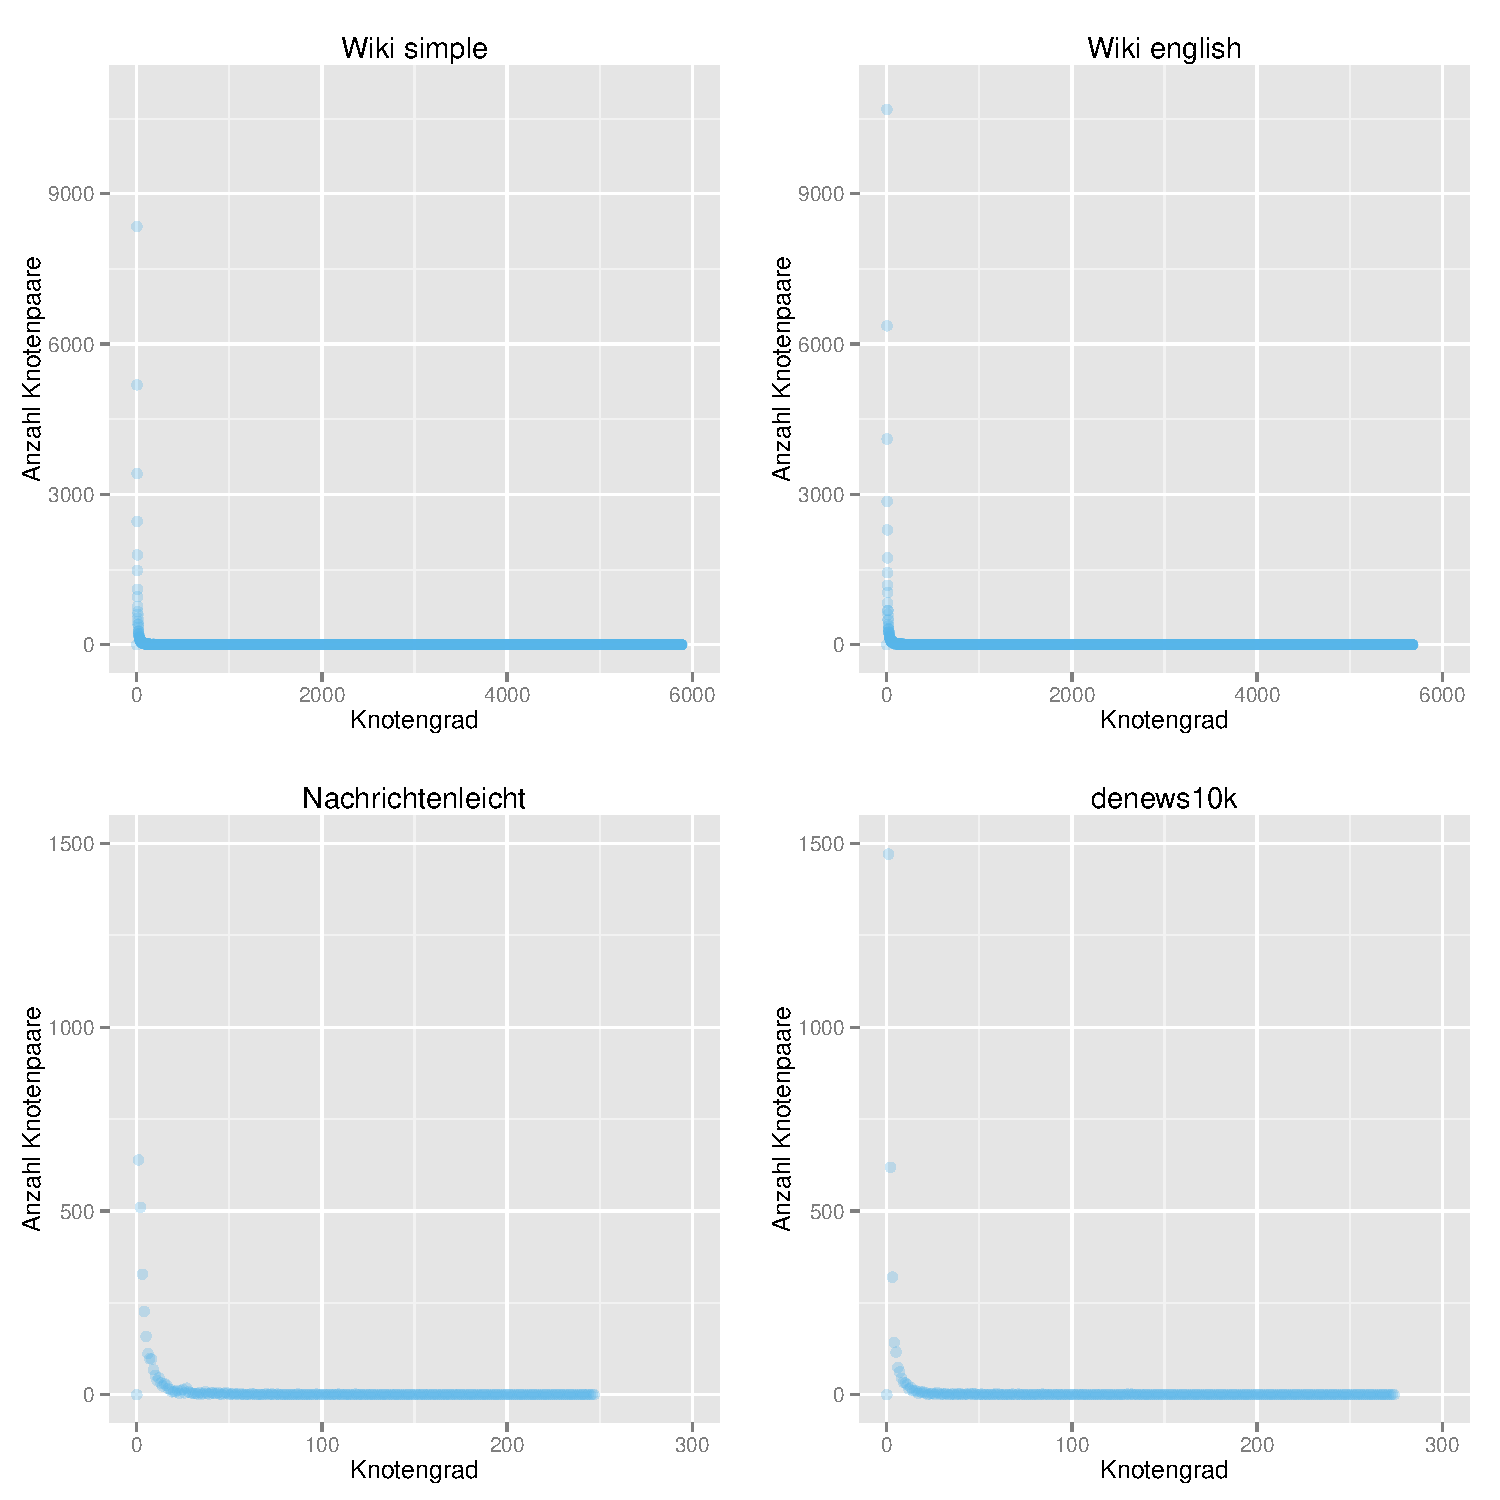
\includegraphics[scale=.5]{vdeg_plots.pdf}
        \caption{Verteilung der Knotengrade nach Corpus}
    \label{fig-vdeg}
\end{figure}

\begin{figure}[ht]
    \centering
        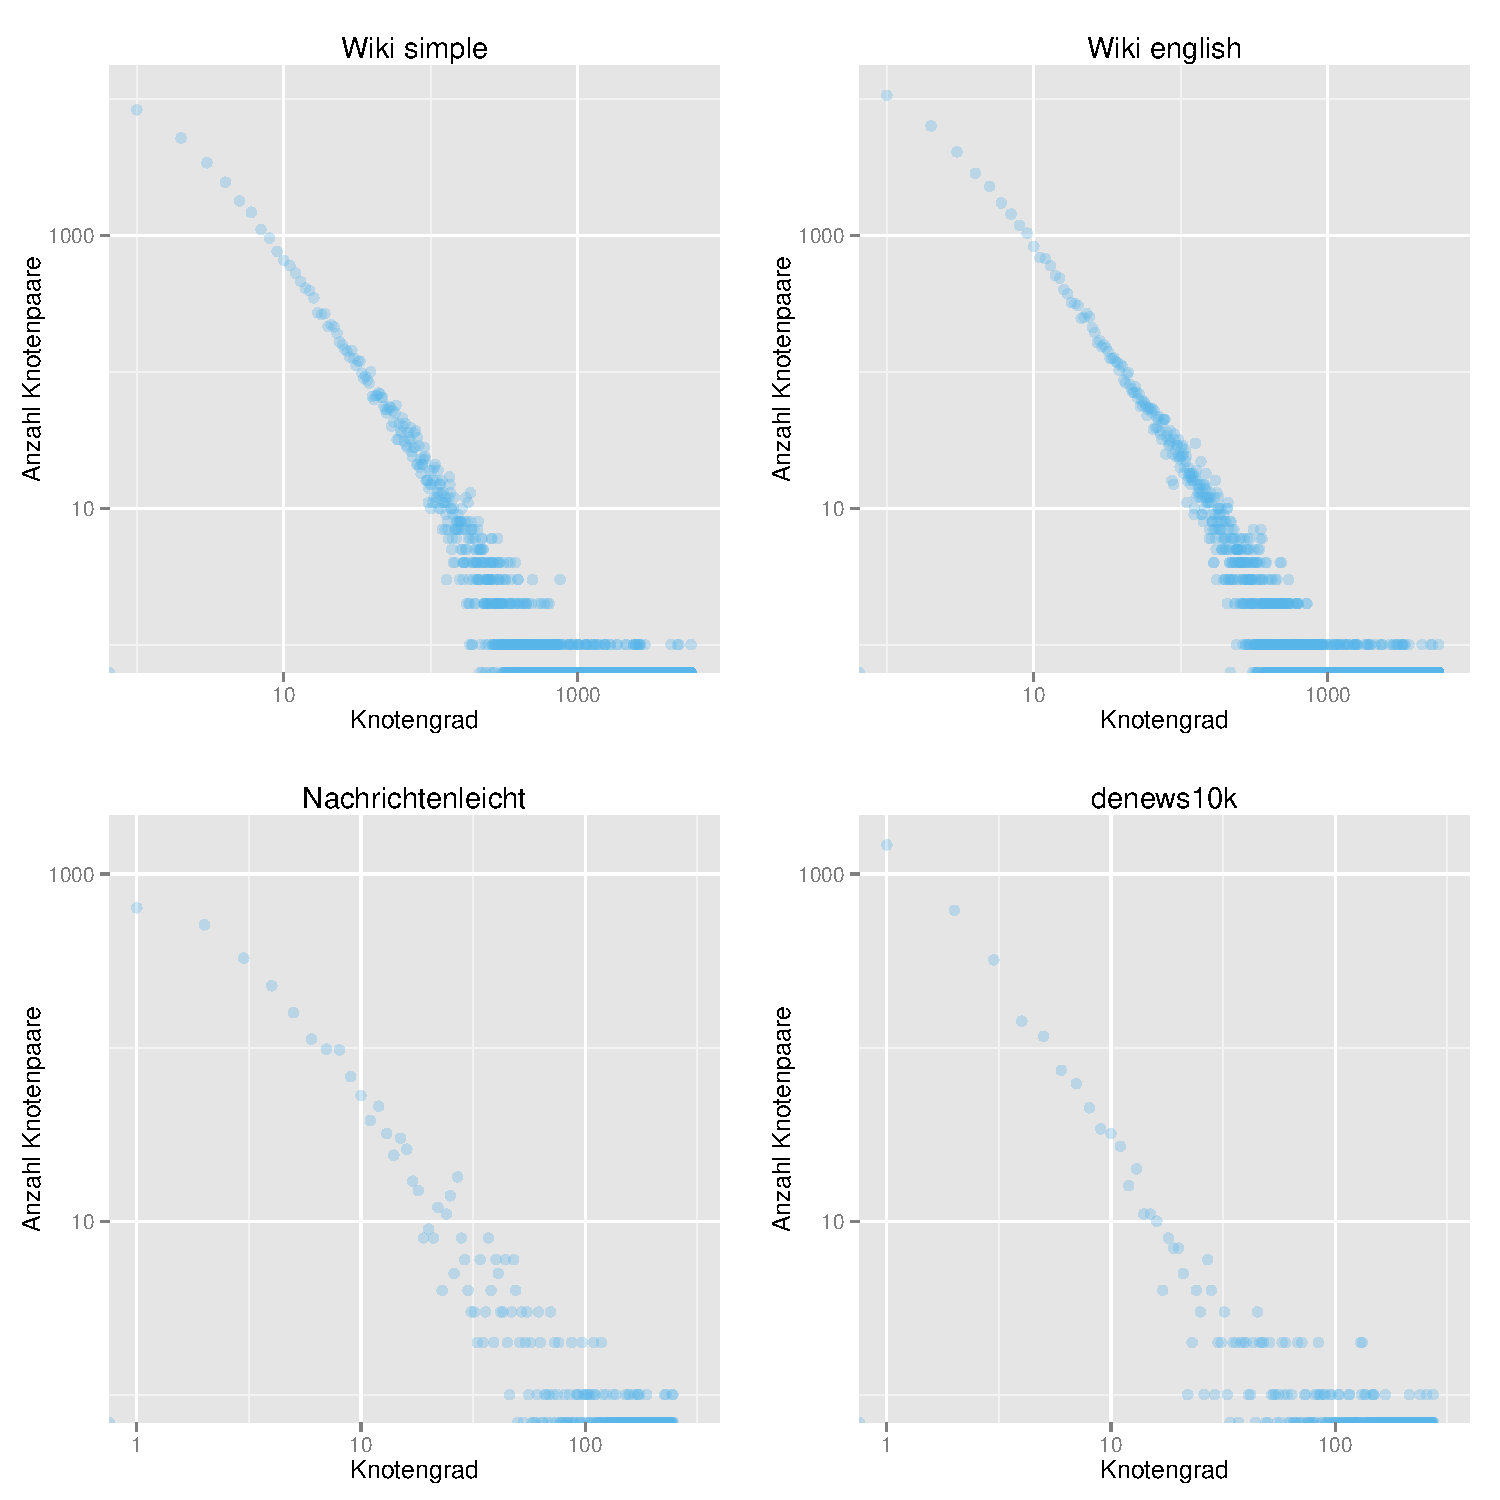
\includegraphics[scale=.5]{vdeg_plots_log.pdf}
        \caption{Verteilung der Knotengrade nach Corpus (Achsen logarithmisch skaliert)}
    \label{fig-vdeg-log}
\end{figure}


\subsection{Dichte}

Die Dichte eines Graphen beschreibt das Verhältnis von vorhandenen Kanten zu
potentiell möglichen Kanten.
Ein Wert von $1$ bedeutet, dass jeder Knoten mit jedem anderen verbunden ist
(vollständiger Graph).
Dem gegenüber bedeutet eine $0$, dass keine Kanten vorhanden sind.
Die Dichte wird wie folgt berechnet:

$$
    \frac{|E|}{|V|\left(|V|-1\right)}
$$
$|E|$ ist die Anzahl der Kanten, $|V|$ die Anzahl der Knoten im Graphen. 

Für die einfachen Sprachvarianten sollten unseren Erwartungen zufolge die
Graphen dichter sein als für Standardsprache.
Wie bereits beschrieben, gibt es in ersteren weniger Vokabular, dementsprechend
weniger Knoten, die potentiell verbunden werden können. Die Vorhandenen kommen
jedoch öfter gemeinsam vor und wären somit enger verknüpft.

\begin{table}[ht]
  \centering
  \begin{tabular}{lr}
    \toprule
    Corpus            &         Dichte (in $10^{-4}$)\\
    \midrule
    nl                &  		15,090239 \\
    denews            &  		7,737342 \\
    wiki\_sim         &  		2,844456 \\
    wiki\_en          &  		2,489951 \\
    \bottomrule
  \end{tabular}
  \caption{\label{density_table} Graphdichte nach Corpus}
\end{table}

Die Ergebnisse in Tabelle \ref{density_table} bestätigen diese Vermutung.
Insgesamt haben alle Graphen eine Dichte von $<0,01$, was für
Kookkurrenzgraphen in einem erwartbaren Rahmen liegt.

Der nachrichtenleicht-Graph weist mit $15,1\cdot 10^{-4}$ eine fast doppelt so
hohe Dichte auf wie denews ($7,74\cdot 10^{-4}$).\\
Bei den englischen Corpora fällt der Unterschied etwas geringer aus.
Dennoch weist die reguläre Sprachvariante auch hier eine ca. 14\% geringere
Dichte auf als die Leichte Sprache.

Dass die Graphen der Wikipedia-Corpora eine geringere Dichte haben, lässt sich
mit der in einer Enzyklopädie zu erwartenden höheren Themenvielfalt gegenüber
den Nachrichteninhalten erklären.
Dies bedeutet mehr potentiell auftretende unterschiedliche Wörter, die jedoch
nicht alle in den gleichen Kontexten auftreten und somit nur in begrenztem
Umfang Kanten zum Graphen hinzufügen.
Der Quadratische Zusammenhang der Dichte
führt somit zu deutlich niedrigeren Werten. 


\subsection{Small-World-Eigenschaften}

Small-World-Graphen zeichnen sich durch kleine Durchmesser und hohe Clusterkoeffizienten aus.
Diese Werte sind im Vergleich zu Zufallsgraphen zu betrachten.
Dementsprechend gibt es Messwerte, die versuchen, genau diese Relation in einem Wert zusammenzufassen, um damit eine Aussage über Small-World-Eigenschaften zu machen. 


\subsubsection{Clusterkoeffizient}

Der Clusterkoeffizient ist eng mit der Dichte verwandt. Er beschreibt die
Anzahl vorhandener Dreiecke im Graph im Verhältnis zu möglichen Dreiecken. Drei
Knoten, die jeweils paarweise verbunden sind, bilden ein Dreieck. Ziel ist ein
Messwert, der aussagt, wie sehr die Knoten Cliquen bilden. Lokal betrachtet
kennzeichnet dieser Wert die Wahrscheinlichkeit, dass ein Knoten mit den
Nachbarknoten seiner Nachbarknoten verbunden ist.

Da wir die Graphen global miteinander vergleichen möchten, verwenden wir den
globalen Clusterkoeffizienten $C$. Er berechnet sich wie folgt:

$$
    C = \frac{3\cdot\text{Anzahl der Dreiecke}}{\text{Anzahl verbundener Tripel}}
$$

Ein Tripel bezeichnet drei beliebig miteinander verbundene Knoten (nicht
notwendigerweise ein Dreieck). Knoten A kann mit Knoten B und C verbunden sein,
während B nicht mit C verbunden ist.

In \emph{Small-World-Graphen} ist der Clusterkoeffizient typischerweise hoch, 
insbesondere verglichen mit Zufallsgraphen gleicher Größe, also gleicher Anzahl
Knoten und Kanten \cite{Newman2003}.


\subsubsection{Durchmesser und minimale Wegl\"angen}

Auch die Betrachtung von Weglängen erlaubt Rückschlüsse auf die Small-World-Eigenschaften.
Eine gute Kenngröße ist dabei der Durchmesser
des Graphen, also der längste minimale Weg zwischen zwei Knoten. In einer
\emph{small world} sind alle Knoten von allen anderen in wenigen Schritten
erreichbar\footnote{typischerweise sind dies bei realen Netzwerken etwa 6 Schritte, die sogenannten 
\emph{six degrees of separation}\cite{Newman2003}}.

\texttt{graph-tool} erlaubt zum einen die Ausgabe eines Durchmessers, wie oben
beschrieben, und zum anderen die Ausgabe eines Histogramms, welches die 
Häufigkeit der Längen aller kürzesten Wege darstellt (siehe Abb. \ref{fig-mdh}).

% latex table generated in R 3.2.0 by xtable 1.7-4 package
% Mon Apr 20 13:50:42 2015
\begin{table}[ht]
    \centering
    \begin{tabular}{*{5}{r}}
      \toprule
    Weglänge       & nl          & denews      & wiki\_sim   & wiki\_en     \\ 
      \midrule
      1            & 0,30        & 0,15        & 0,06        & 0,05         \\ 
      2            & 10,66       & 6,69        & 14,94       & 12,95        \\ 
      3            & 49,35       & 46,26       & 63,60       & 64,48        \\ 
      4            & 34,55       & 41,83       & 20,25       & 21,30        \\ 
      5            & 4,61        & 4,70        & 1,11        & 1,17         \\ 
      6            & 0,47        & 0,35        & 0,04        & 0,04         \\ 
      7            & 0,07        & 0,01        & $\sim$0,00  & $\sim$0,00   \\ 
      8            & $\sim$0,00  & $\sim$0,00  & $\sim$0,00  & $\sim$0,00   \\ 
      9            & $\sim$0,00  & 0           & 0           & 0            \\ 
      Summe        & 100,00      & 100,00      & 100,00      & 100,00       \\ 
      Durchschnitt & 3,34        & 3,45        & 3,08        & 3,11         \\
       \bottomrule
    \end{tabular}
    \caption{Anteil der Weglängen paarweiser kürzester Wege zwischen allen Knoten, in Prozent}
    \label{md-perc}
\end{table}

\begin{figure}[ht]
    \centering
        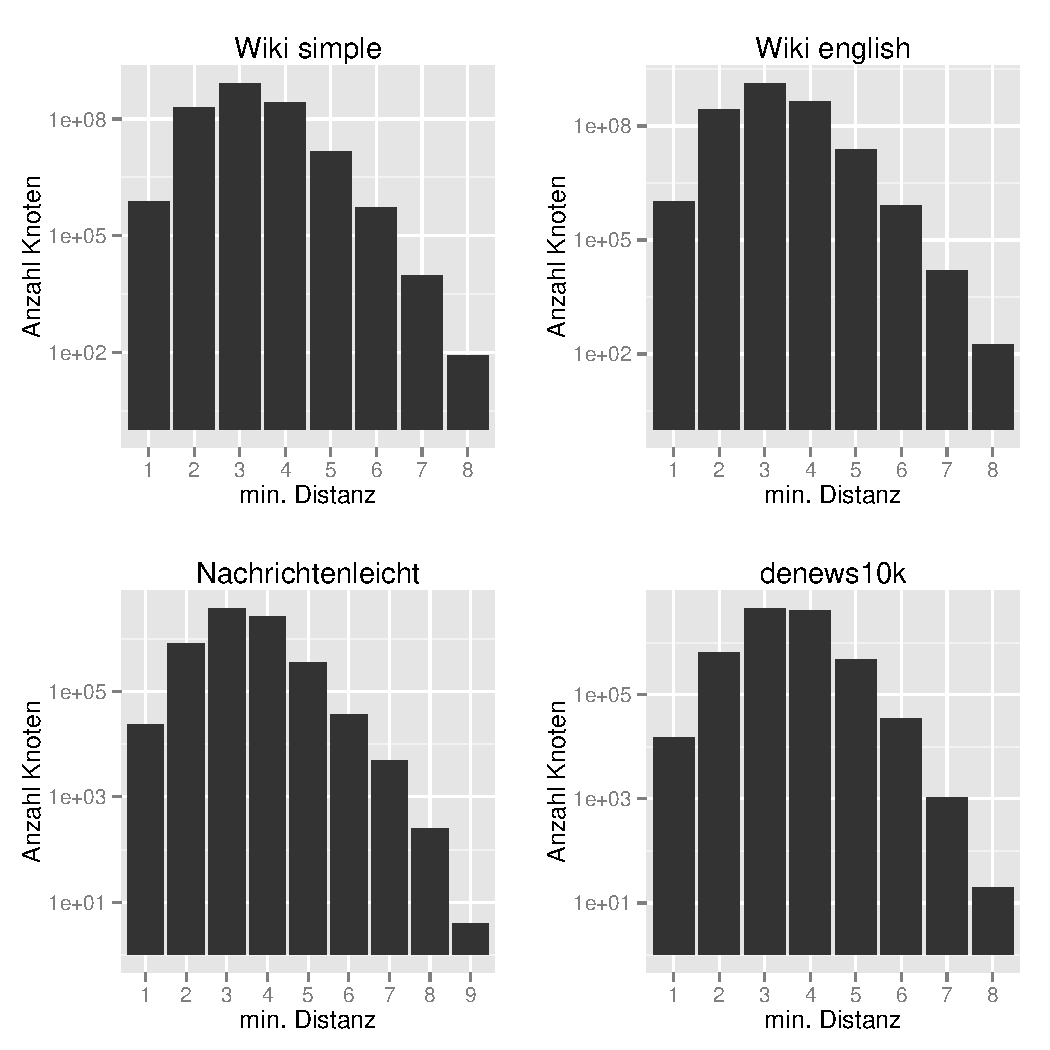
\includegraphics[scale=.75]{mdh_plots.pdf}
    \caption{Verteilung der minimalen Weglängen nach Corpus}
    \label{fig-mdh}
\end{figure}


\subsubsection{Small-World-Messwert}

Humphries et al. führen in \cite{Humphries2006} einen Messwert ein, der deutlich
machen soll, ob ein Graph ein Small-World-Graph ist oder nicht. Sie setzen hierzu
die Weglängen und die globalen Clusterkoeffizienten von Graphen zueinander in 
Relation.

Dabei sollen sich Small-World-Graphen insbesondere durch einen hohen
 Clusterkoeffizienten auszeichnen, wogegen kurze Weglängen besonders
 Zufallsgraphen charakterisieren. Um diese Erkentnisse zu verbinden, werden die
 beiden Messwerte des zu testenden Graphen mit denen eines vergleichbaren
 Zufallsgraphen relativiert. Der Zufallsgraph wird aus dem Ursprünglichen durch
 zufallsbasiertes \emph{rewiring} gewonnen.
Dabei werden alle Kanten jeweils neu verbunden, unter Beibehaltung der Verteilung
der Knotengrade.
Jede neu zu erstellende Verbindung hat dabei die gleiche Wahrscheinlichkeit.

Auch dieses Verfahren wird von \texttt{graph\_tool} unterstützt\footnote{vgl. Algorithmus unter \url{http://graph-tool.skewed.de/static/doc/generation.html\#graph_tool.generation.random_rewire}}.

Das Small-World-Maß setzt sich wie folgt zusammen:

$$
\sigma = \frac{C/C_{rand}}{ L/L_{rand}}
$$

Dabei ist $L$ der durchschnittliche kürzeste Abstand zwischen den Knoten und $C$
der Clusterkoeffizient.
Wichtigstes Kennzeichen für einen Small-World-Graphen ist,
dass $C \gg C_{rand}$, während $L \approx L_{rand}$, so dass $\sigma > 1$.\cite{Humphries2006}

\subsubsection{Ergebnisse}
Tabelle \ref{tab-zsf} enthält die Ergebnisse der Berechnungen.

\paragraph{Clusterkoeffizient}
Zwischen den beiden deutschen Corpora bestehen große Unterschiede.
In Leichter Sprache ergibt sich ein Wert von etwa $0,06$, wogegen dieser bei normaler Sprache lediglich $0,03$ beträgt.
Die Leichte Sprache ist hier also deutlich stärker geclustert.

Die Wikipedia-Graphen weisen zueinander ähnliche Werte auf, die beide knapp über 0,04 liegen.

Verglichen mit Graphen aus \cite[S. 182]{Newman2003} sind die Werte jedoch alle sehr klein.
Insbesondere der Vergleich zu Zufallsgraphen gleicher Größe ist interessant:
Der Quotient aus $C/C_{rand}$ ist in allen Fällen unter $1$, für den nachrichtenleicht-Graphen liegt er bei $0,96$.
Der ursprüngliche Graph und sein zufällig verändertes Pendant haben also beinahe denselben Clusterkoeffizienten.

Zusammengefasst ist deutlich erkennbar, dass die Clusterkoeffizienten nicht in Wertebereichen liegen, die für Small-World-Eigenschaften notwendig wären.

\paragraph{Durchmesser und Weglängen}
Für die Graphdurchmesser zeigen sich jedoch andere Ergebnisse.
Typischerweise lassen sich alle Knoten innerhalb von etwa 6 Schritten von jedem anderen Knoten aus erreichen.
Tabelle \ref{md-perc} bestätigt diese These.
Es befinden sich nur wenige Wortpaare außerhalb dieser Grenze.
Diese werden im nächsten Abschnitt und Kapitel \ref{sec:aussen_liegende} mit Hilfe von Visualisierungen detailierter betrachtet.

Es zeigt sich bei allen untersuchten Graphen, dass deren Ränder aus selten verwendeten Namen bestehen.
Die Tabelle zeigt sehr deutlich, dass die meisten Paare innerhalb von 3-4 Schritten verbunden sind.
Längere Pfade treten nur selten auf.
Die durchschnittlichen Weglängen liegen bei allen vier Graphen knapp über 3.
Für Small-World-Graphen wäre lt. Newmann ein etwas höherer Durchschnitt typischer gewesen (vgl. \cite{Newman2003}).
Bei sozialen Netzwerken bewegen sich die Weglängen nach seinen Angaben typischerweise um $5$-$7$.
Für den dort ebenfalls erwähnten Wortkookkurrenzgraphen ist leider kein Wert angegeben.

\paragraph{Außen liegende Wörter}
Wie oben beschrieben, machen überwiegend Namen den äußeren Rand der Graphen aus.
So sind etwa \emph{Seymour} und \emph{Hoffman} (Abb. \ref{fig:lp-hoffman}) im nachrichtenleicht-Graphen lediglich ein mal vorgekommen, im Zuge der Todesnachricht des Schauspielers.

Im englischsprachigen wiki\_sim-Graphen liegen \emph{(Che) Guevara}, \emph{Kamui (Kobayashi)}, \emph{Kazimir Malevich} und die \emph{Frankfurter Allgemeine Zeitung} ganz außen.
Auch hier ist also zu beobachten, dass Eigennamen -- insbesondere fremdsprachige -- die Graphgrenzen ausmachen.

Beim denews-Graphen sind \emph{Microsoft}, \emph{Windows}, und \emph{Phone} in Zusammenhang außen, oder auch \emph{Financial} und \emph{Times}, jedoch auch \emph{Metzelder} und \emph{(St.) Pauli} (Abb. \ref{fig:lp-pauli}).

Bei Größen von 10.000 Sätzen ist es bei den Nachrichtencorpora nicht verwunderlich, dass aufgrund der Unterschiedlichkeit von behandelten Themen selten genannte Personen am Rand des Graphen erscheinen.
Da die Nachrichten in sehr begrenzten Zeiträumen gesammelt wurden, verstärkt sich dieser Effekt.

Ein ähnliches Phänomen ist bei den Wikipediaartikeln zu beobachten, welche thematisch unabhängig voneinander sind.
Hier sind stark vernetzte Cluster aus verschiedenen Themengebieten zu erwarten, die wenig mit anderen, thematisch anders gelagerten, Clustern verbunden sind.

Namen von Personen, die stärker im Fokus der Öffentlichkeit stehen, etwa \emph{Angela}, \emph{Merkel} und \emph{Obama}, sind verglichen zu den oben genannten deutlich stärker im Graph verbunden.
Auch die dort verbundenen Wörter sind ein Hinweis darauf, ob ein Wort am Rand oder im Graphen liegt.
Verben wie \emph{sagt} verbinden sehr schnell zum Zentrum.

\paragraph{Small-World-Messwert}
Wie die Ergebnisse der Clusterkoeffizienten bereits andeuten, lässt sich mit dem verwendeten Maß nicht nachweisen, dass es sich bei den Kookkurrenzgraphen um Small-World-Graphen handelt.
Die Zwischenrechnungen und Ergebnisse sind in \ref{tab-zsf} zu sehen.
Zwar sind die durchschnittlichen Weglängen bei den Zufallsgraphen beinahe identisch zu denen der Ursprungsgraphen, jedoch bilden die Wortcorpora nicht genügend Cluster, um die Anforderungen an Small-World-Graphen zu erfüllen.
$C/C_{rand}$ liegt teilweise derart nah beieinander, dass den Graphen lediglich Ähnlichkeit zu Zufallsgraphen nachweisbar ist.
Bei denews liegt er -- bedingt durch die geringe Dichte -- sogar unter $0,5$.

\begin{table}[ht]
    \begin{tabular}{l*{4}{r}}
    \toprule
    Kenngröße                     & nl        & denews    & wiki\_sim & wiki\_en \\
    \midrule
    $|V|$                          & 2946      & 3205      & 36582     & 45897  \\
    $|E|$                          & 11639     & 7669      & 371559    & 514489 \\
    $|V|$\footnotemark[6]          & 2766      & 3142      & 36131     & 45446  \\
    $|E|$\footnotemark[6]          & 11541     & 7636      & 371319    & 514248 \\
    Dichte (in $10^{-4}$)           & 15,090239 & 7,737342  & 2,844456  & 2,489951 \\
    Clusterkoeffizient             & 0,064516  & 0,033906  & 0,040403  & 0,042299 \\
    Clusterkoeff. stdev ($10^{-2}$) & 0,626338  & 0,470389  & 0,612476  & 0,481688 \\
    $\sigma$                       & 0,970016  & 0,451959  & 0,857932  & 0,897925  \\
    $C / C_{rand}$                  & 0,961374  & 0,474512  & 0,832651  & 0,869740 \\
    $L / L_{rand}$                  & 0,991090  & 1,049900  & 0,970532  & 0,968610 \\
%    \dots                         &           &           &           &          \\
    \bottomrule
    \end{tabular}
    \caption{Übersichtstabelle Graphenkenngrößen}
    \label{tab-zsf}
\end{table}
% TODO: nach dem Endlayout sicherstellen, dass die folgene Fußnote an der richtigen
% Stelle auftaucht!
\footnotetext[6]{größte Zusammenhangskomponente}


\subsection{H\"aufige W\"orter}

\subsubsection{Nachrichten-Corpora}

\begin{table}[ht]
    \begin{tabular}{l*{2}{lr}}
    \toprule
    Nr. & nl & Häufigkeit & denews & Häufigkeit\\
    \midrule
    1  & Menschen    & 87 &  Prozent     & 48 \\
    2  & gewonnen    & 69 &  Euro        & 47 \\
    3  & Mannschaft  & 62 &  sagte       & 24 \\
    4  & Geld        & 54 &  Uhr         & 23 \\
    5  & Stadt       & 51 &  Jahren      & 23 \\
    6  & mehr        & 50 &  sei         & 18 \\
    7  & Partei      & 45 &  wurde       & 18 \\
    8  & Land        & 45 &  einfach     & 17 \\
    9  & Dortmund    & 45 &  Artikel     & 16 \\
    10 & Politiker   & 43 &  \textbf{Jahr}        & 16 \\
    11 & Spiel       & 41 &  Dollar      & 15 \\
    12 & bekommen    & 41 &  verwenden   & 15 \\
    13 & \textbf{Jahr}        & 40 &  unten       & 15 \\
    14 & viele       & 38 &  Jahre       & 15 \\
    15 & Bayern      & 36 &  stehenden   & 15 \\
    16 & Preis       & 34 &  Link        & 14 \\
    17 & München     & 34 &  möchten     & 14 \\
    18 & Verein      & 33 &  verlinken   & 14 \\
    19 & deutsche    & 33 &  kostenfrei  & 14 \\
    20 & Film        & 32 &  seit        & 14 \\
    21 & zusammen    & 32 &  dpa         & 14 \\
    22 &             &    &  Millionen   & 14 \\
    \bottomrule
    \end{tabular}
    \caption{Häufigste Worte in den Nachrichten-Corpora}
    \label{words-nachrichten}
\end{table}

Wie in Tabelle \ref{words-nachrichten} zu erkennen, gibt es nur wenige
Überschneidungen des Vokabulars des nachrichtenleicht-Corpus mit denews.
Fett gedruckt sind in den Tabellen diejenigen Worte, die in beiden Corpora
vorkommen.
Bei den Nachrichten-Corpora handelt es sich lediglich um das Wort "`Jahr"'.
Dies deutet bereits auf eine gewisse thematische Inhomogenität der Corpora hin.
Dieses Ergebnis ist insofern nicht überraschend, dass die Corpora aus
unterschiedlichen Quellen stammen (vgl. Abschnitt \ref{nrseiten}) und
im Gegensatz zu den Wikipedia-Daten kein Dokumenten-Alignment vorliegt.
Auch wurden die Ursprungstexte für jeweils unterschiedliche Zielgruppen verfasst.

Darüber hinaus zeigt sich, dass Worte im nachrichtenleicht-Corpus generell
häufiger auftreten (häufigstes Wort: Menschen, 87mal; denews: Prozent, 48mal).
Dies bestätigt die Vermutung aus Abschnitt \ref{groesse-knotenzahl} bzgl. der
Knotenanzahl.

Weiterhin wird ersichtlich, dass der nachrichtenleicht-Corpus seinen
thematischen Schwerpunkt auf Politik und Sport legt.
Erkennbar ist dies am häufigen Auftreten der Worte wie \emph{Stadt}, \emph{Partei}, \emph{Land},
\emph{Politiker} bzw. \emph{Mannschaft}, \emph{Spiel}, \emph{Bayern}, \emph{München}, \emph{Verein}.
Im denews-Corpus treten hingegen häufiger wirtschaftsbezogene Wörter wie \emph{Prozent},
\emph{Euro}, \emph{Dollar} oder \emph{Millionen} auf.


\subsubsection{Wikipedia-Corpora}

\begin{table}[ht]
    \begin{tabular}{l*{2}{lr}}
    \toprule
    Nr. & wiki\_sim & Häufigkeit & wiki\_en & Häufikeit\\
    \midrule
     1 & \textbf{born}       & 71 & \textbf{born}         & 86\\
     2 & \textbf{American}   & 52 & \textbf{American}     & 58\\
     3 & \textbf{commune}    & 49 & \textbf{commune}      & 52\\
     4 & \textbf{France}     & 47 & \textbf{France}       & 50\\
     5 & \textbf{won}        & 41 & \textbf{department}   & 49\\
     6 & \textbf{department} & 41 & film                  & 46\\
     7 & movie               & 36 & \textbf{television}   & 43\\
     8 & \textbf{television} & 35 & \textbf{won}          & 42\\
     9 & died                & 33 & \textbf{League}       & 40\\
    10 & people              & 33 & \textbf{County}       & 40\\
    11 & NHL                 & 31 & \textbf{Award}        & 39\\
    12 & actor               & 31 & University            & 39\\
    13 & \textbf{World}      & 30 & series                & 38\\
    14 & United              & 29 & \textbf{released}     & 38\\
    15 & \textbf{League}     & 28 & album                 & 38\\
    16 & National            & 28 & professional          & 35\\
    17 & \textbf{years}      & 28 & located               & 34\\
    18 & \textbf{released}   & 28 & season                & 33\\
    19 & \textbf{Award}      & 27 & \textbf{World}        & 33\\
    20 & \textbf{County}     & 27 & \textbf{years}        & 31\\
    21 & played              & 27 & city                  & 31\\
    22 & year                & 27 &                       & \\
    \bottomrule
    \end{tabular}
    \caption{Häufigste Worte in den Wiki-Corpora}
    \label{words-wiki}
\end{table}

Bei den Wikipedia-Corpora zeigen die Ergebnisse eine hohe Übereinstimmung des
Vokabulars zwischen beiden Sprachvarianten, was für eine größere thematische
und strukturelle Homogenität als bei den Nachrichtencorpora spricht.
Die häufigsten vier Worte sind bei beiden Corpora identisch.
Insgesamt stimmen über $50\%$ der Worte überein - lediglich die Rangfolge
variiert leicht.
Dies ist angesichts des Dokumentenalignments zwischen beiden Corpora (vgl.
Abschnitt \ref{corp-wiki}) zu erwarten gewesen.

Interessant ist, dass die Simple-English-Variante etwa das Wort \emph{movie}
favorisiert, während in der Standardsprache das Synonym \emph{film} verwendet
wird.

Anders als bei den Nachrichten-Corpora sind hier bei der Leichte-Sprache-Variante
geringere Worthäufigkeiten als bei der Standardsprache zu beobachten.
Die Größenordnung dieses Unterschieds ist allerdings nicht so gravierend wie bei
den ersteren.\\
Eine mögliche Erklärung ist, dass wir beim Erstellen des Corpus die
Artikel nach Satzanzahl, nicht nach Wortanzahl normalisiert haben (wie in
Abschnitt \ref{datextr} beschrieben).
Da die Standard-English-Wikipedia längere Sätze verwendet als die Einfache,
sind in logischer Folge auch größere Worthäufigkeiten zu erwarten, denn längere
Sätze bedeuten mehr Wörter.


\clearpage
\section{Kookkurrenzgraphen}
\label{sec:graphen}

\subsection{Häufige Wörter}

Zur Erzeugung der folgenden Kookkurrenzgraphen der häufigsten Wörter
wurde der Kookkurrenz-Schwellwert individuell auf den jeweiligen Corpus
angepasst, damit unwichtige Kanten und Knoten die Graphen nicht überladen.
Es zeigte sich, dass je nach Corpus unterschiedliche Schwellwerte gewählt werden
mussten, um gut lesbare, nicht überfrachtete Graphen mit einer übersichtlichen
Anzahl an Knoten zu erzeugen.

In diesen Graphen sind jeweils nur die direkten Nachbarknoten des gesuchten
Wortes dargestellt, d.h. die Knotendistanz beträgt immer 1.

\subsubsection{nachrichtenleicht.de}

\begin{figure}[hp!]
    \centering
        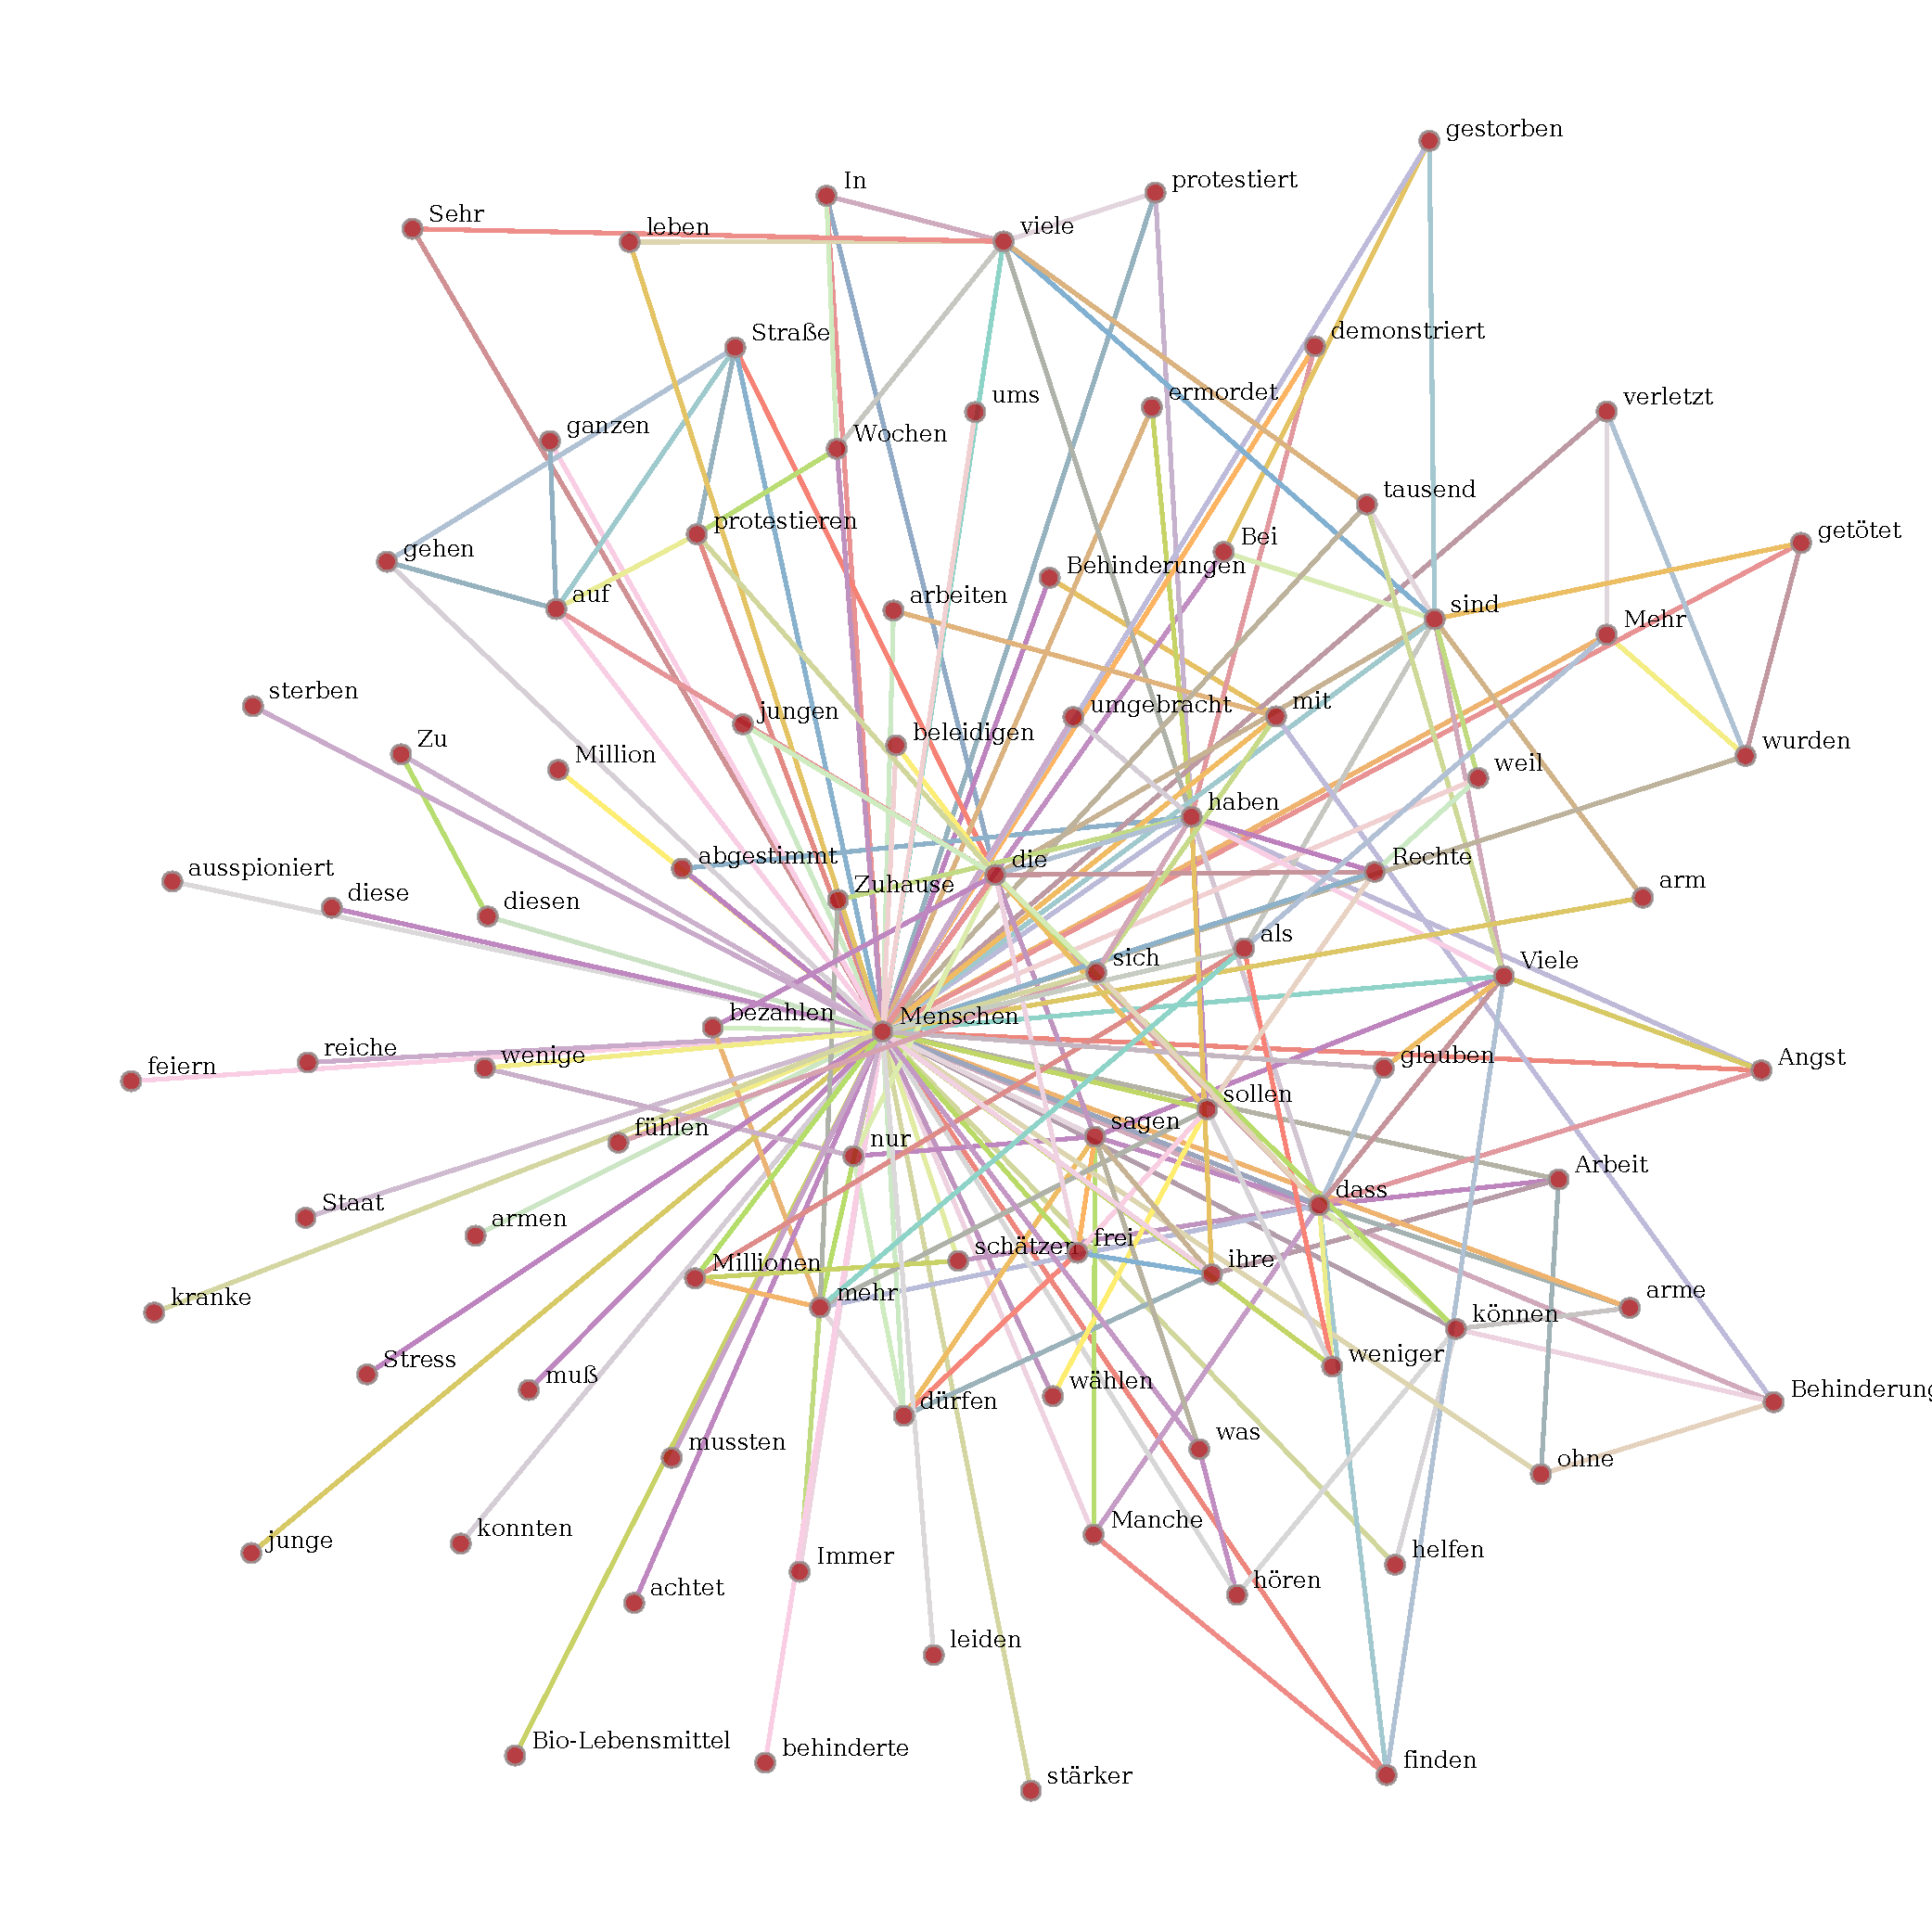
\includegraphics[scale=.4]{../../data/results/cooc_nl/topwords/graph_Menschen.pdf}
    \caption{Kookkurrenzgraph Menschen (Distanz 1, Schwellwert 1/12, Häufigkeit 87)}
    \label{fig:hw-menschen}
\end{figure}

\begin{figure}[hp!]
    \centering
        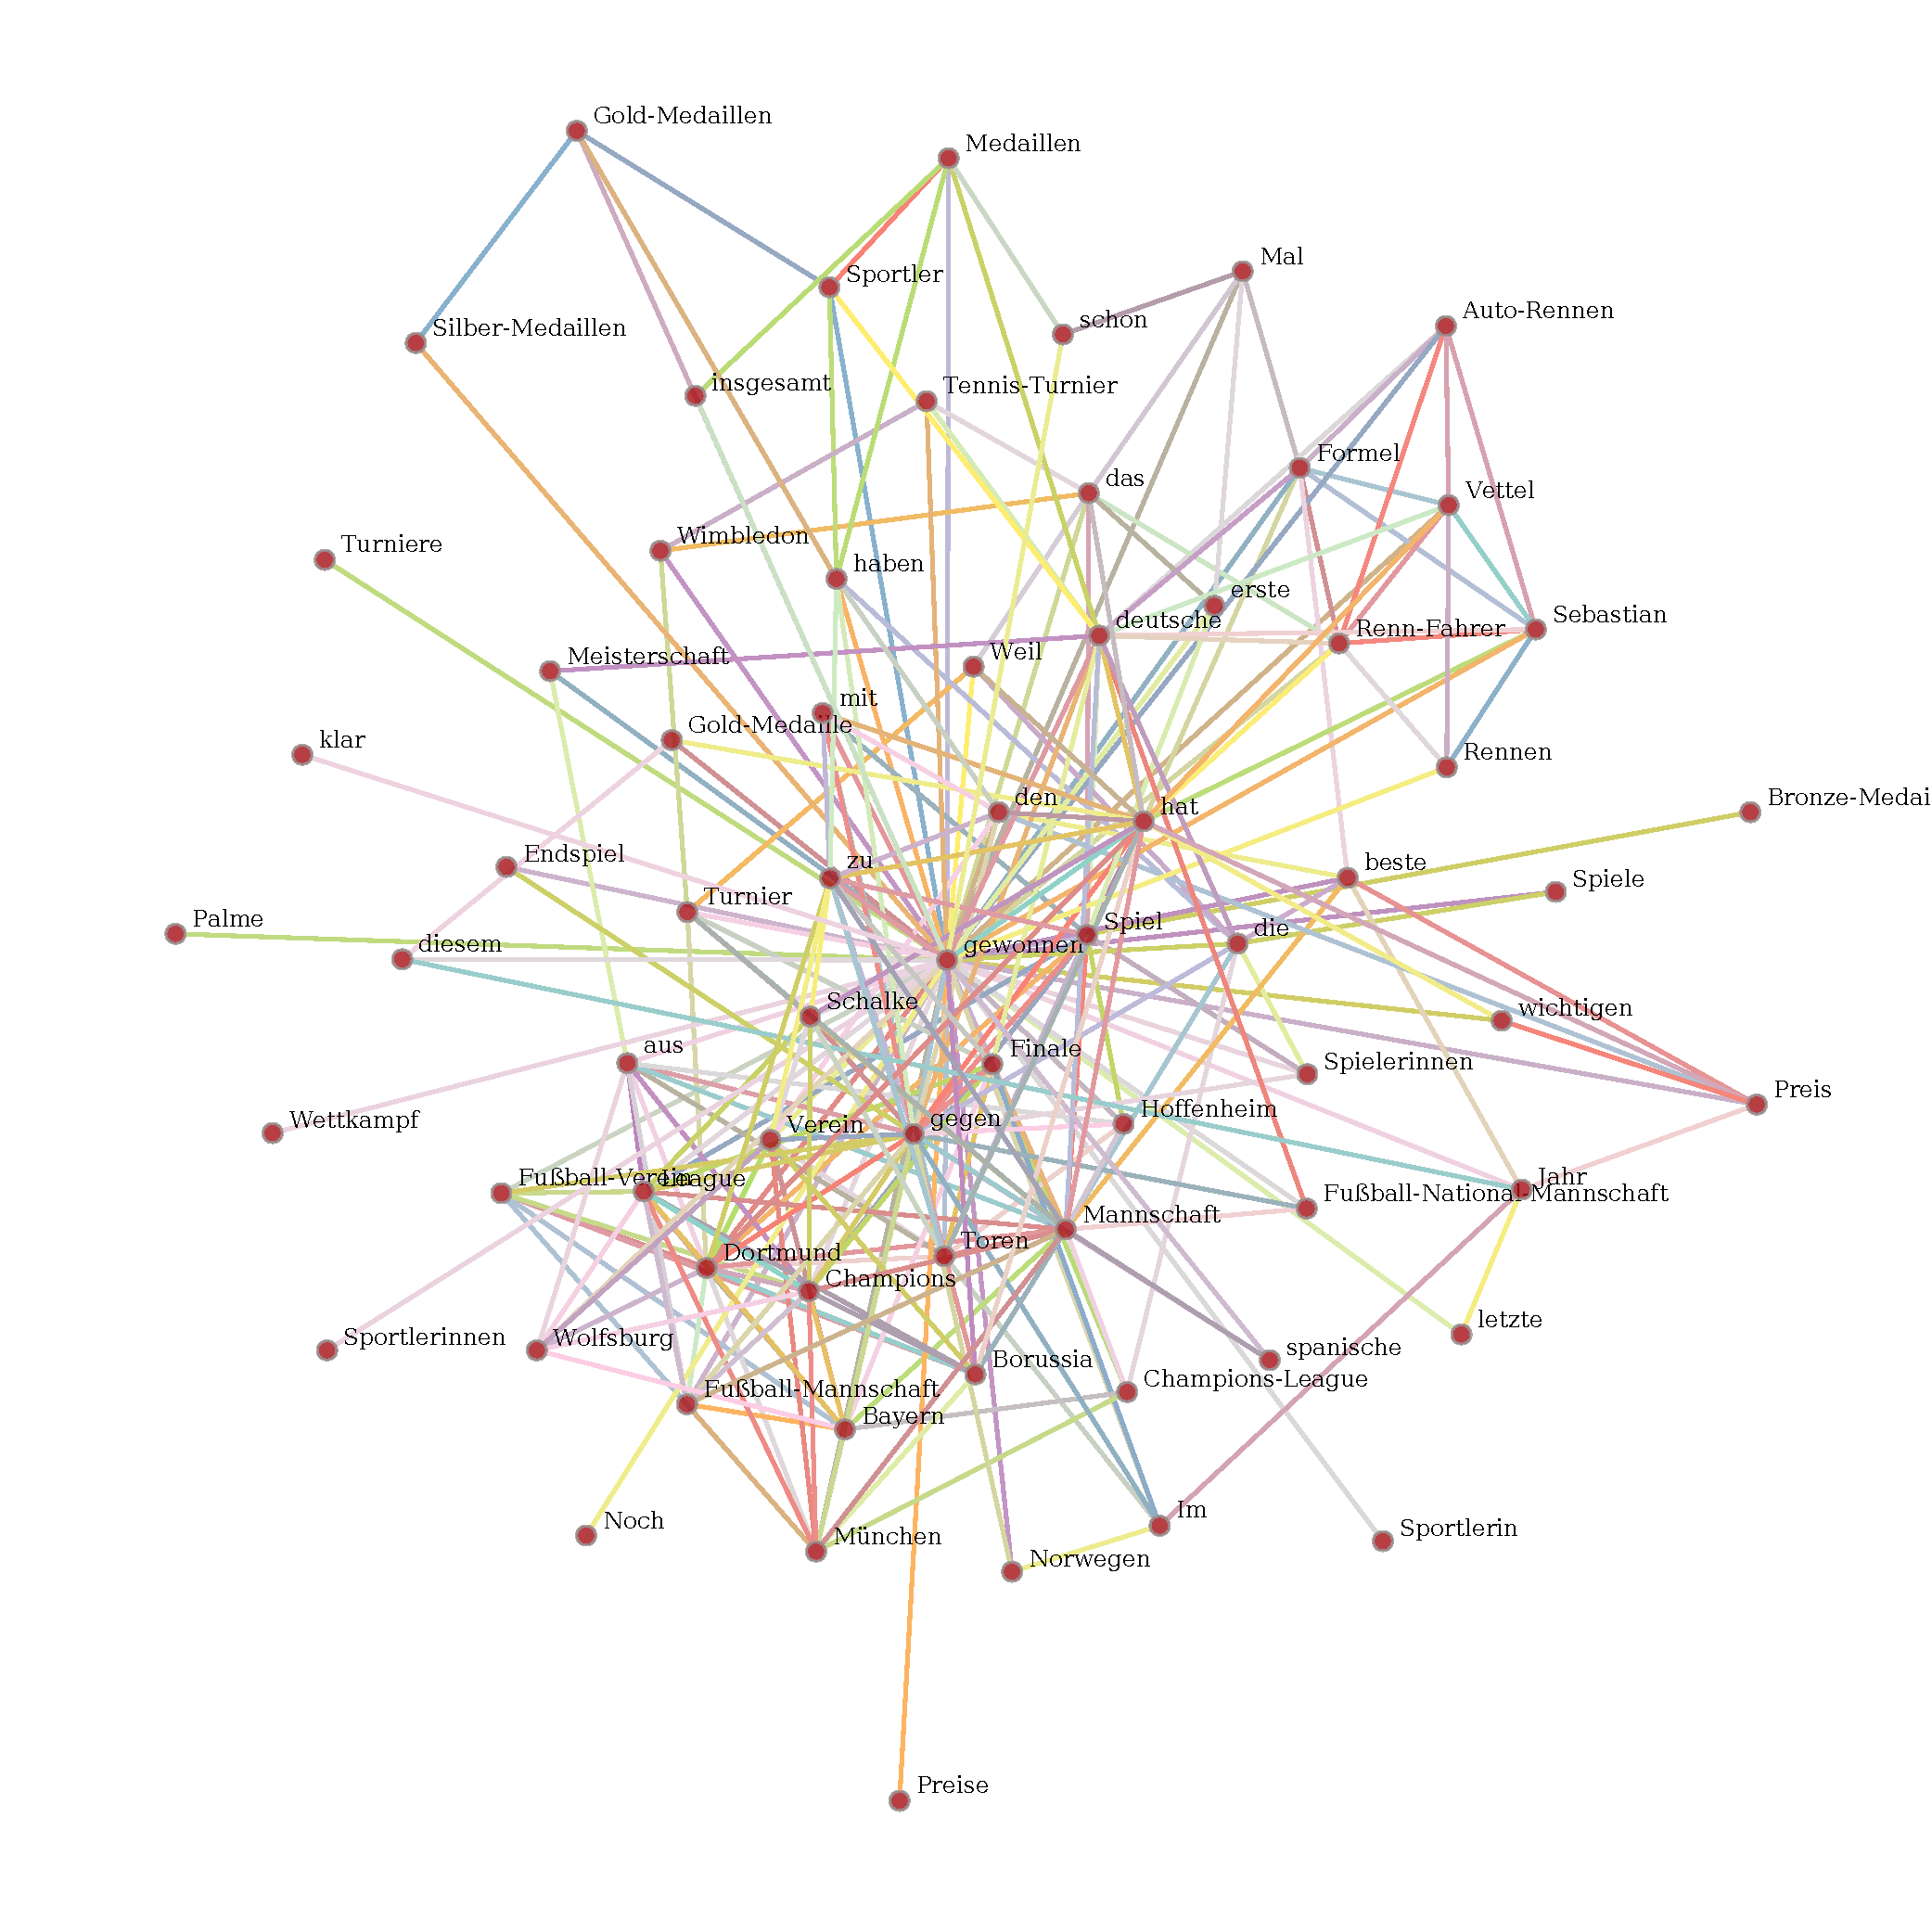
\includegraphics[scale=.4]{../../data/results/cooc_nl/topwords/graph_gewonnen.pdf}
    \caption{Kookkurrenzgraph gewonnen (Distanz 1, Schwellwert 1/12, Häufigkeit 69)}
    \label{fig:hw-gewonnen}
\end{figure}

\begin{figure}[hp!]
    \centering
        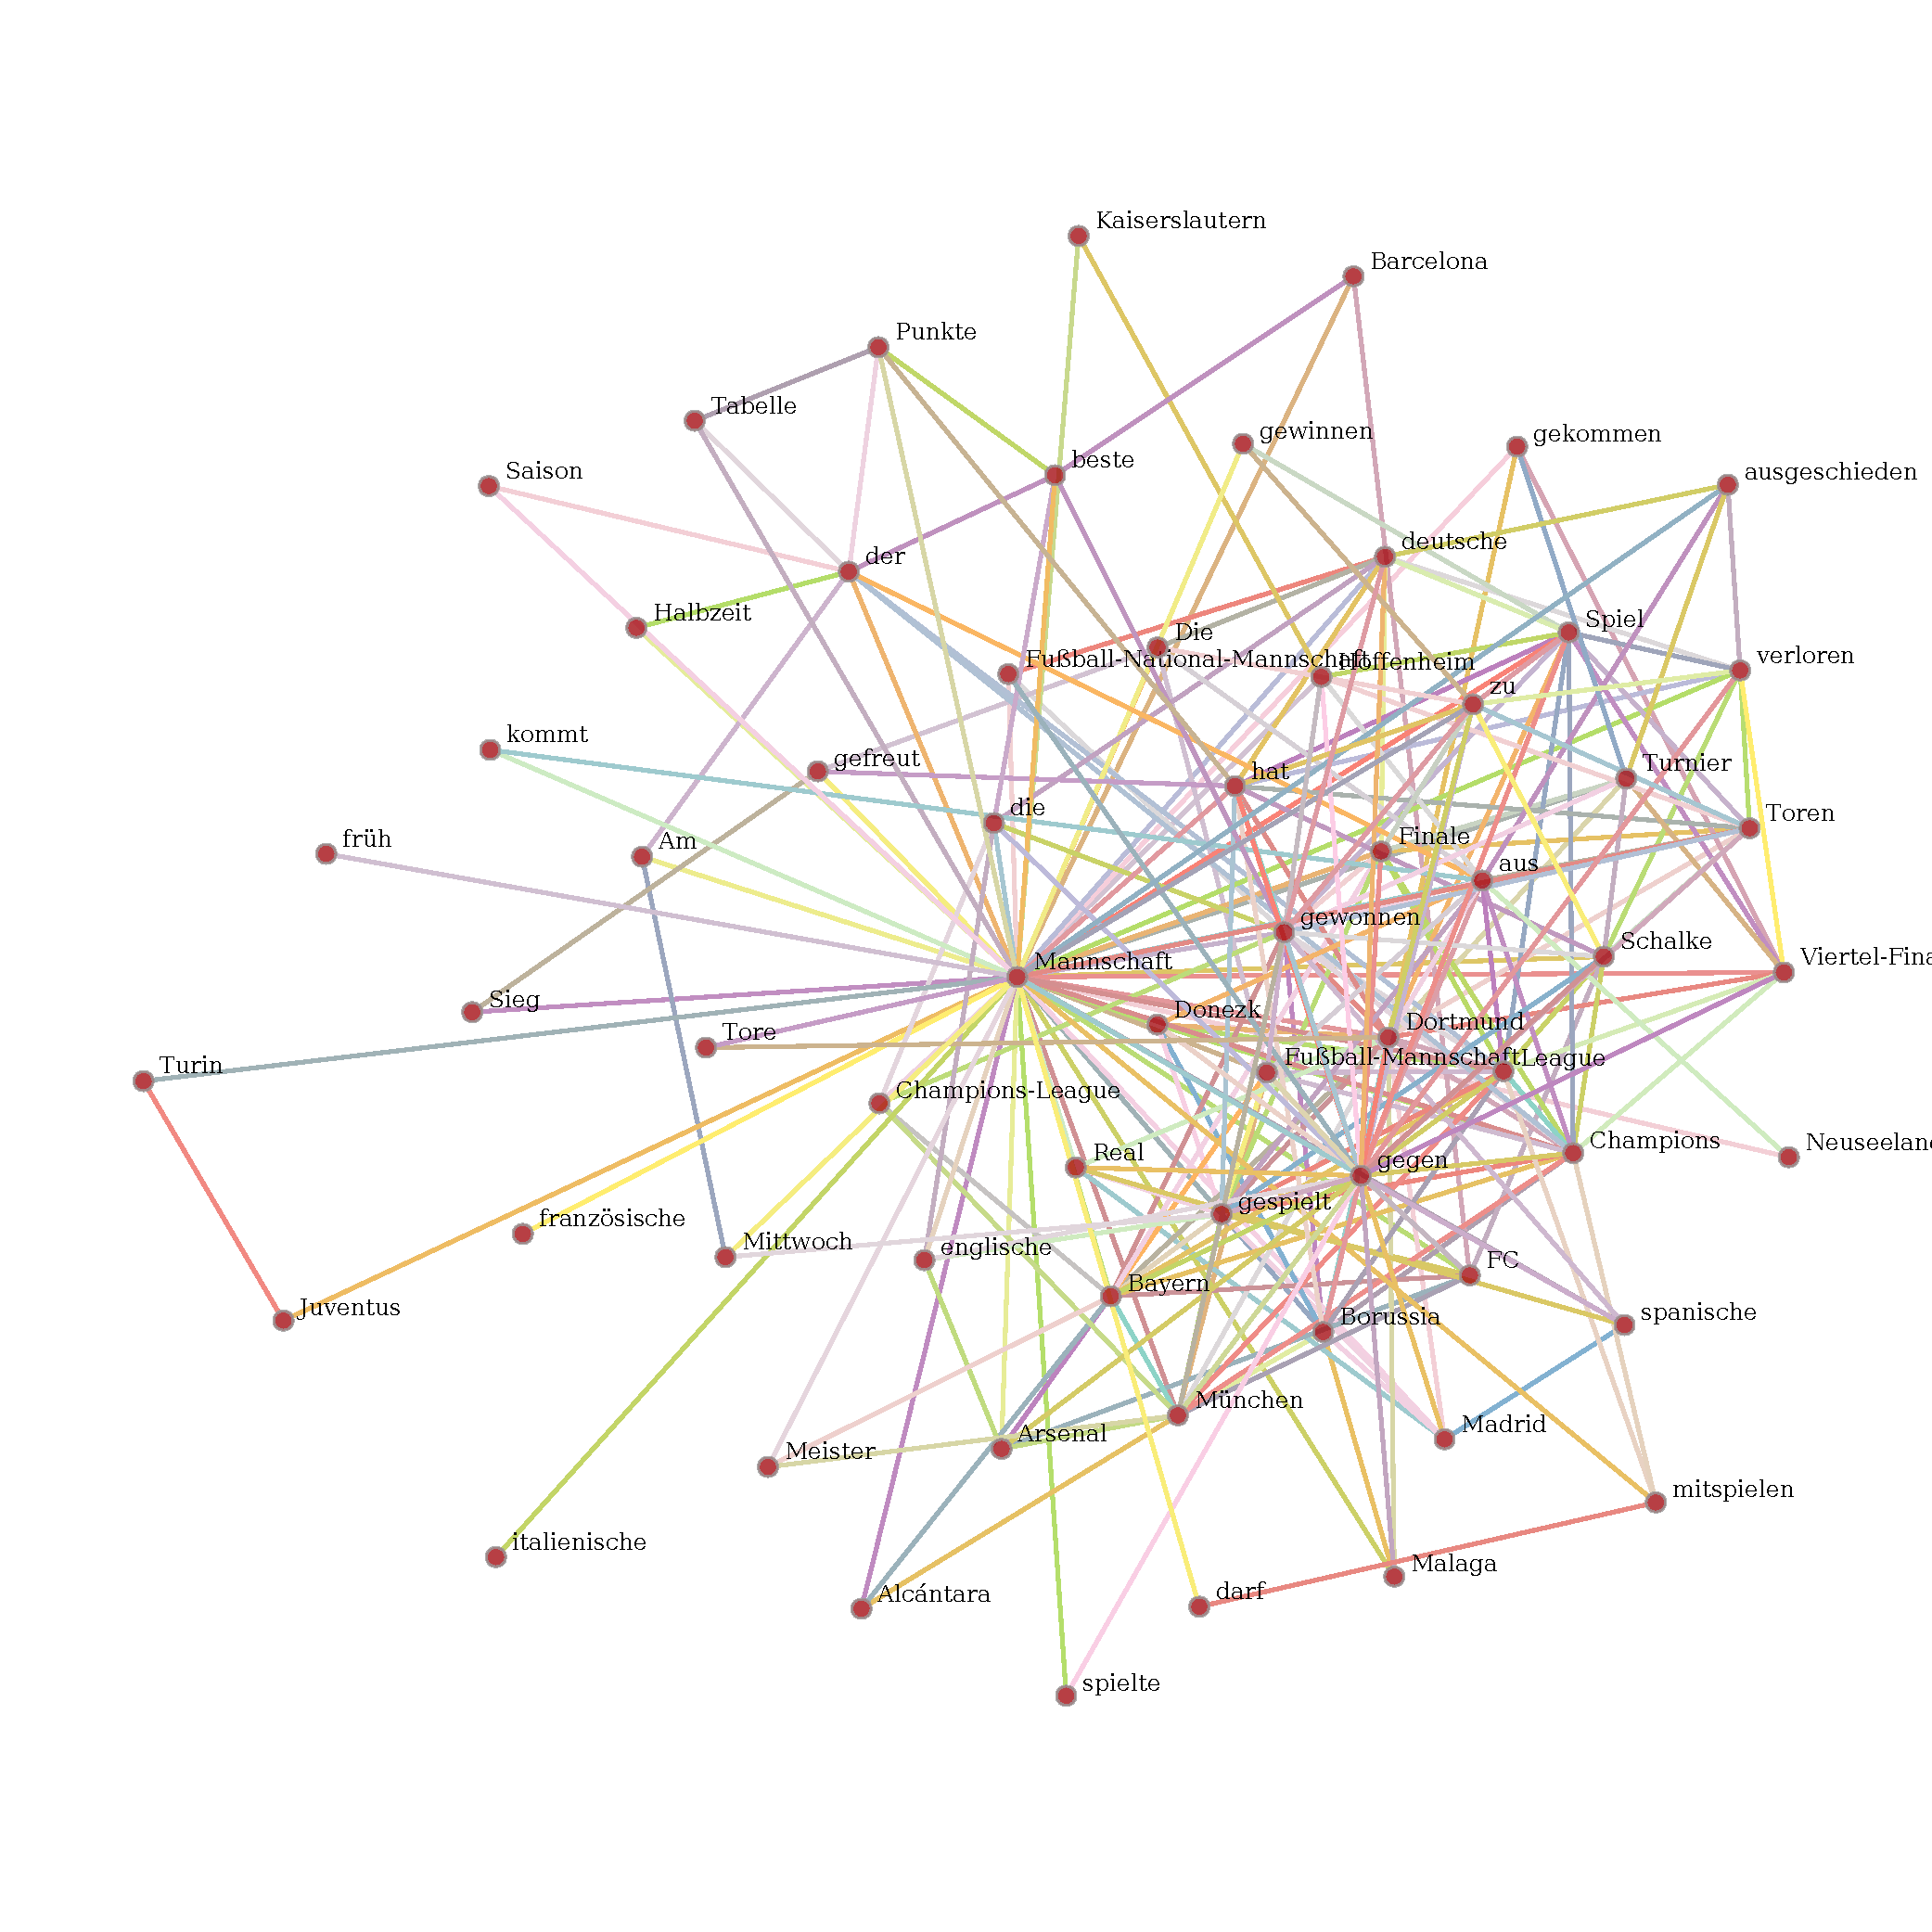
\includegraphics[scale=.4]{../../data/results/cooc_nl/topwords/graph_Mannschaft.pdf}
    \caption{Kookkurrenzgraph Mannschaft (Distanz 1, Schwellwert 1/12, Häufigkeit 62)}
    \label{fig:hw-mannschaft}
\end{figure}

%\begin{figure}[hp!]
%    \centering
%        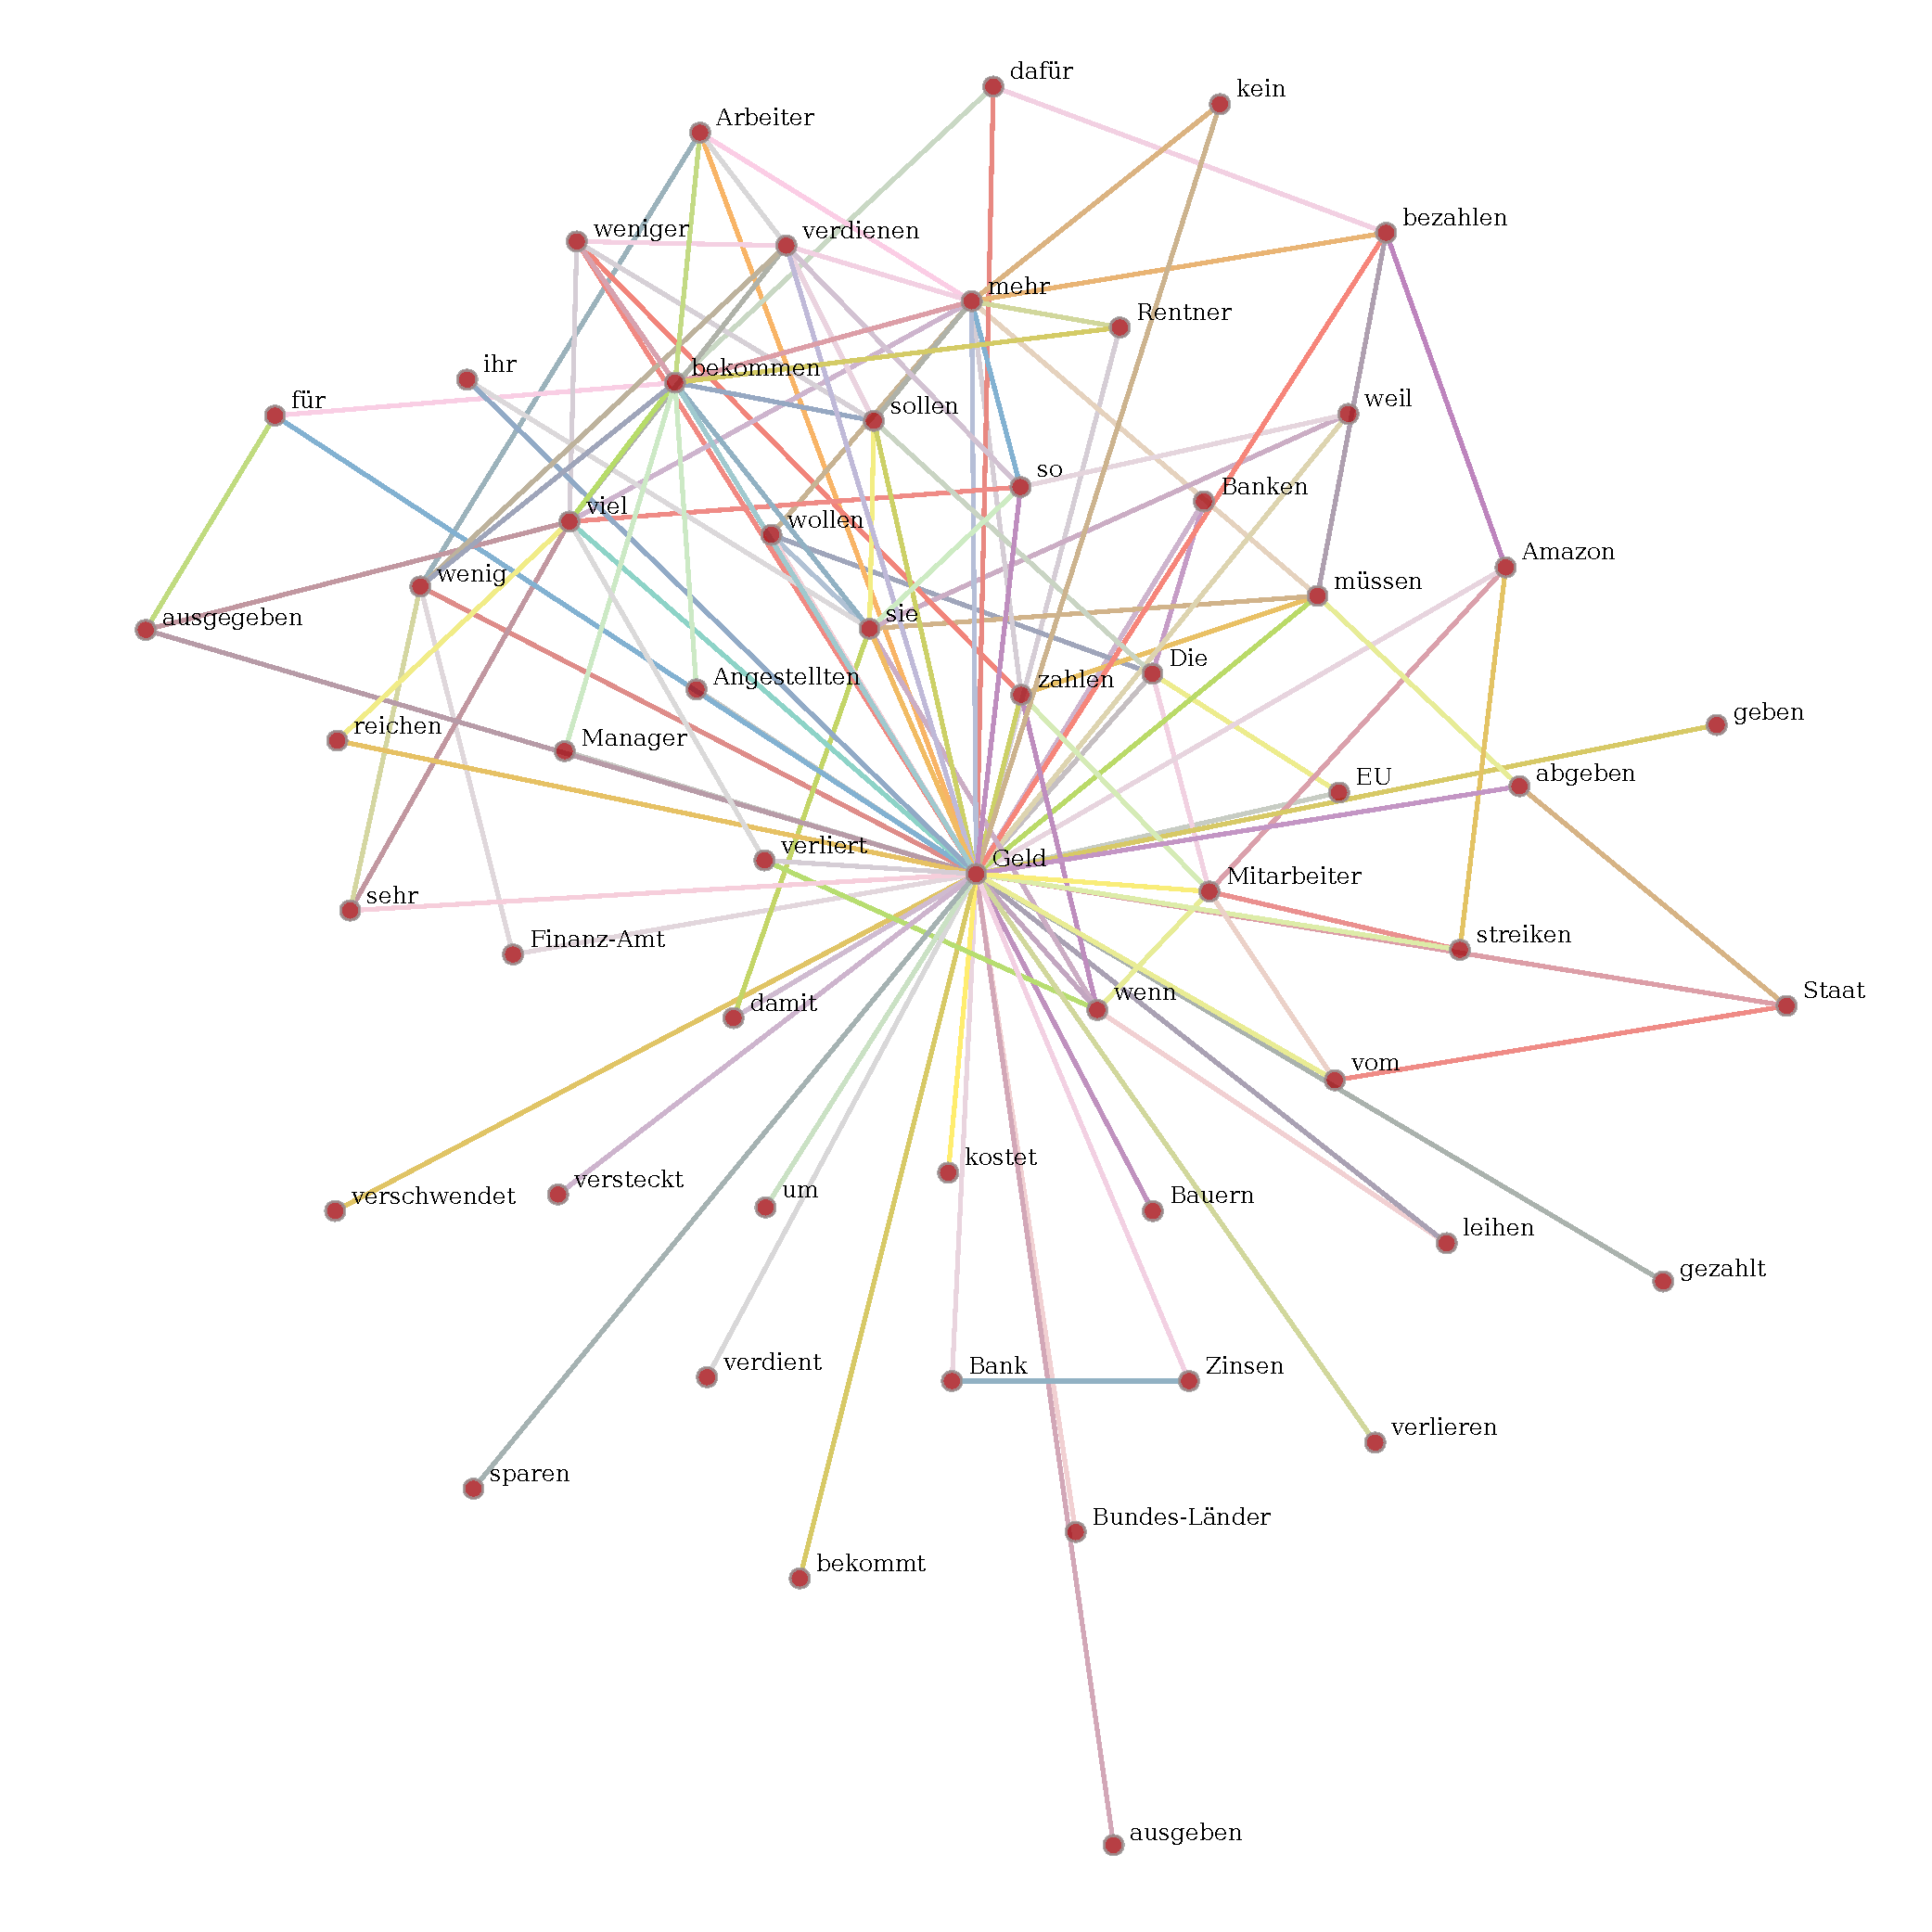
\includegraphics[scale=.4]{../../data/results/cooc_nl/topwords/graph_Geld.pdf}
%    \caption{Kookkurrenzgraph Geld (Distanz 1, Schwellwert 1/12, Häufigkeit 54)}
%    \label{fig:hw-geld}
%\end{figure}

\begin{figure}[hp!]
    \centering
        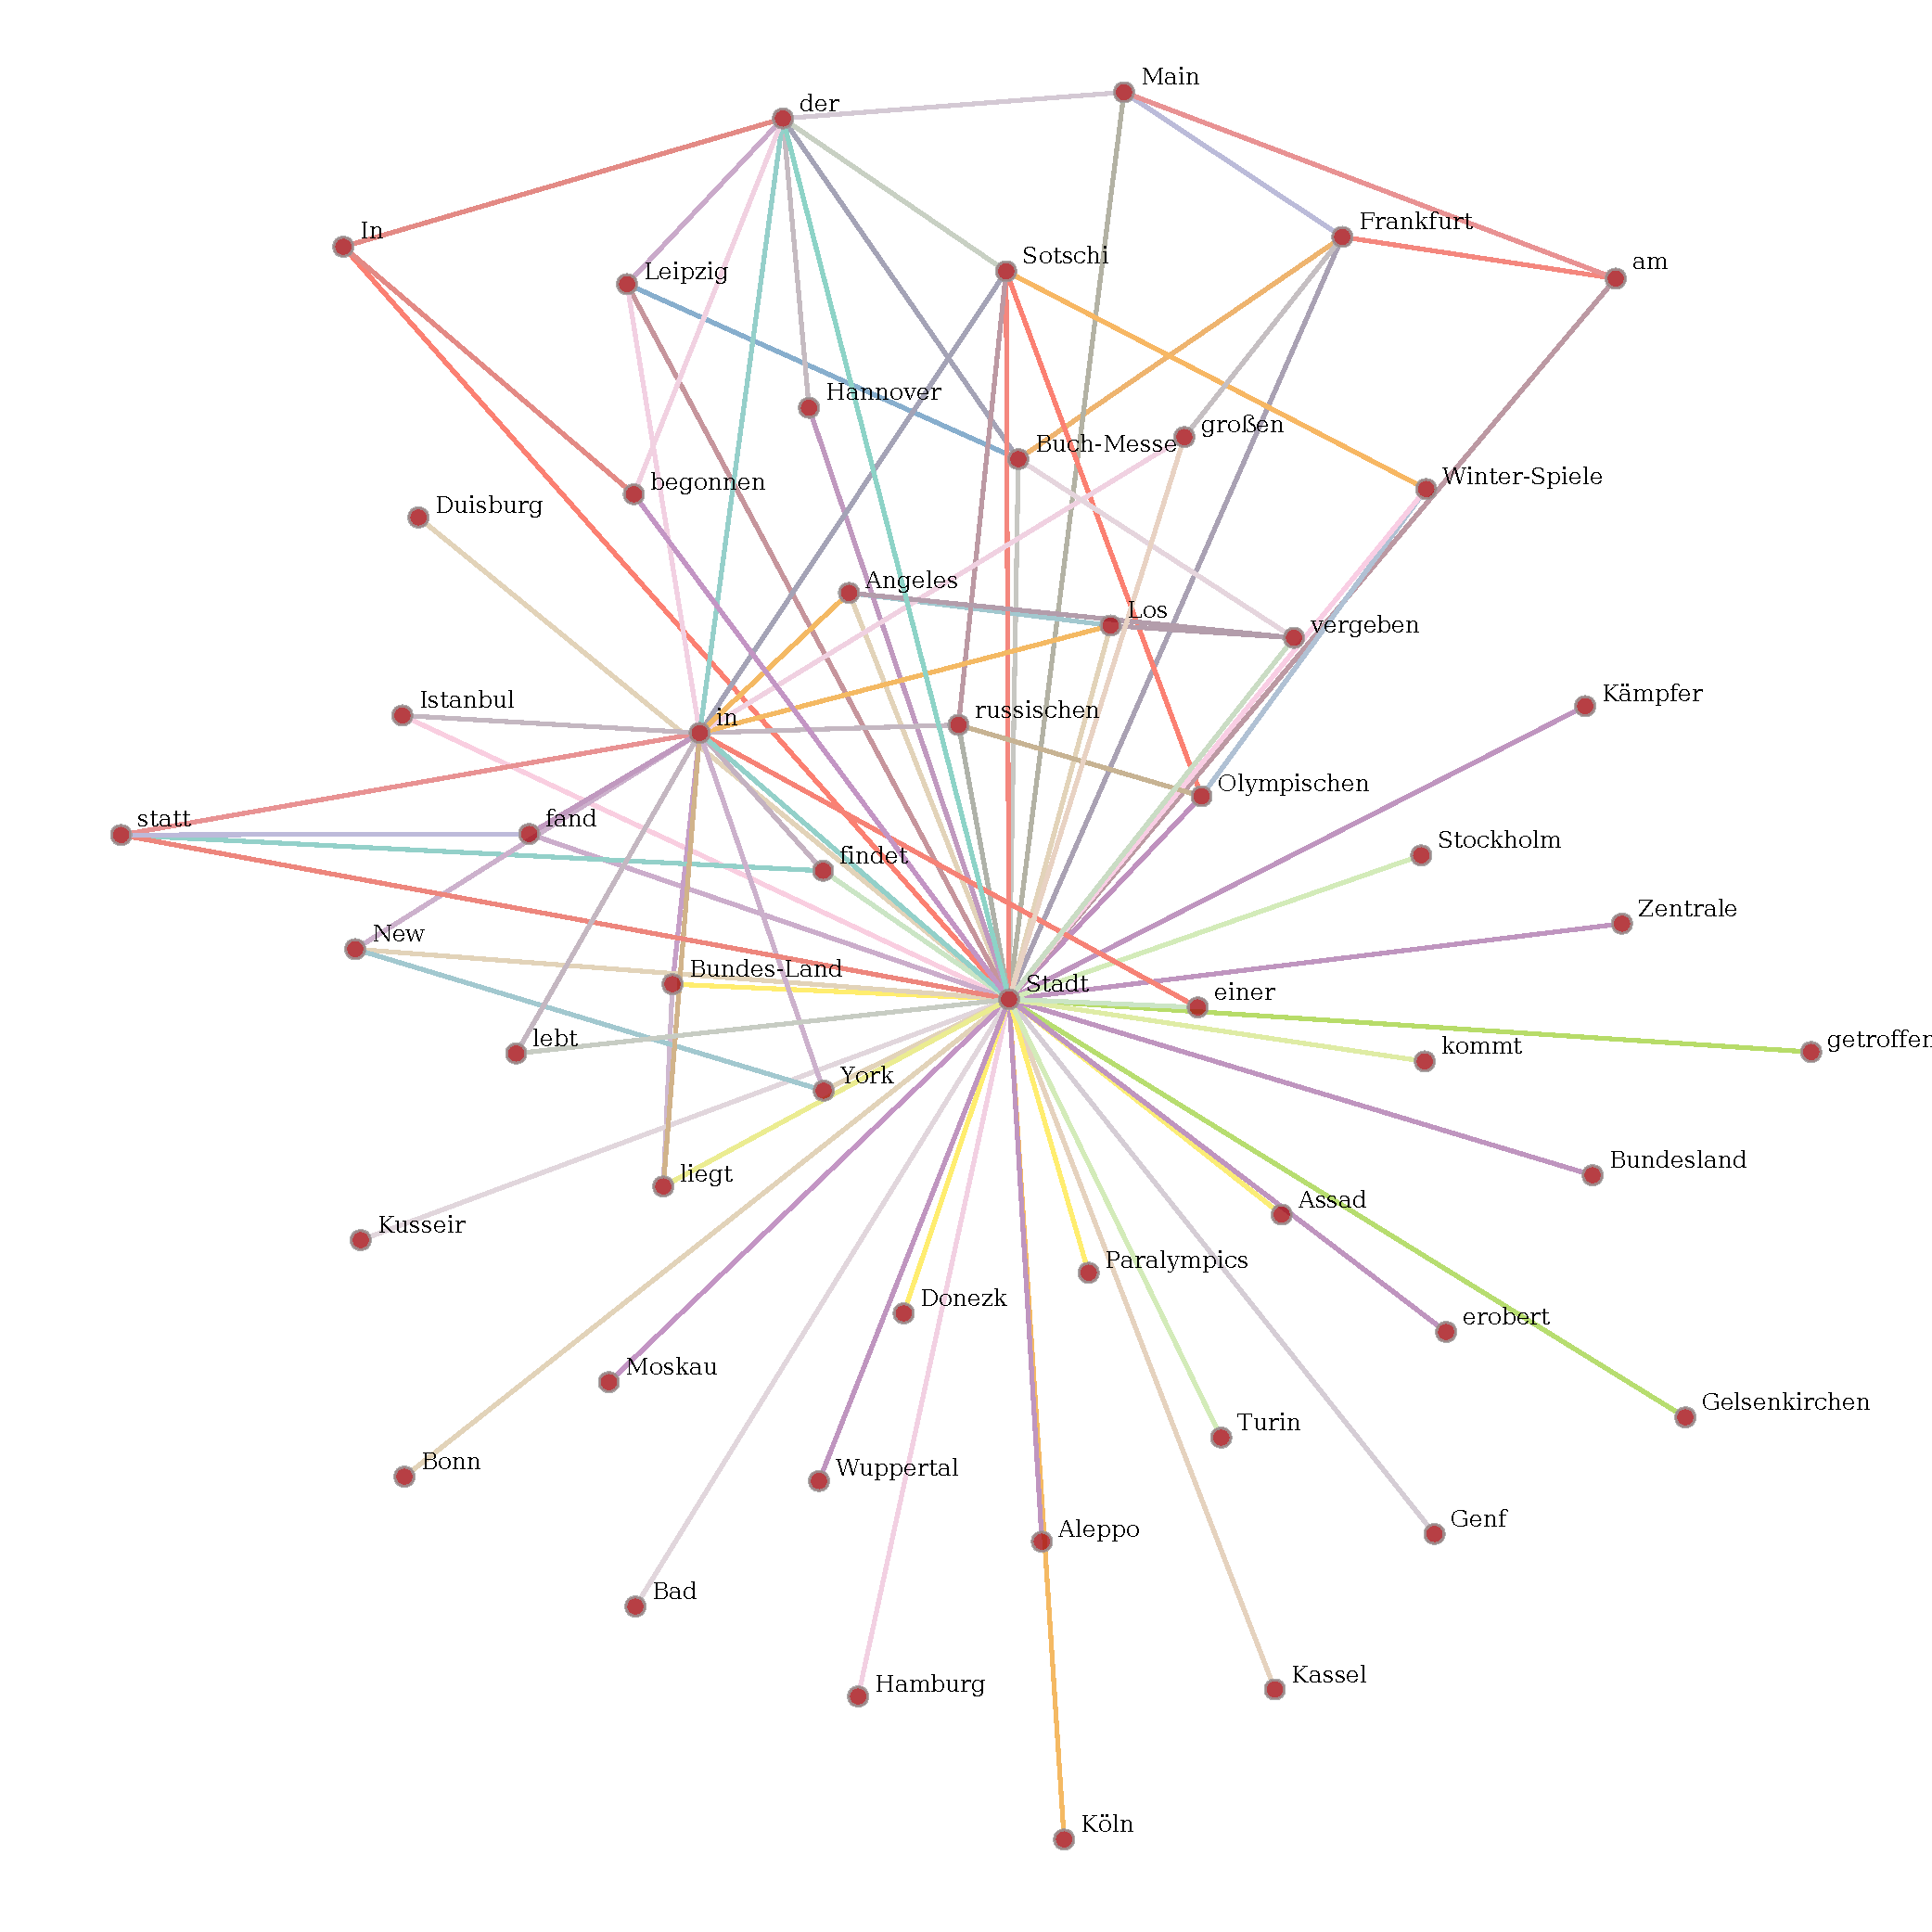
\includegraphics[scale=.4]{../../data/results/cooc_nl/topwords/graph_Stadt.pdf}
    \caption{Kookkurrenzgraph Stadt (Distanz 1, Schwellwert 1/12, Häufigkeit 51)}
    \label{fig:hw-stadt}
\end{figure}

\begin{figure}[hp!]
    \centering
        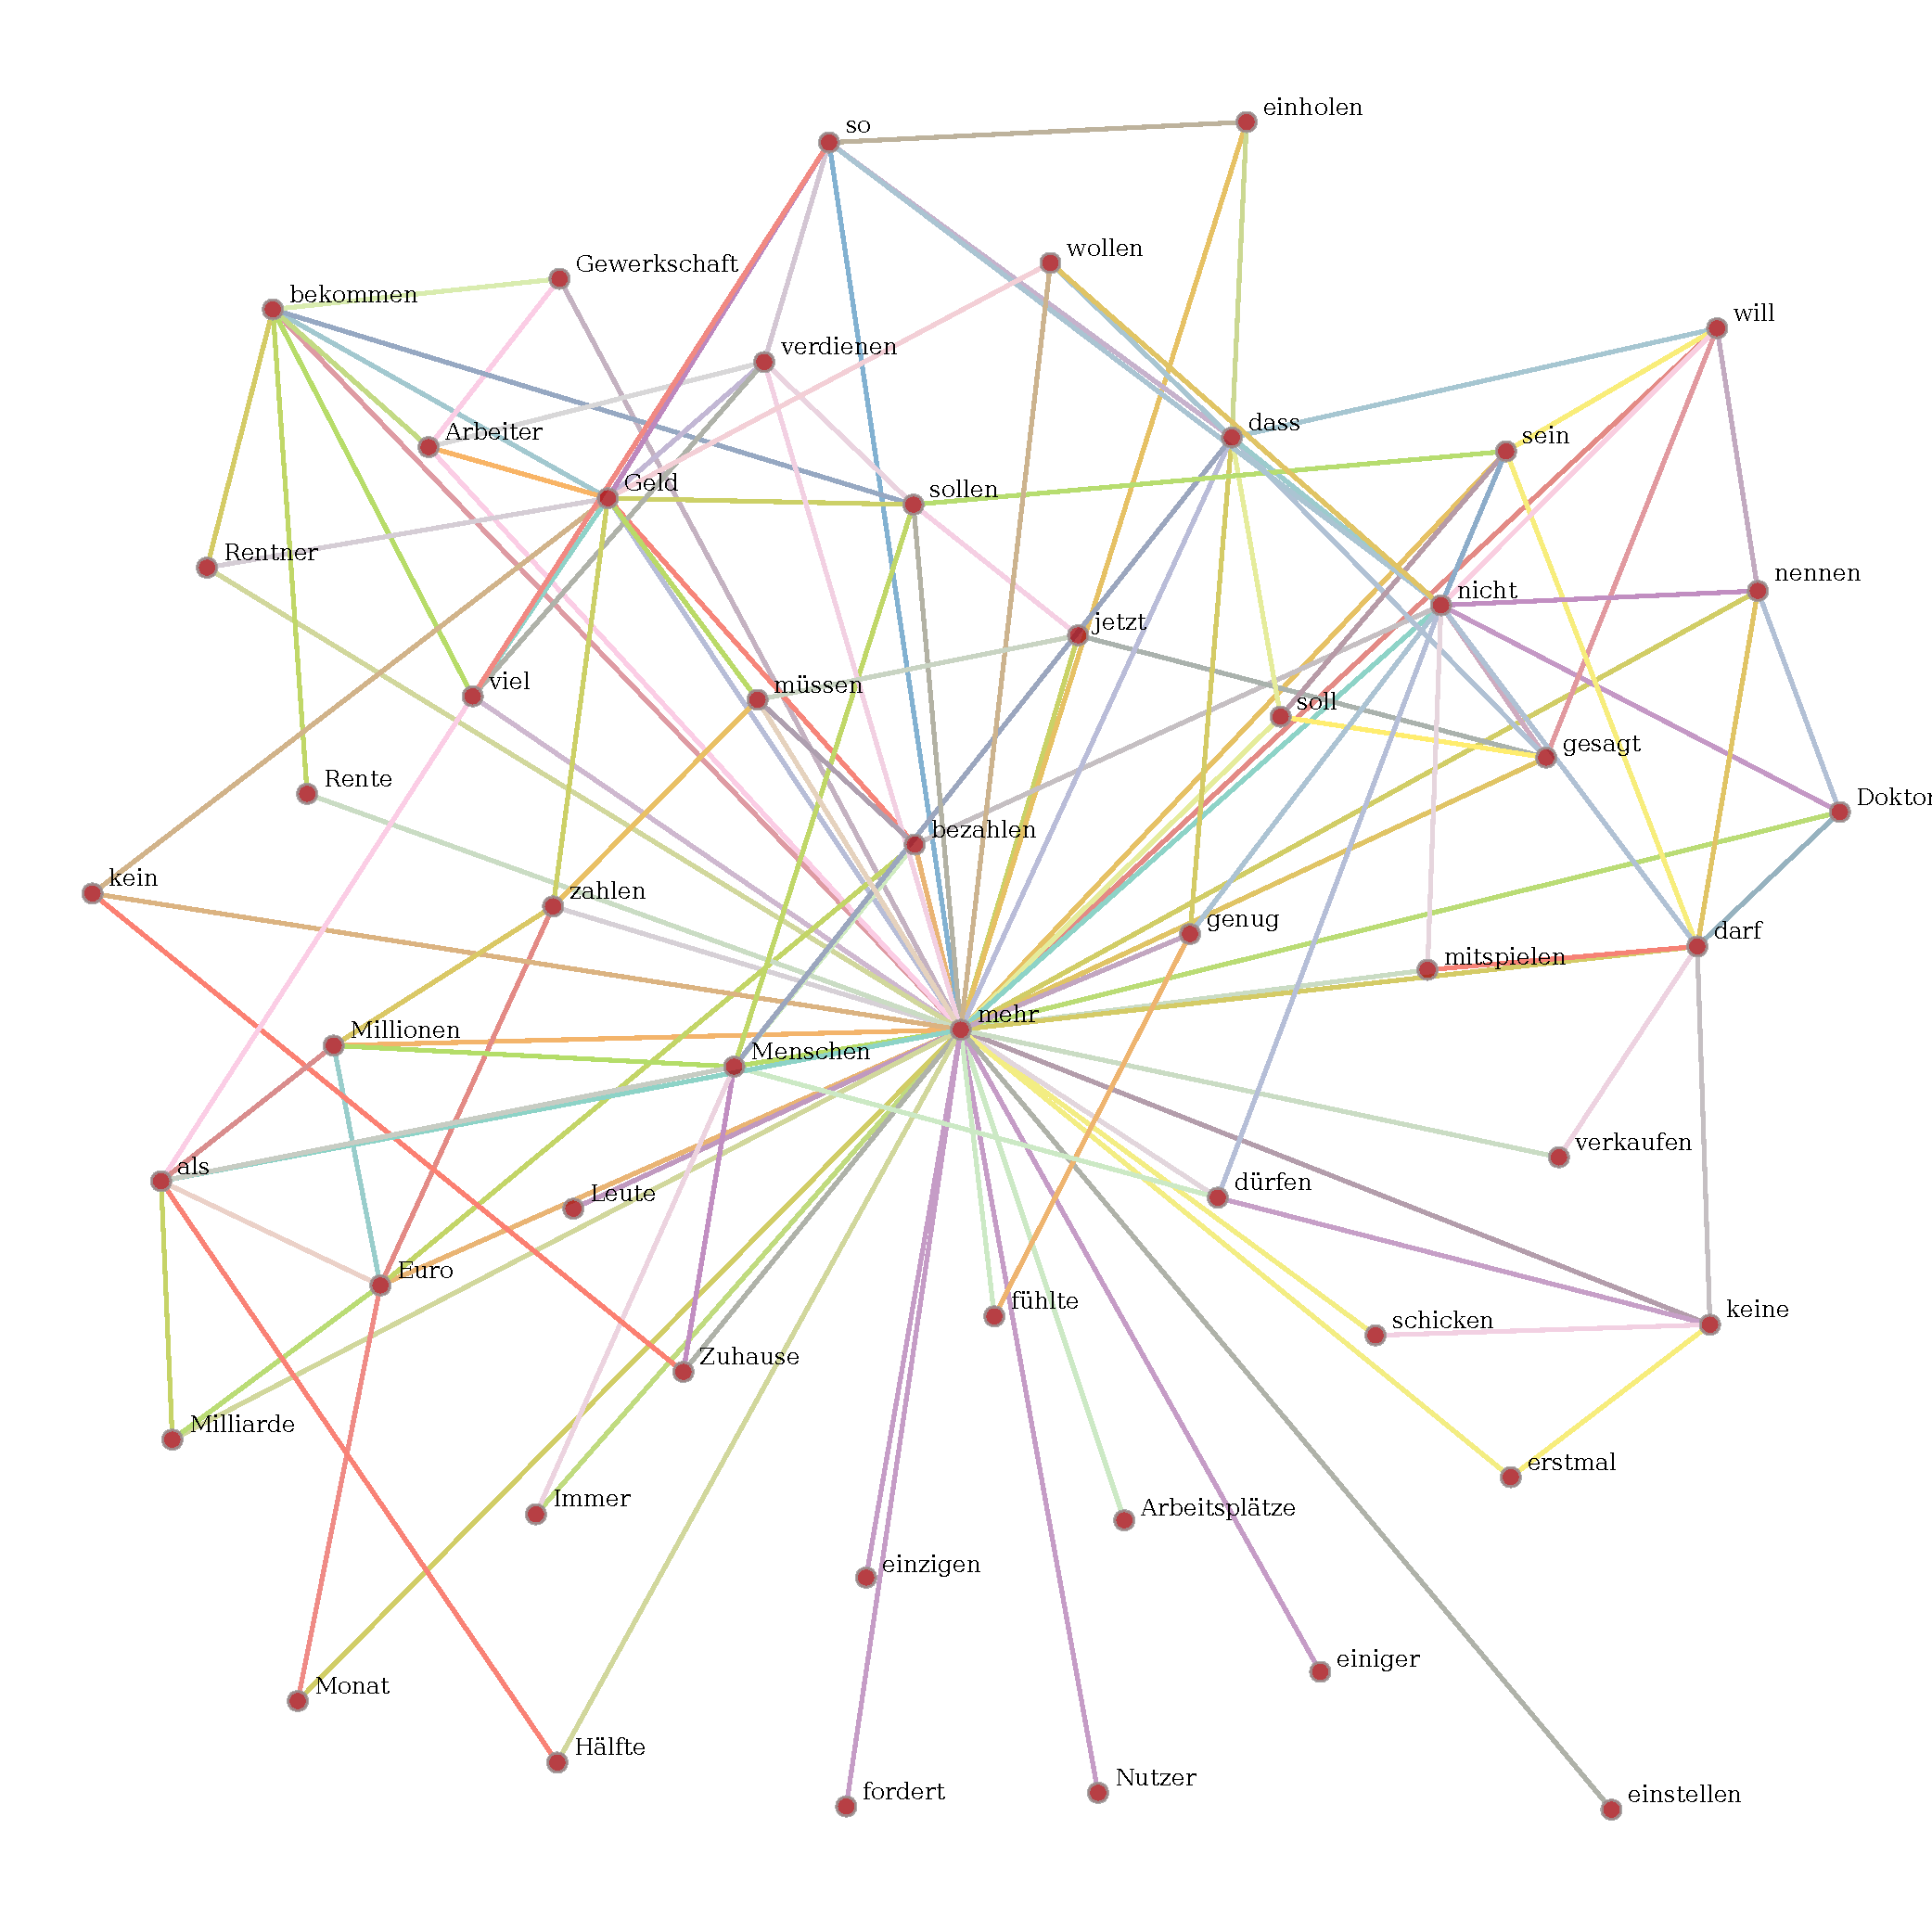
\includegraphics[scale=.4]{../../data/results/cooc_nl/topwords/graph_mehr.pdf}
    \caption{Kookkurrenzgraph mehr (Distanz 1, Schwellwert 1/12, Häufigkeit 50)}
    \label{fig:hw-mehr}
\end{figure}


\pagebreak
\subsubsection{deunews2010\_10K}

\begin{figure}[hp!]
    \centering
        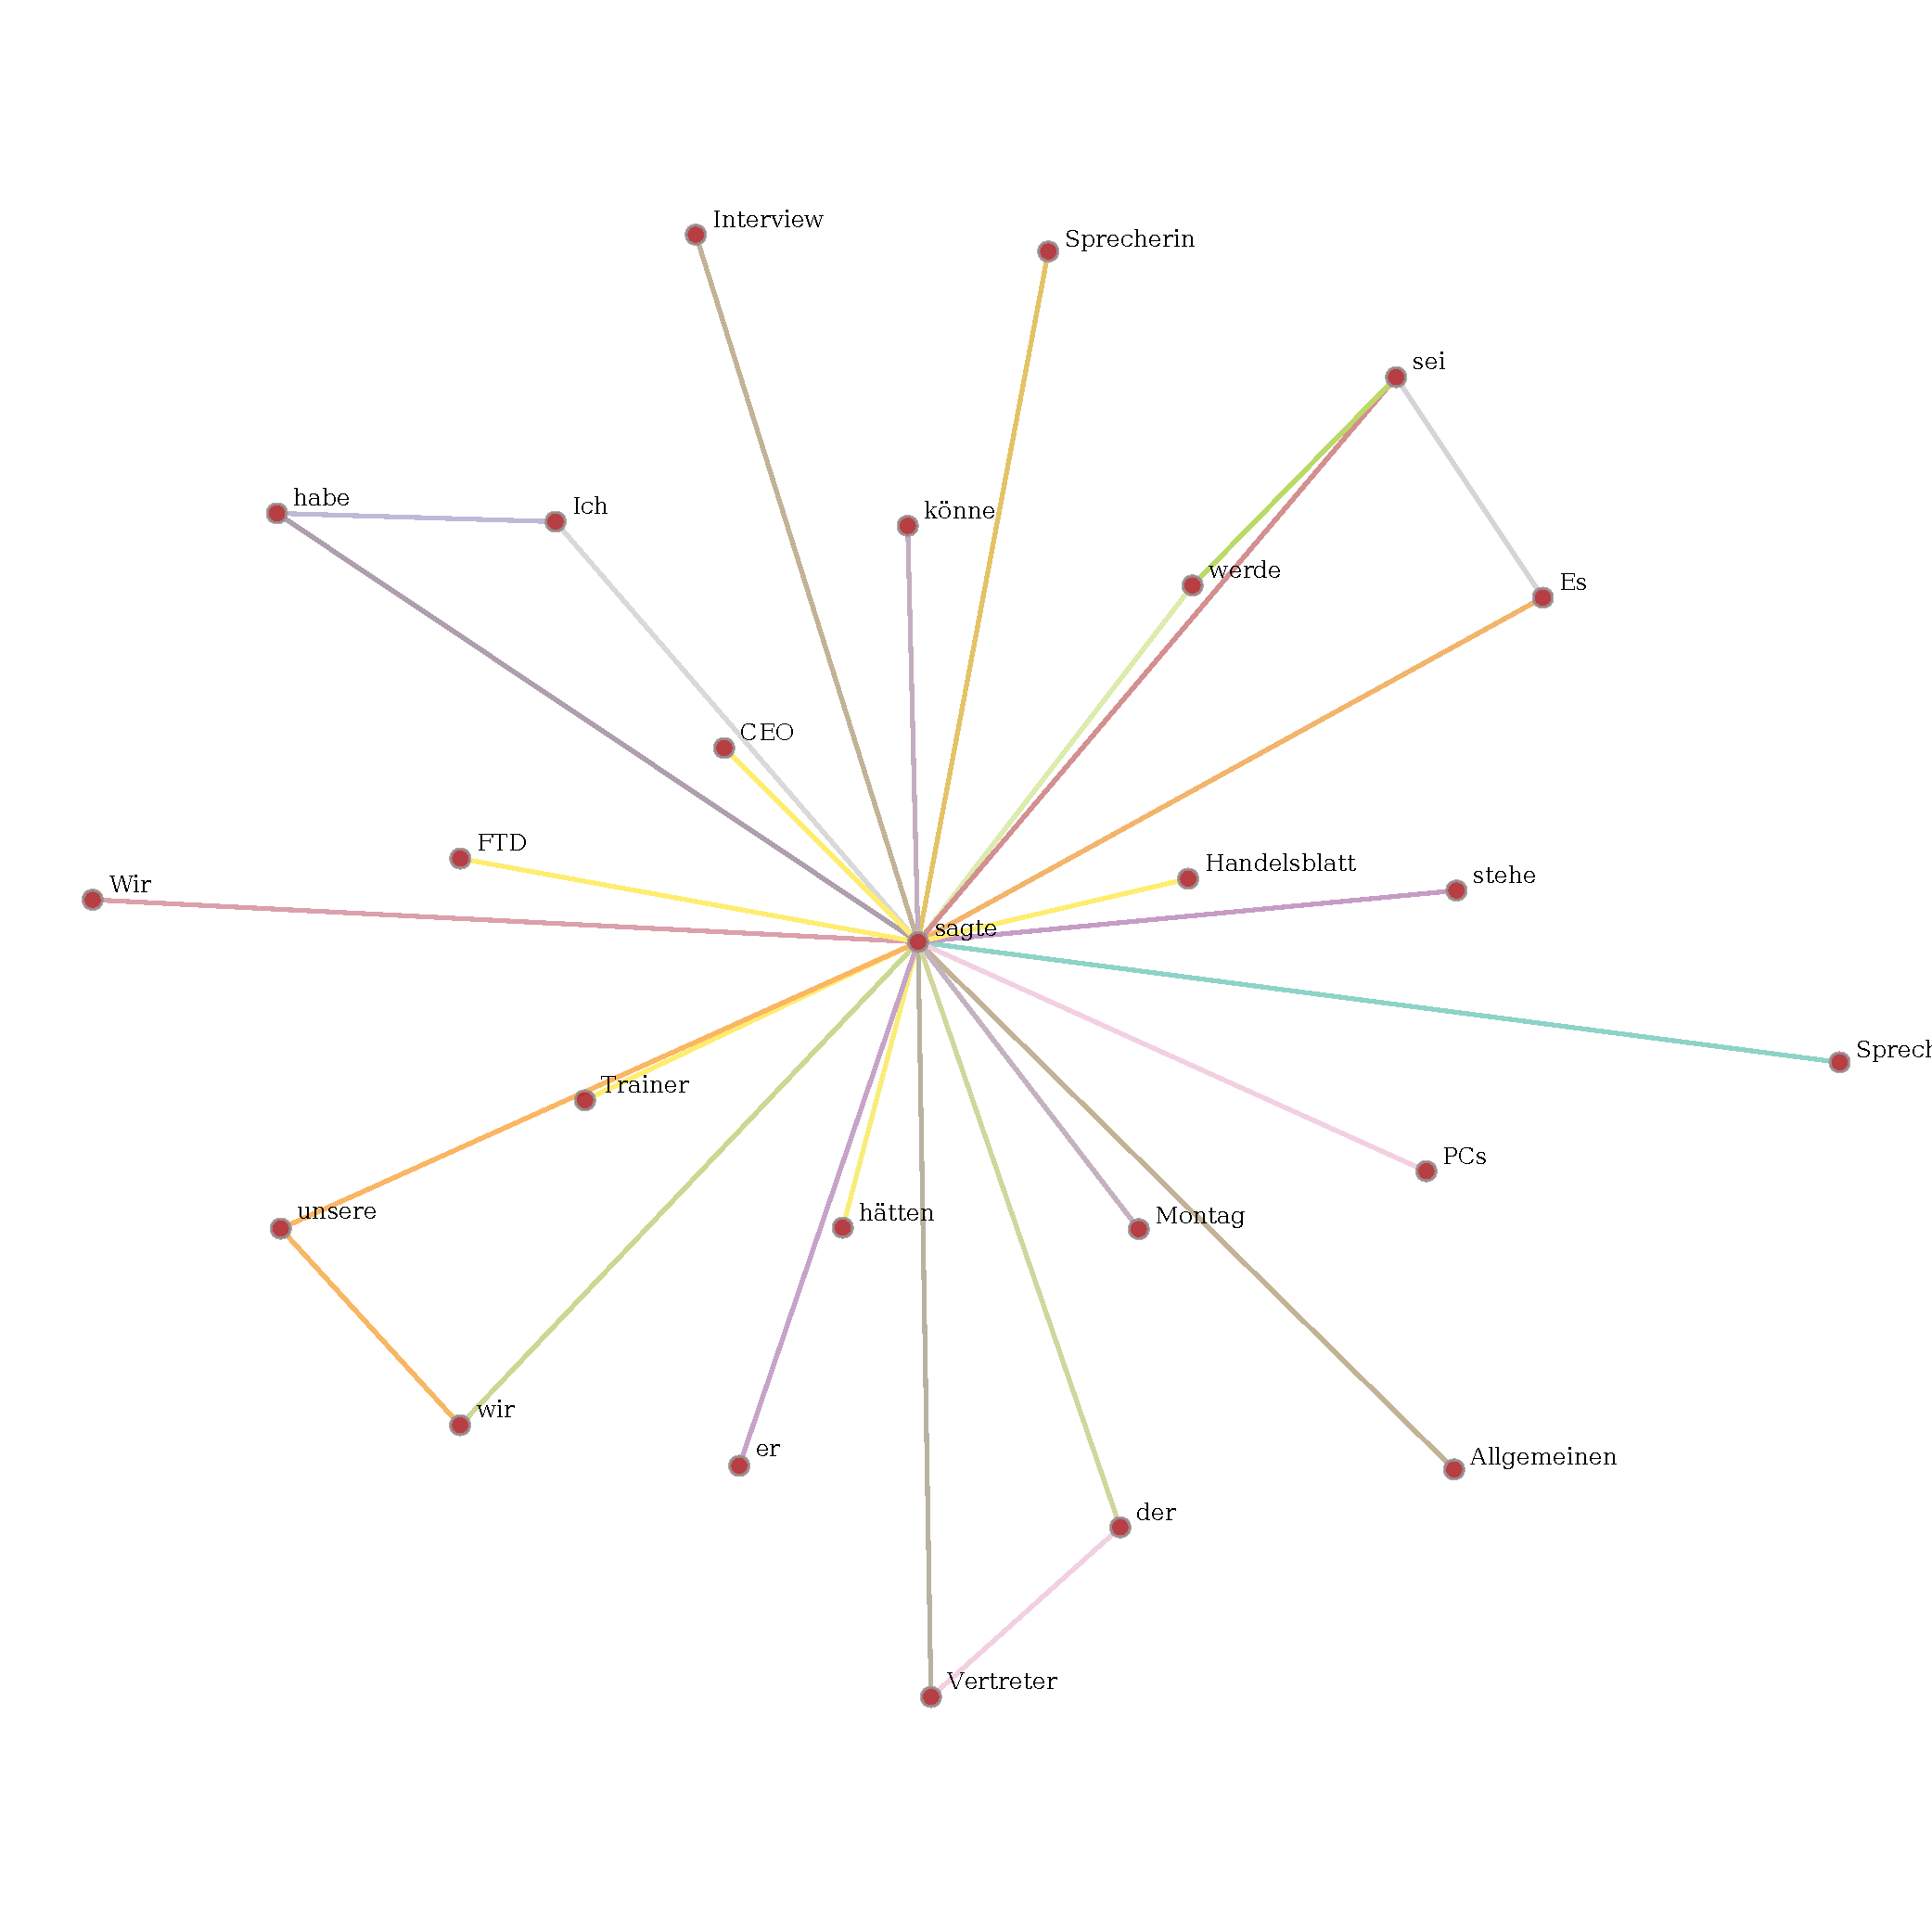
\includegraphics[scale=.4]{../../data/results/cooc_denews10k/topwords/graph_sagte.pdf}
    \caption{Kookkurrenzgraph sagte (Distanz 1, Schwellwert 1/12, Häufigkeit 24)}
    \label{fig:hw-sagte}
\end{figure}

\begin{figure}[hp!]
    \centering
        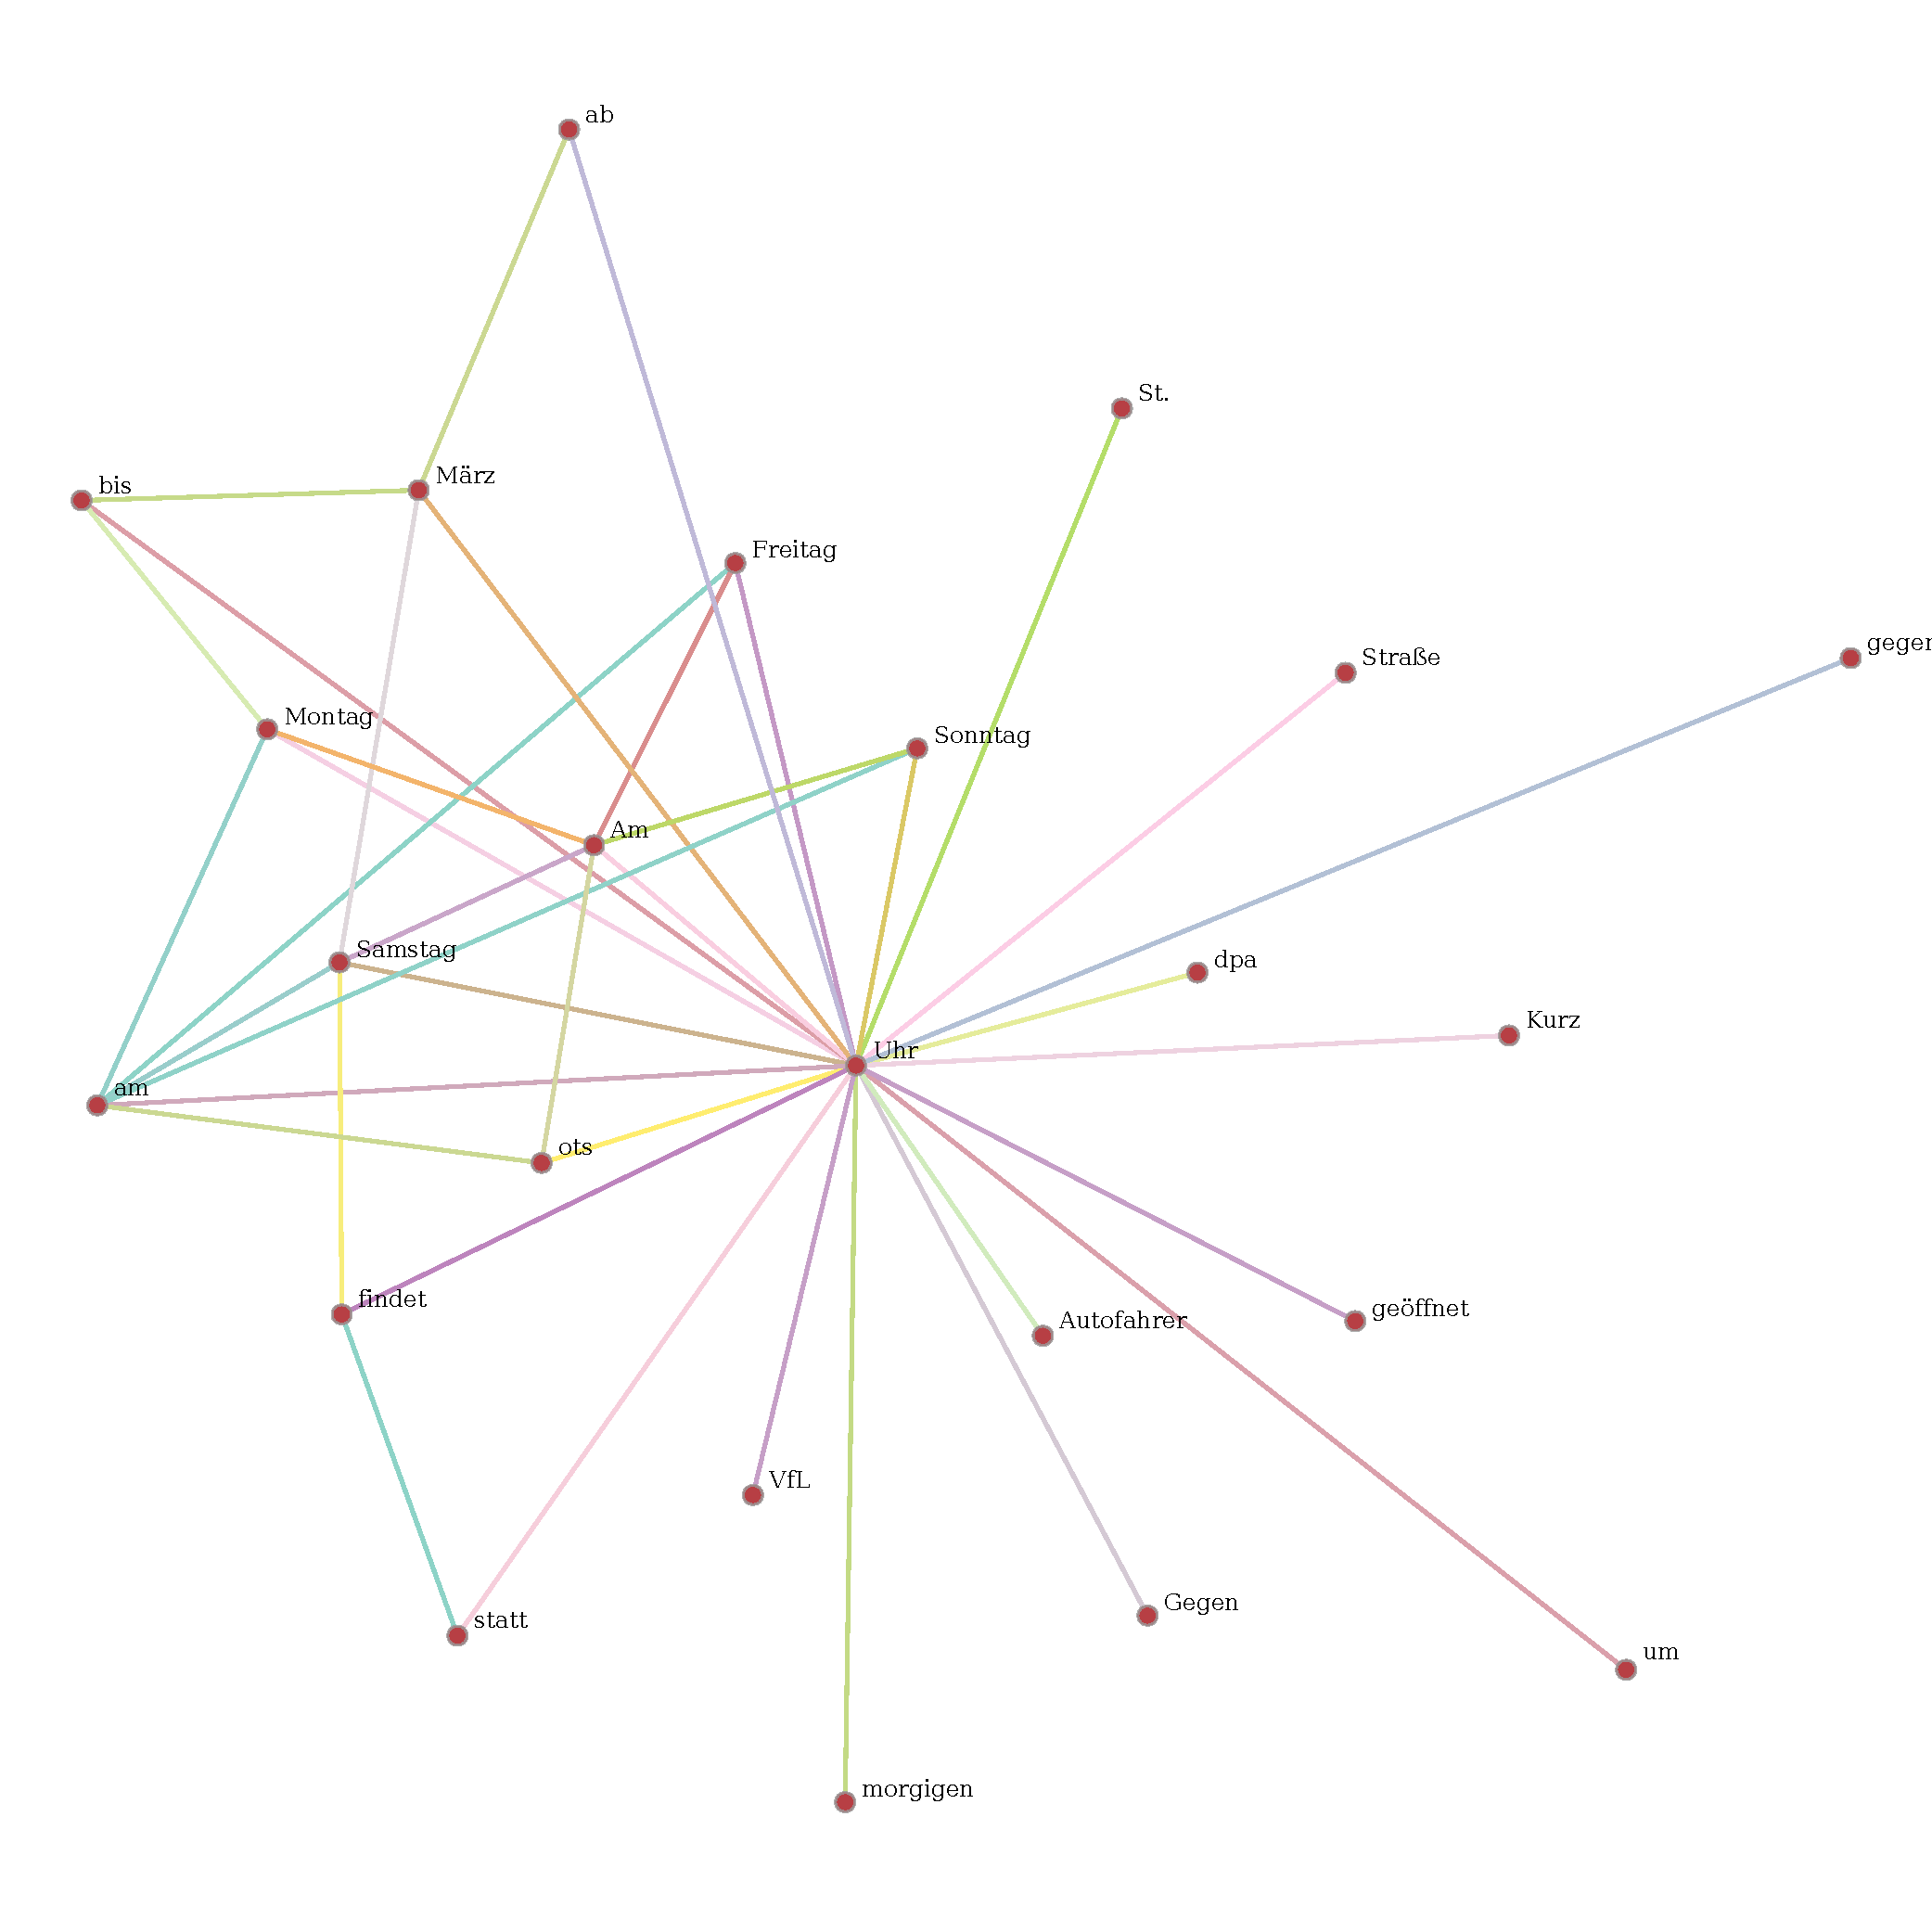
\includegraphics[scale=.4]{../../data/results/cooc_denews10k/topwords/graph_Uhr.pdf}
    \caption{Kookkurrenzgraph Uhr (Distanz 1, Schwellwert 1/12, Häufigkeit 23)}
    \label{fig:hw-uhr}
\end{figure}

\begin{figure}[hp!]
    \centering
        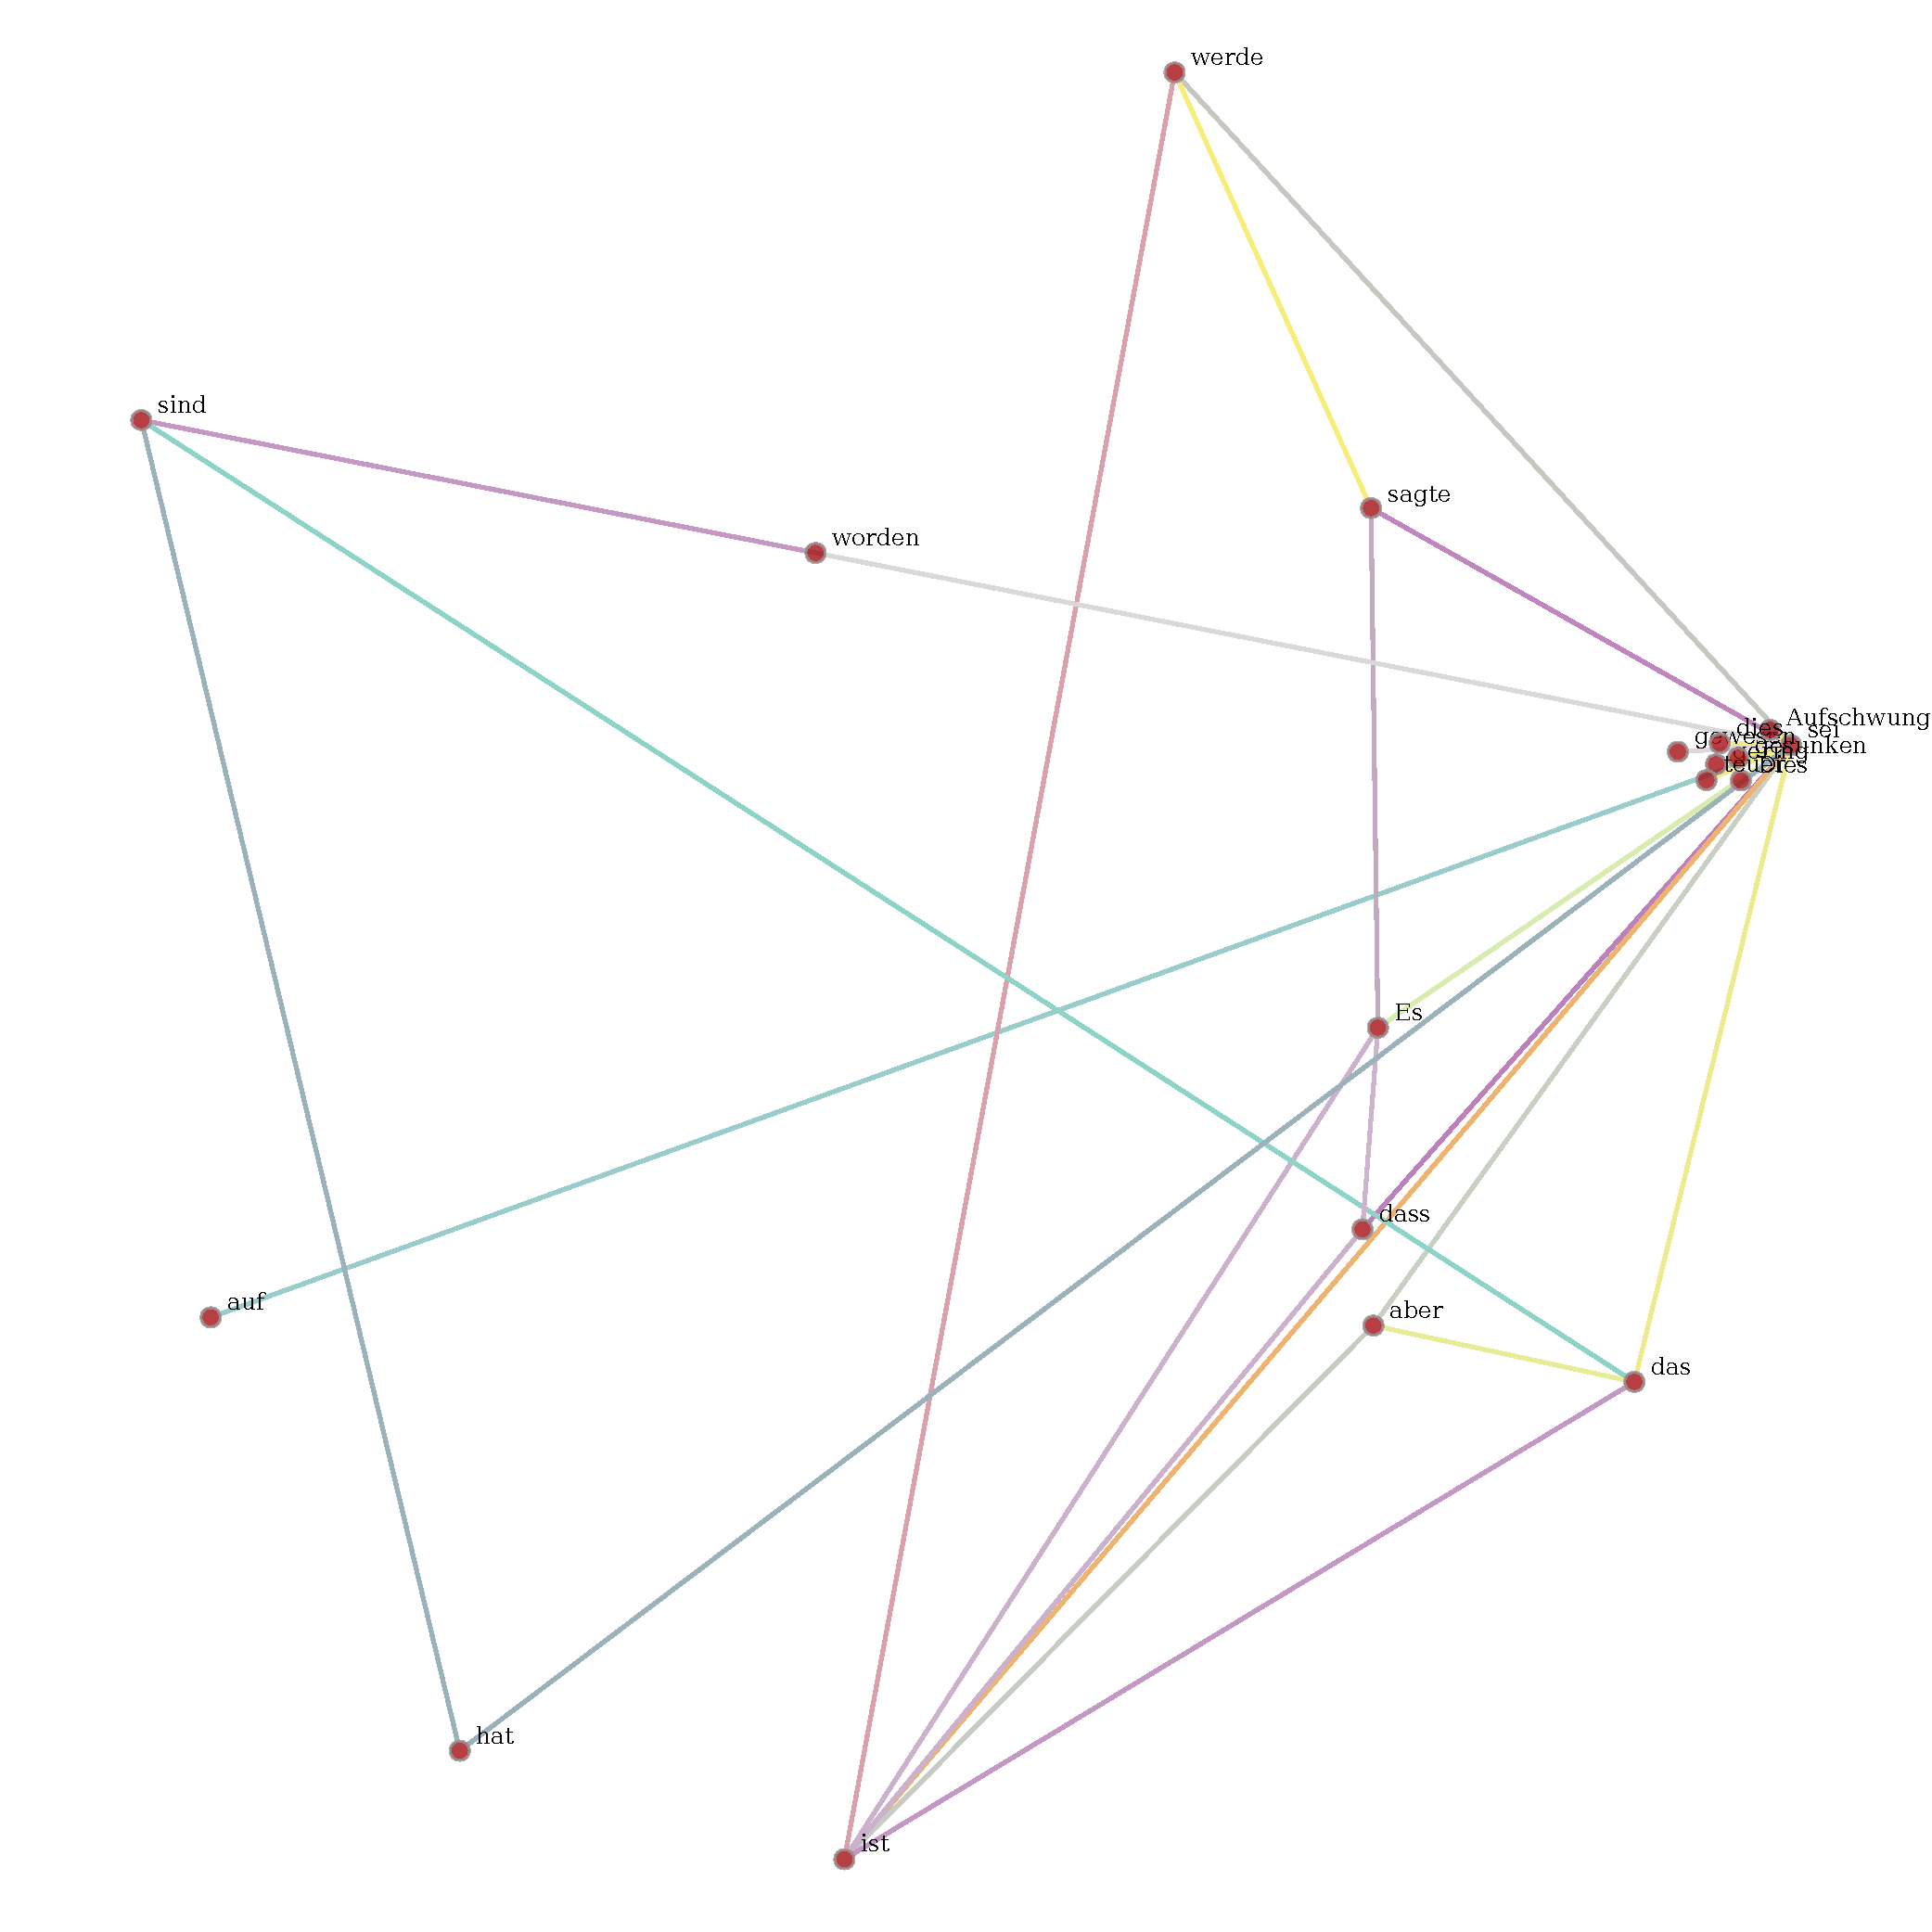
\includegraphics[scale=.4]{../../data/results/cooc_denews10k/topwords/graph_sei.pdf}
    \caption{Kookkurrenzgraph sei (Distanz 1, Schwellwert 1/12, Häufigkeit 18)}
    \label{fig:hw-sei}
\end{figure}

\begin{figure}[hp!]
    \centering
        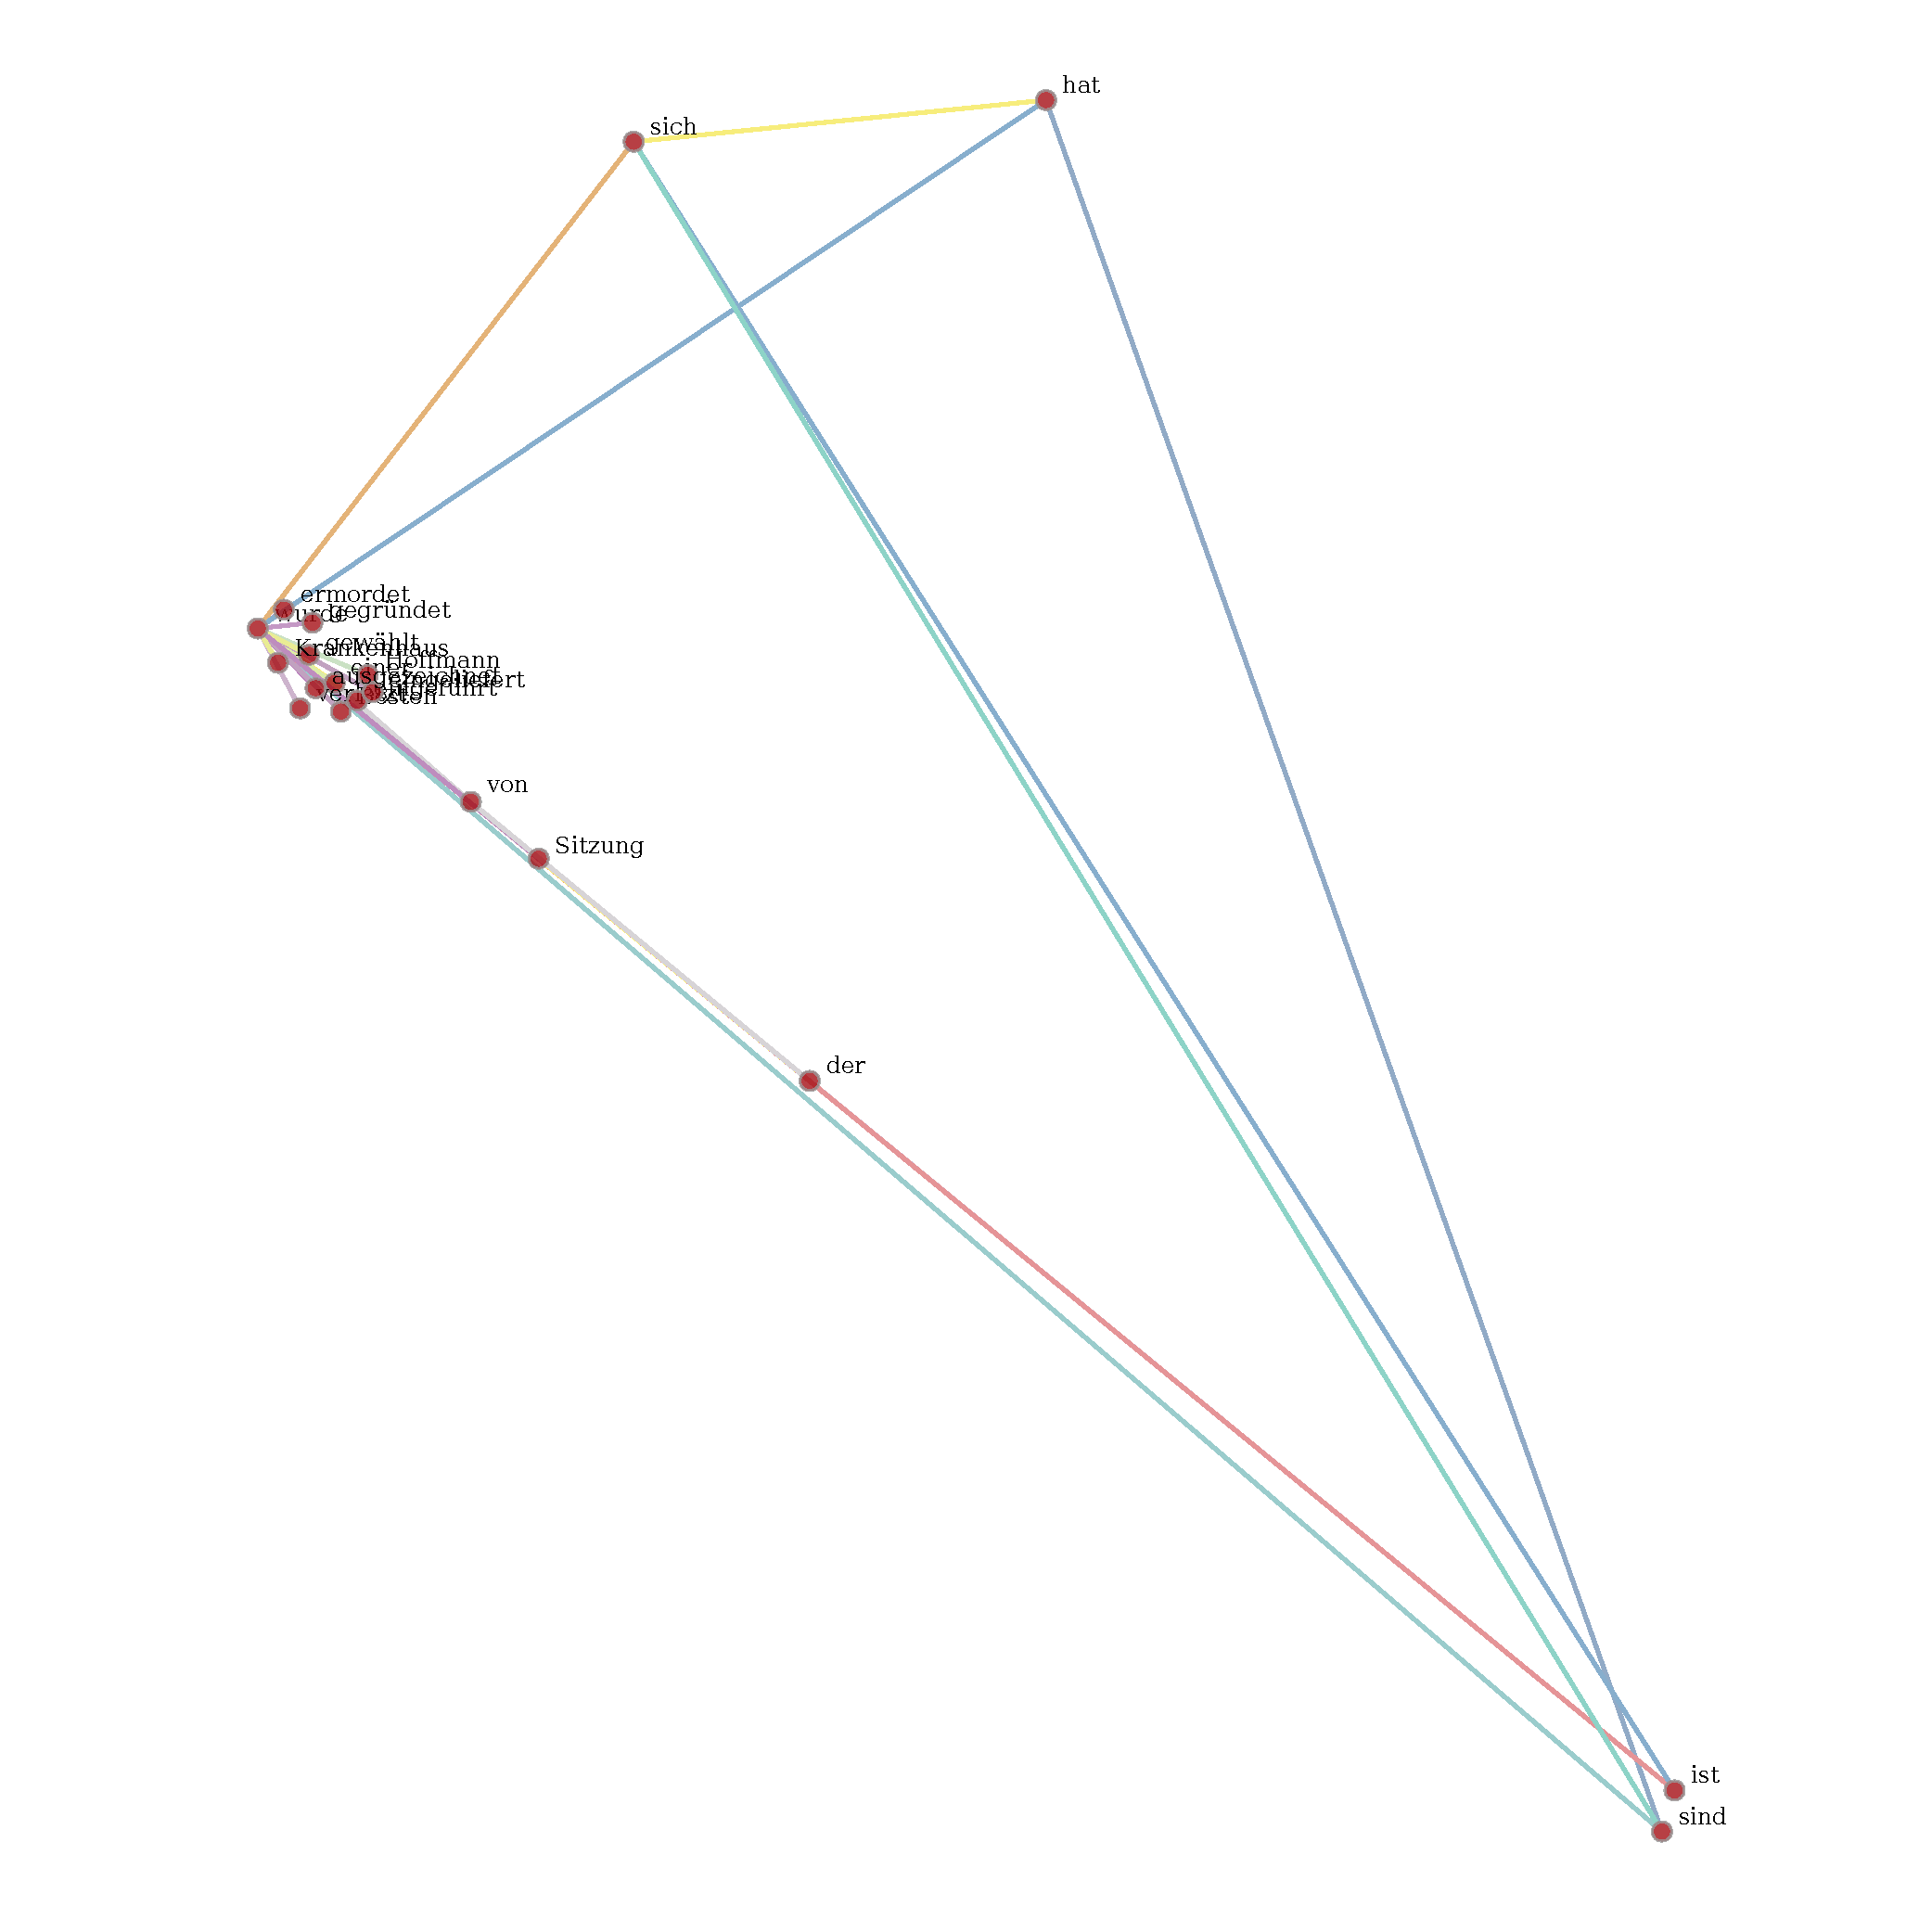
\includegraphics[scale=.4]{../../data/results/cooc_denews10k/topwords/graph_wurde.pdf}
    \caption{Kookkurrenzgraph wurde (Distanz 1, Schwellwert 1/12, Häufigkeit 24)}
    \label{fig:hw-wurde}
\end{figure}

\begin{figure}[hp!]
    \centering
        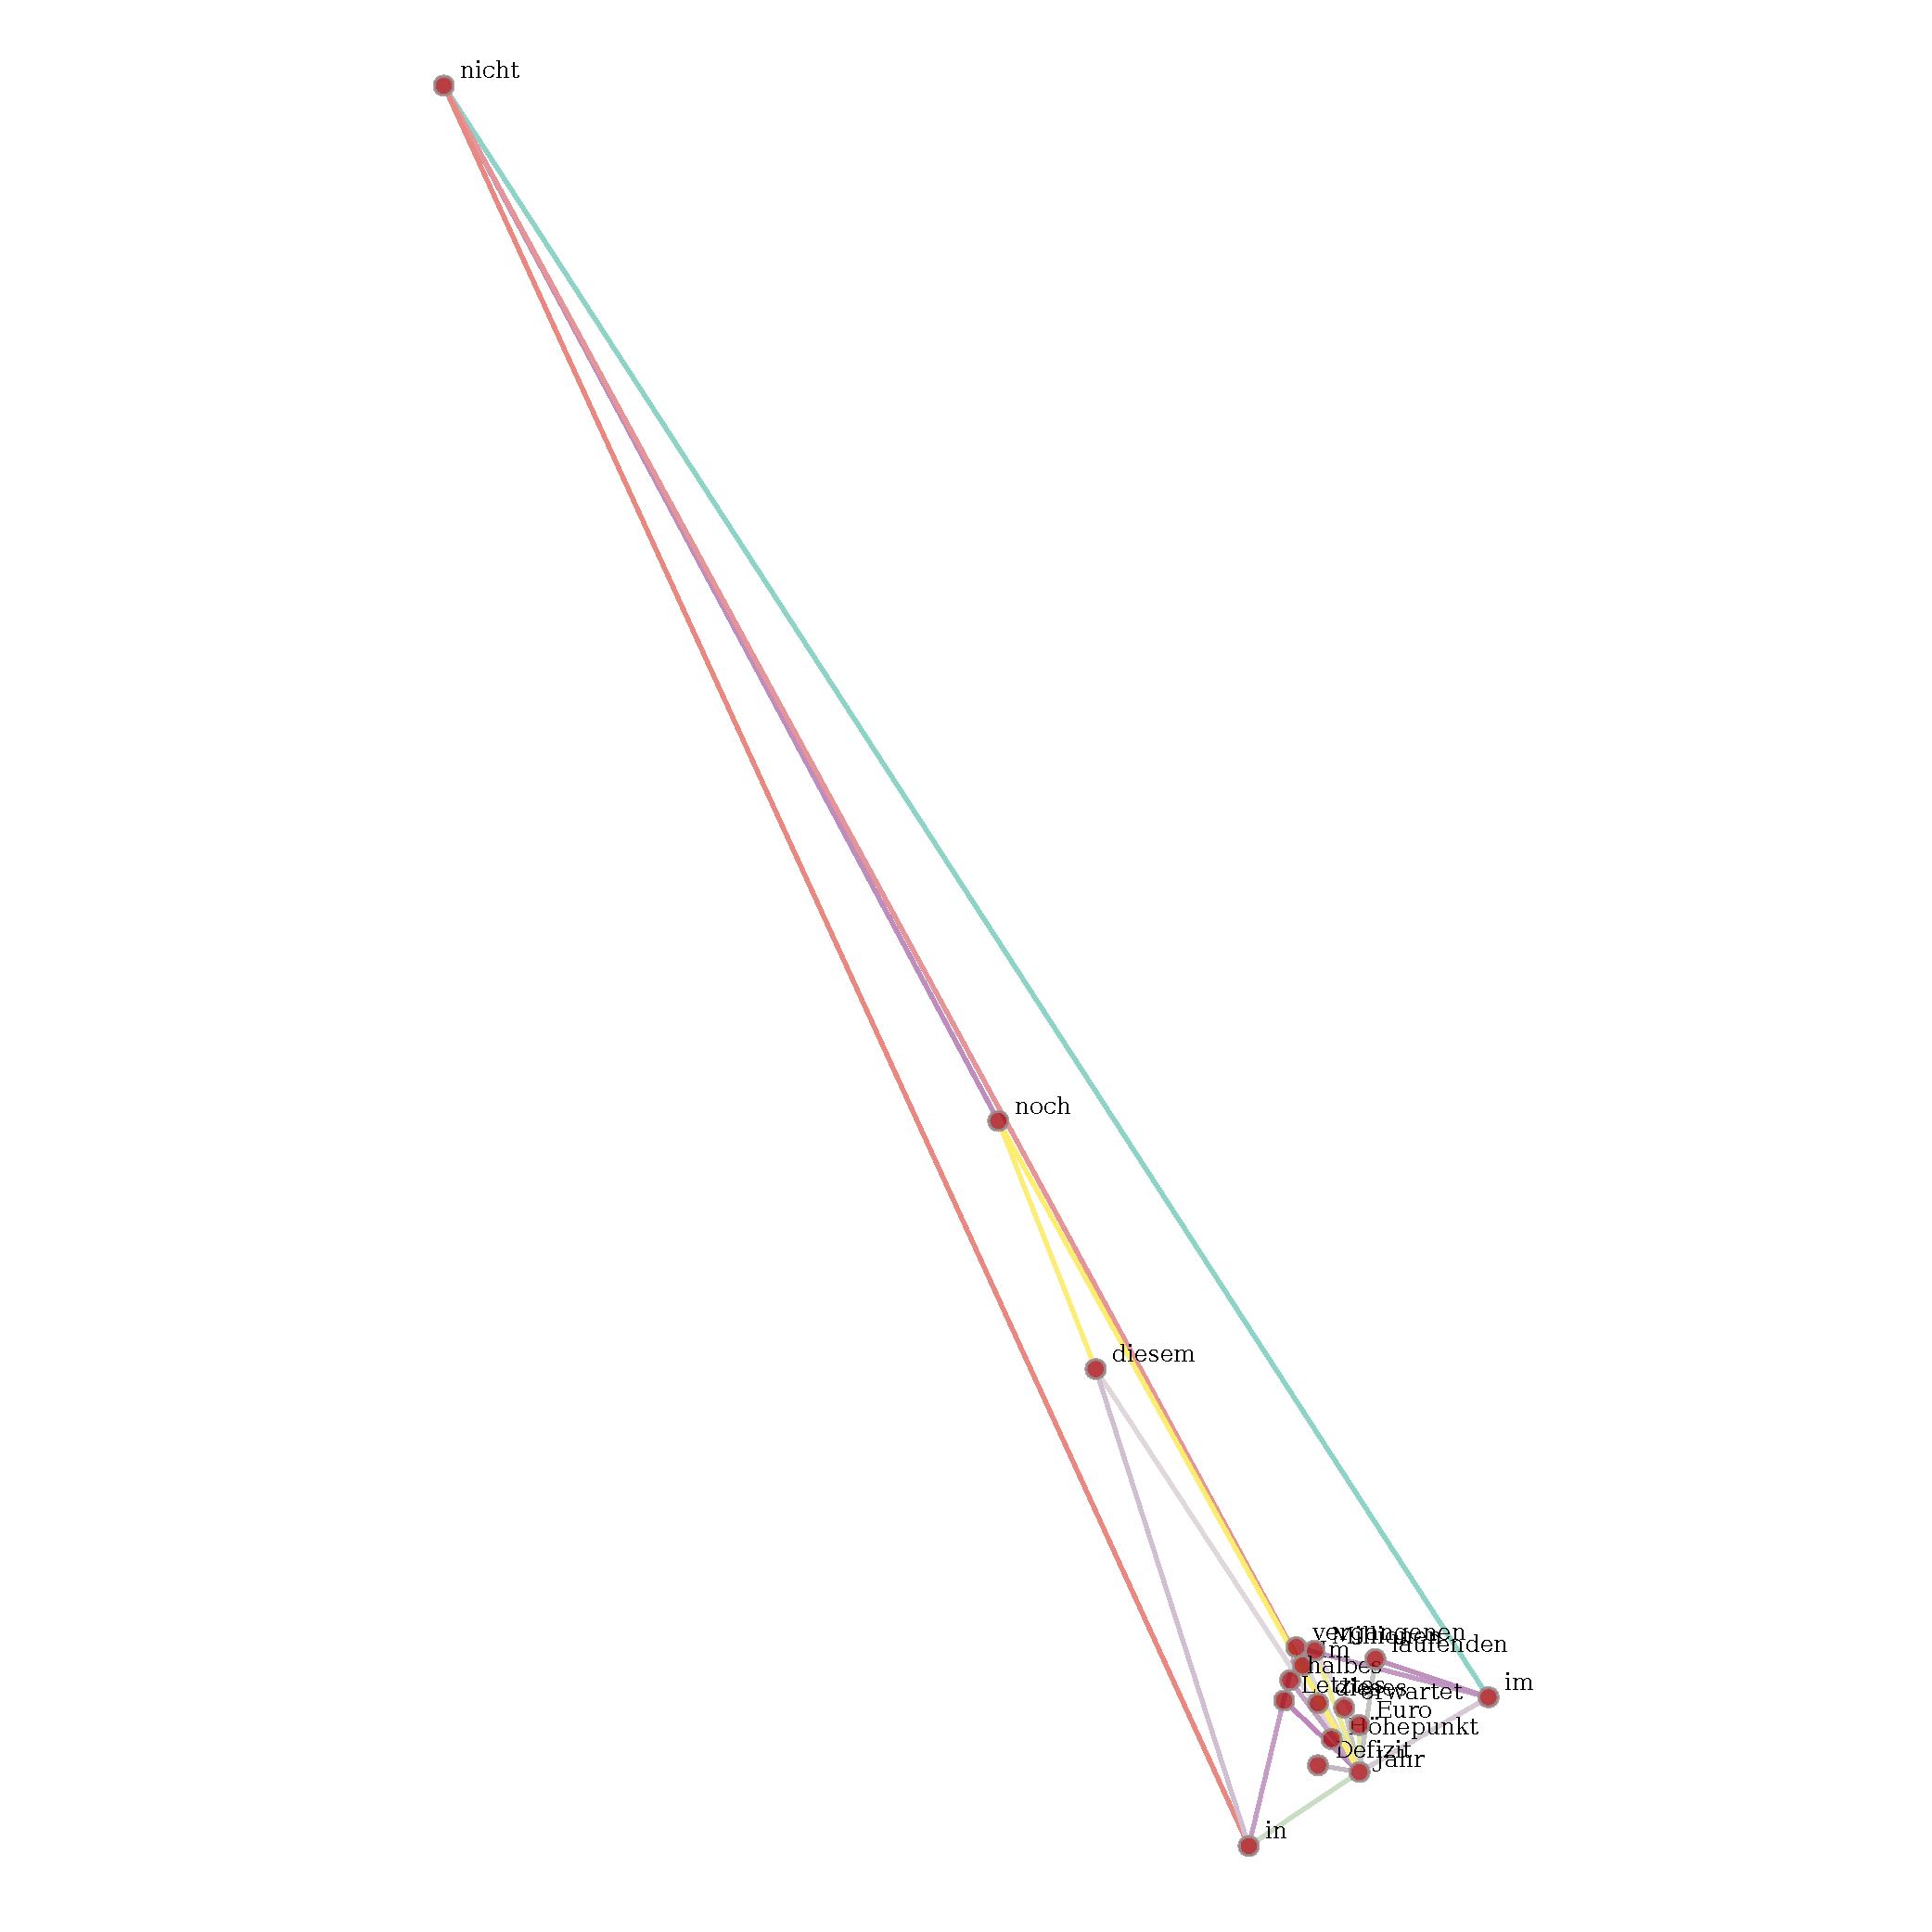
\includegraphics[scale=.4]{../../data/results/cooc_denews10k/topwords/graph_Jahr.pdf}
    \caption{Kookkurrenzgraph Jahr (Distanz 1, Schwellwert 1/12, Häufigkeit 16)}
    \label{fig:hw-jahr}
\end{figure}


\pagebreak
\subsubsection{\emph{Simple} und \emph{Standard English} Wikipedia}

\begin{figure}[hp!]
    \centering
    \begin{subfigure}[b]{0.5\textwidth}
        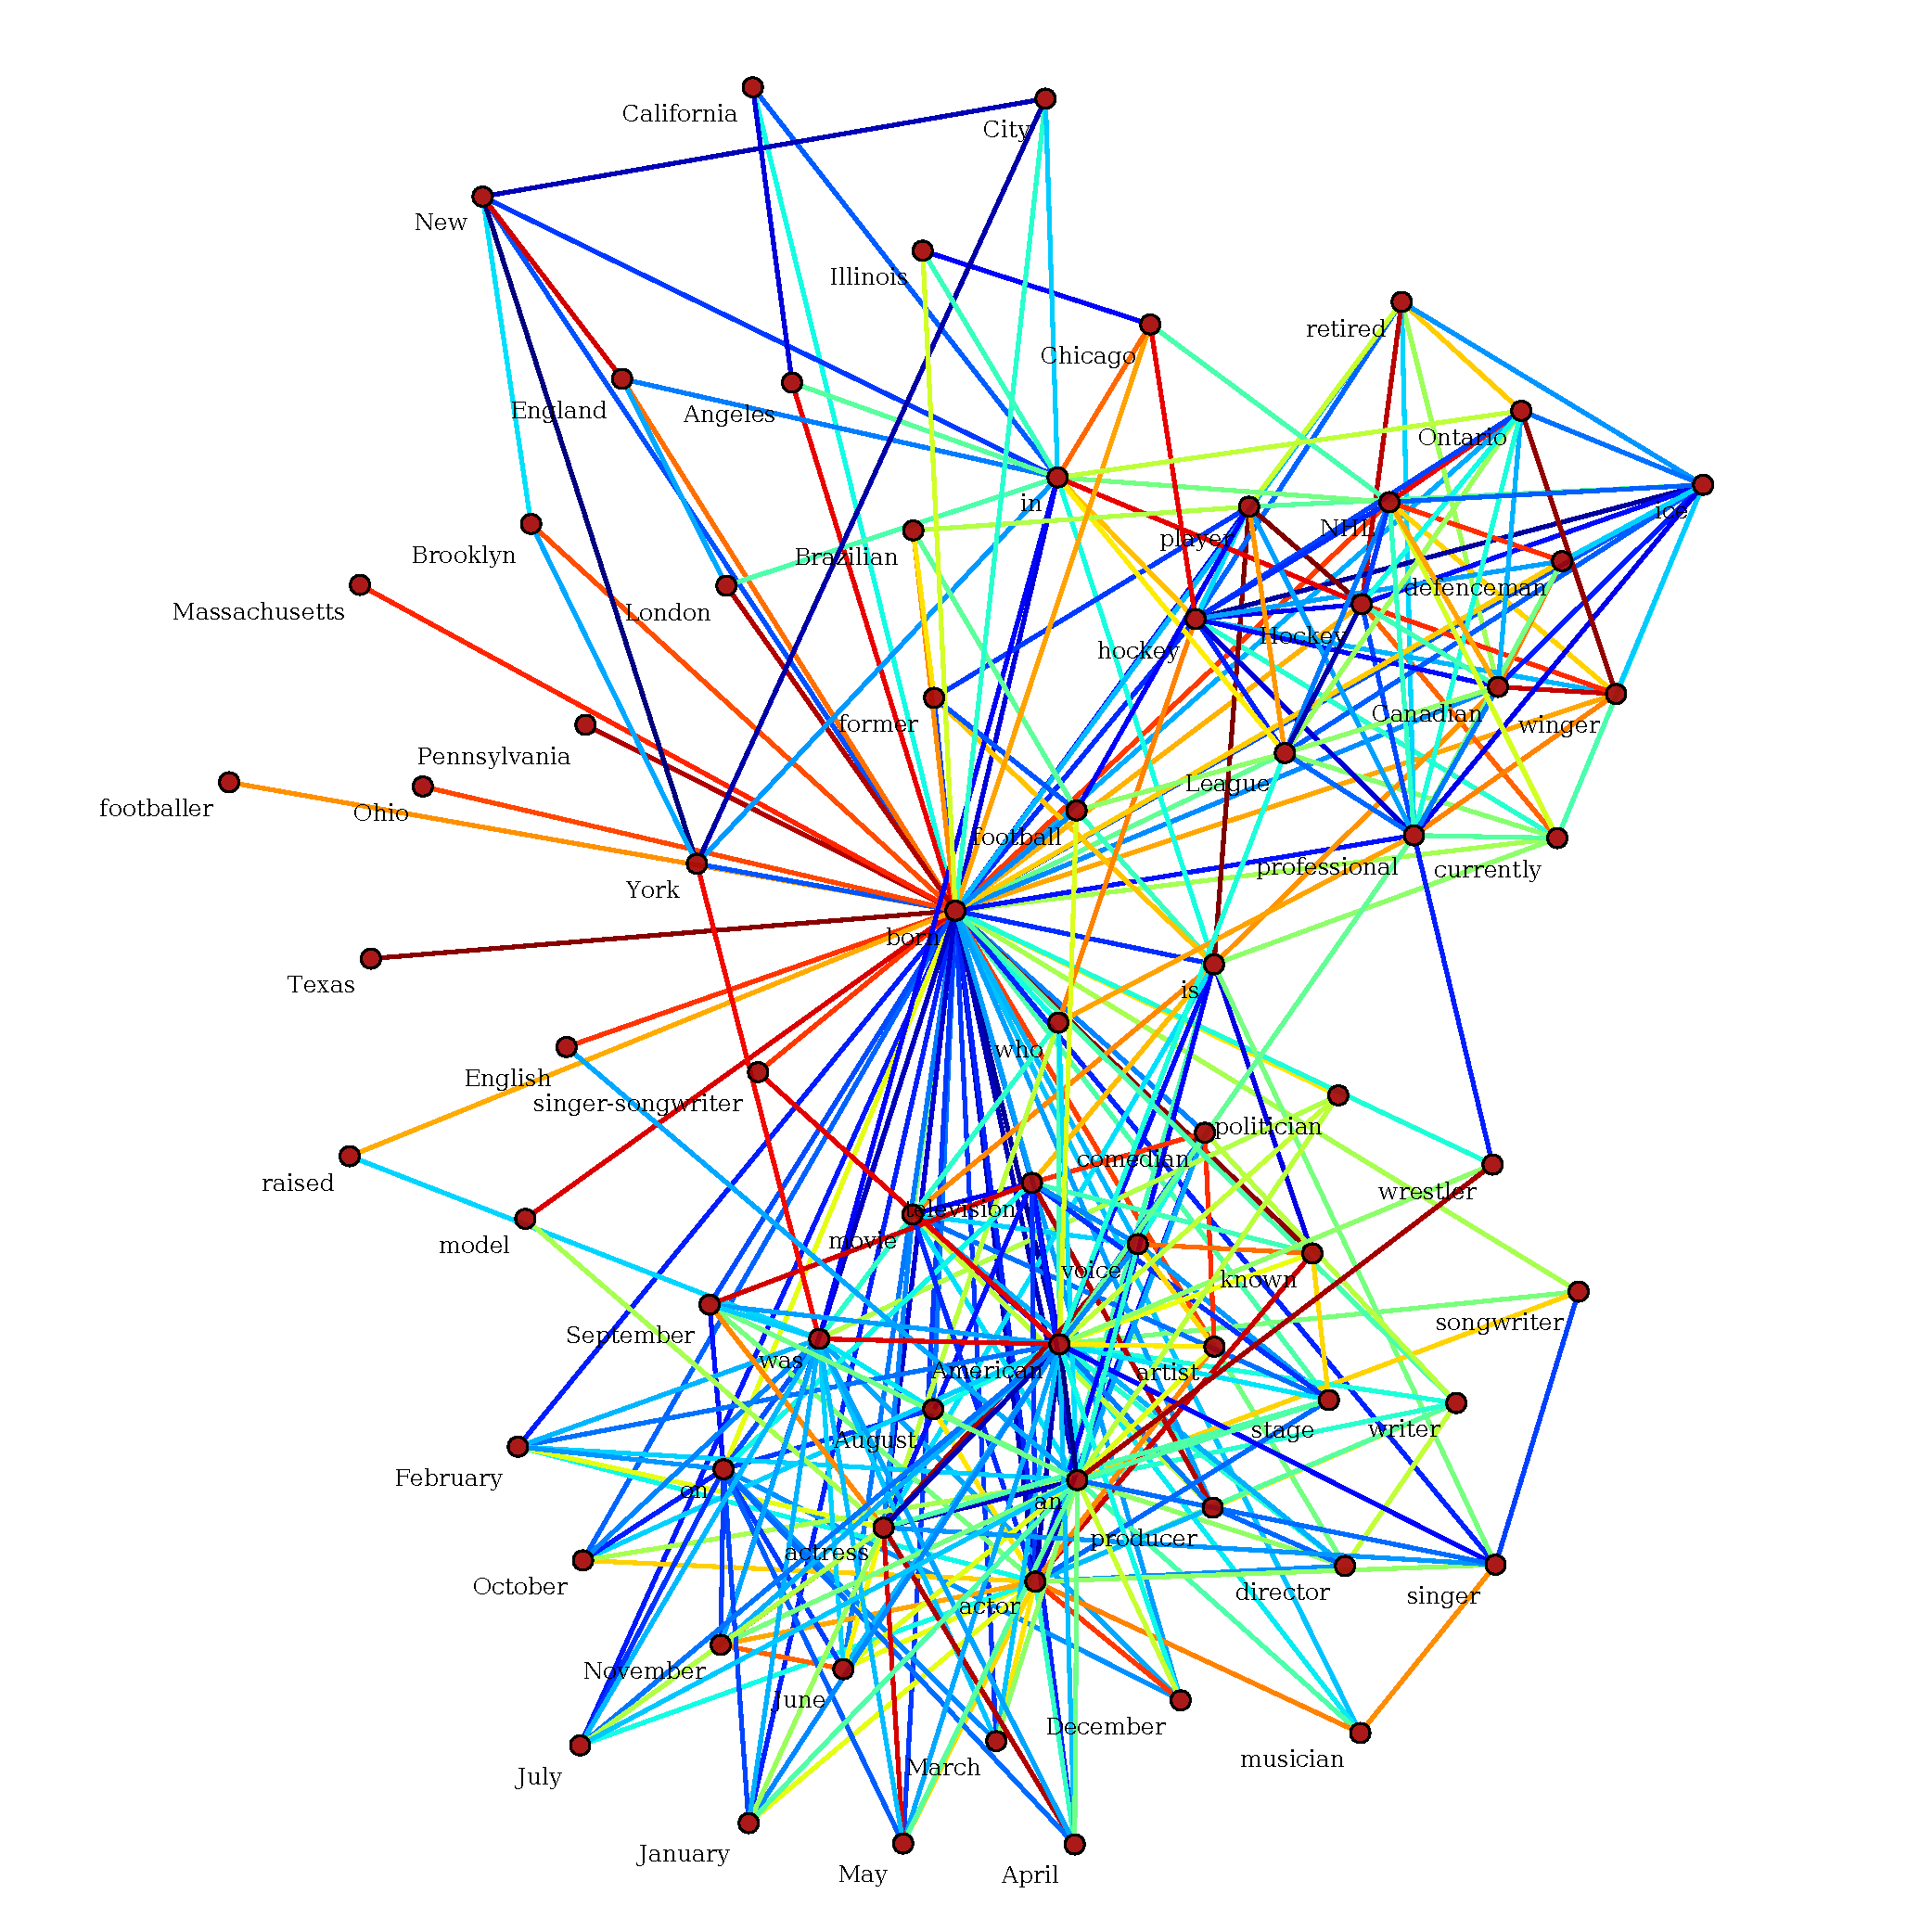
\includegraphics[scale=.25]{../../data/results/cooc_wiki_sim/topwords-t0005/graph_born.pdf}
        \caption{Simple English, Häufigkeit 71}
    \end{subfigure}
    \begin{subfigure}[b]{0.5\textwidth}
        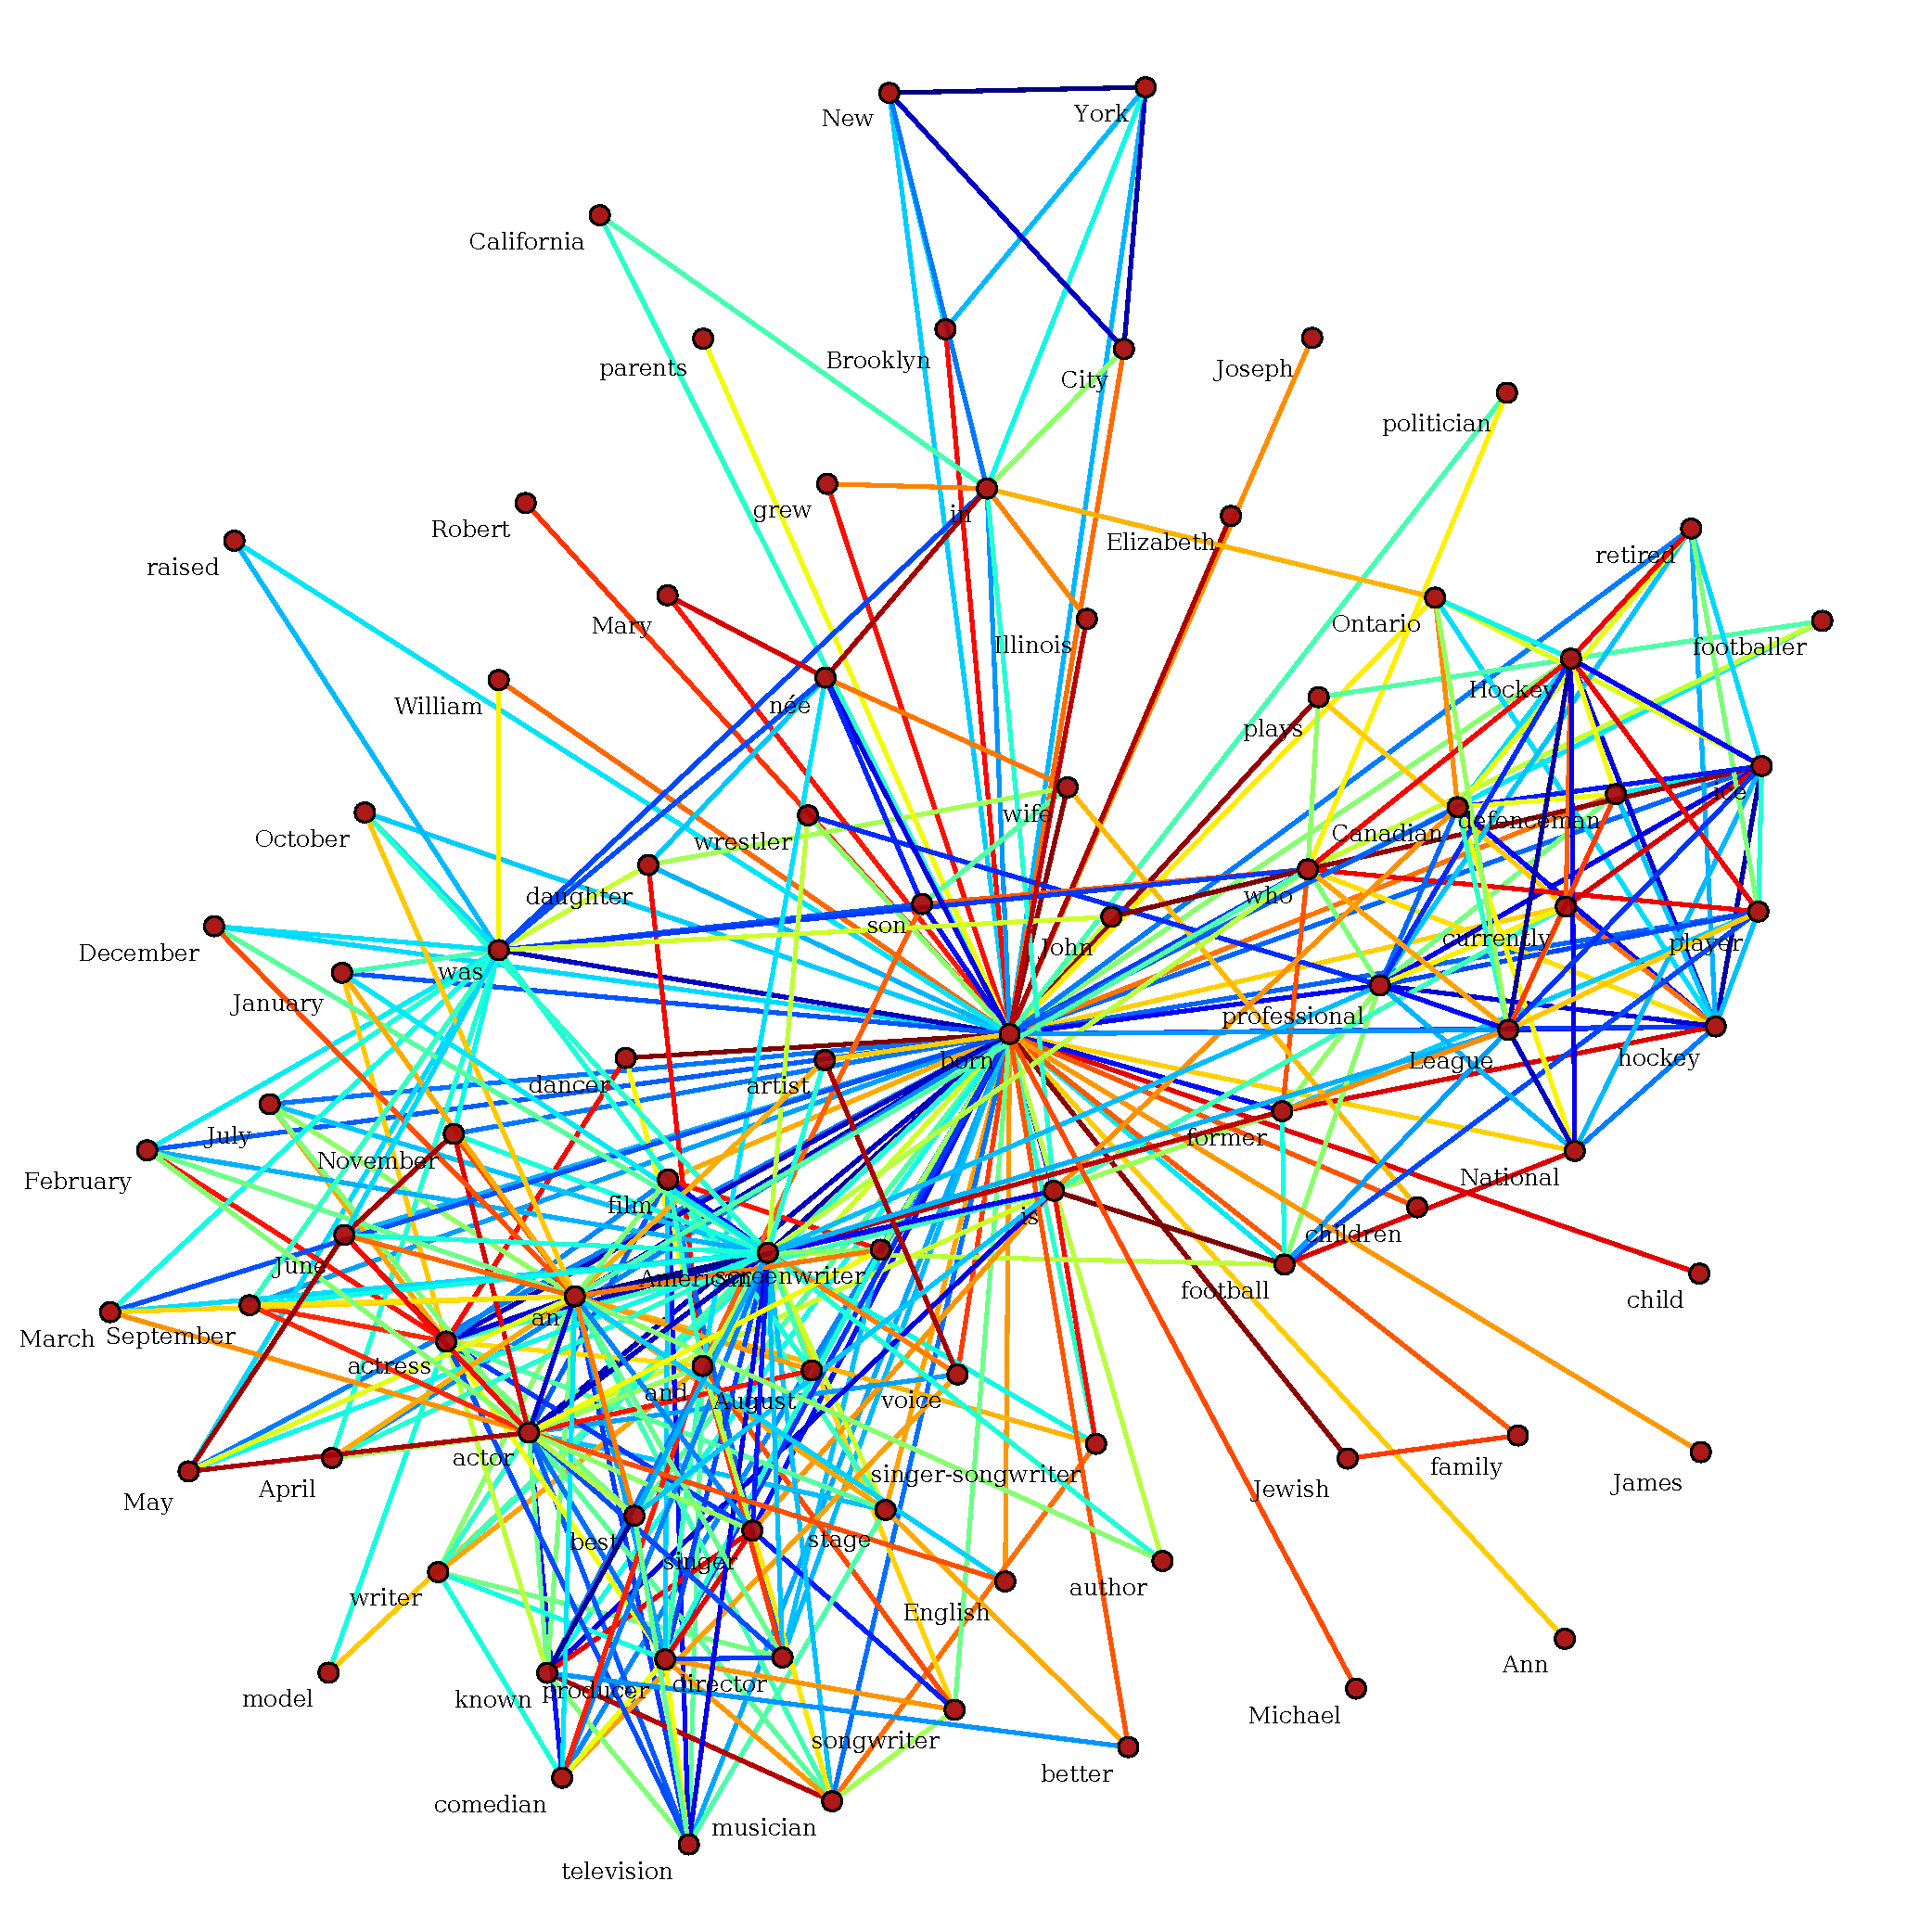
\includegraphics[scale=.25]{../../data/results/cooc_wiki_en/topwords-t0005/graph_born.pdf}
        \caption{Standard English, Häufigkeit 86}
    \end{subfigure}
    \caption{Kookkurrenzgraph born (Distanz 1, Schwellwert 0,005)}
    \label{fig:hw-born}
\end{figure}

\begin{figure}[hp!]
    \centering
    \begin{subfigure}[b]{0.5\textwidth}
        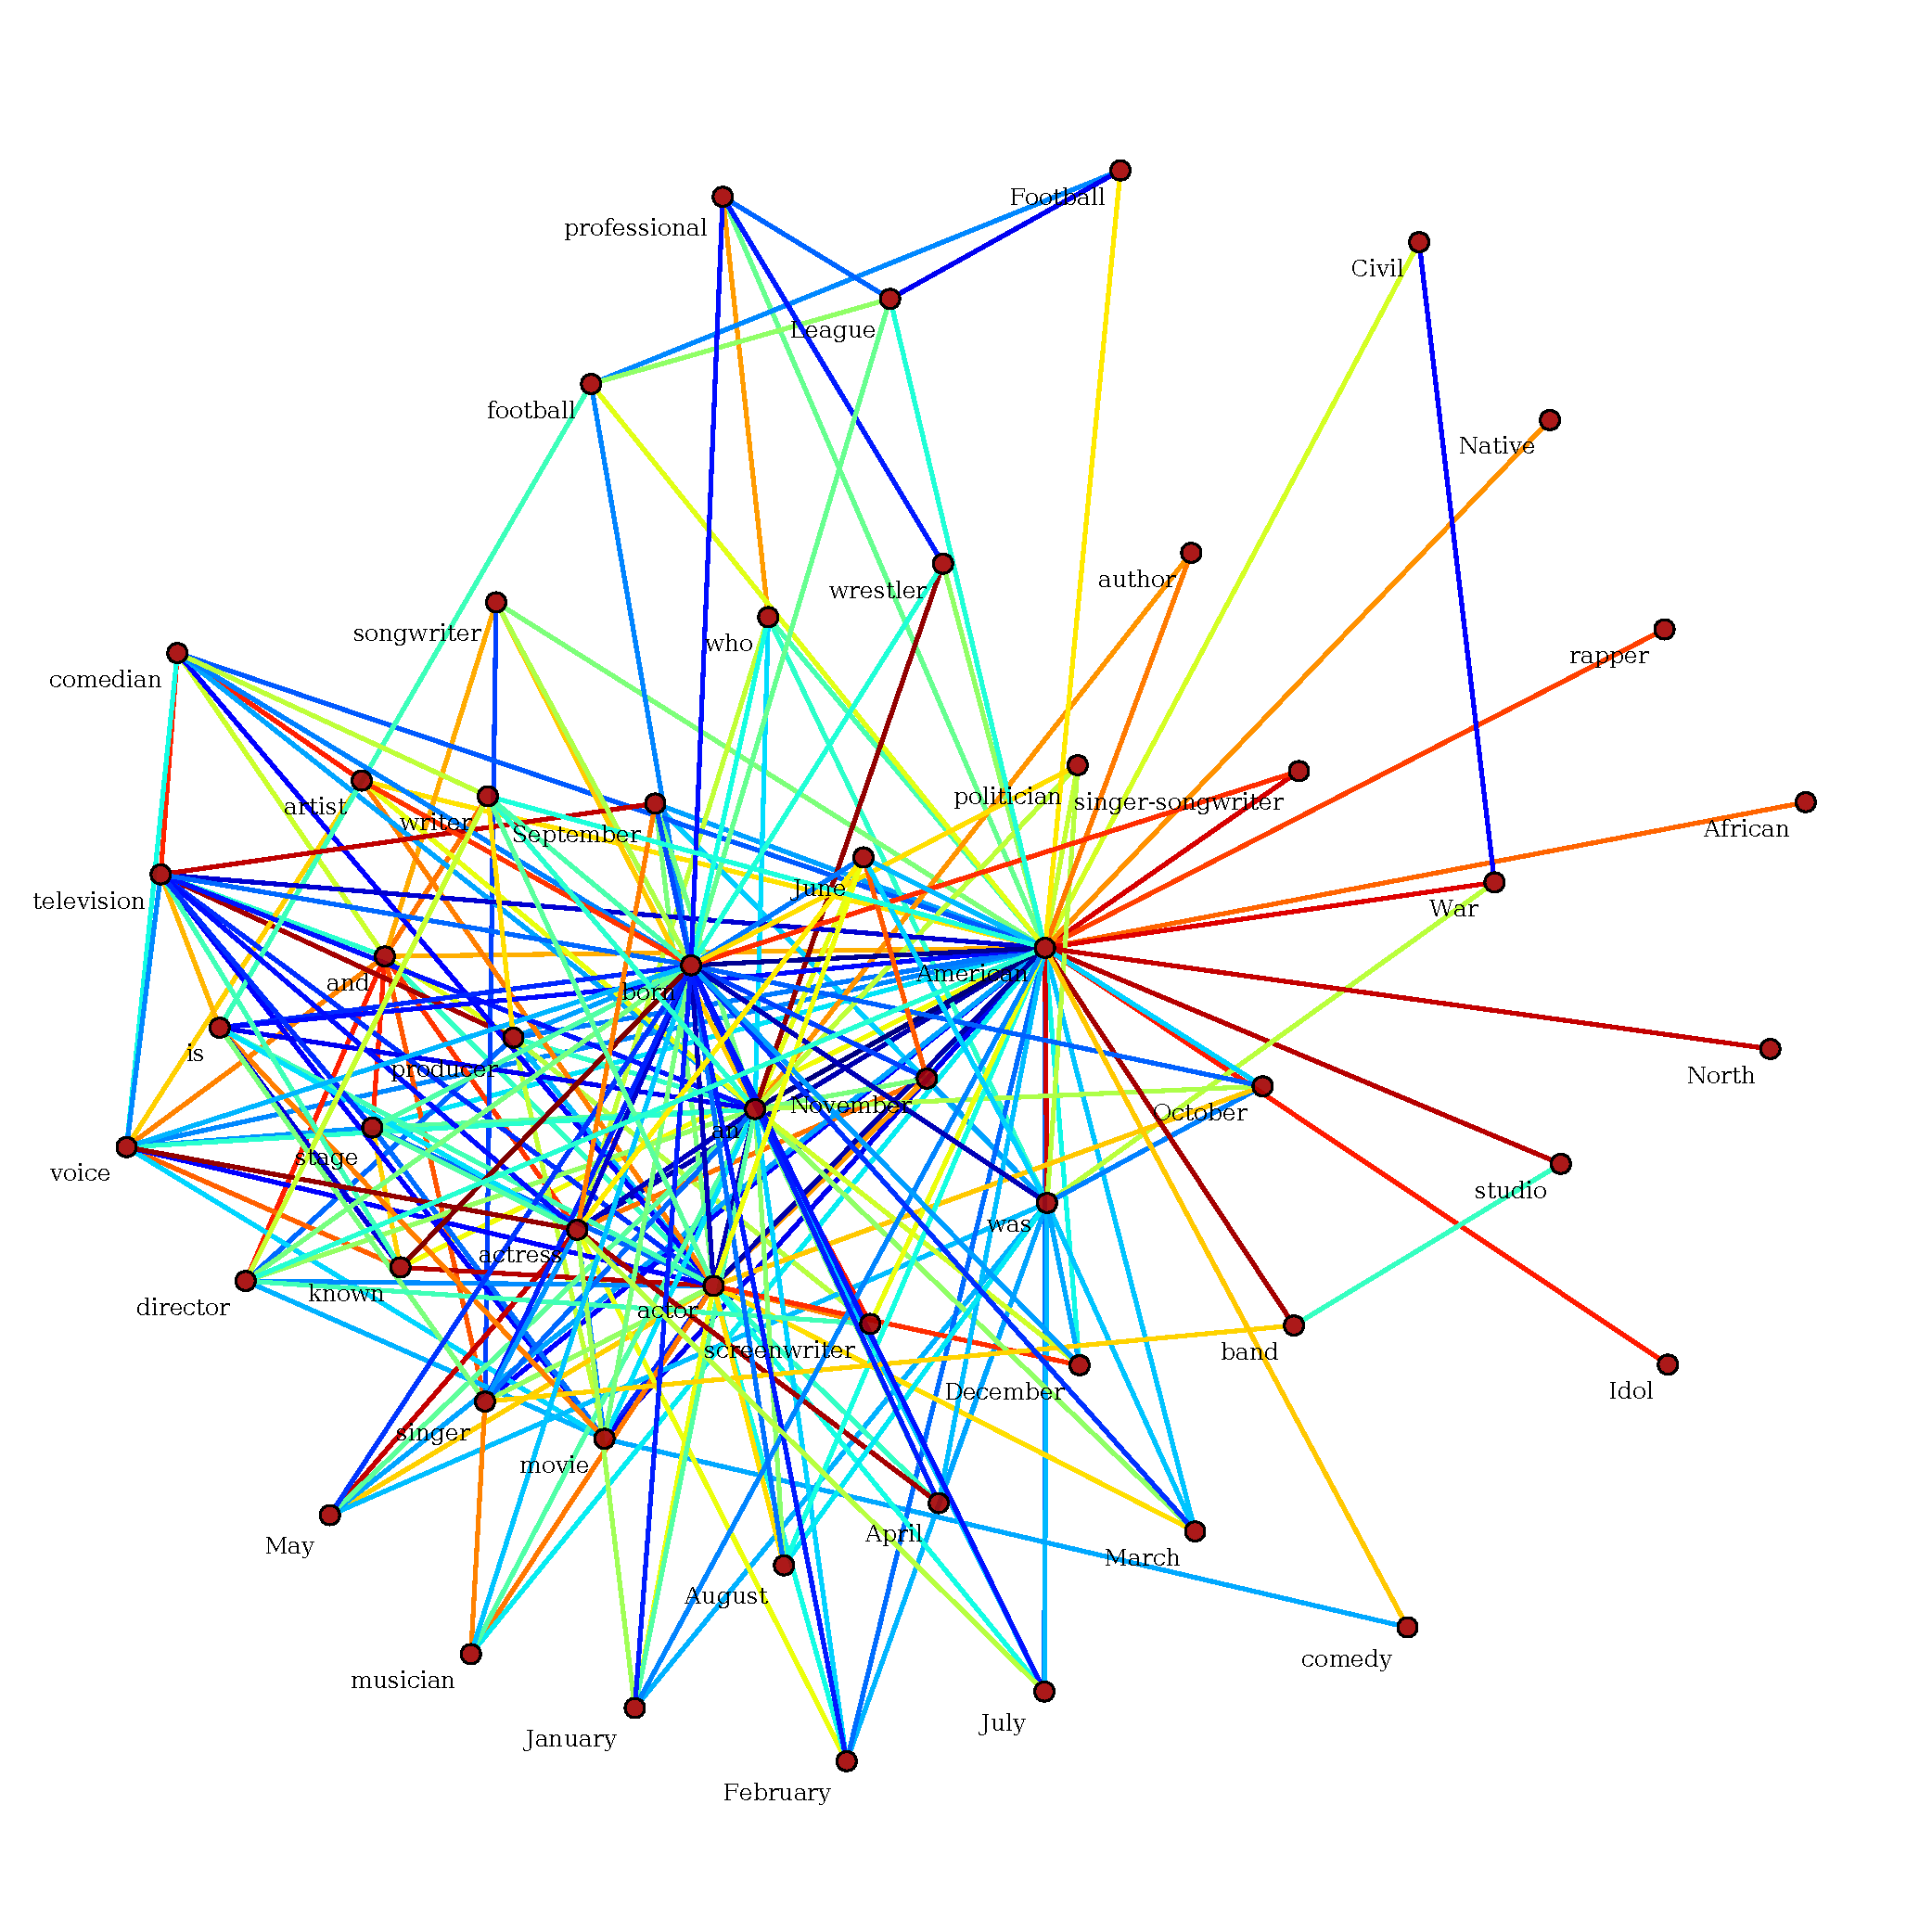
\includegraphics[scale=.25]{../../data/results/cooc_wiki_sim/topwords-t0005/graph_American.pdf}
        \caption{Simple English, Häufigkeit 52}
    \end{subfigure}
    \begin{subfigure}[b]{0.5\textwidth}
        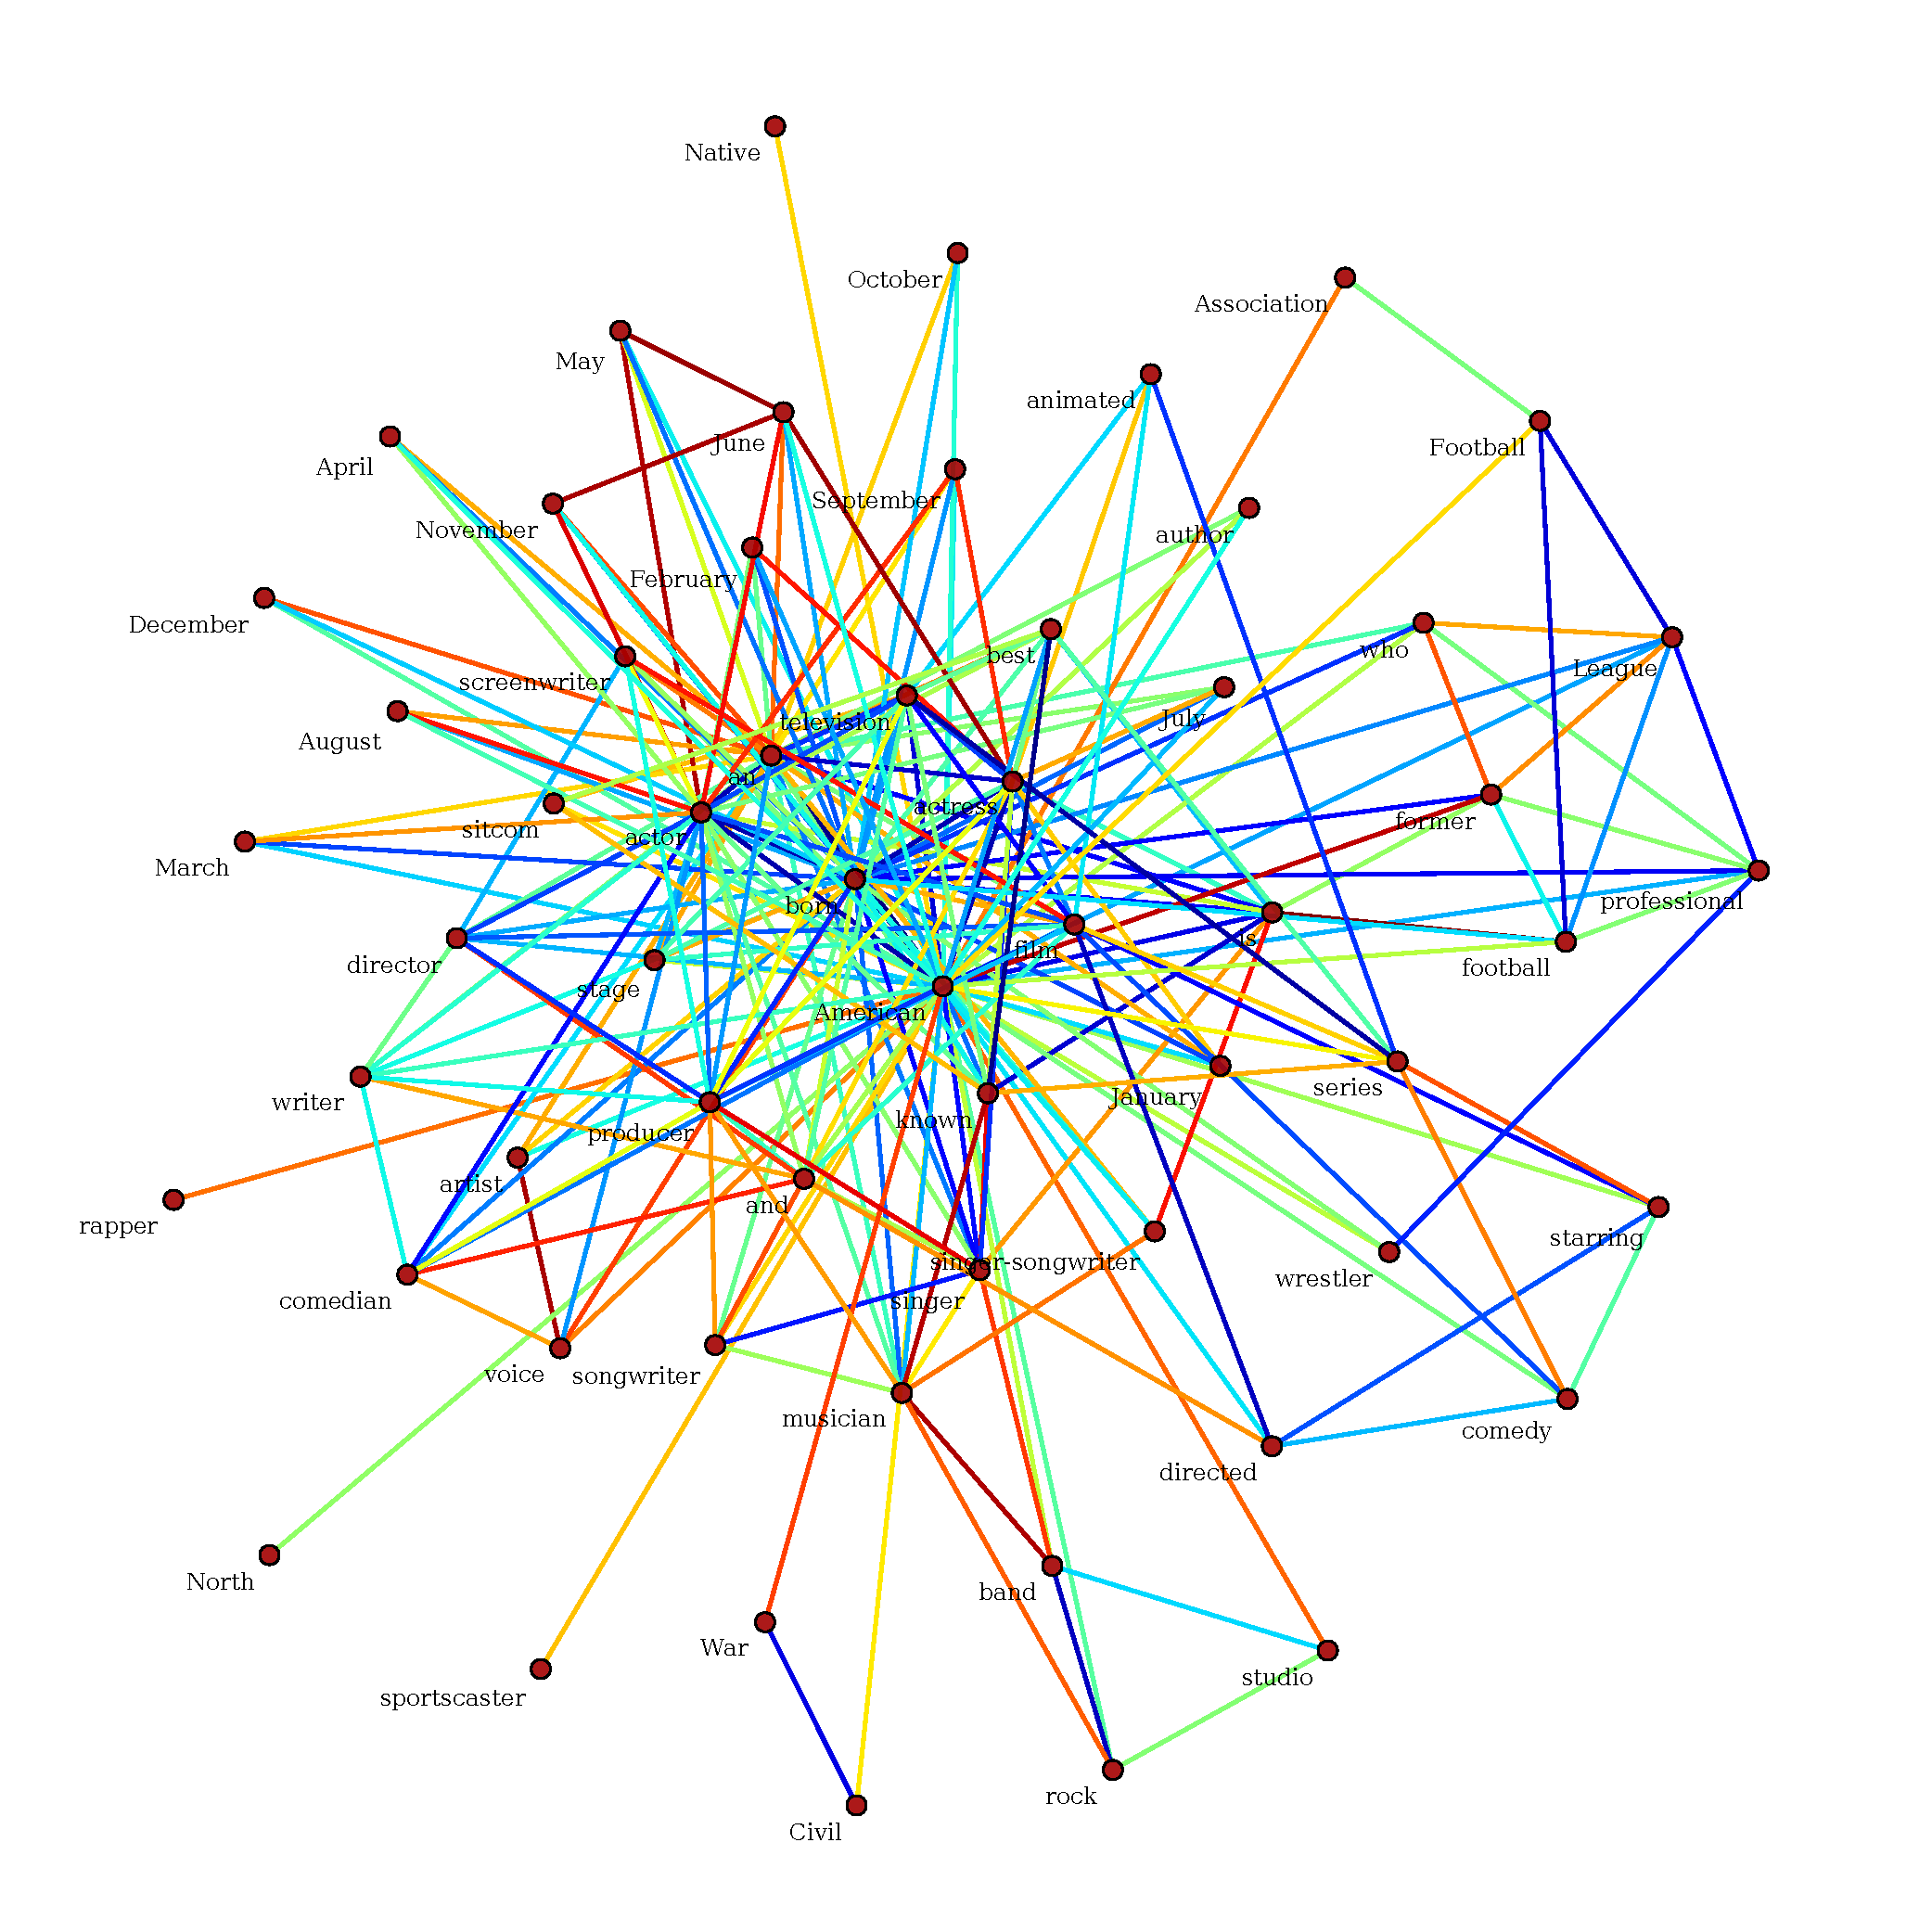
\includegraphics[scale=.25]{../../data/results/cooc_wiki_en/topwords-t0005/graph_American.pdf}
        \caption{Standard English, Häufigkeit 58}
    \end{subfigure}
    \caption{Kookkurrenzgraph American (Distanz 1, Schwellwert 0,005)}
    \label{fig:hw-american}
\end{figure}

\begin{figure}[hp!]
    \centering
    \begin{subfigure}[b]{0.5\textwidth}
        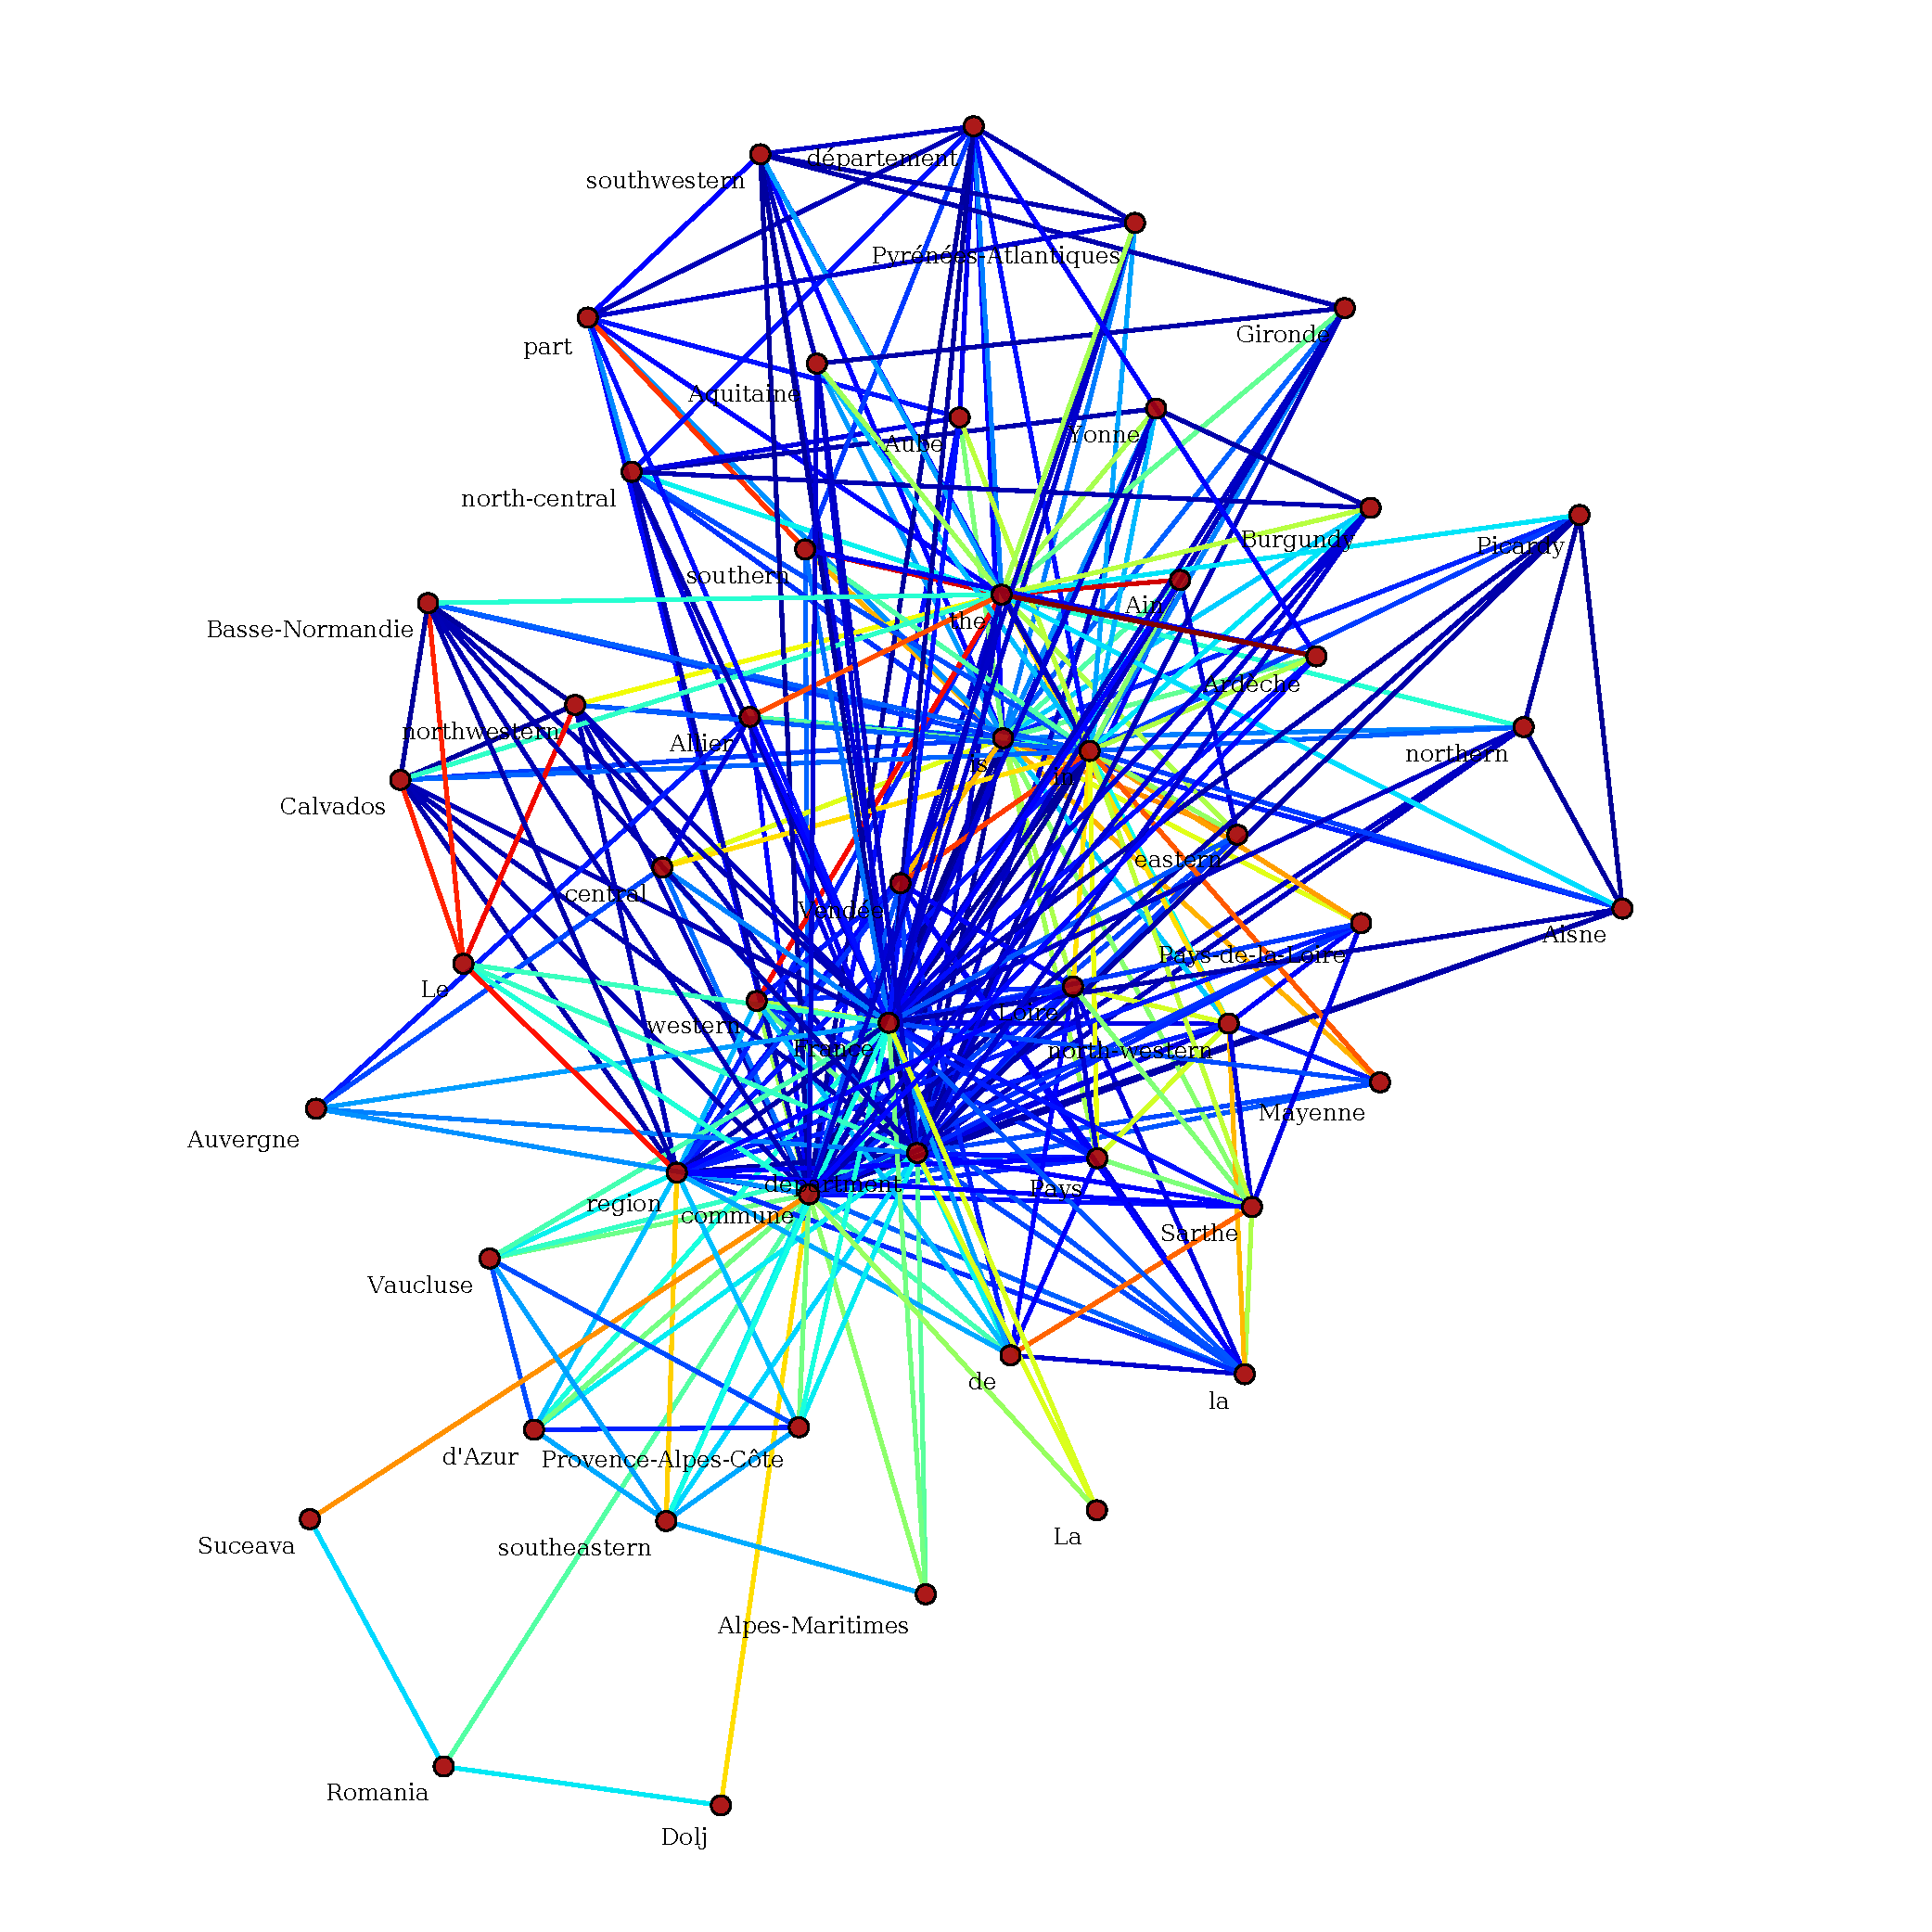
\includegraphics[scale=.25]{../../data/results/cooc_wiki_sim/topwords-t0005/graph_commune.pdf}
        \caption{Simple English, Häufigkeit 49}
    \end{subfigure}
    \begin{subfigure}[b]{0.5\textwidth}
        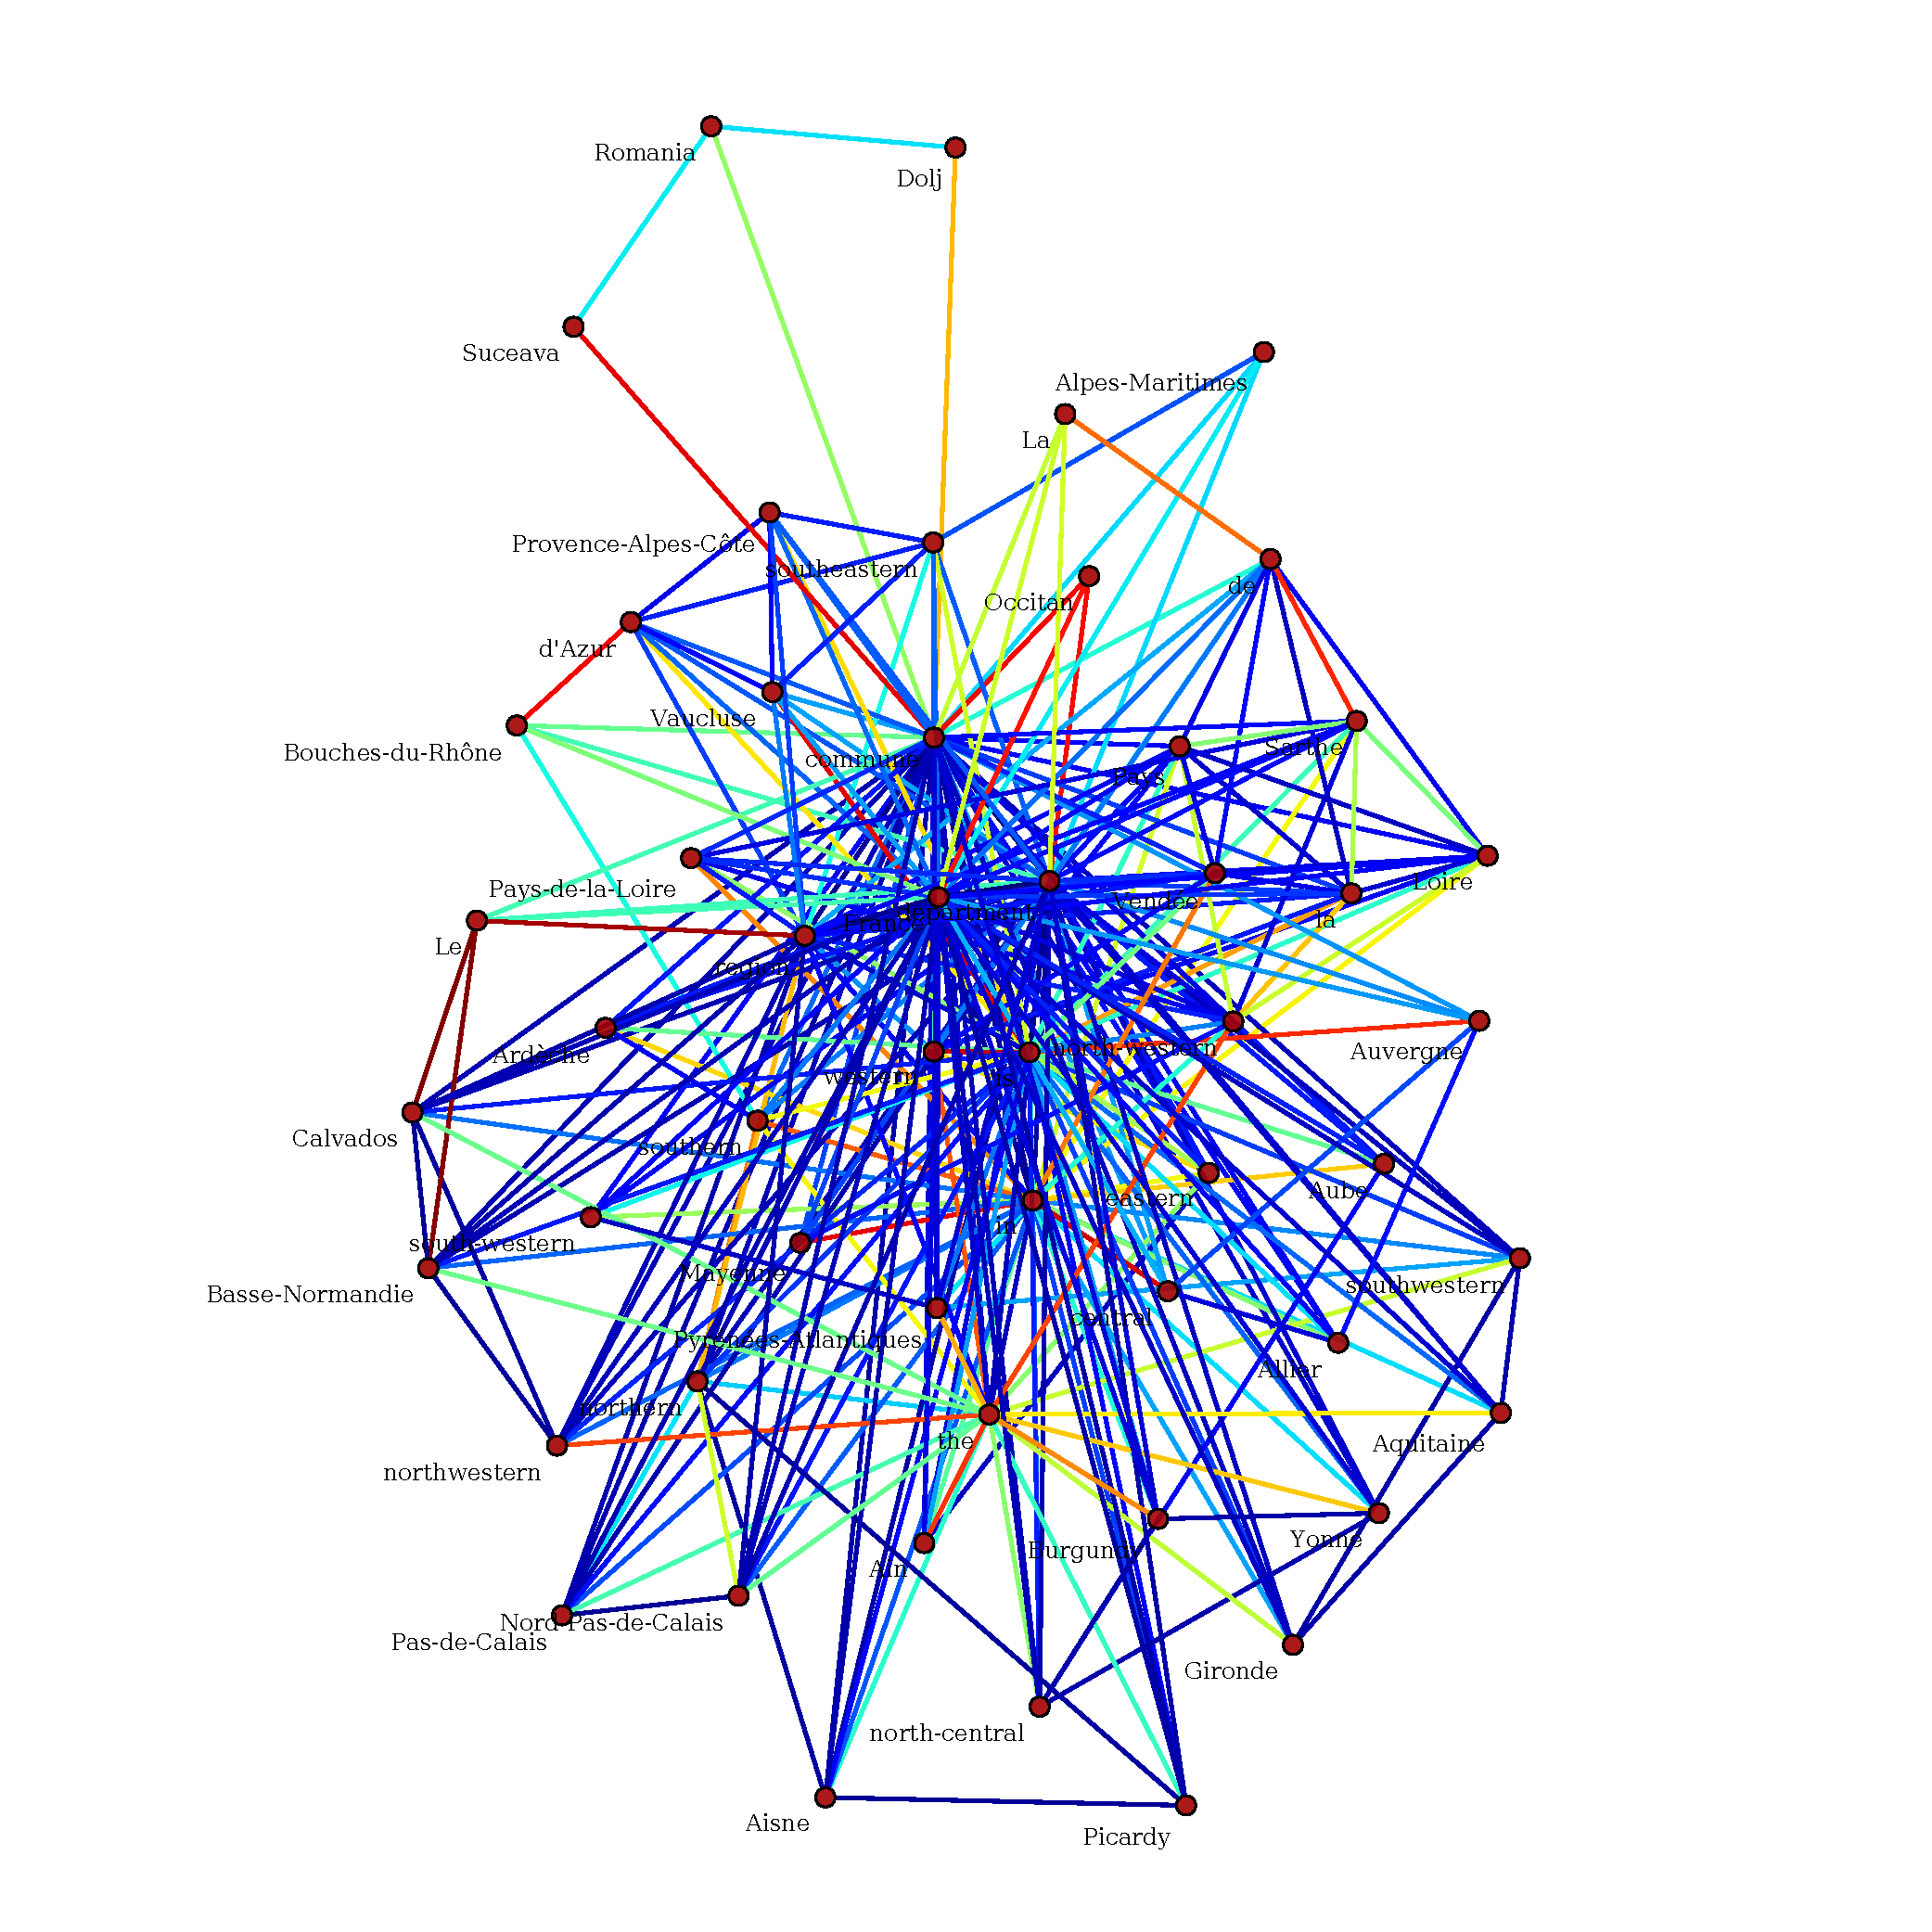
\includegraphics[scale=.25]{../../data/results/cooc_wiki_en/topwords-t0005/graph_commune.pdf}
        \caption{Standard English, Häufigkeit 52}
    \end{subfigure}
    \caption{Kookkurrenzgraph commune (Distanz 1, Schwellwert 0,005)}
    \label{fig:hw-commune}
\end{figure}

\begin{figure}[hp!]
    \centering
    \begin{subfigure}[b]{0.5\textwidth}
        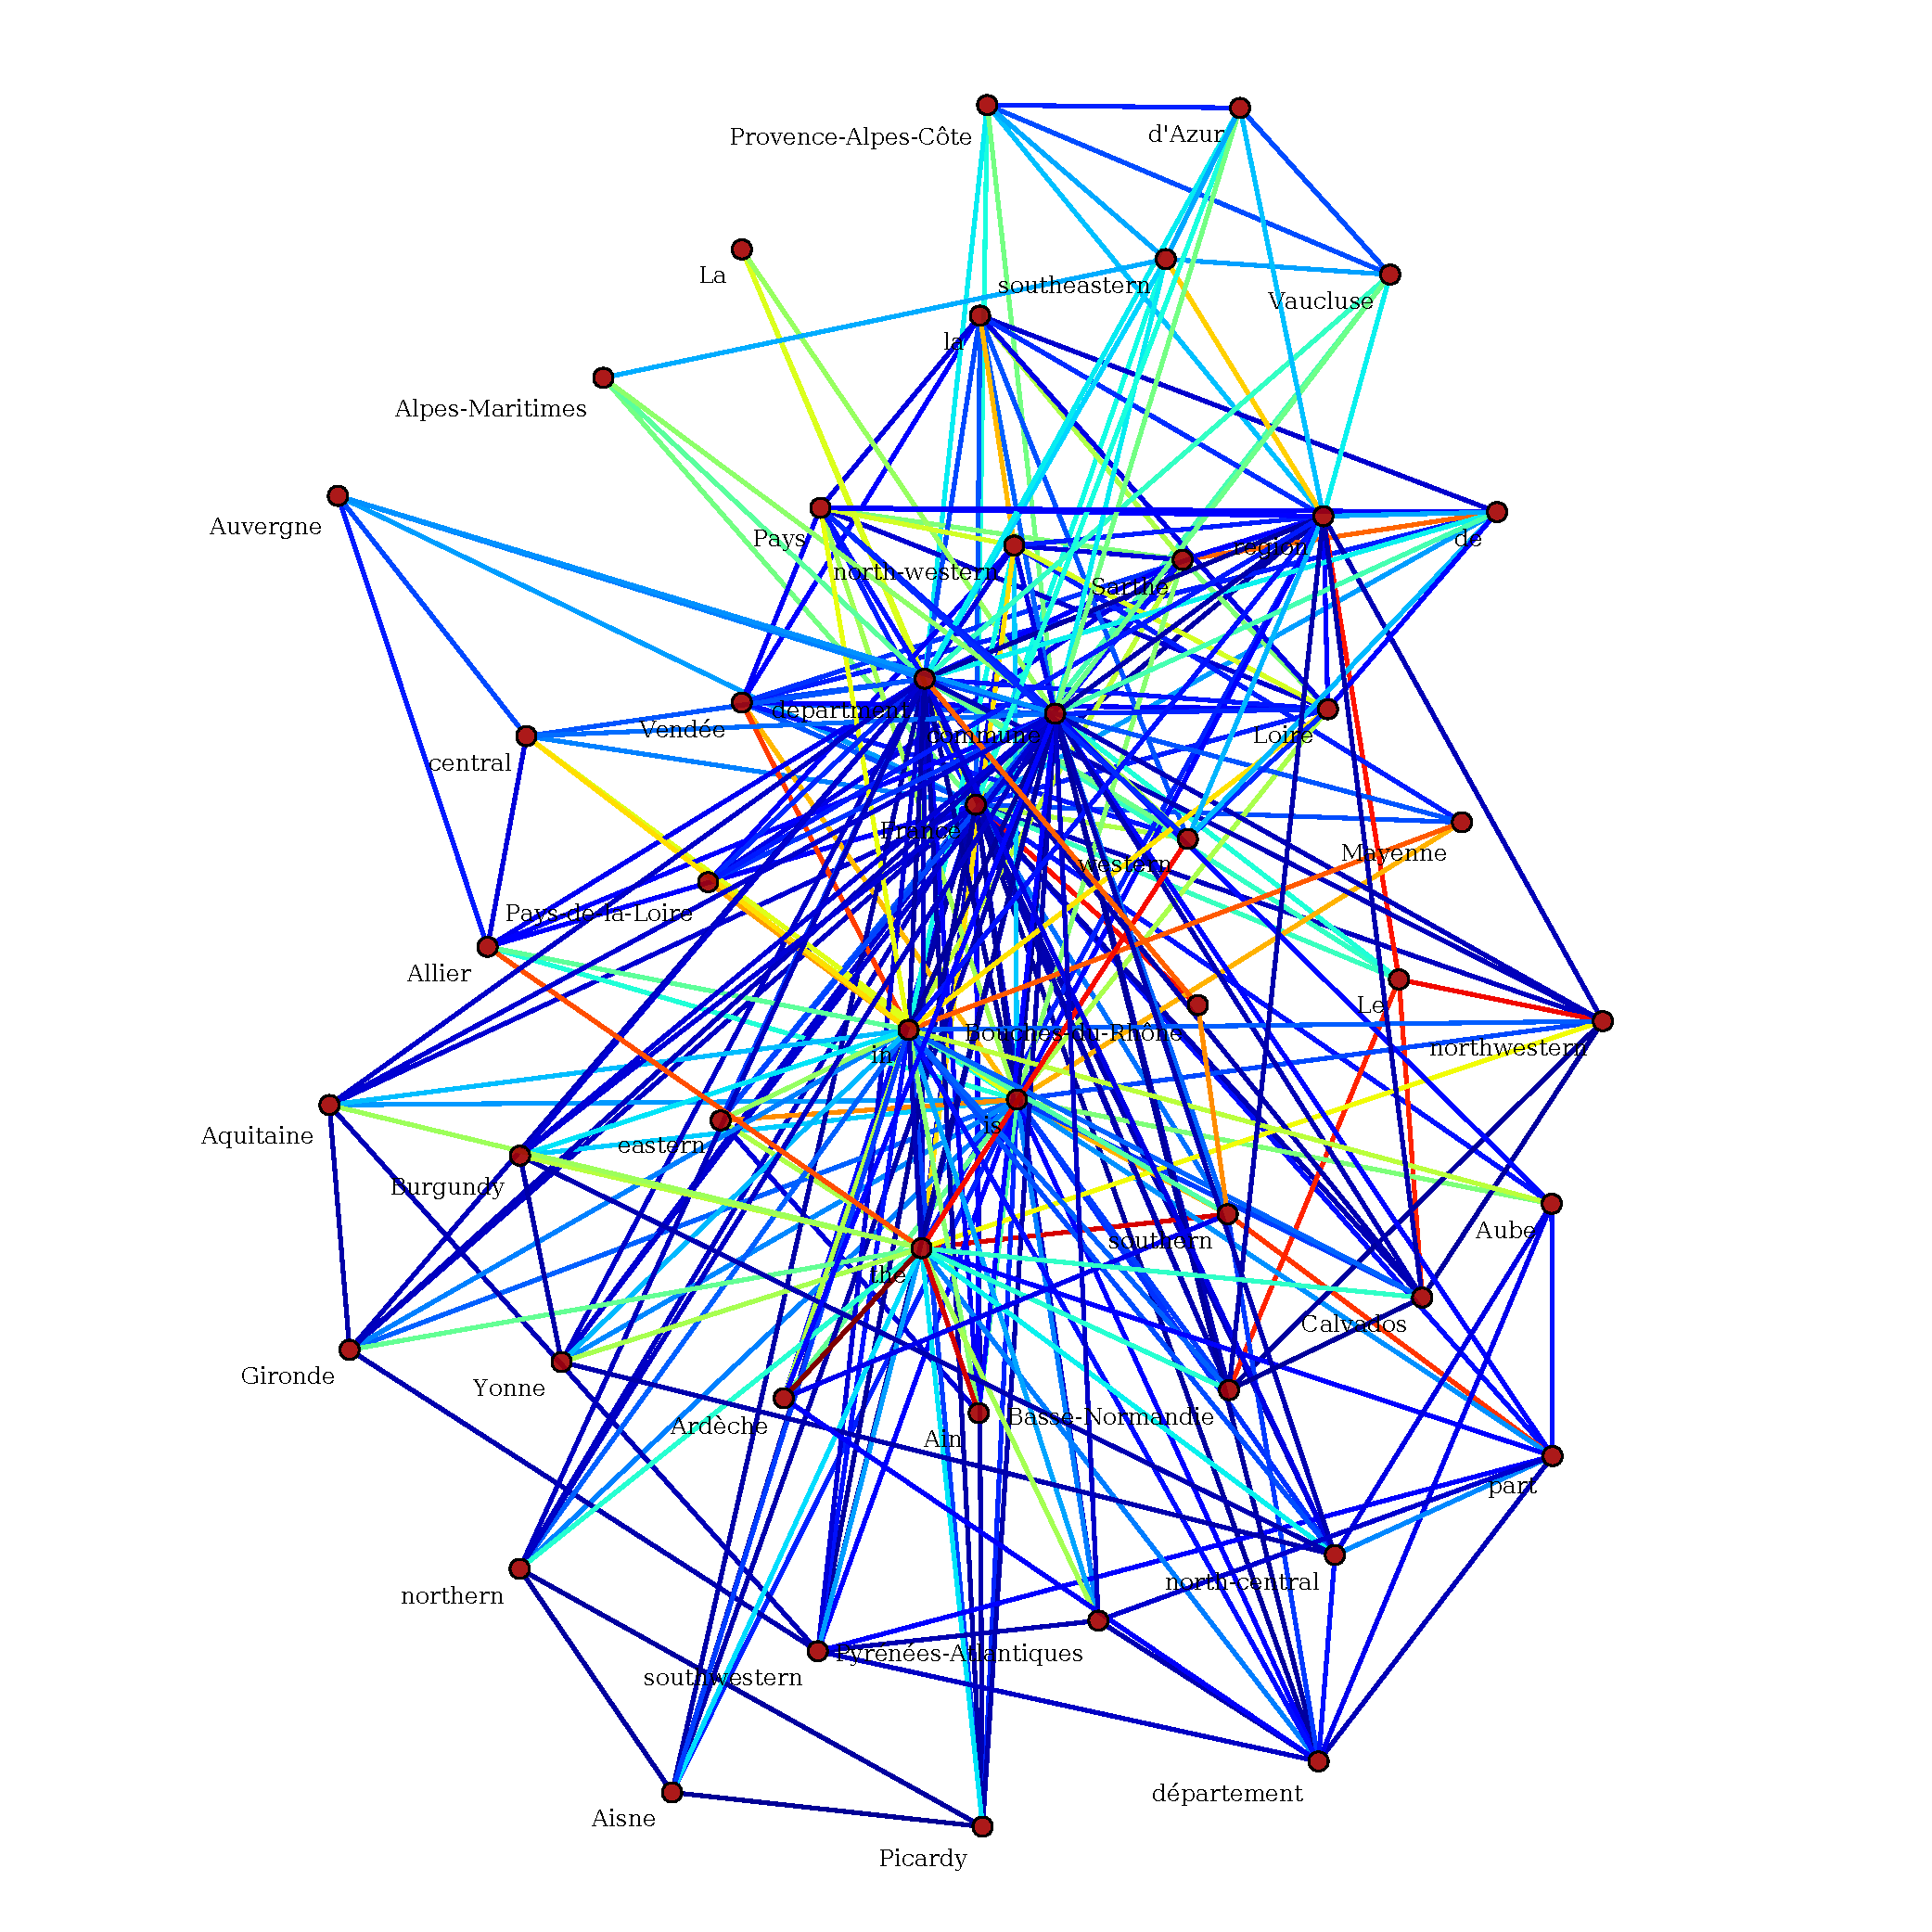
\includegraphics[scale=.25]{../../data/results/cooc_wiki_sim/topwords-t0005/graph_France.pdf}
        \caption{Simple English, Häufigkeit 47}
    \end{subfigure}
    \begin{subfigure}[b]{0.5\textwidth}
        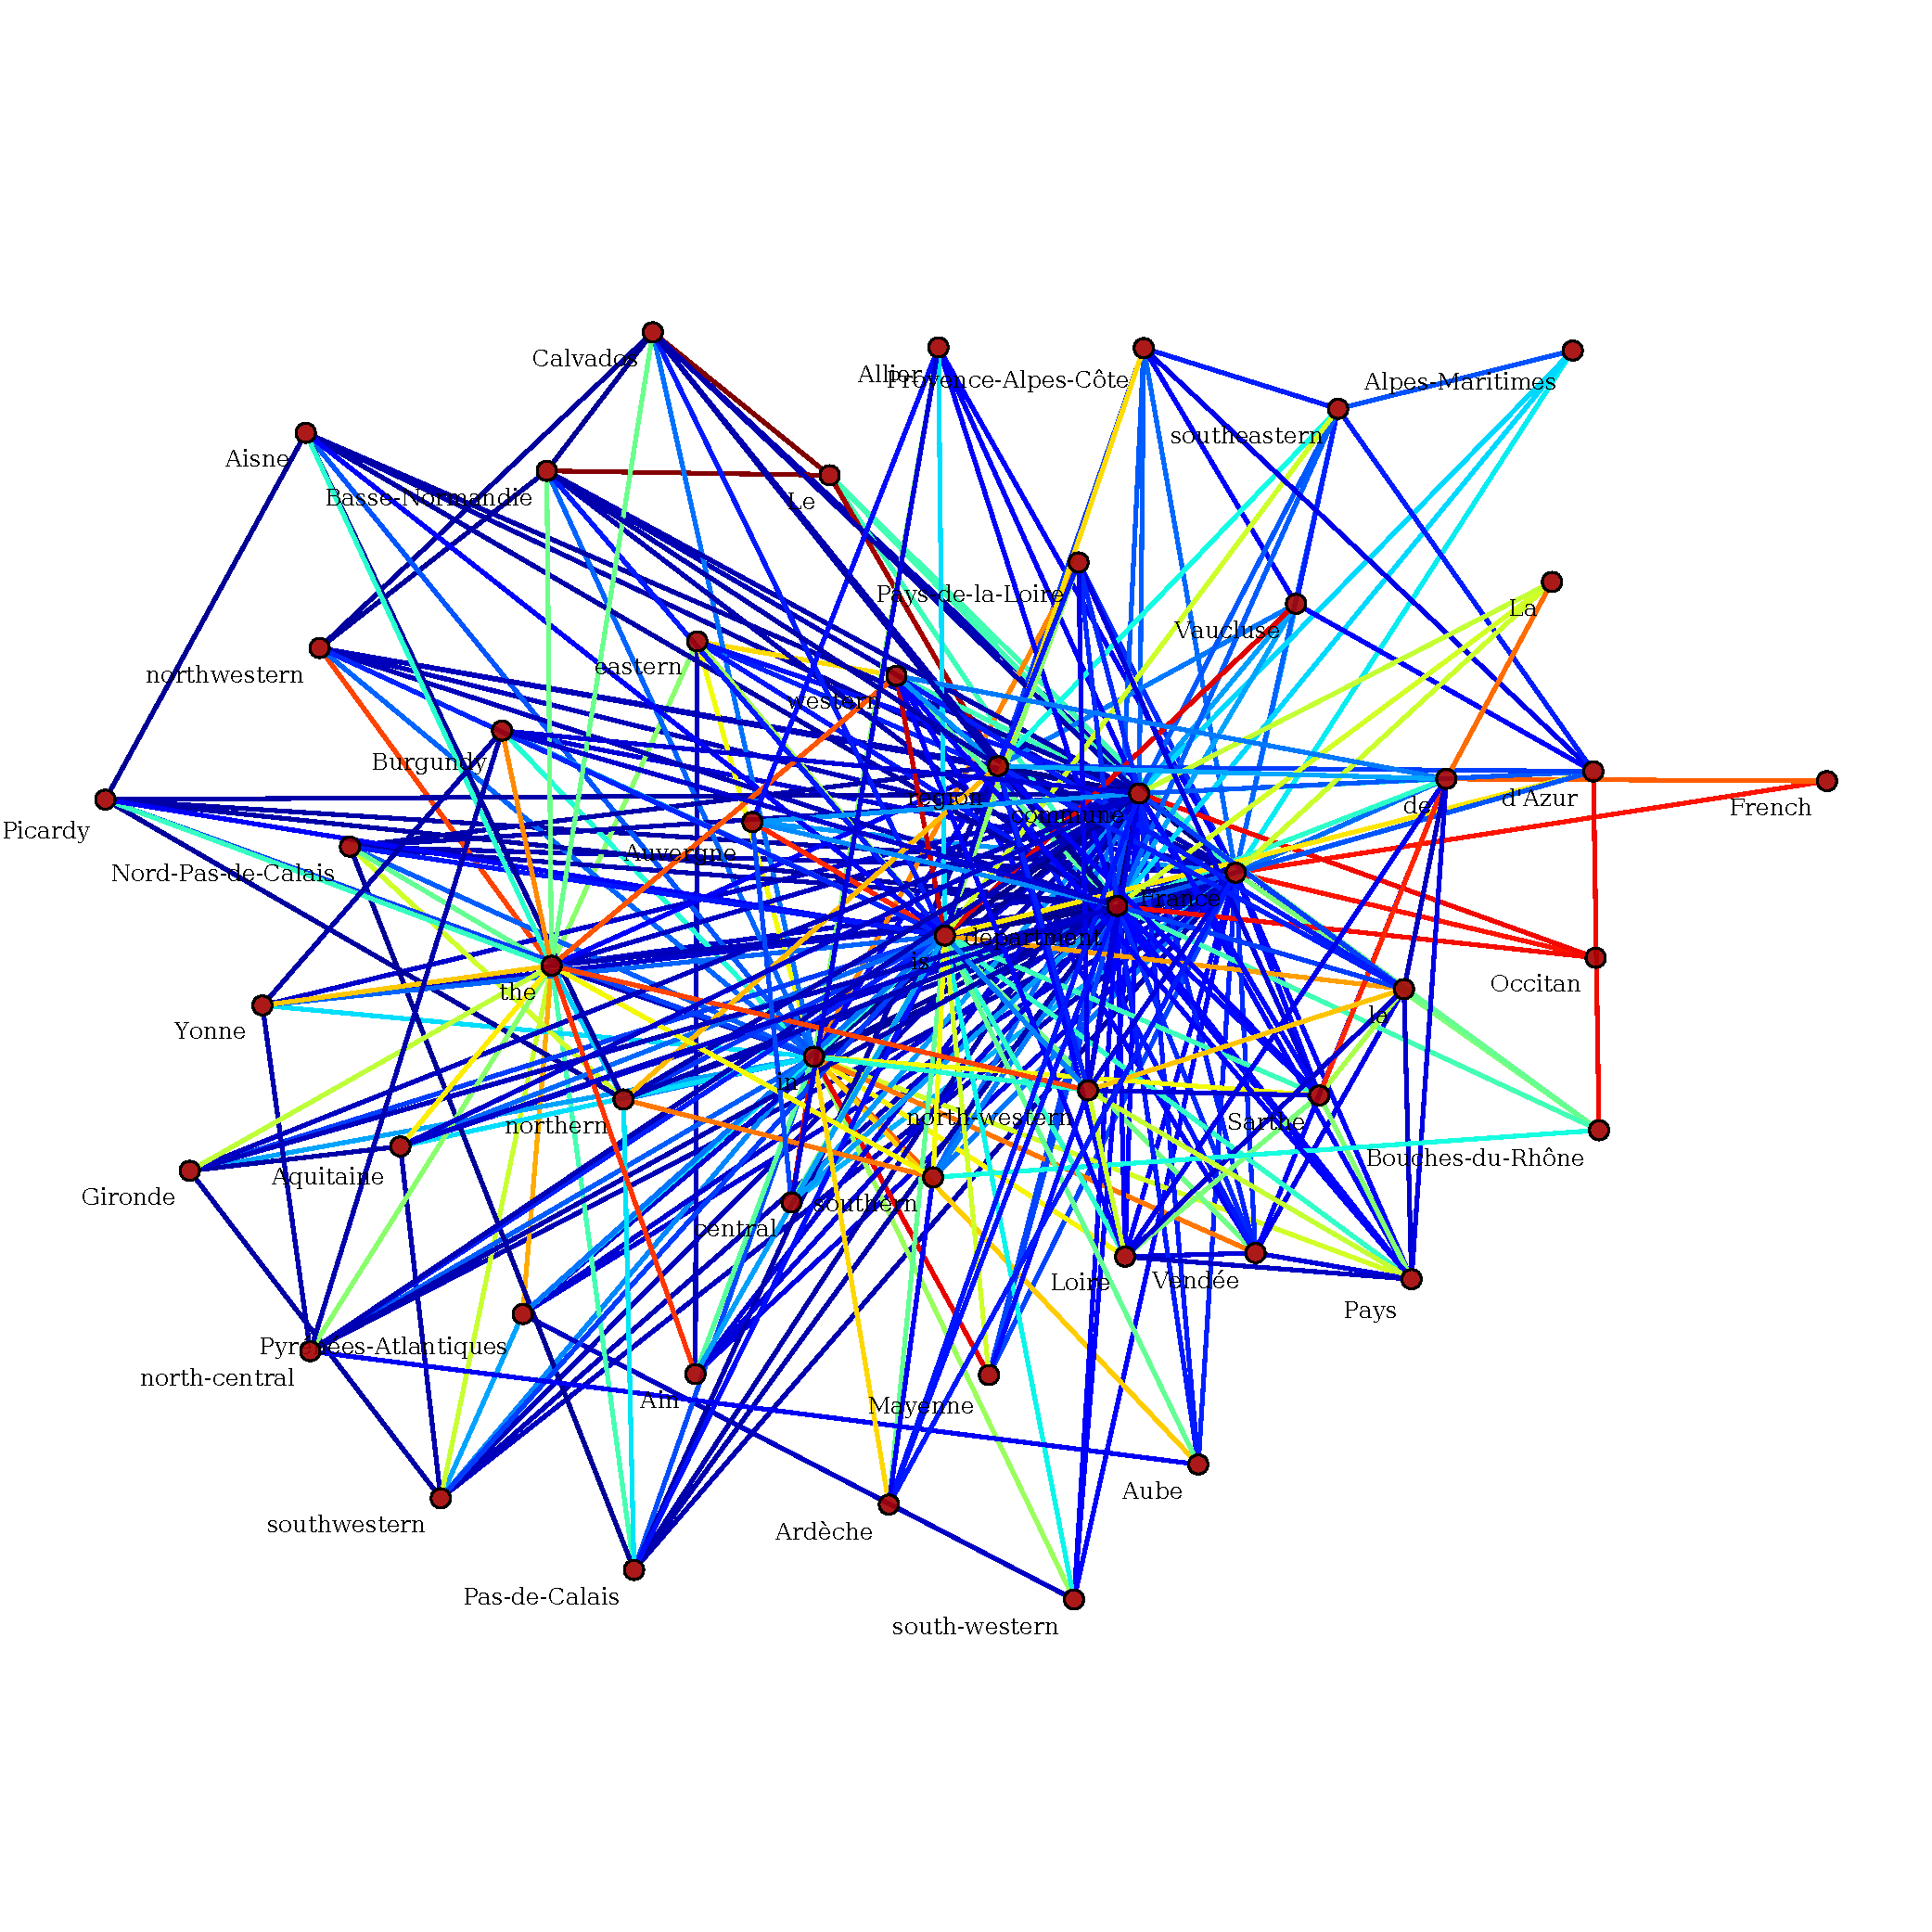
\includegraphics[scale=.25]{../../data/results/cooc_wiki_en/topwords-t0005/graph_France.pdf}
        \caption{Standard English, Häufigkeit 50}
    \end{subfigure}
    \caption{Kookkurrenzgraph France (Distanz 1, Schwellwert 0,005)}
    \label{fig:hw-france}
\end{figure}

\begin{figure}[hp!]
    \centering
    \begin{subfigure}[b]{0.5\textwidth}
        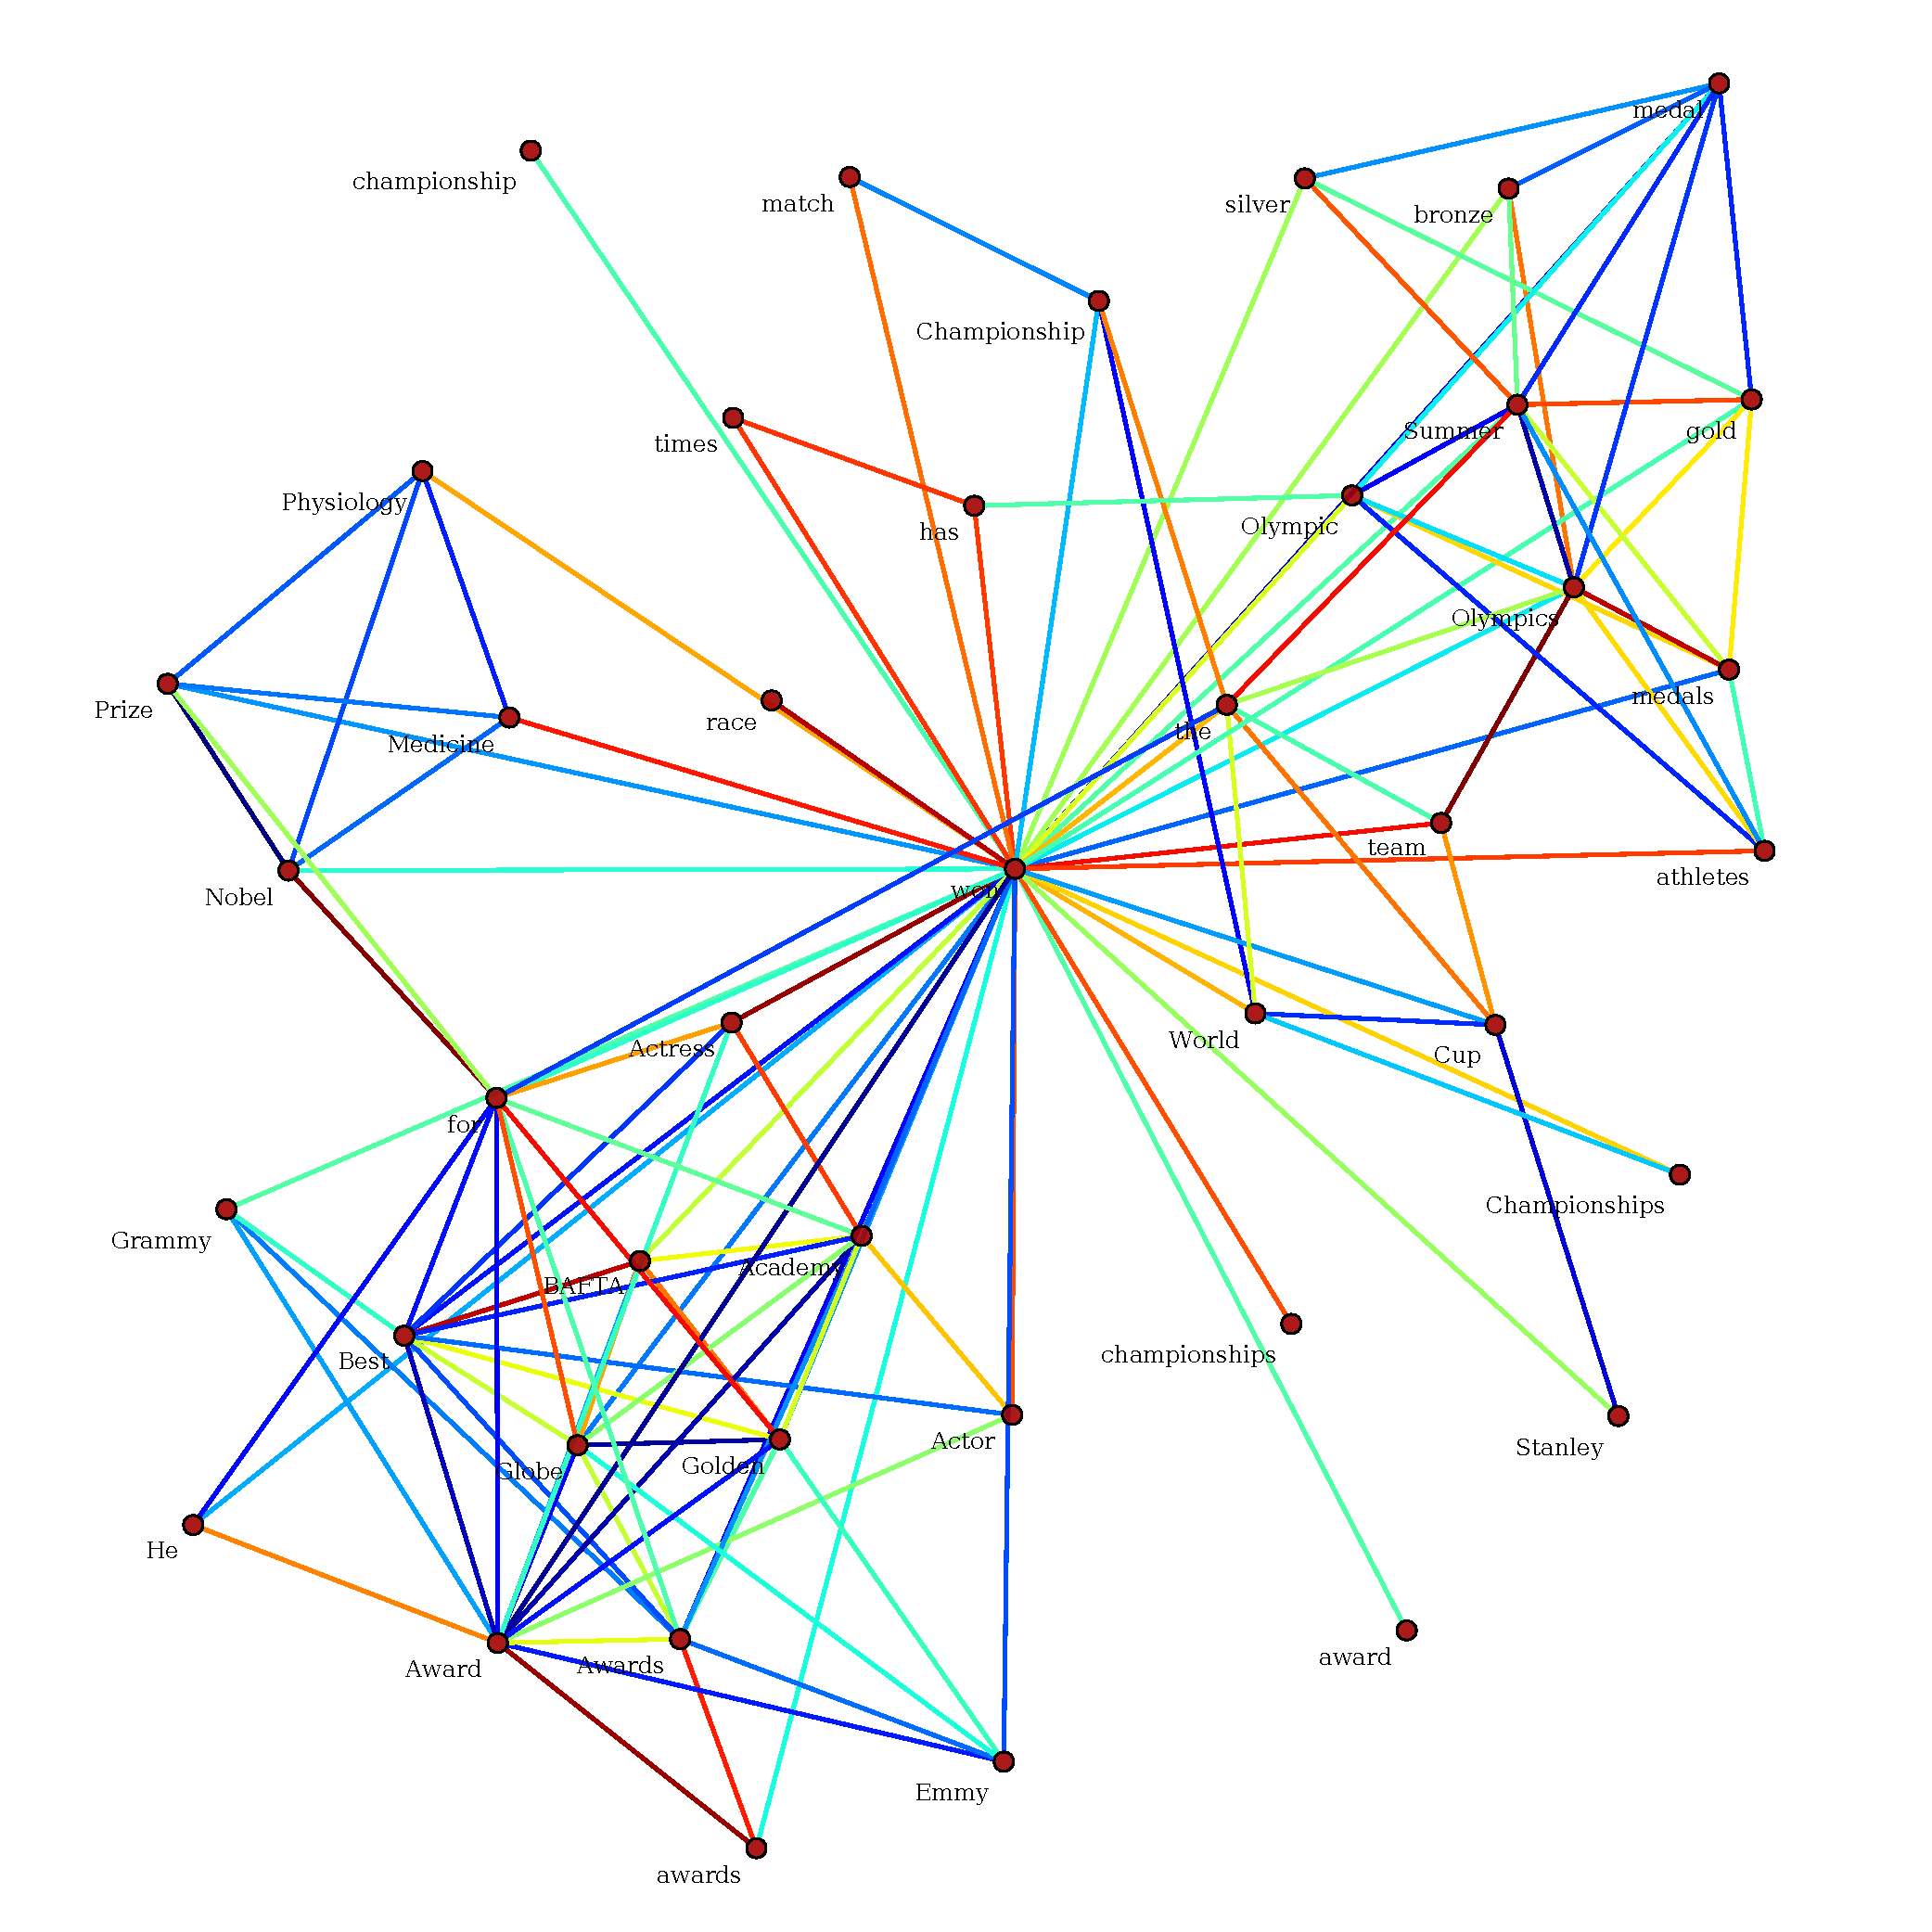
\includegraphics[scale=.25]{../../data/results/cooc_wiki_sim/topwords-t0005/graph_won.pdf}
        \caption{Simple English, Häufigkeit 41}
    \end{subfigure}
    \begin{subfigure}[b]{0.5\textwidth}
        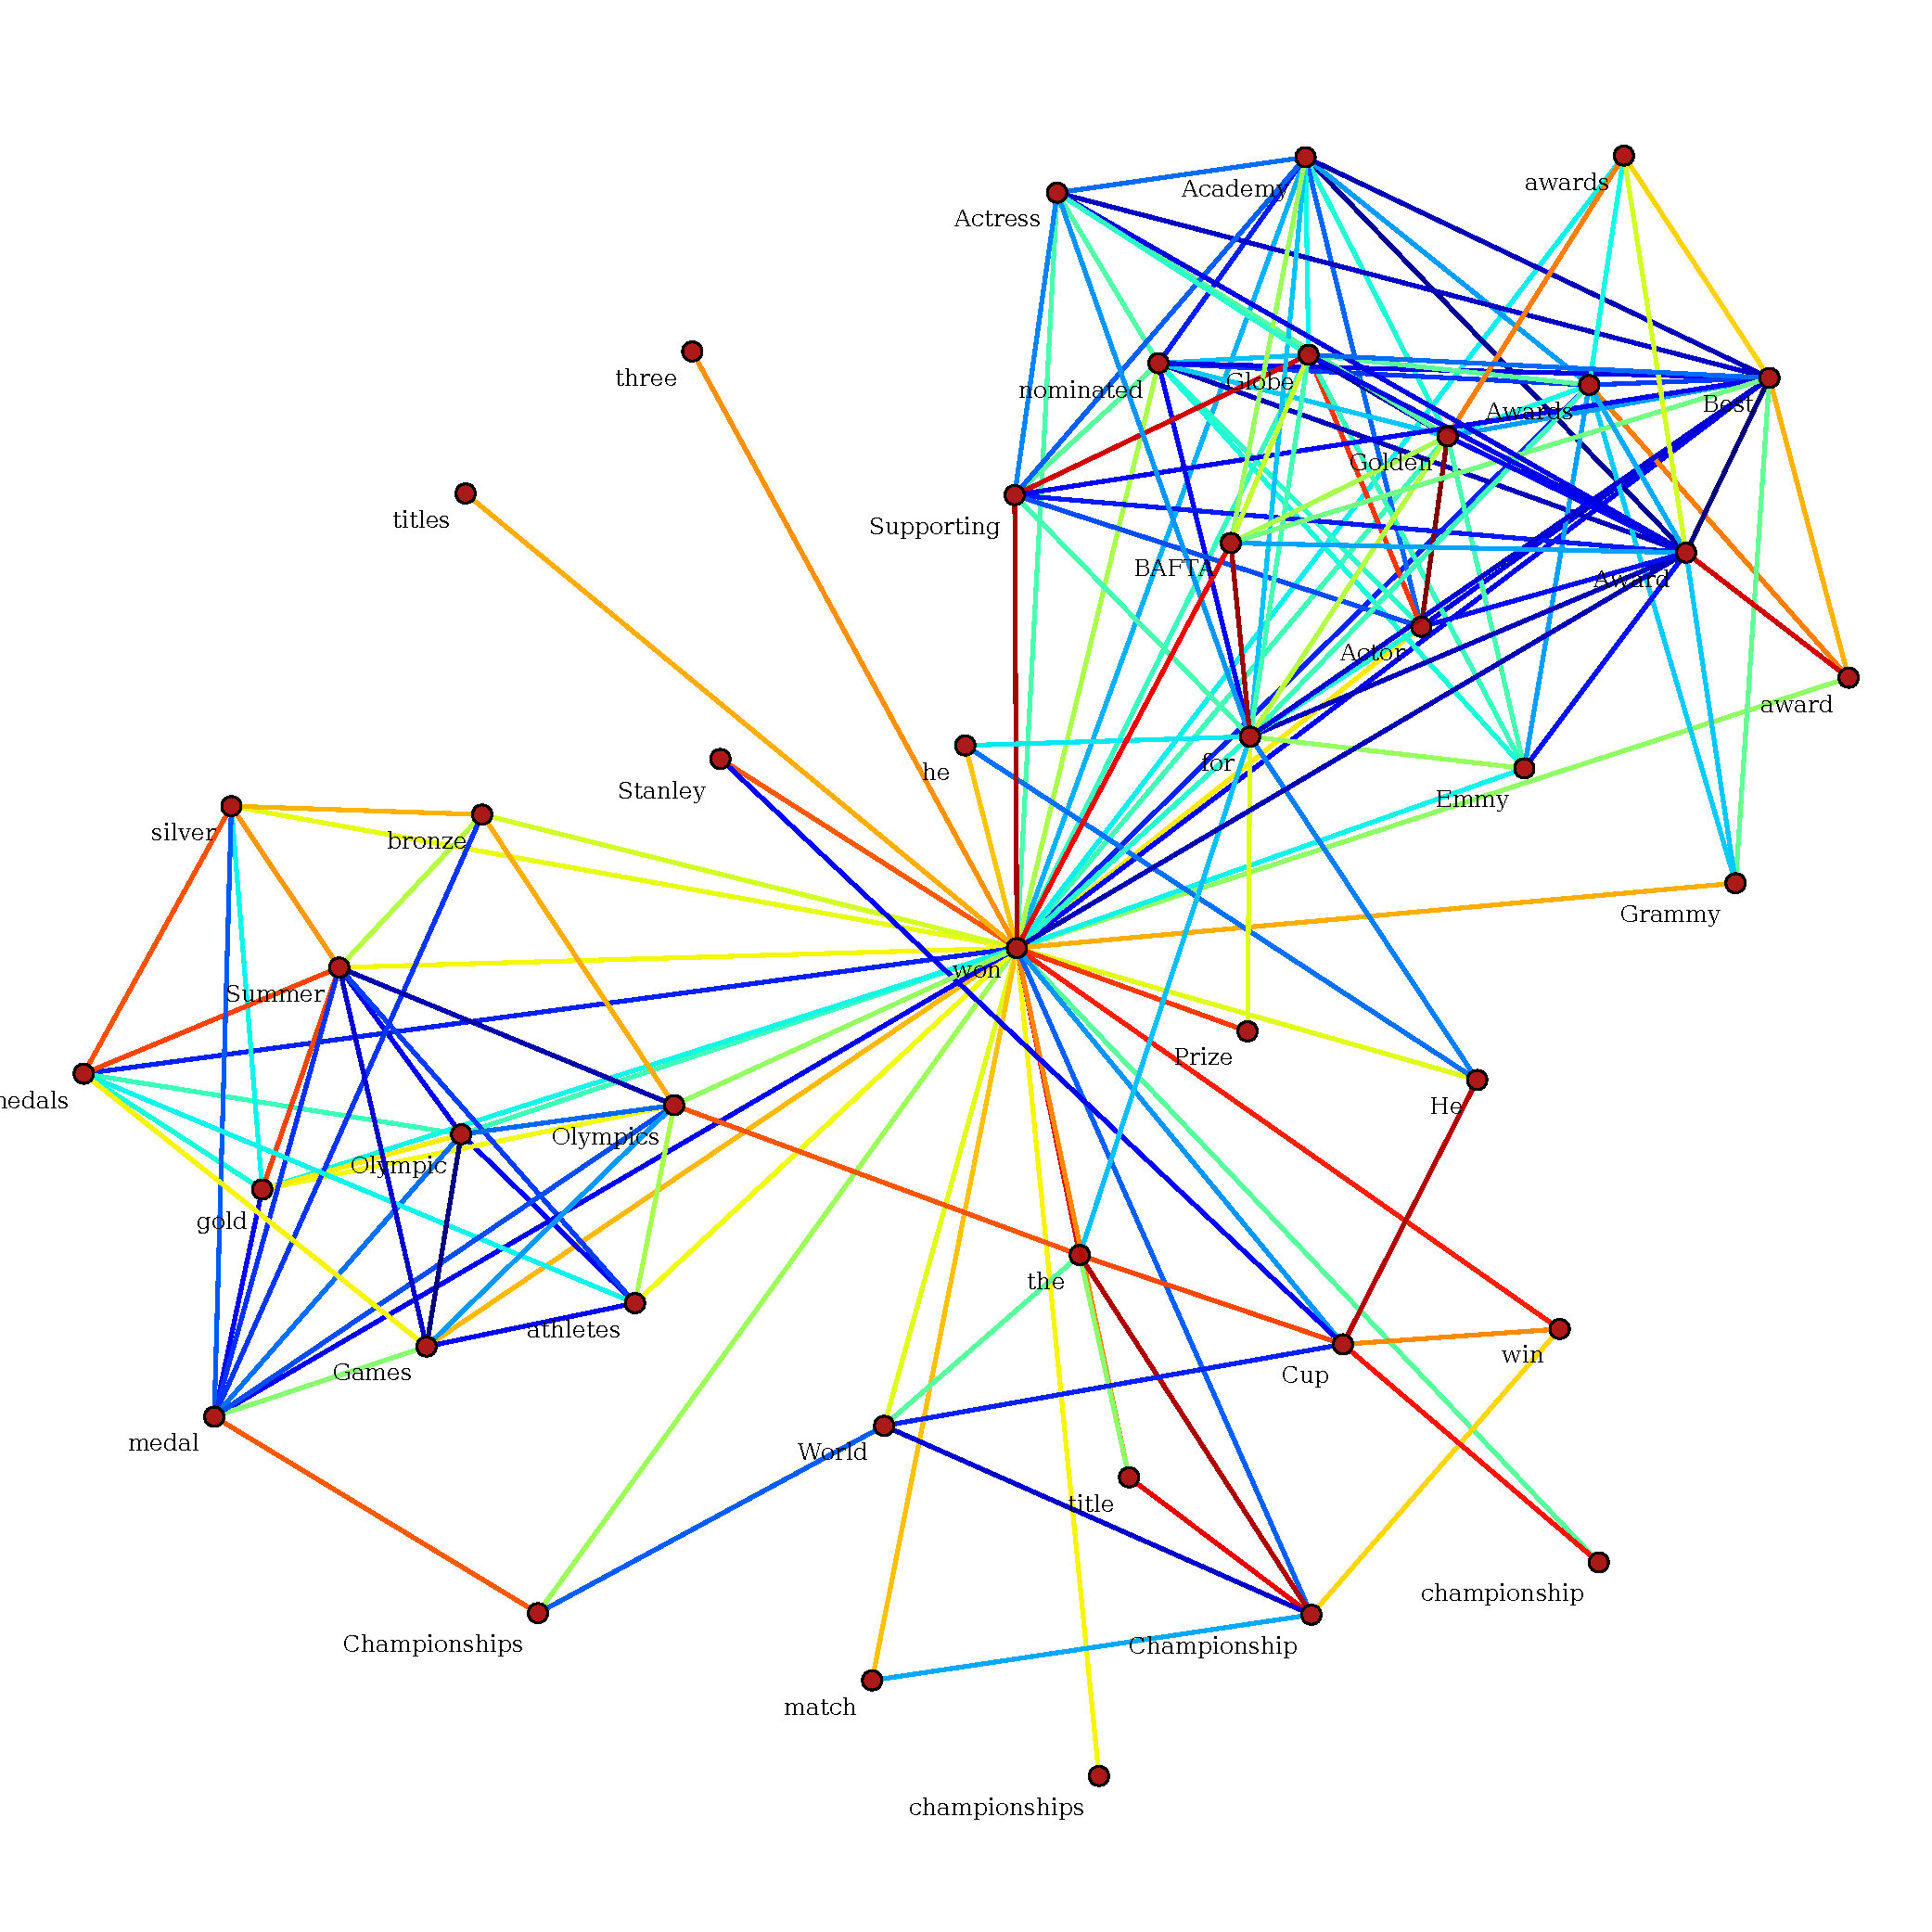
\includegraphics[scale=.25]{../../data/results/cooc_wiki_en/topwords-t0005/graph_won.pdf}
        \caption{Standard English, Häufigkeit 42}
    \end{subfigure}
    \caption{Kookkurrenzgraph won (Distanz 1, Schwellwert 0,005)}
    \label{fig:hw-won}
\end{figure}

\begin{figure}[hp!]
    \centering
    \begin{subfigure}[b]{0.5\textwidth}
        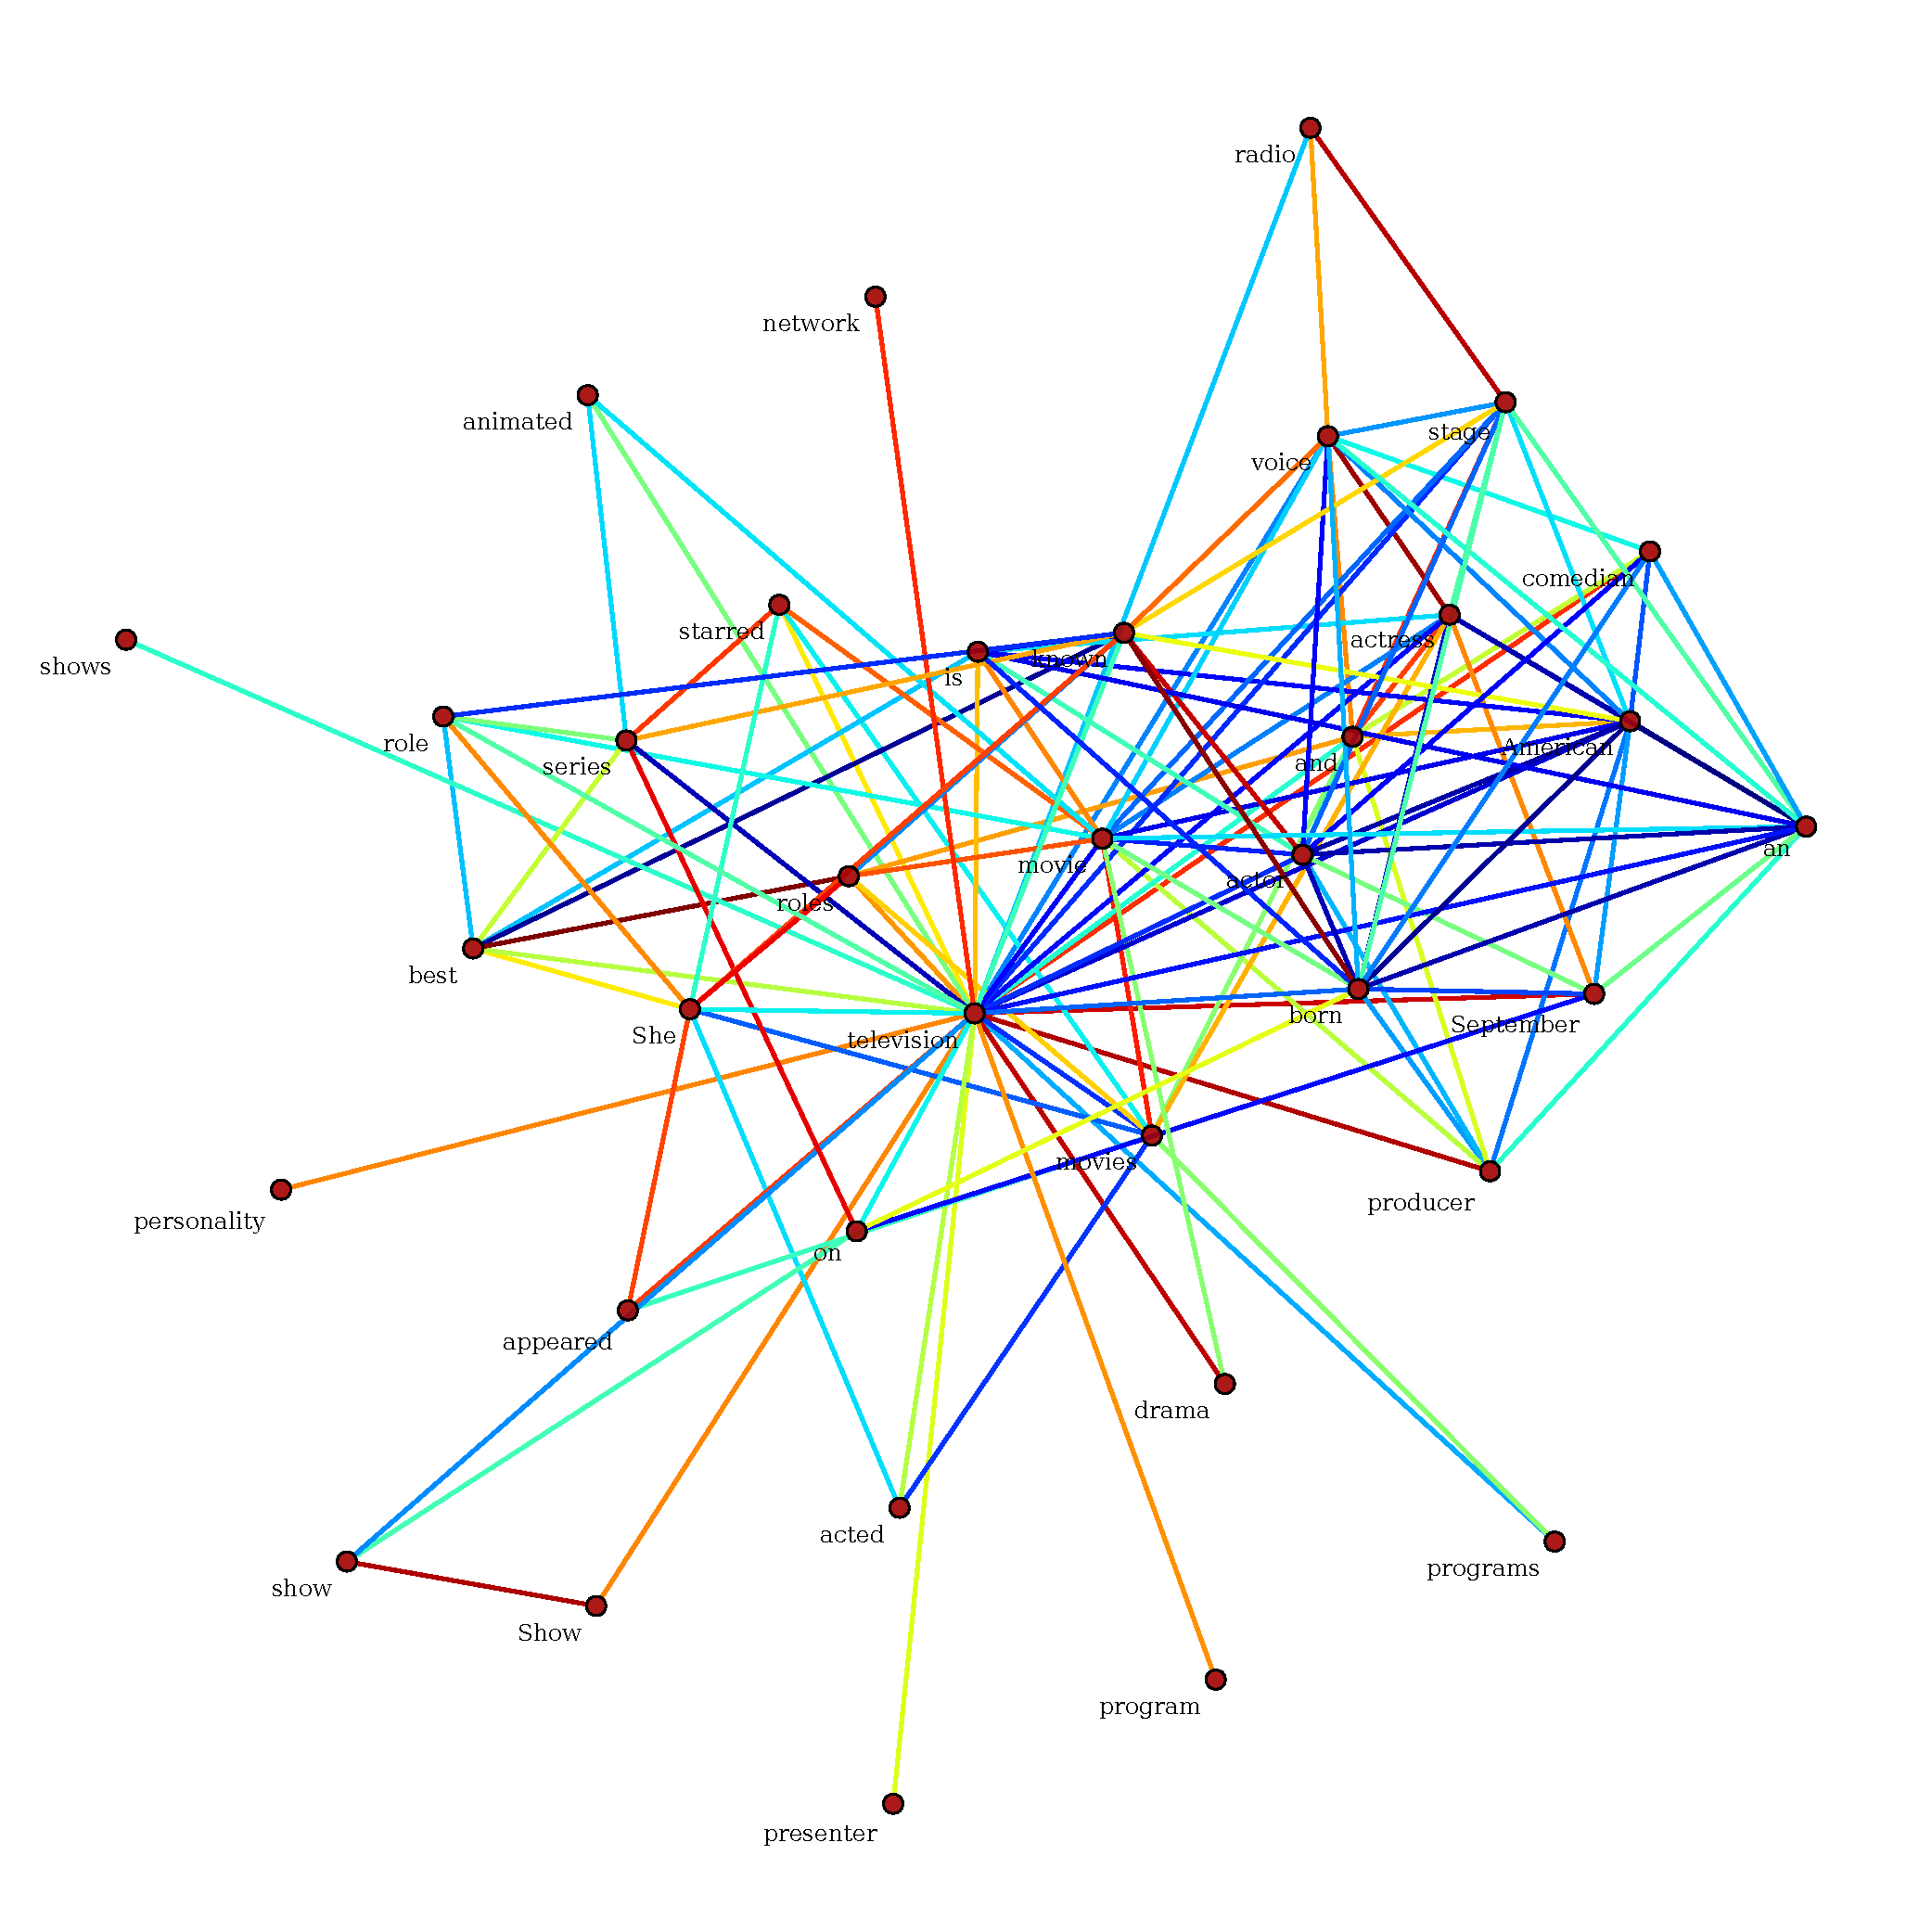
\includegraphics[scale=.25]{../../data/results/cooc_wiki_sim/topwords-t0005/graph_television.pdf}
        \caption{Simple English, Häufigkeit 35}
    \end{subfigure}
    \begin{subfigure}[b]{0.5\textwidth}
        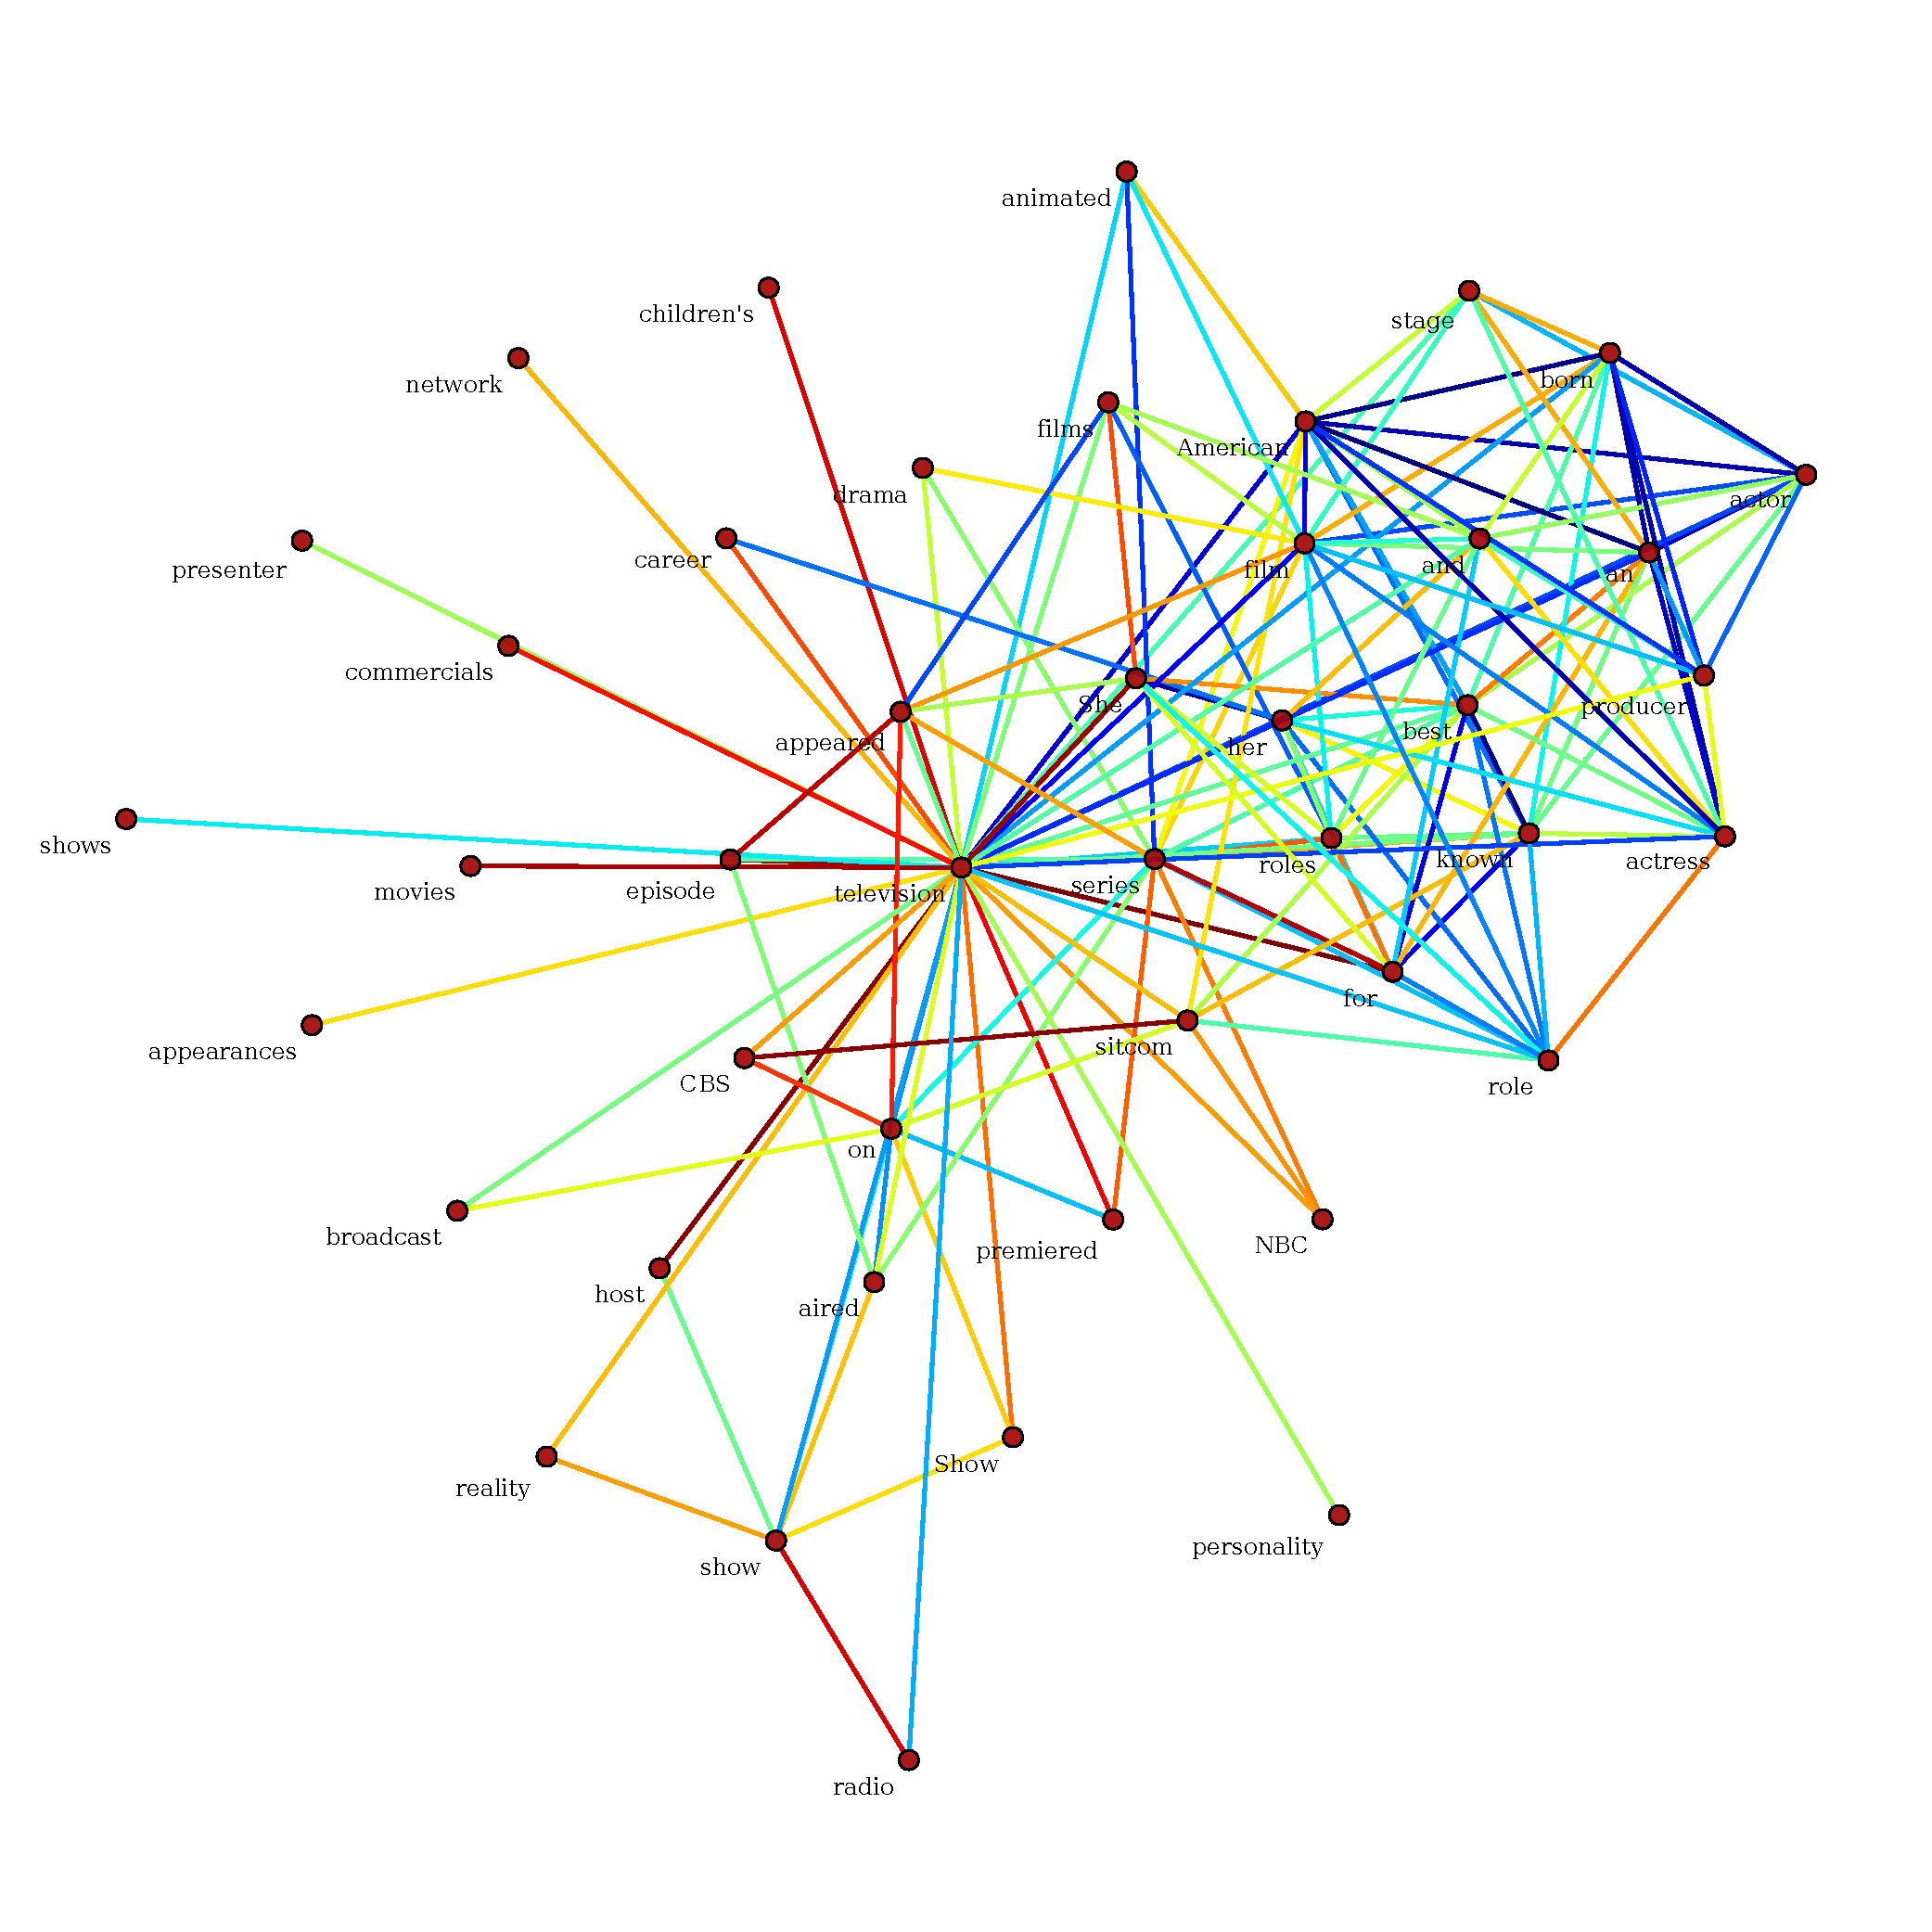
\includegraphics[scale=.25]{../../data/results/cooc_wiki_en/topwords-t0005/graph_television.pdf}
        \caption{Standard English, Häufigkeit 43}
    \end{subfigure}
    \caption{Kookkurrenzgraph television (Distanz 1, Schwellwert 0,005)}
    \label{fig:hw-television}
\end{figure}

\begin{figure}[hp!]
    \centering
    \begin{subfigure}[b]{0.5\textwidth}
        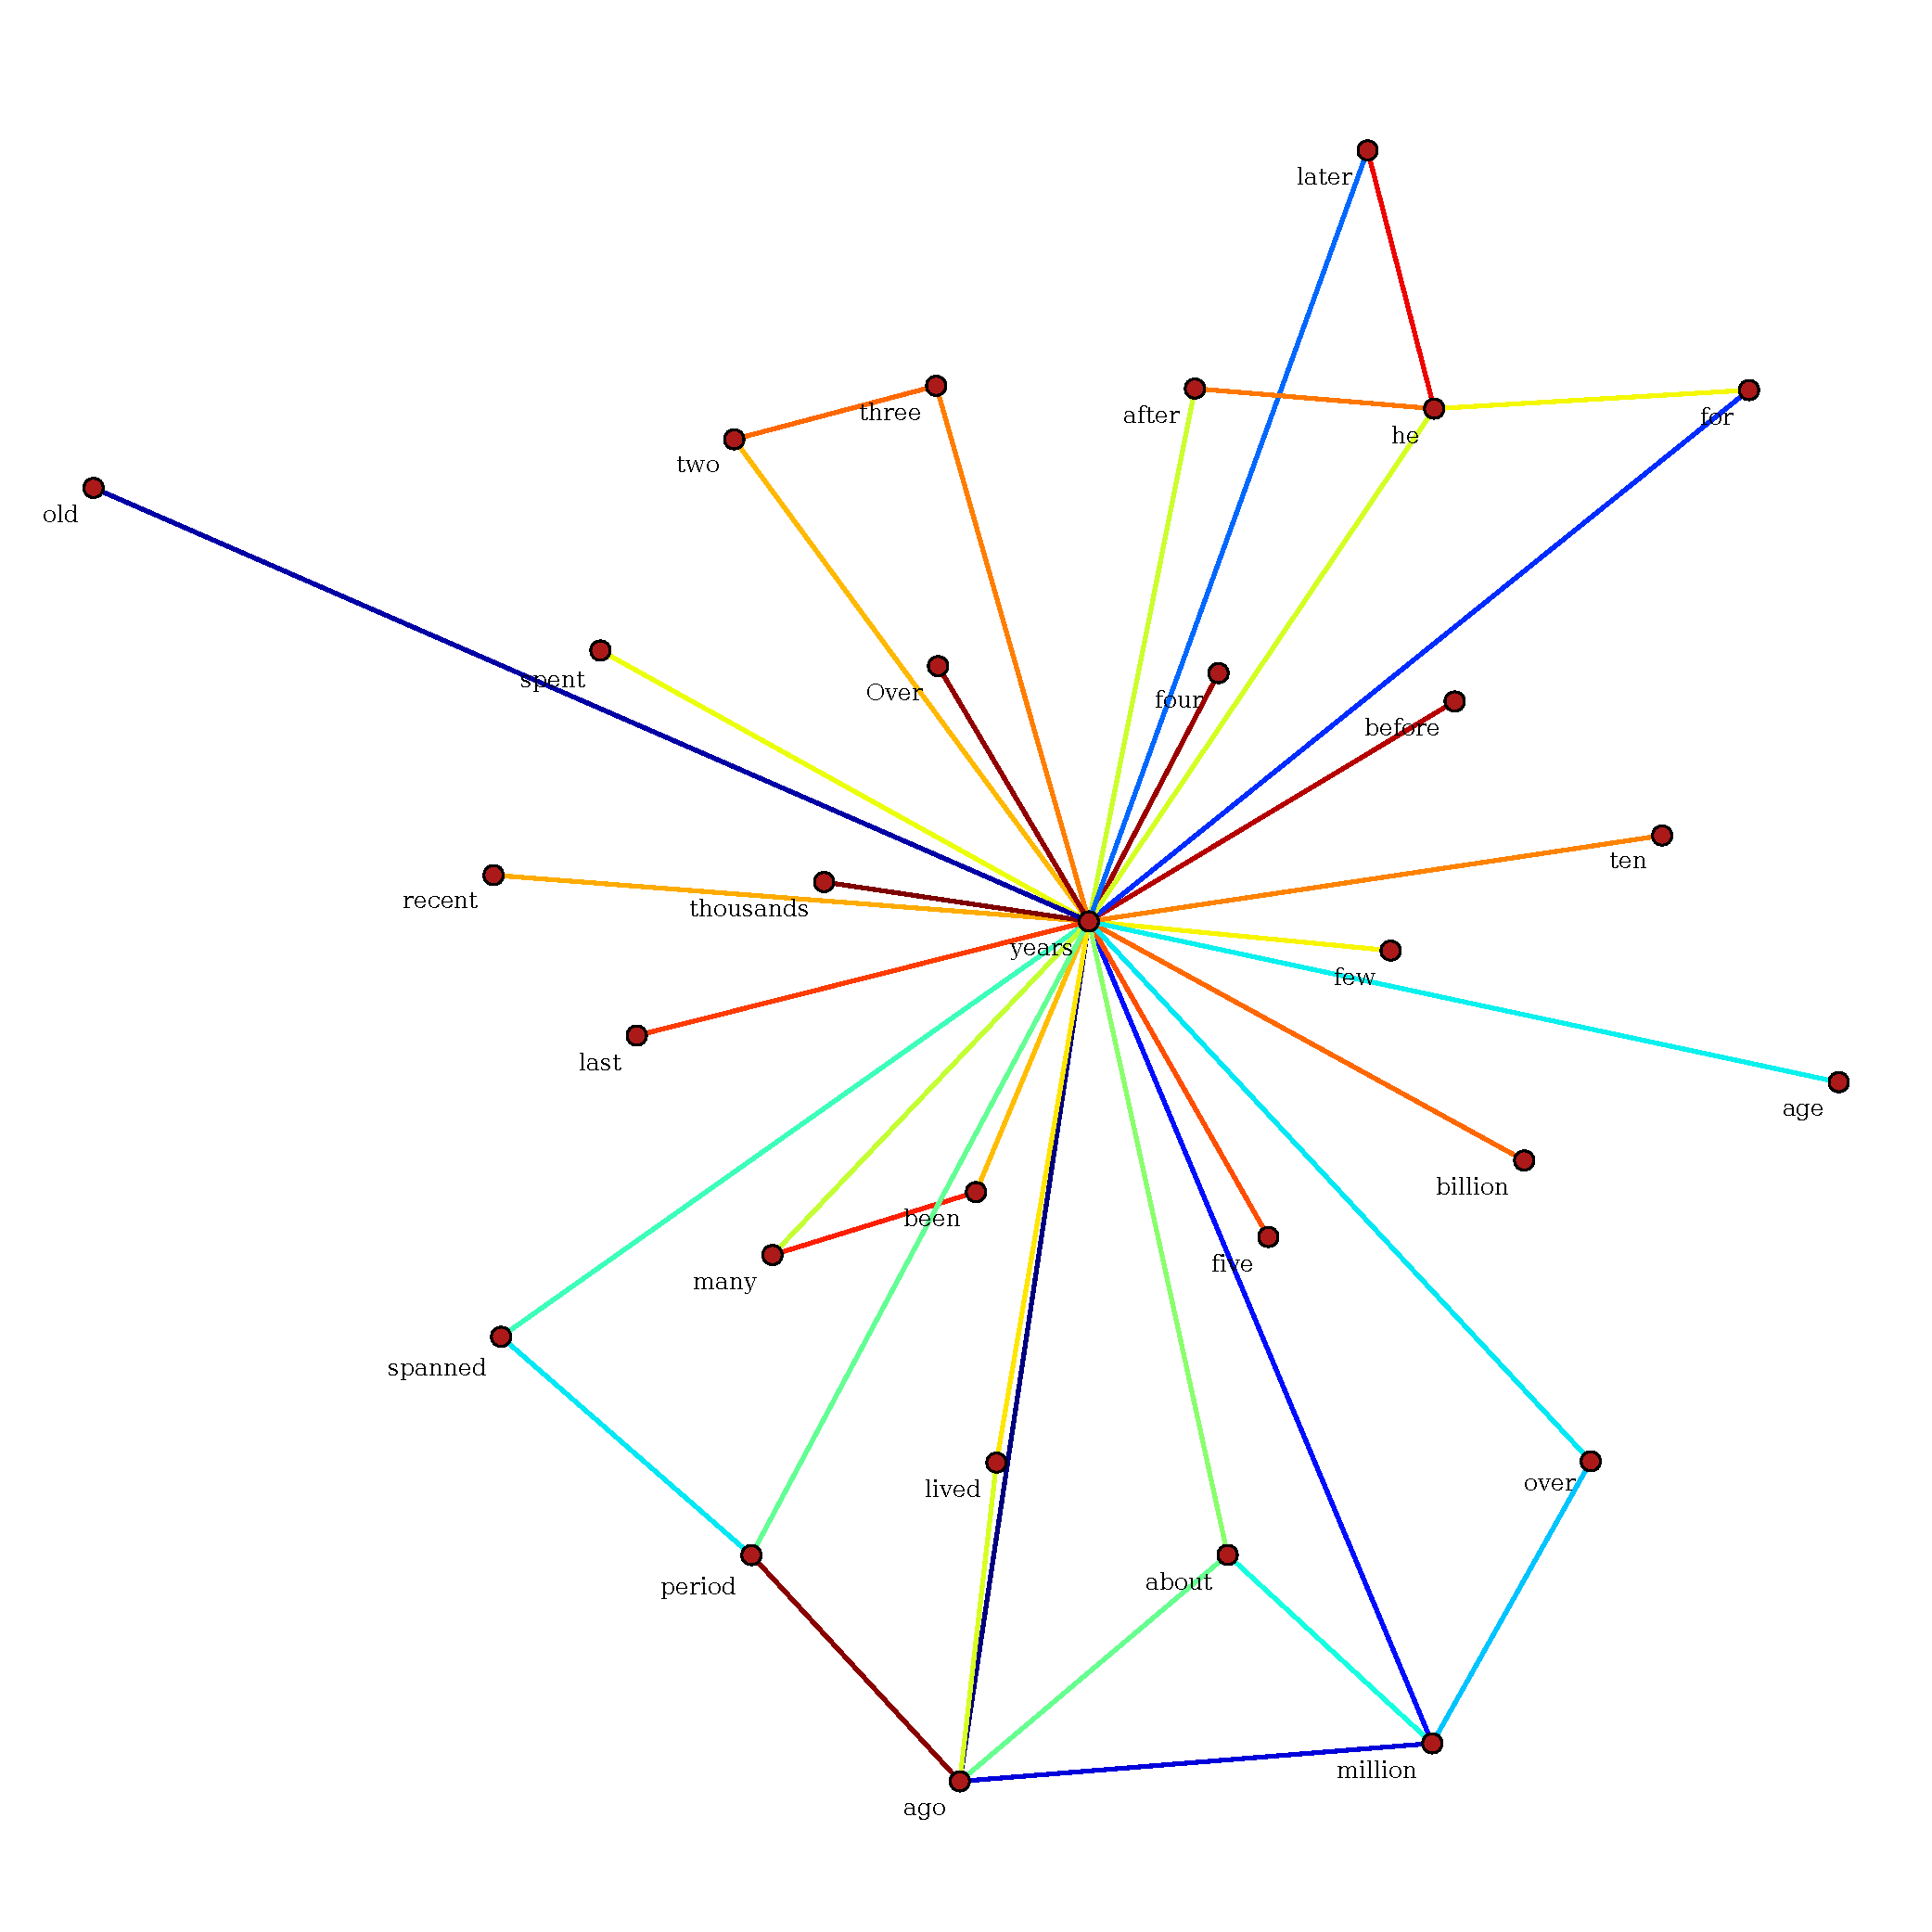
\includegraphics[scale=.25]{../../data/results/cooc_wiki_sim/topwords-t0005/graph_years.pdf}
        \caption{Simple English, Häufigkeit 28}
    \end{subfigure}
    \begin{subfigure}[b]{0.5\textwidth}
        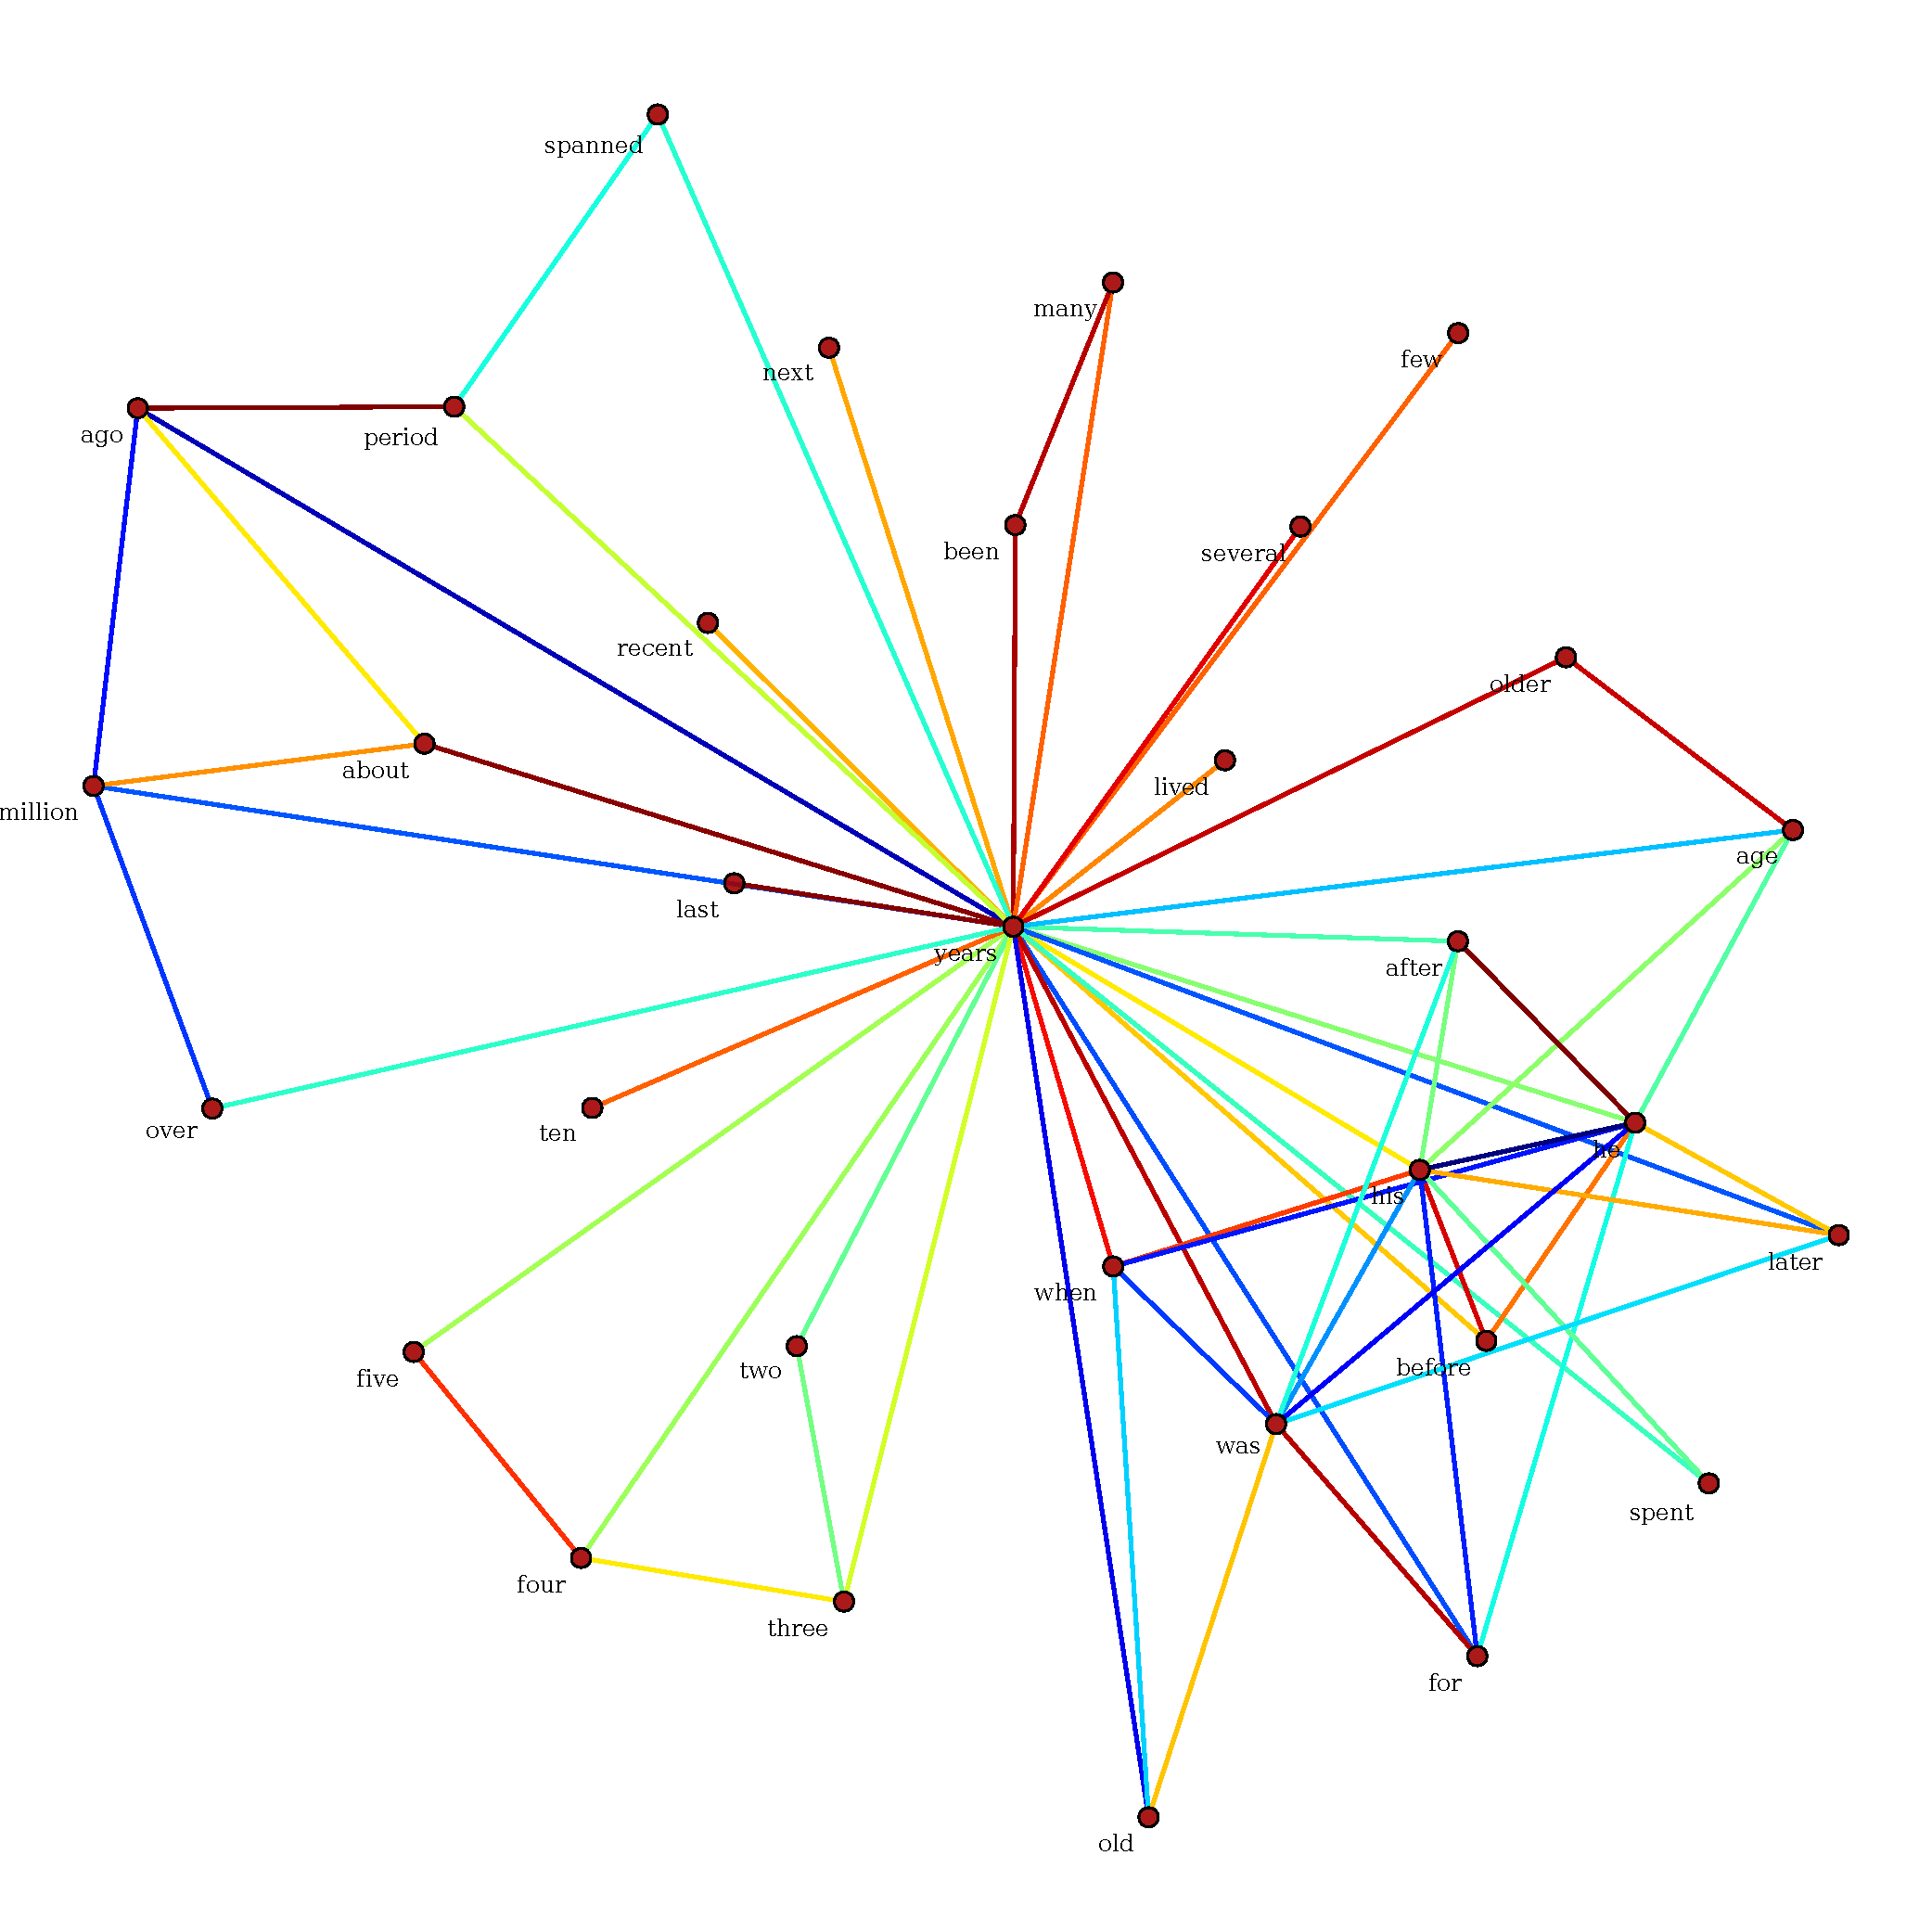
\includegraphics[scale=.25]{../../data/results/cooc_wiki_en/topwords-t0005/graph_years.pdf}
        \caption{Standard English, Häufigkeit 31}
    \end{subfigure}
    \caption{Kookkurrenzgraph years (Distanz 1, Schwellwert 0,005)}
    \label{fig:hw-years}
\end{figure}


\pagebreak
\subsection{Weit außen liegende Wörter}
\label{sec:aussen_liegende}

Zur Erstellung dieser Subgraphen wurden weit außen liegende Wörter ermittelt,
d.h. solche Wörter, von denen die längsten Pfade im Graphen ausgehen.

Zusätzlich zum Kookkurrenz-Schwellwert wurde hier bei der Graphenerzeugung
die Knotendistanz variiert, d.h. die Anzahl der `hops' ausgehend vom Zielwort,
die in den Graphen mit einbezogen werden (und deren evtl. auftretende
Querverbindungen untereinander).
Eine Distanz von 1 bedeutet, dass nur die direkten Nachbarn (und evtl.
auftretende Querverbindungen) einbezogen werden, bei kommen 2 zusätzlich deren
Nachbarn hinzu, usw.

Auch hier sind die jeweiligen Parameter in der Legende der Grafik angegeben.

\subsubsection{nachrichtenleicht.de}

\begin{figure}[hp!]
    \centering
        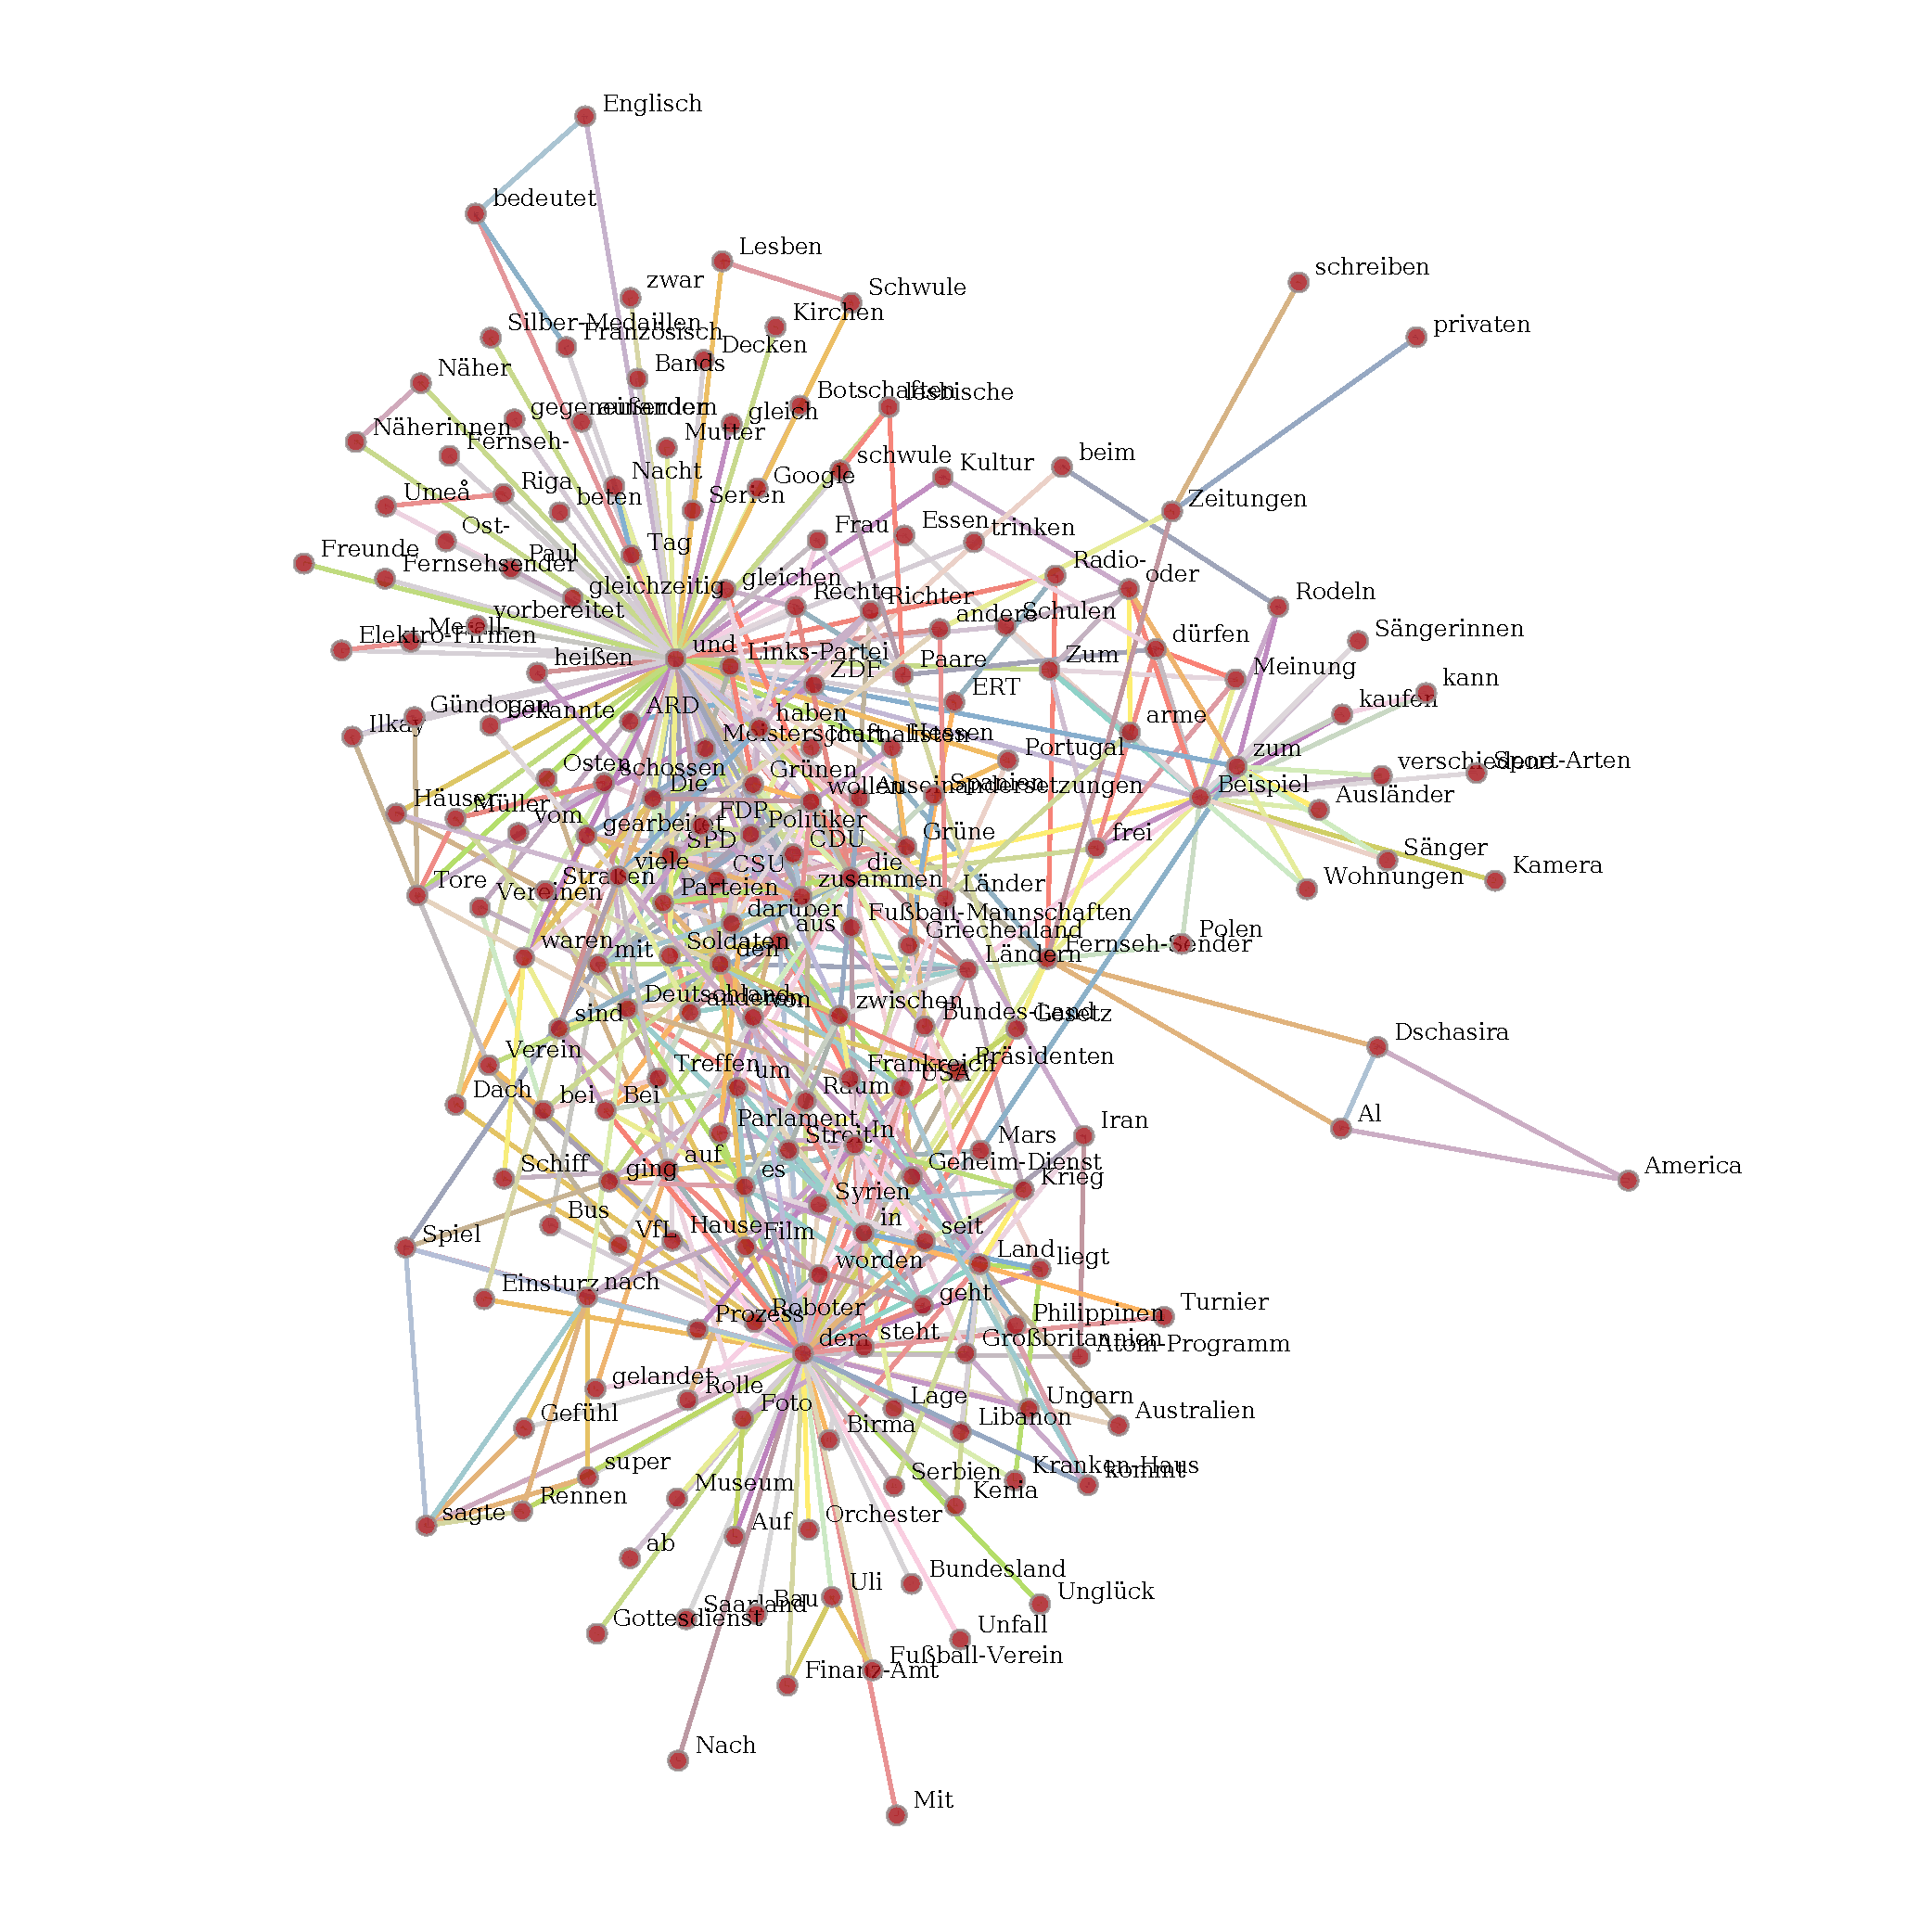
\includegraphics[scale=.4]{../../data/results/longpath_wordgraphs/nl/graph_America.pdf}
    \caption{Kookkurrenzgraph America (Distanz 4, Schwellwert 0,1)}
    \label{fig:lp-america}
\end{figure}

\begin{figure}[hp!]
    \centering
        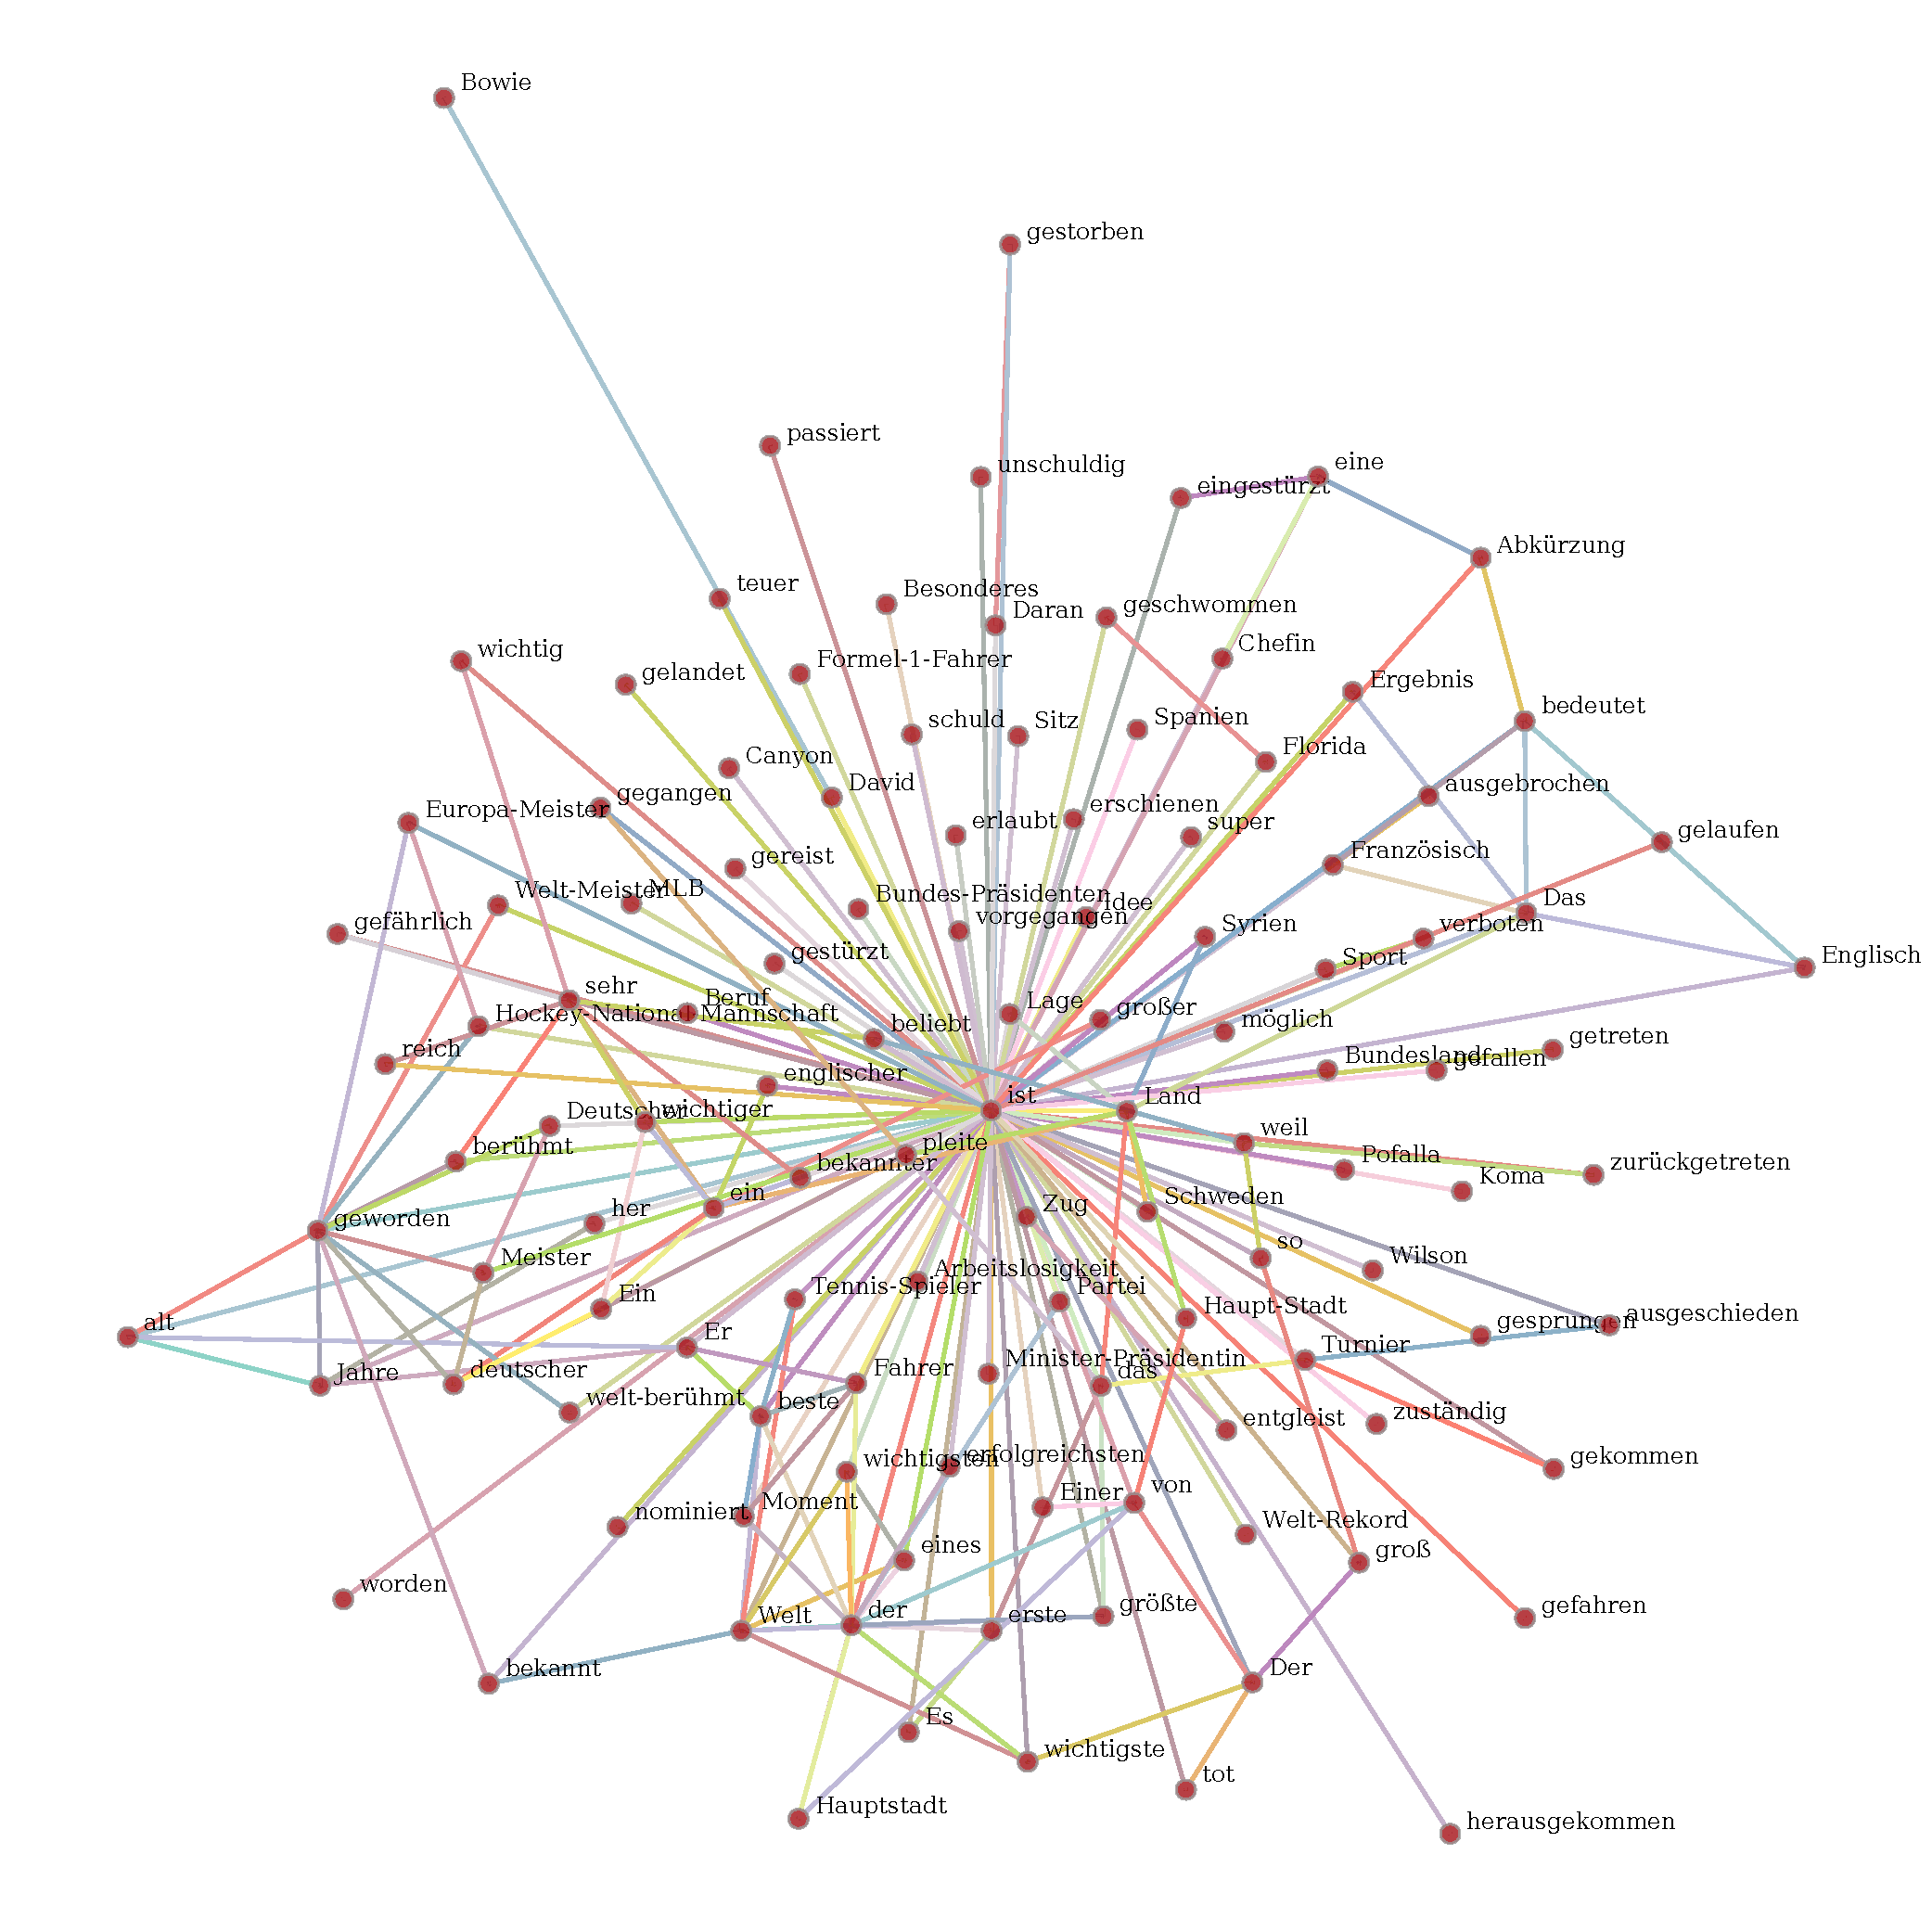
\includegraphics[scale=.4]{../../data/results/longpath_wordgraphs/nl/graph_Bowie.pdf}
    \caption{Kookkurrenzgraph Bowie (Distanz 3, Schwellwert 0,12)}
    \label{fig:lp-bowie}
\end{figure}

\begin{figure}[hp!]
    \centering
        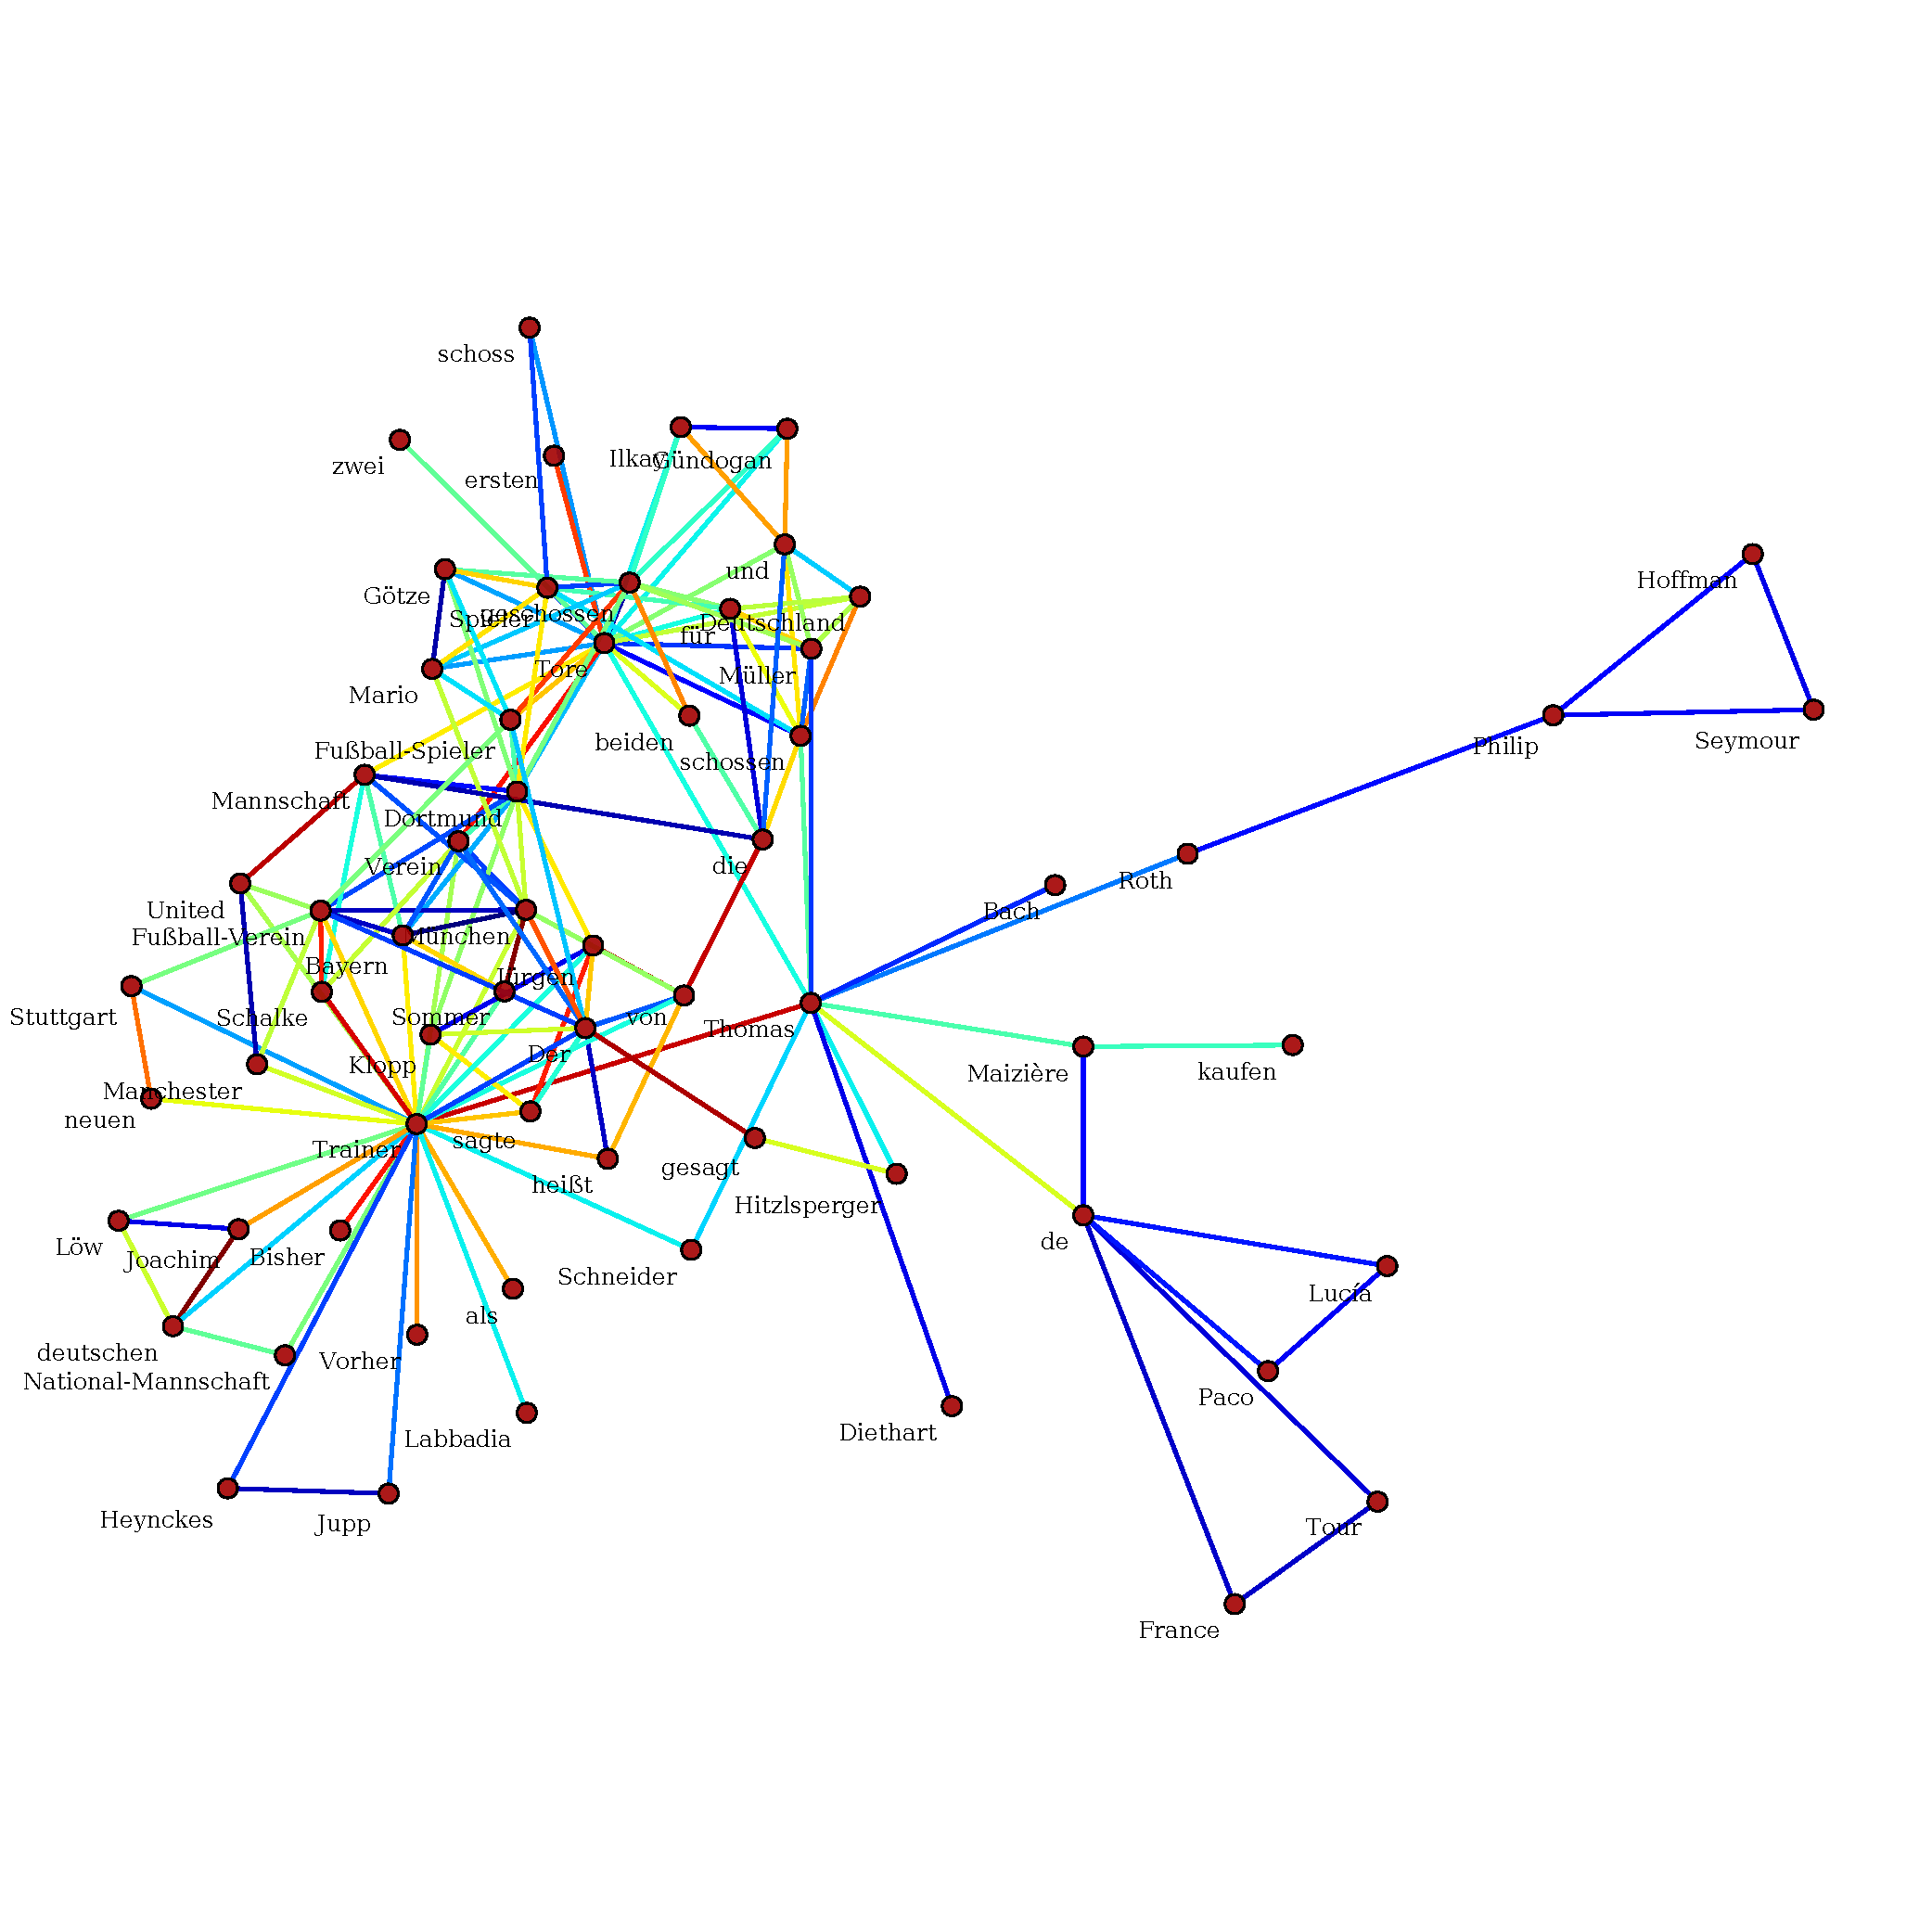
\includegraphics[scale=.4]{../../data/results/longpath_wordgraphs/nl/graph_Hoffman.pdf}
    \caption{Kookkurrenzgraph Hoffman (Distanz 5, Schwellwert 0,1)}
    \label{fig:lp-hoffman}
\end{figure}

\begin{figure}[hp!]
    \centering
        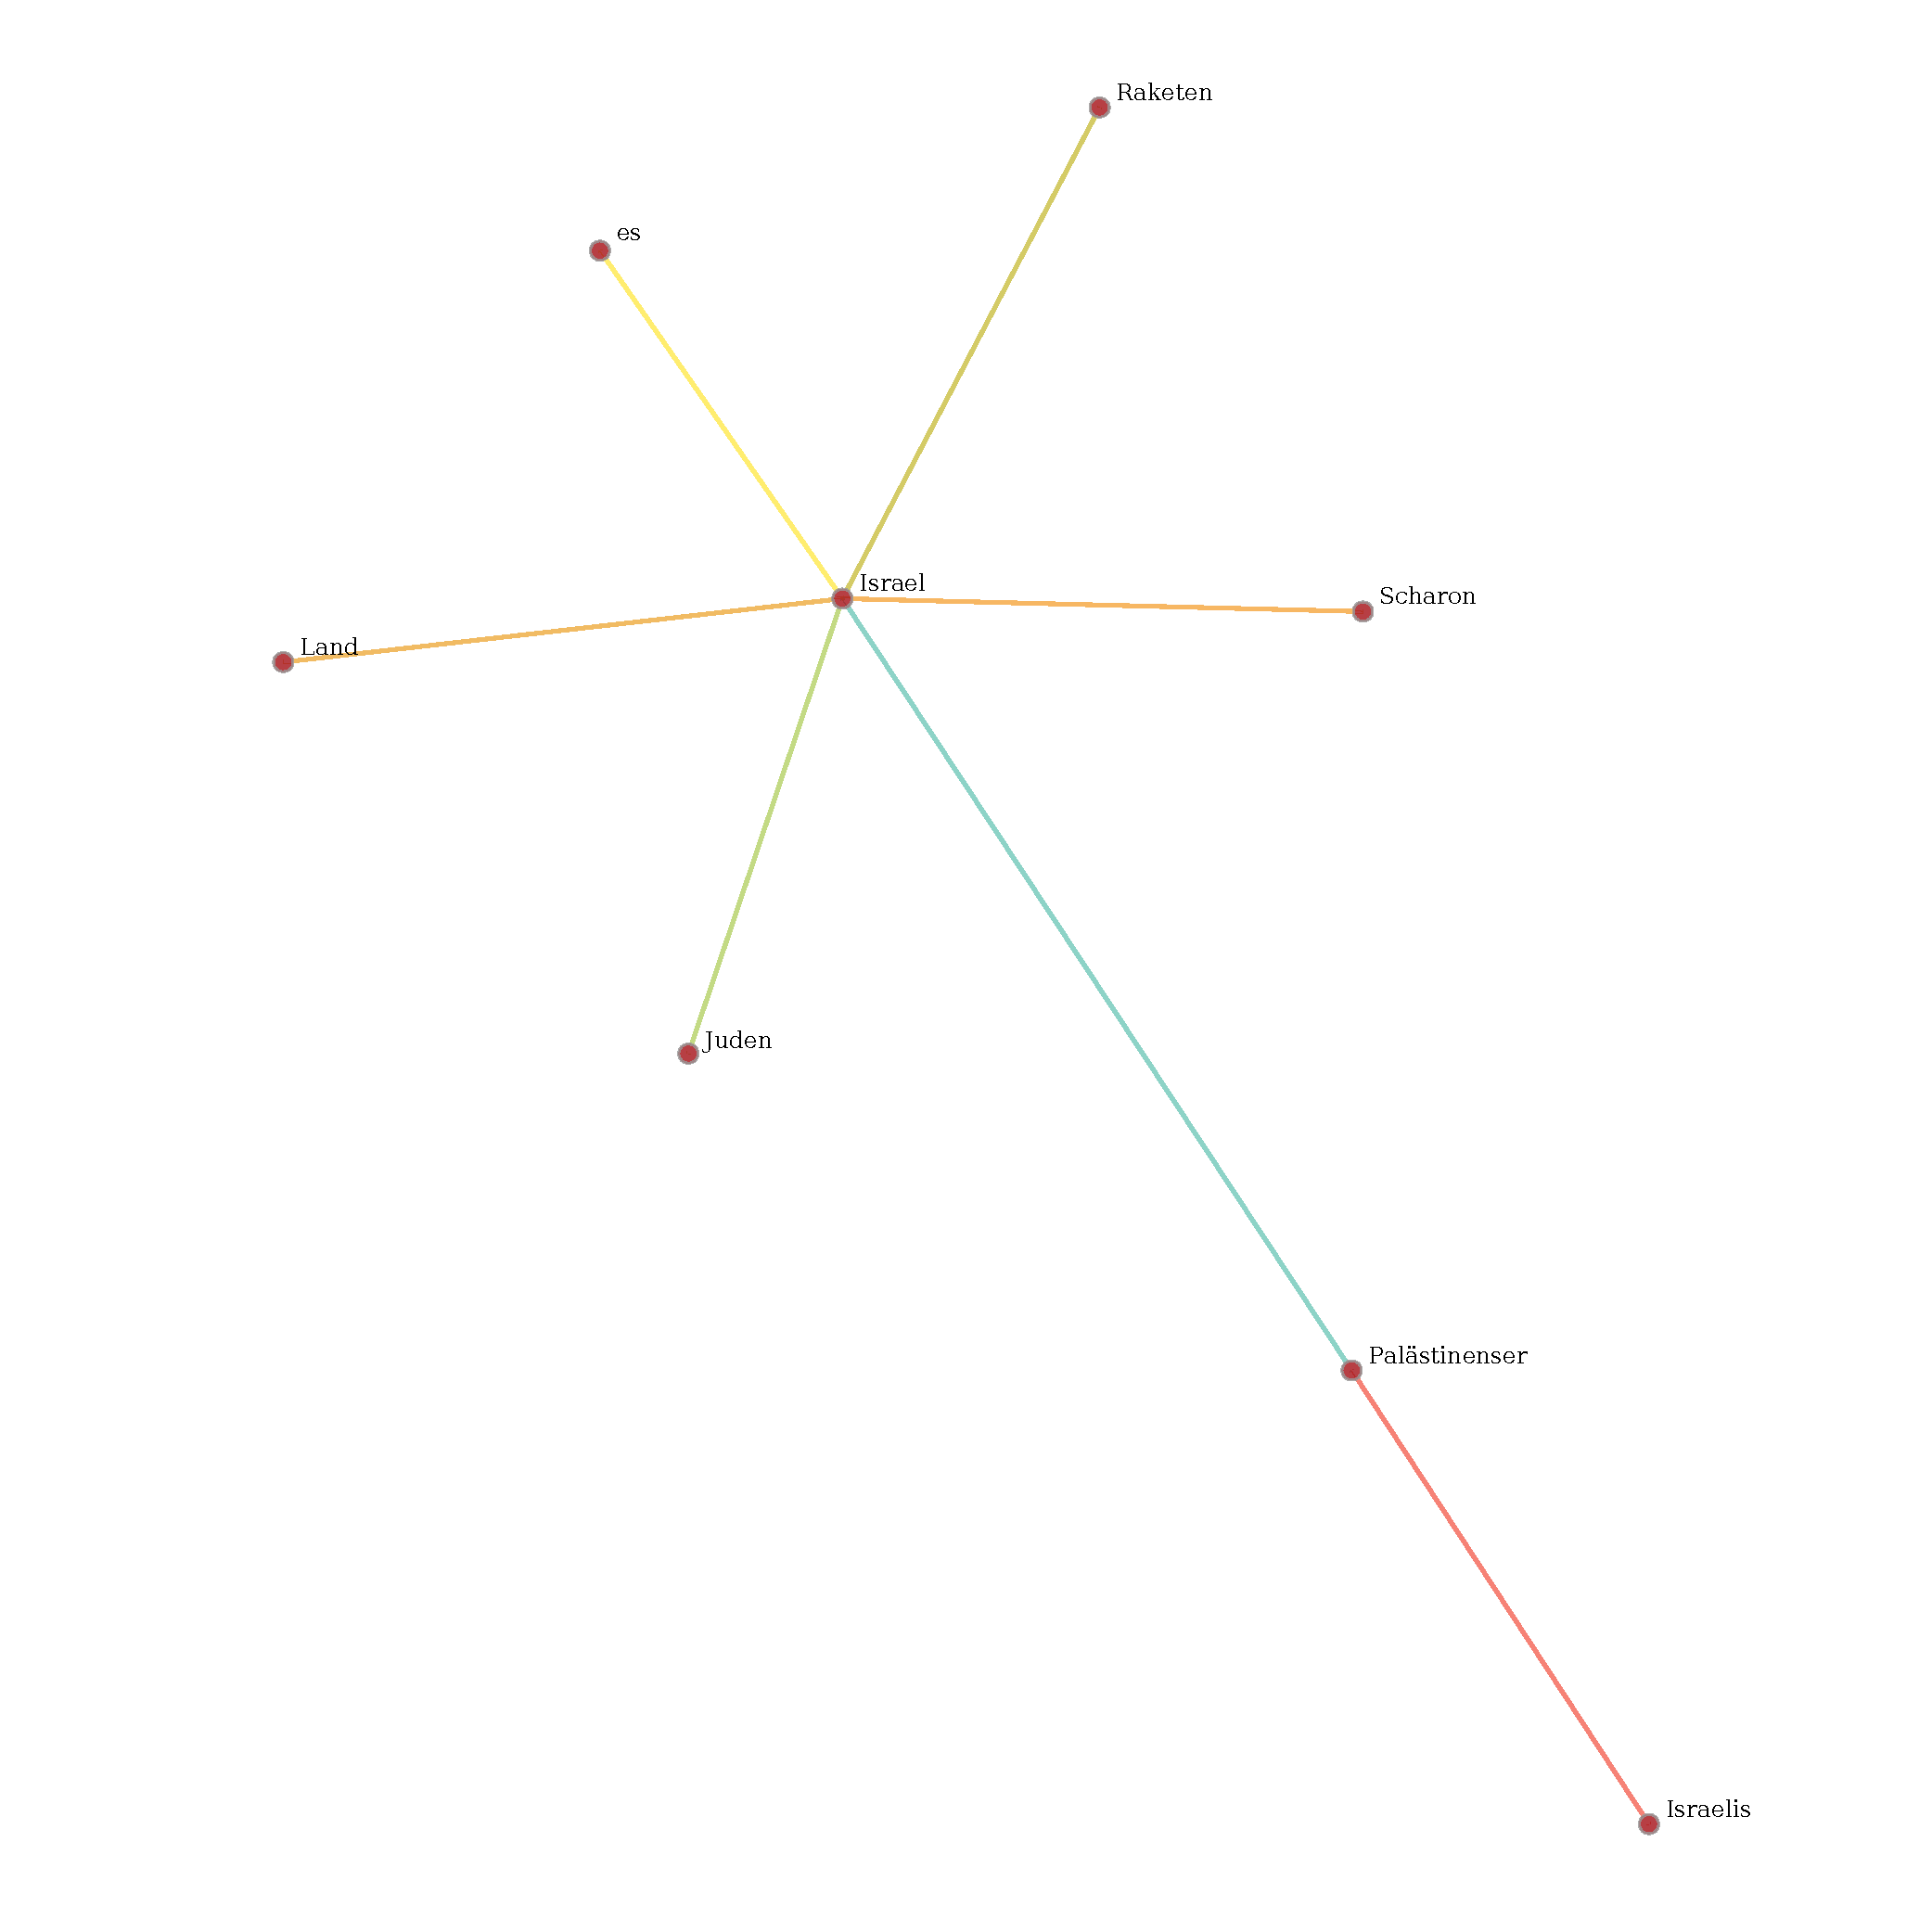
\includegraphics[scale=.4]{../../data/results/longpath_wordgraphs/nl/graph_Israelis.pdf}
    \caption{Kookkurrenzgraph Israelis (Distanz 3, Schwellwert 0,1)}
    \label{fig:lp-israelis}
\end{figure}

\begin{figure}[hp!]
    \centering
        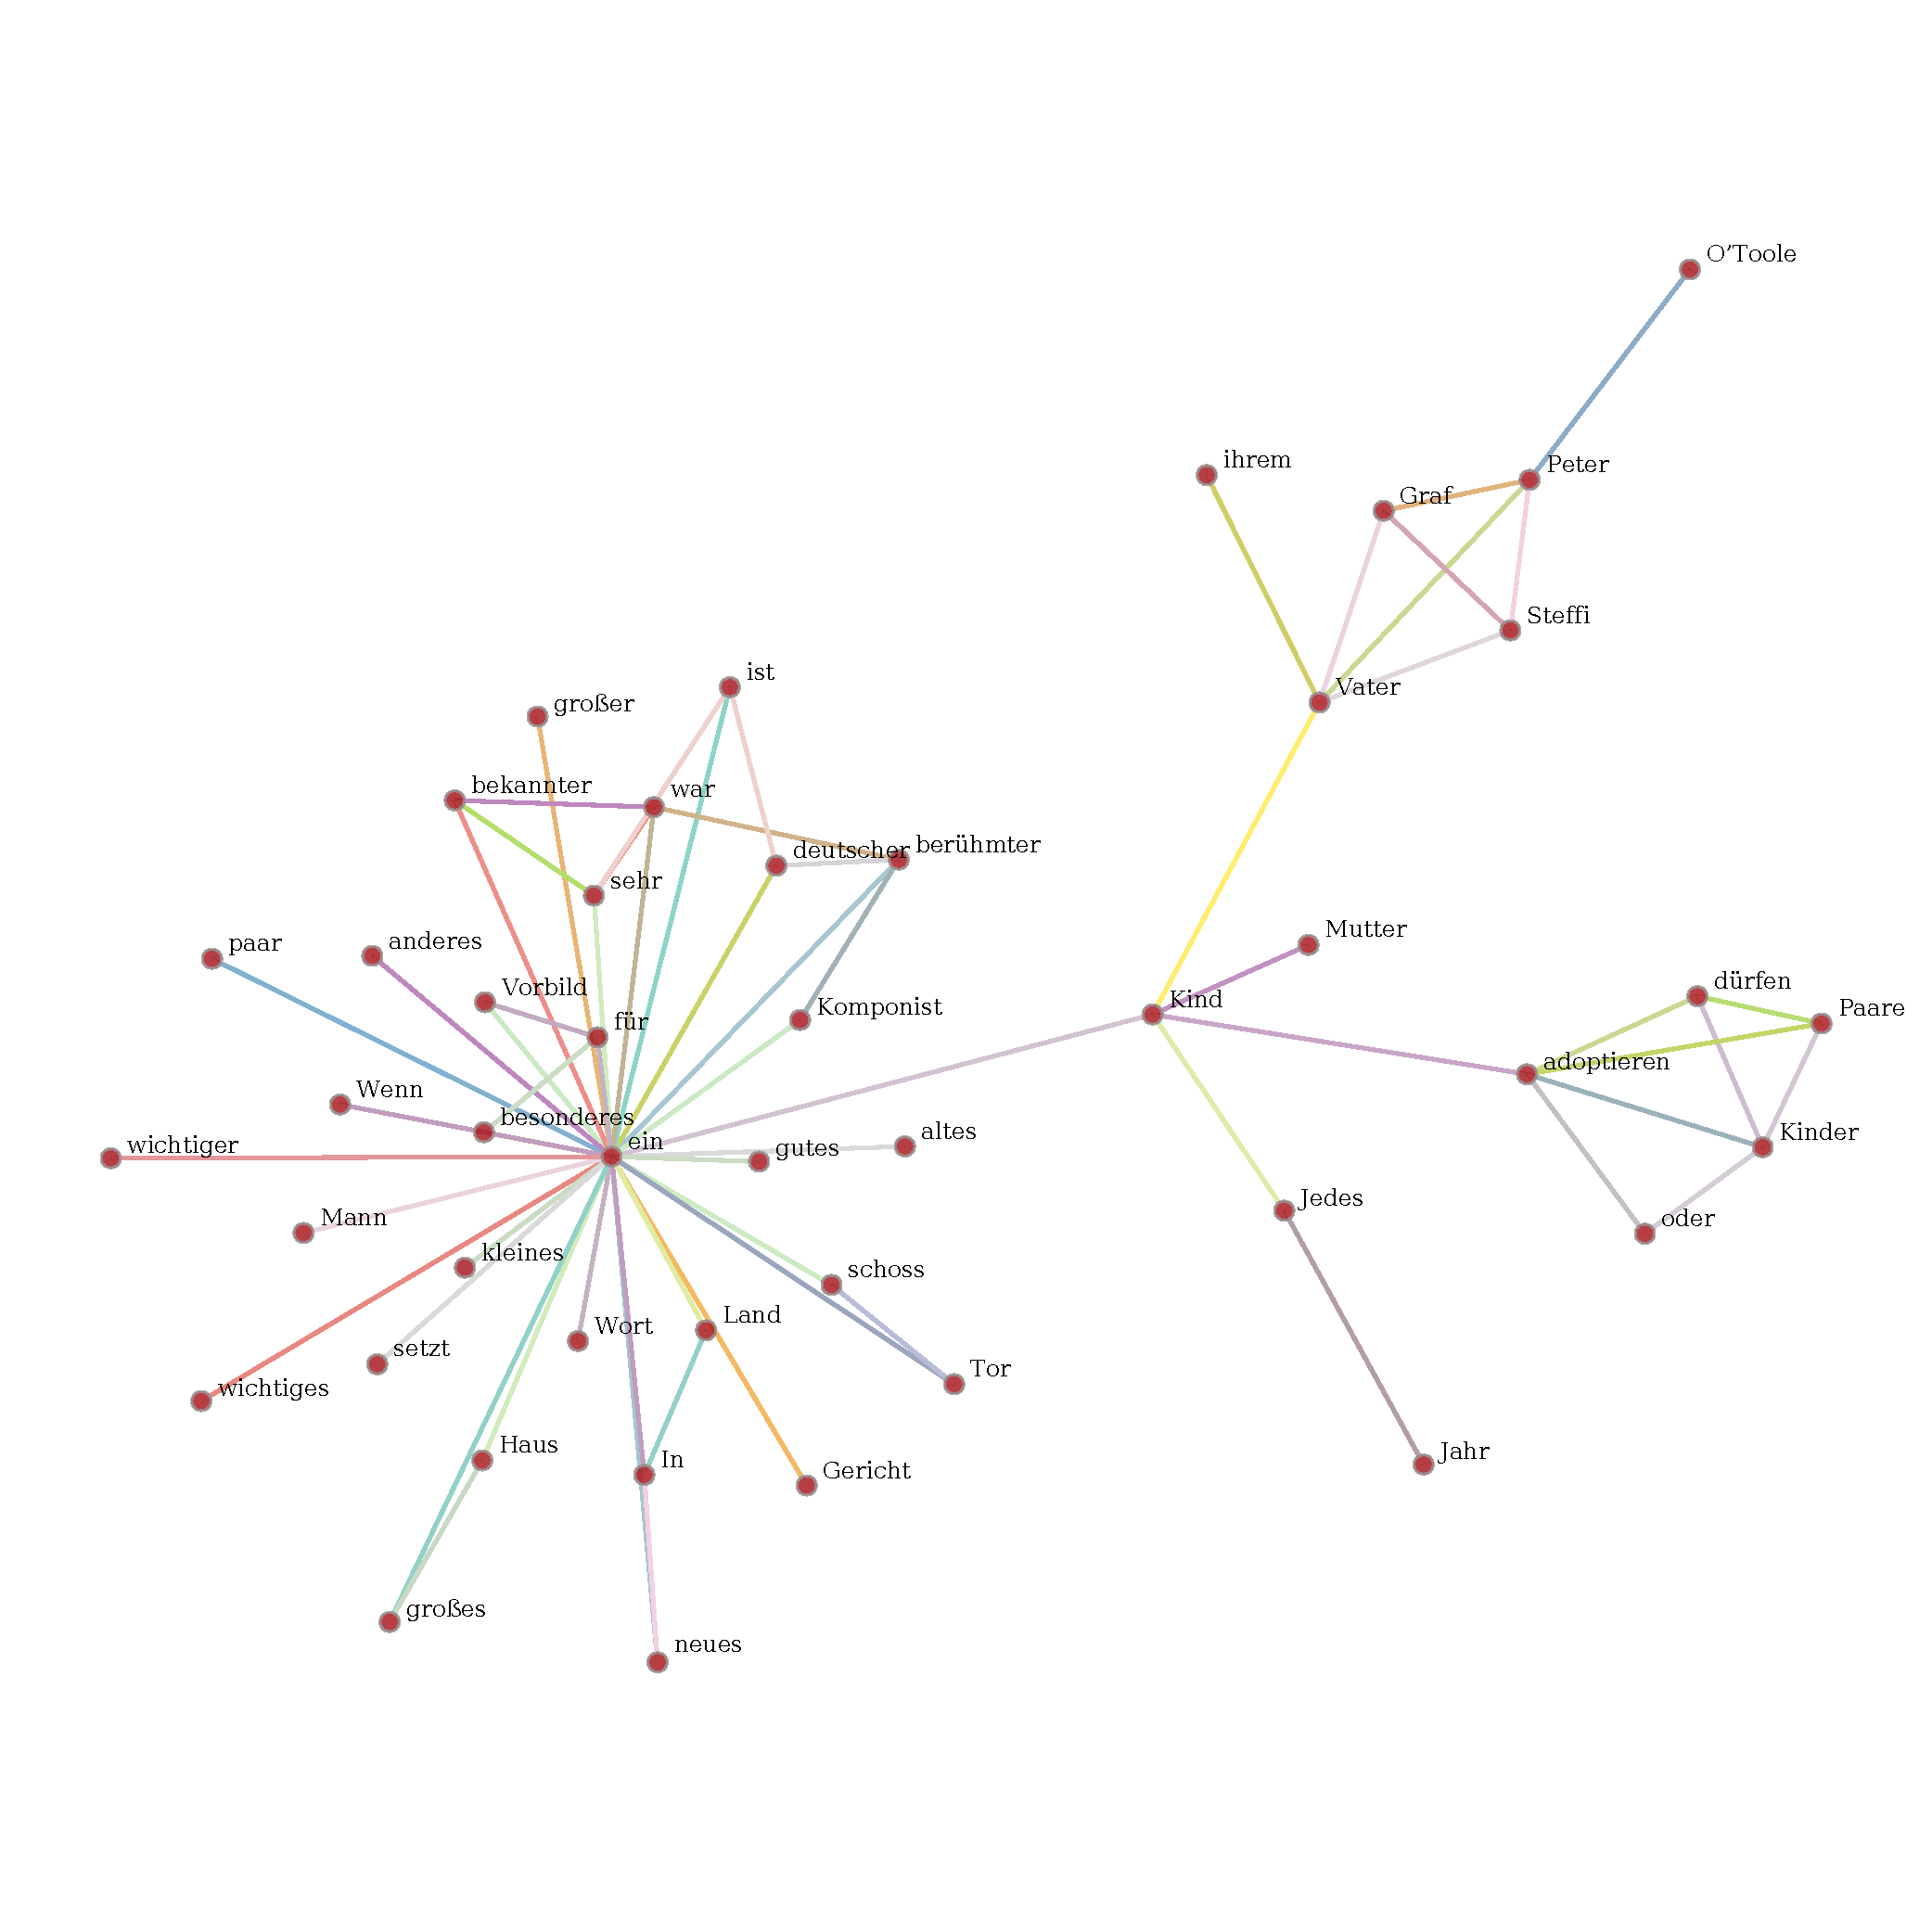
\includegraphics[scale=.4]{../../data/results/longpath_wordgraphs/nl/graph_OToole.pdf}
    \caption{Kookkurrenzgraph O’Toole (Distanz 5, Schwellwert 0,05)}
    \label{fig:lp-otoole}
\end{figure}

\begin{figure}[hp!]
    \centering
        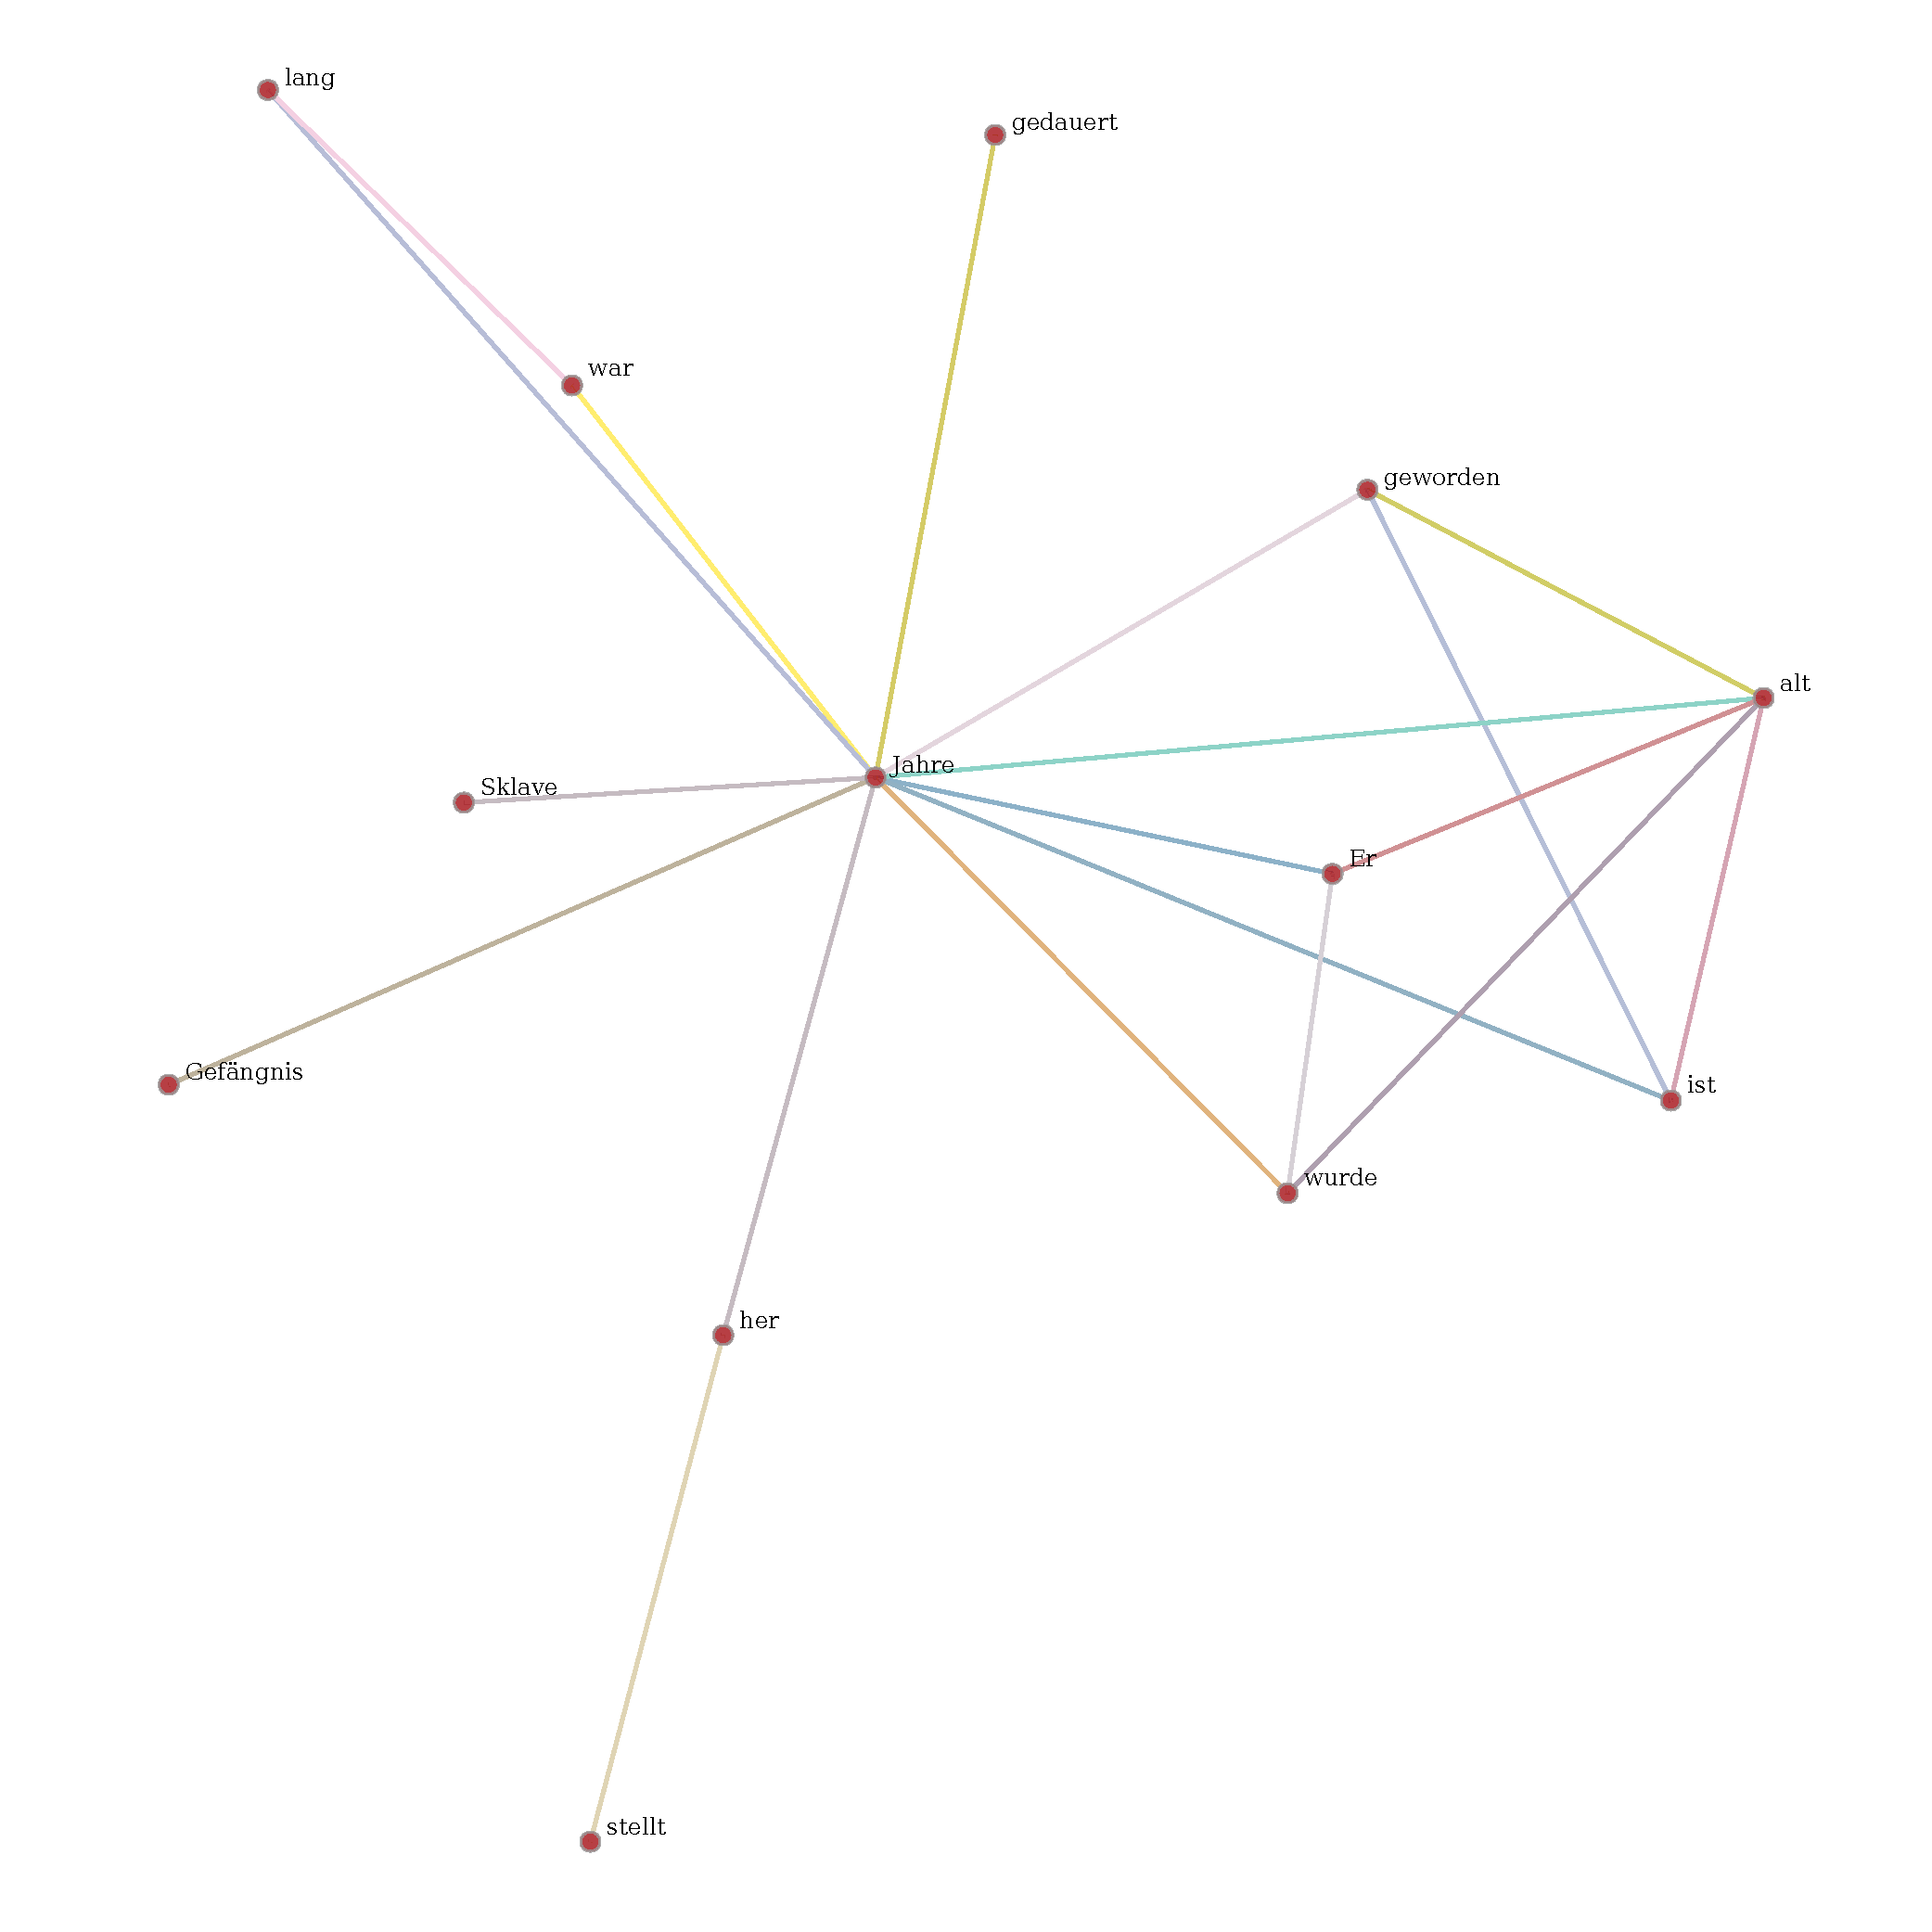
\includegraphics[scale=.4]{../../data/results/longpath_wordgraphs/nl/graph_stellt.pdf}
    \caption{Kookkurrenzgraph stellt (Distanz 3, Schwellwert 0,05)}
    \label{fig:lp-stellt}
\end{figure}


\pagebreak
\subsubsection{deunews2010\_10K}

\begin{figure}[hp!]
    \centering
        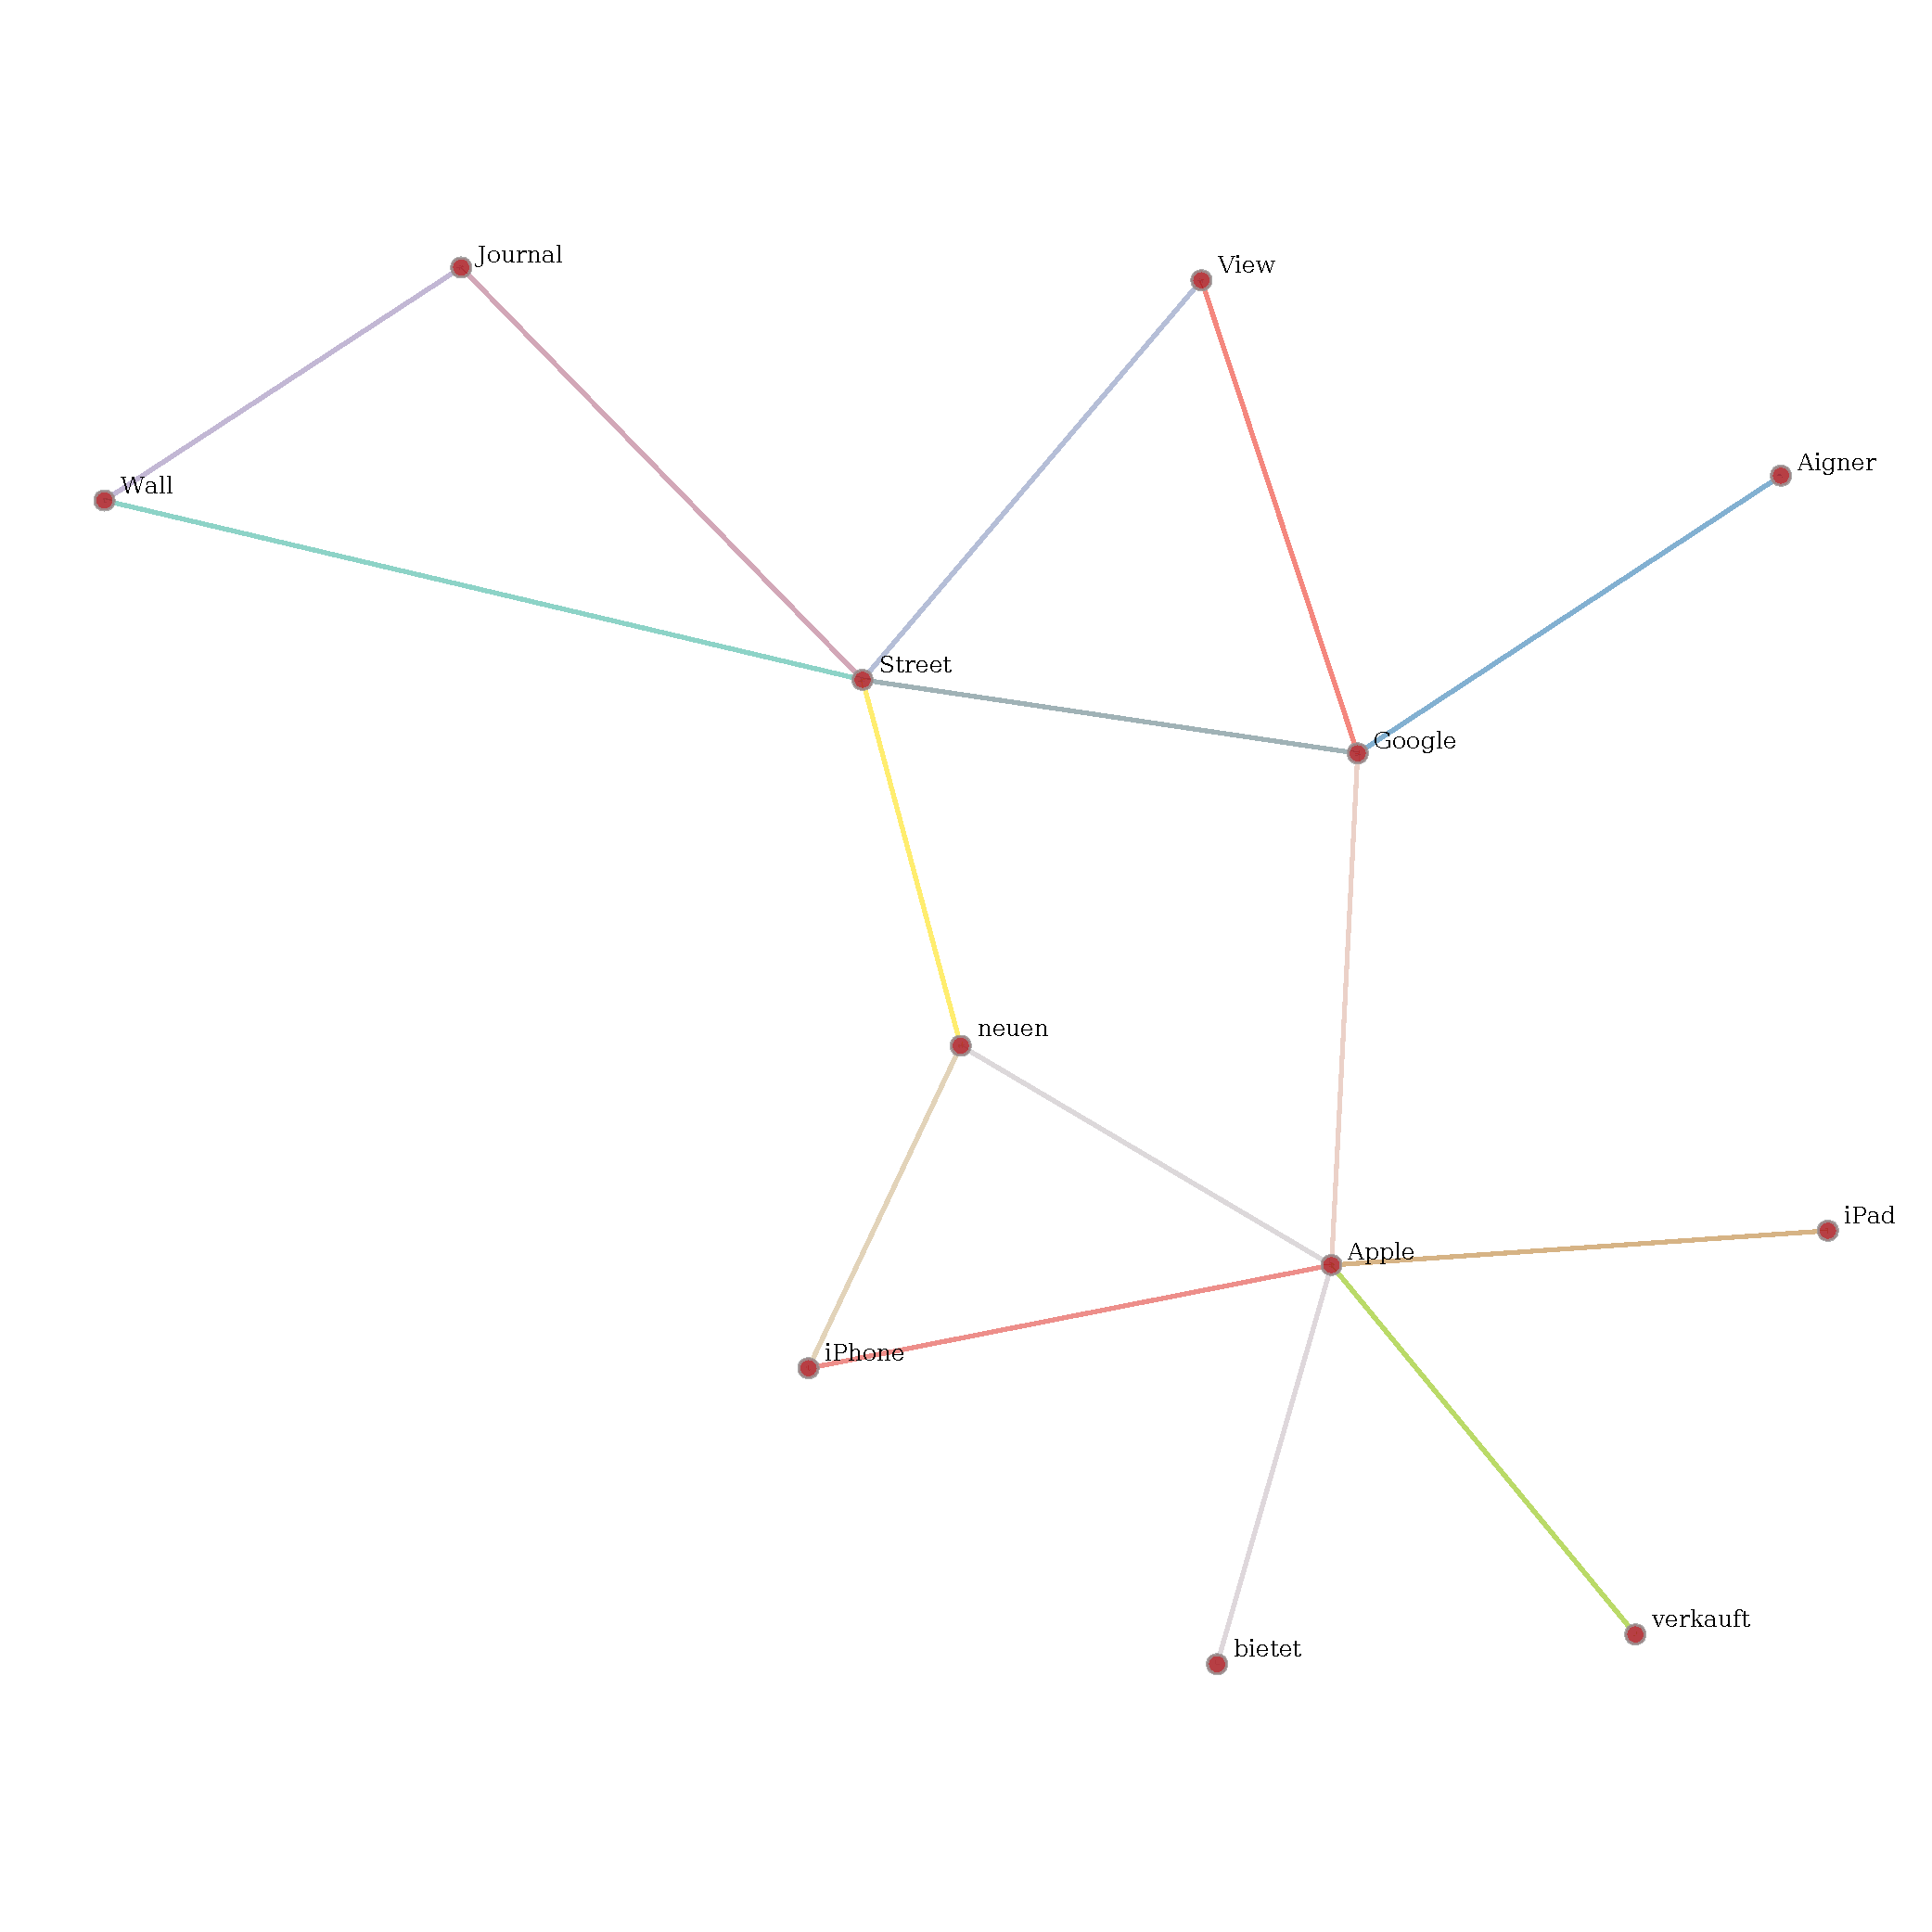
\includegraphics[scale=.4]{../../data/results/longpath_wordgraphs/den/graph_Aigner.pdf}
    \caption{Kookkurrenzgraph Aigner (Distanz 3, Schwellwert 0,1)}
    \label{fig:lp-aigner}
\end{figure}

\begin{figure}[hp!]
    \centering
        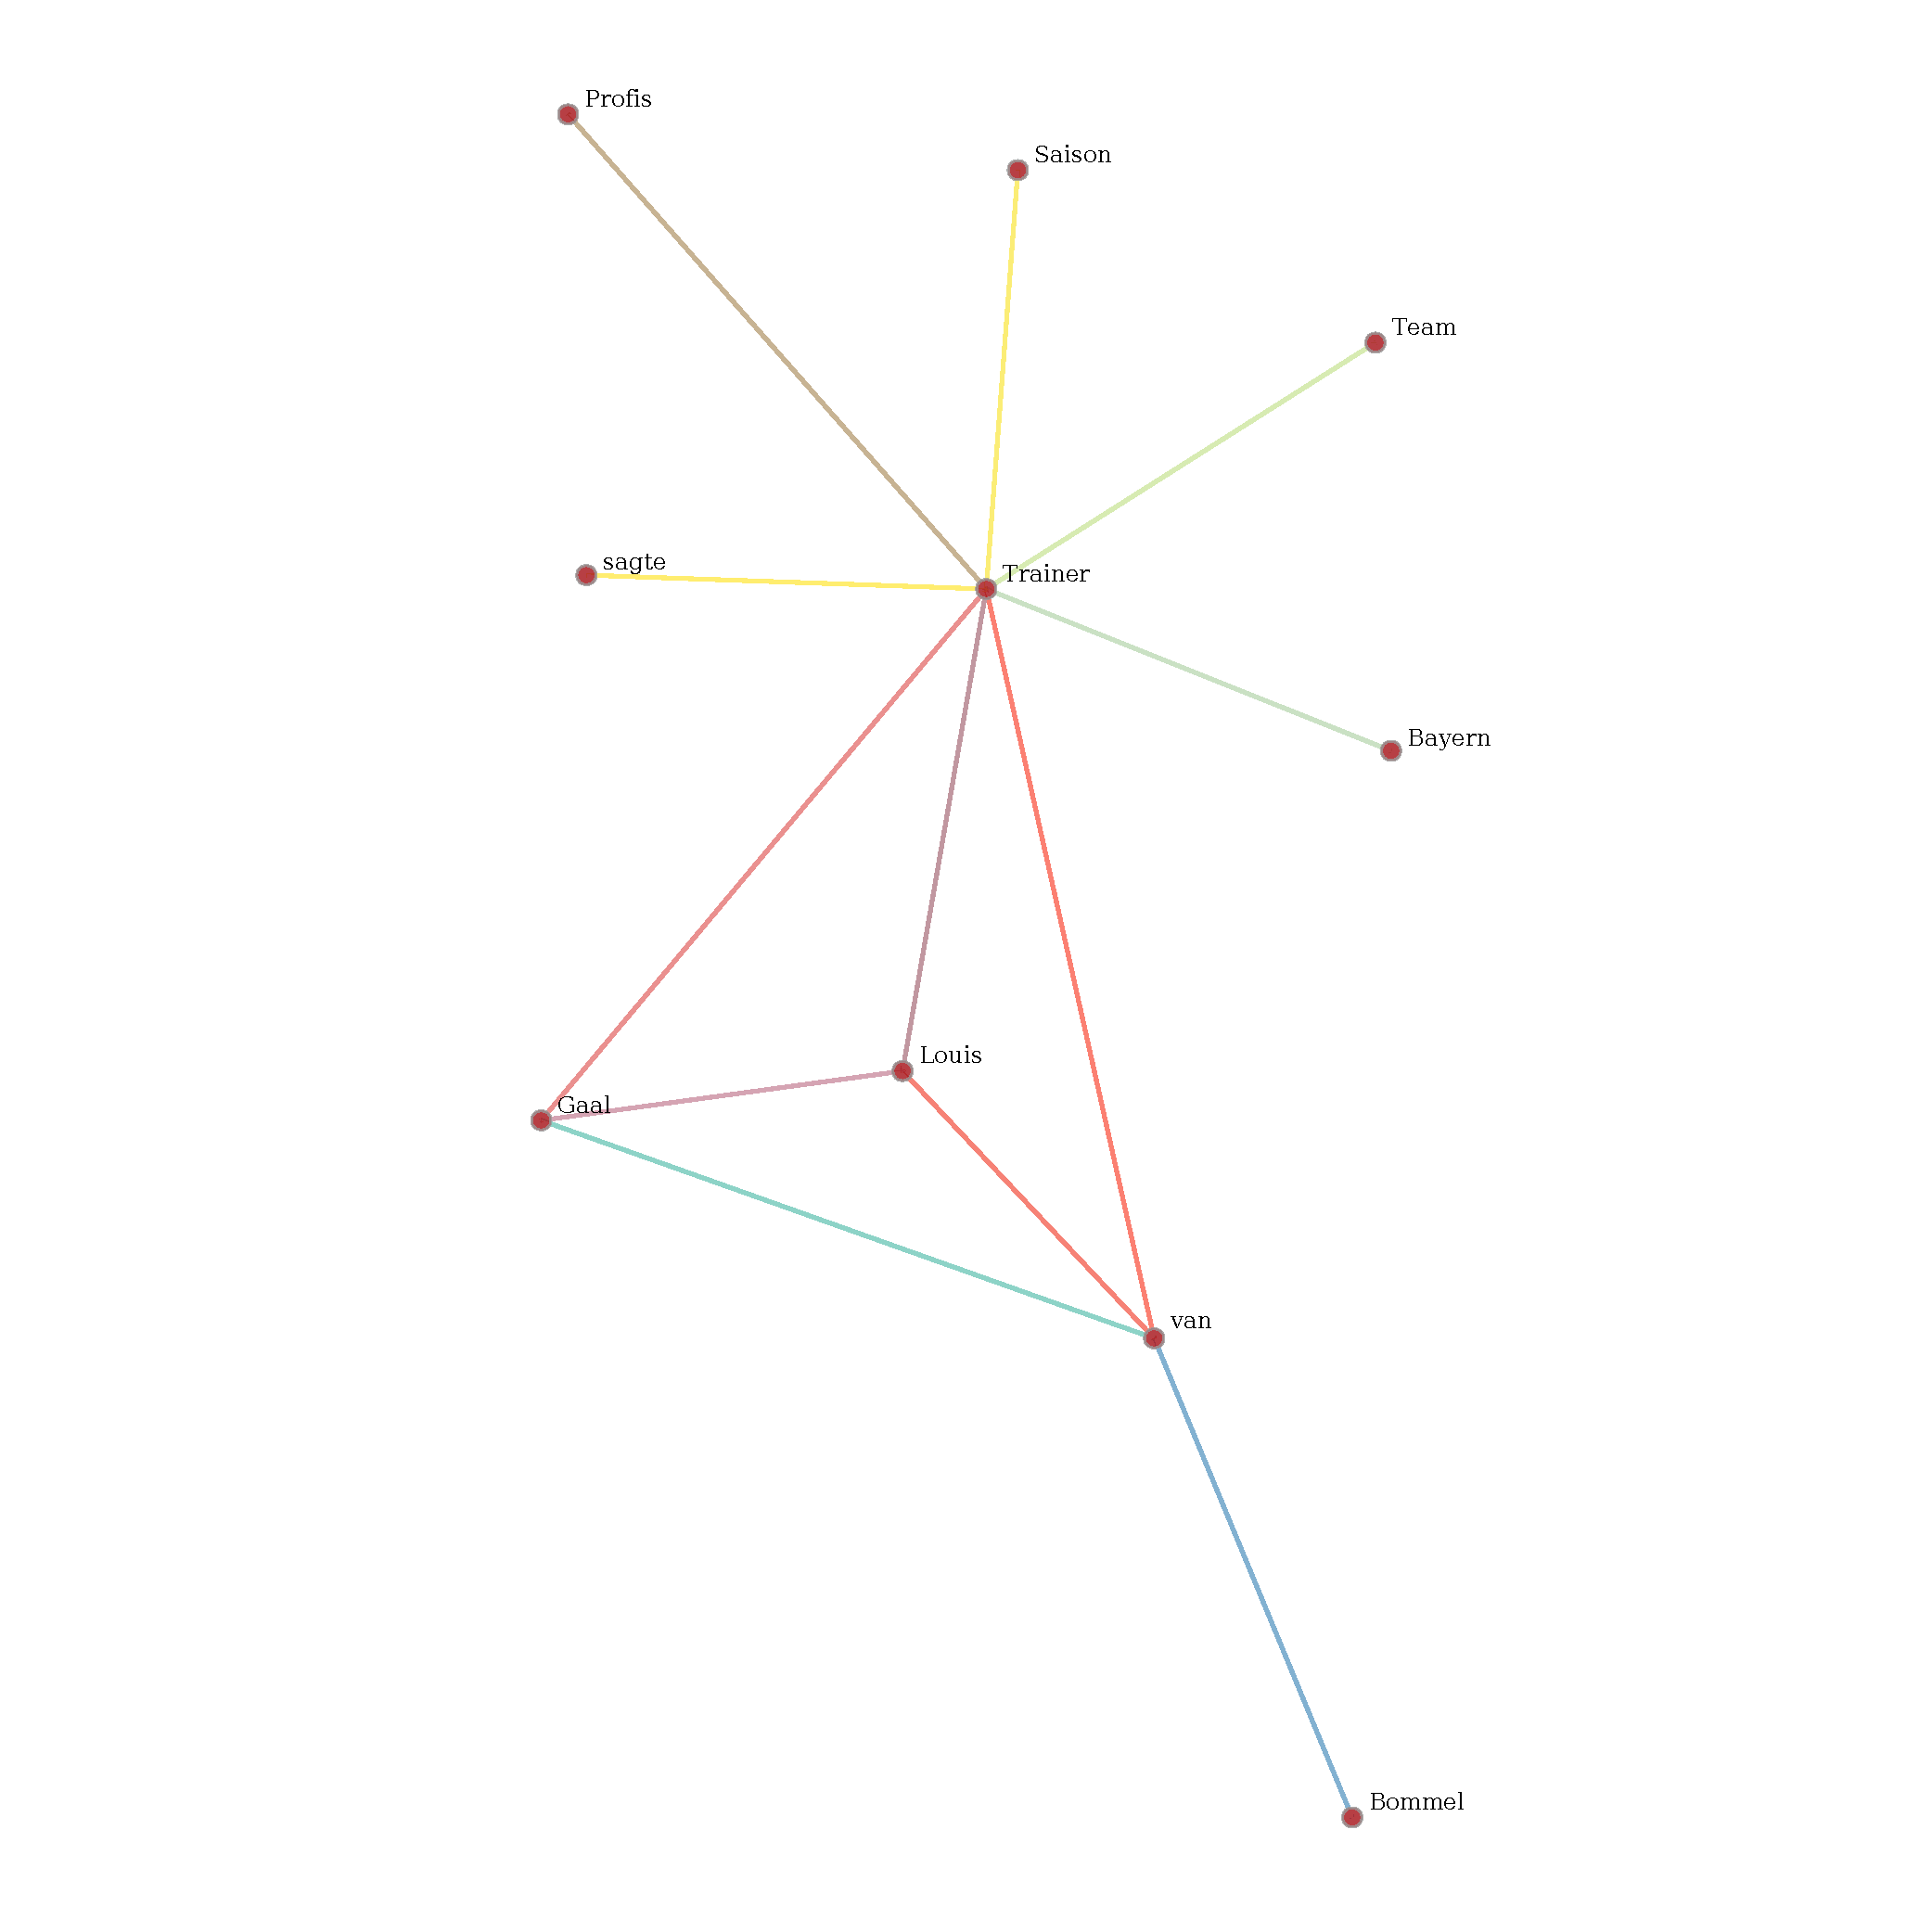
\includegraphics[scale=.4]{../../data/results/longpath_wordgraphs/den/graph_Bommel.pdf}
    \caption{Kookkurrenzgraph Bommel (Distanz 3, Schwellwert 0,1)}
    \label{fig:lp-bommel}
\end{figure}

\begin{figure}[hp!]
    \centering
        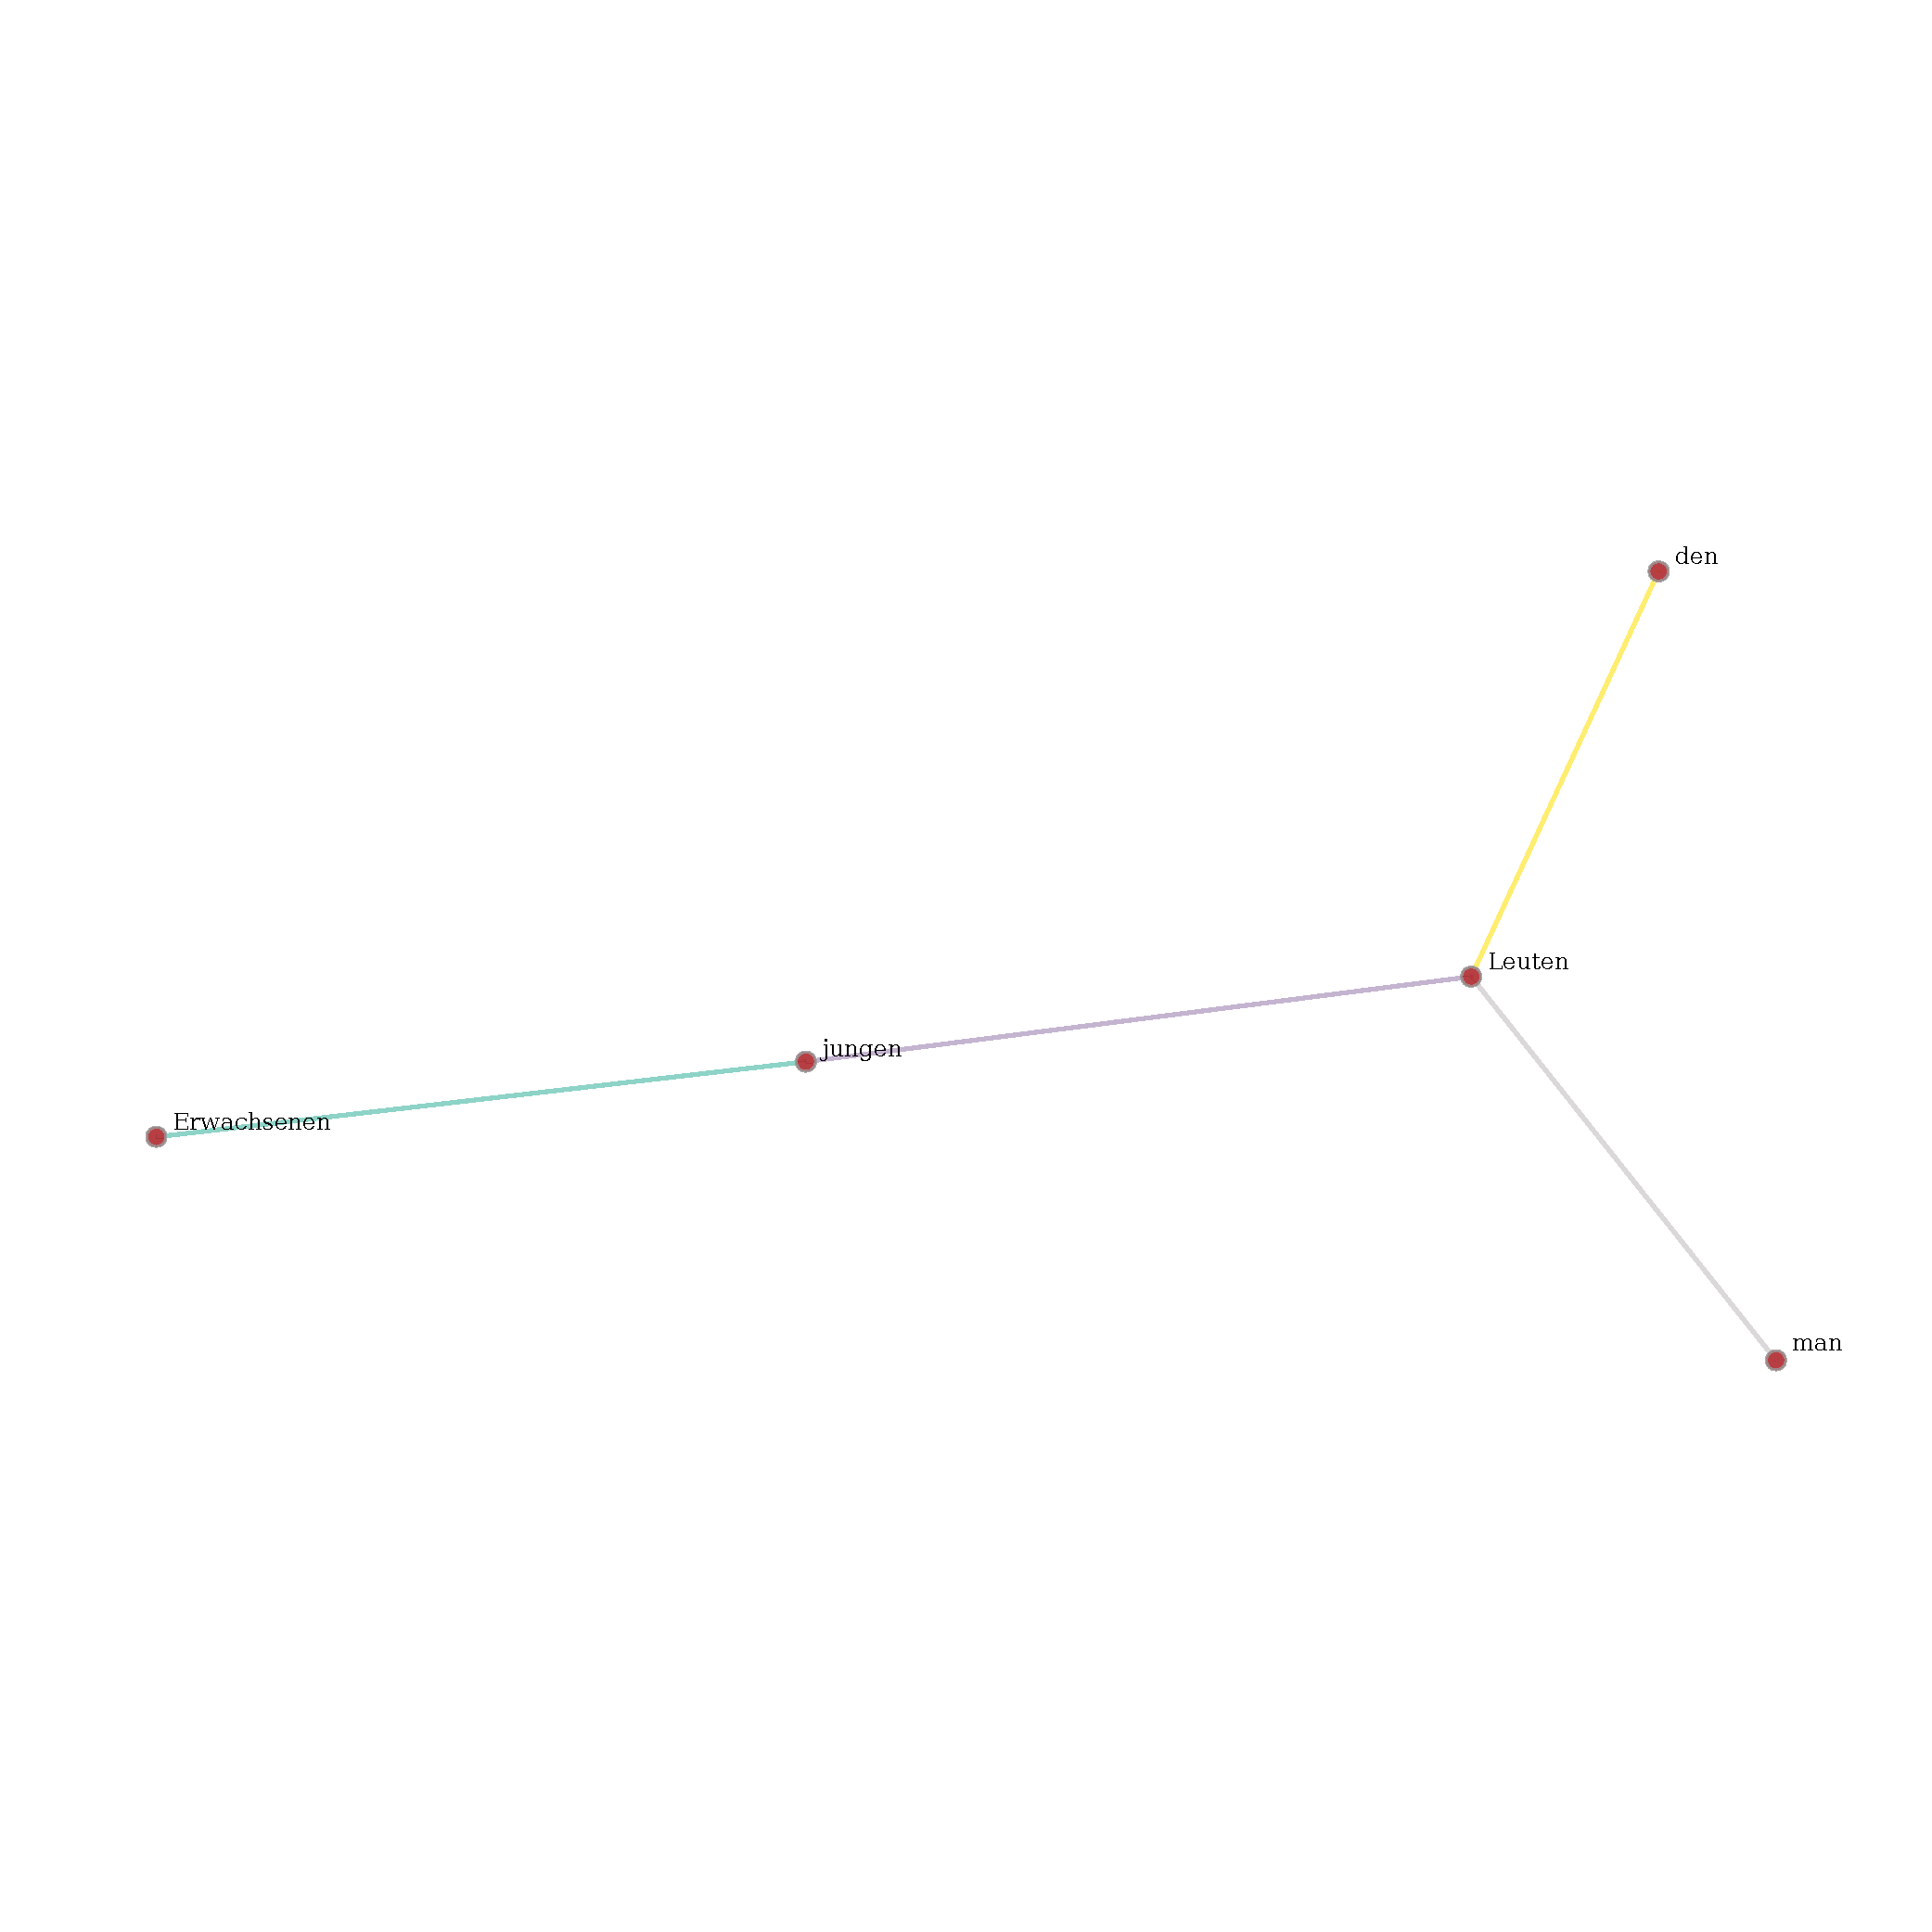
\includegraphics[scale=.4]{../../data/results/longpath_wordgraphs/den/graph_Erwachsenen.pdf}
    \caption{Kookkurrenzgraph Erwachsenen (Distanz 3, Schwellwert 0,5)}
    \label{fig:lp-erwachsenen}
\end{figure}

\begin{figure}[hp!]
    \centering
        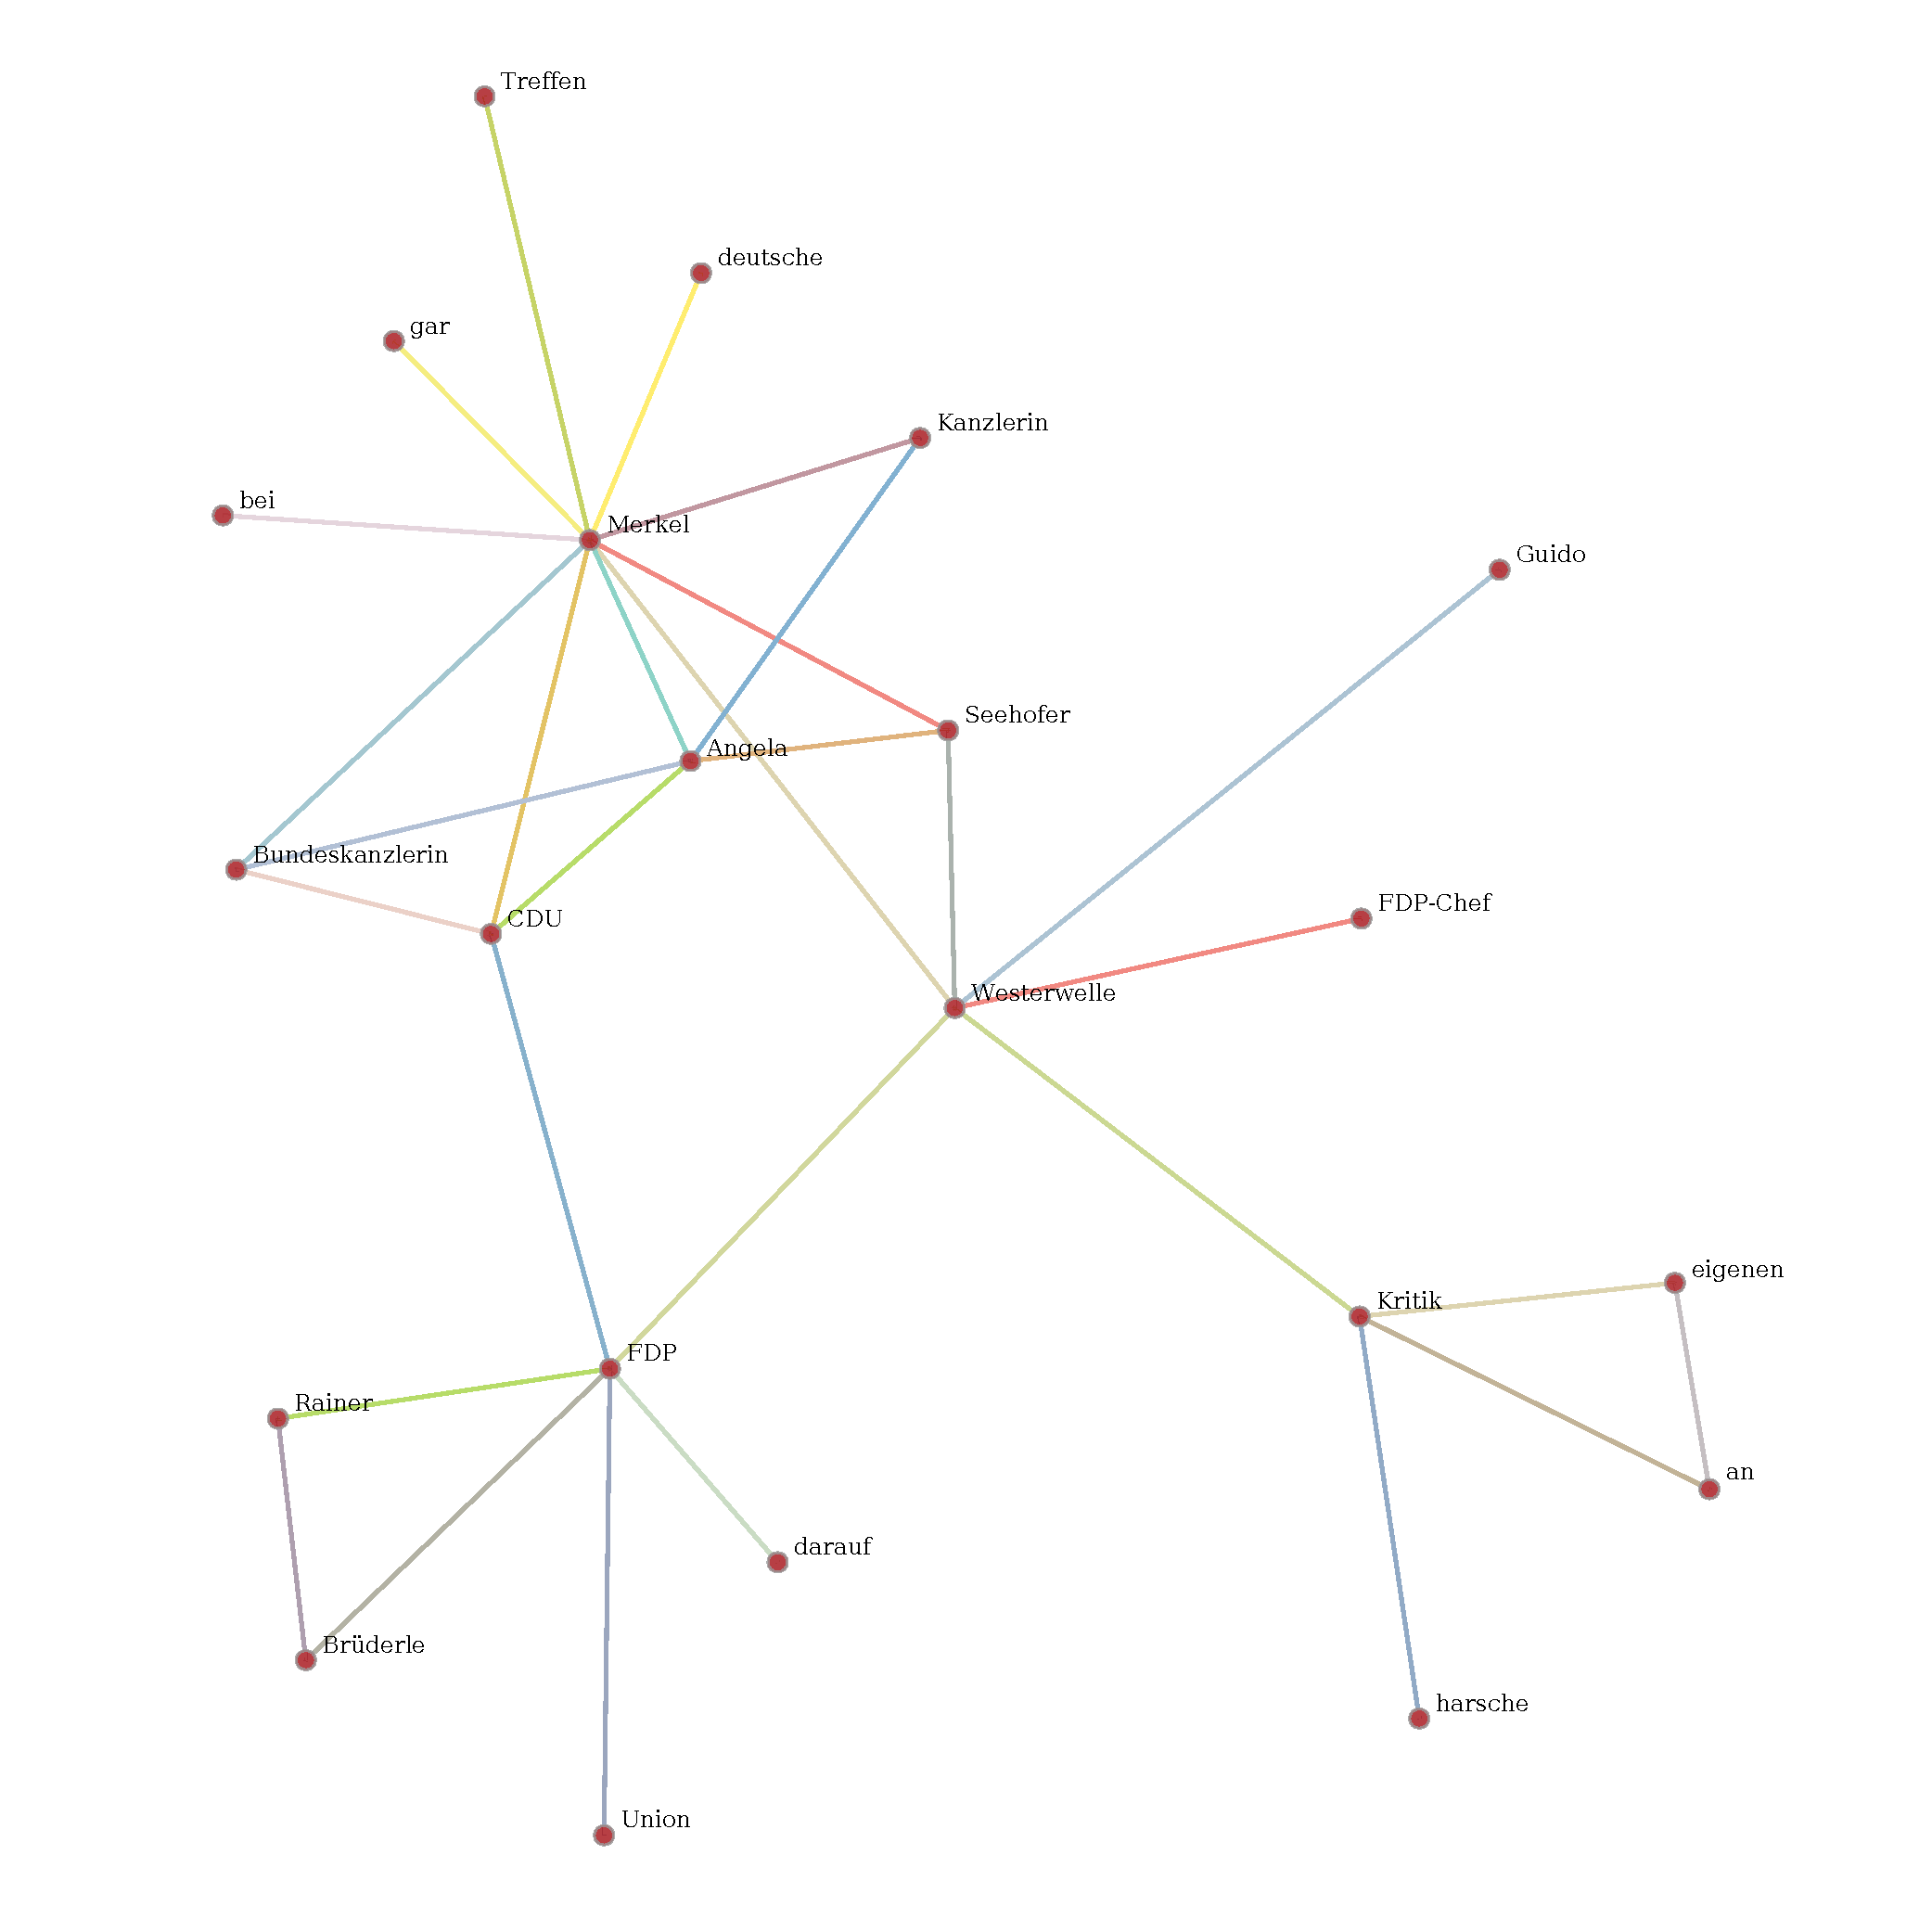
\includegraphics[scale=.4]{../../data/results/longpath_wordgraphs/den/graph_Guido.pdf}
    \caption{Kookkurrenzgraph Guido (Distanz 3, Schwellwert 0,1)}
    \label{fig:lp-guido}
\end{figure}

\begin{figure}[hp!]
    \centering
        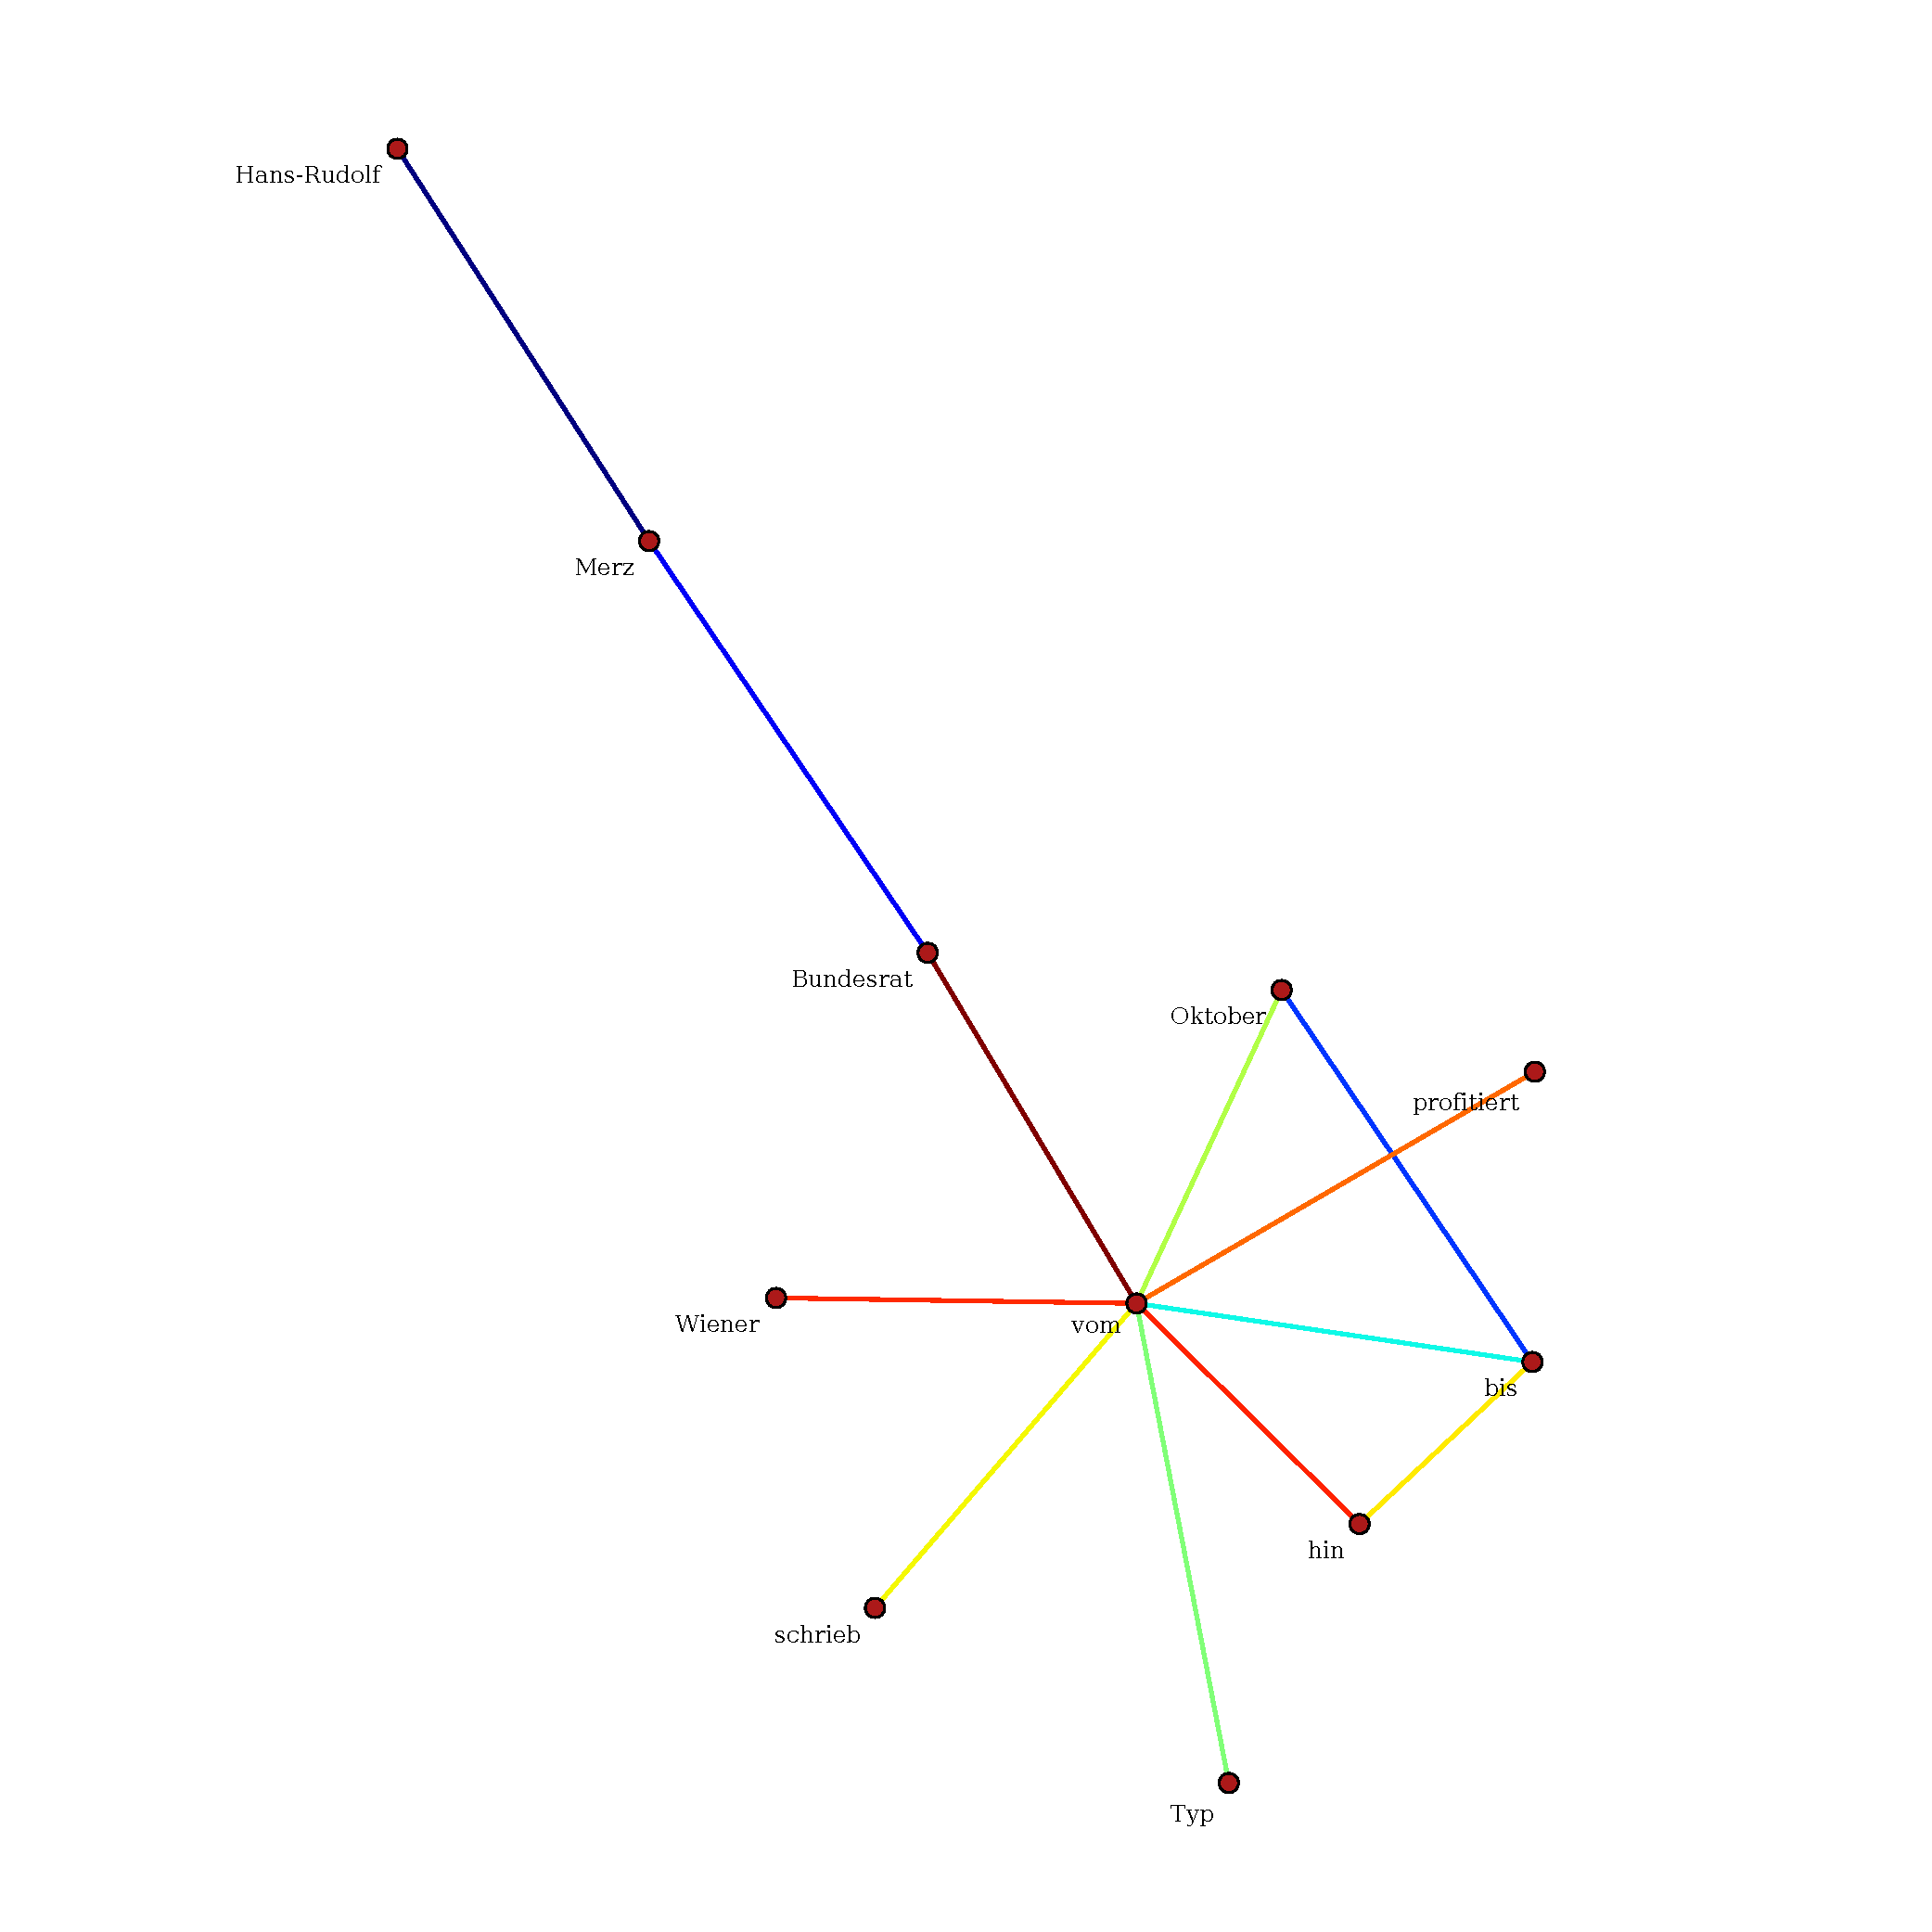
\includegraphics[scale=.4]{../../data/results/longpath_wordgraphs/den/graph_HansRudolf.pdf}
    \caption{Kookkurrenzgraph Hans-Rudolf (Distanz 4, Schwellwert 0,1)}
    \label{fig:lp-hansrudolf}
\end{figure}

\begin{figure}[hp!]
    \centering
        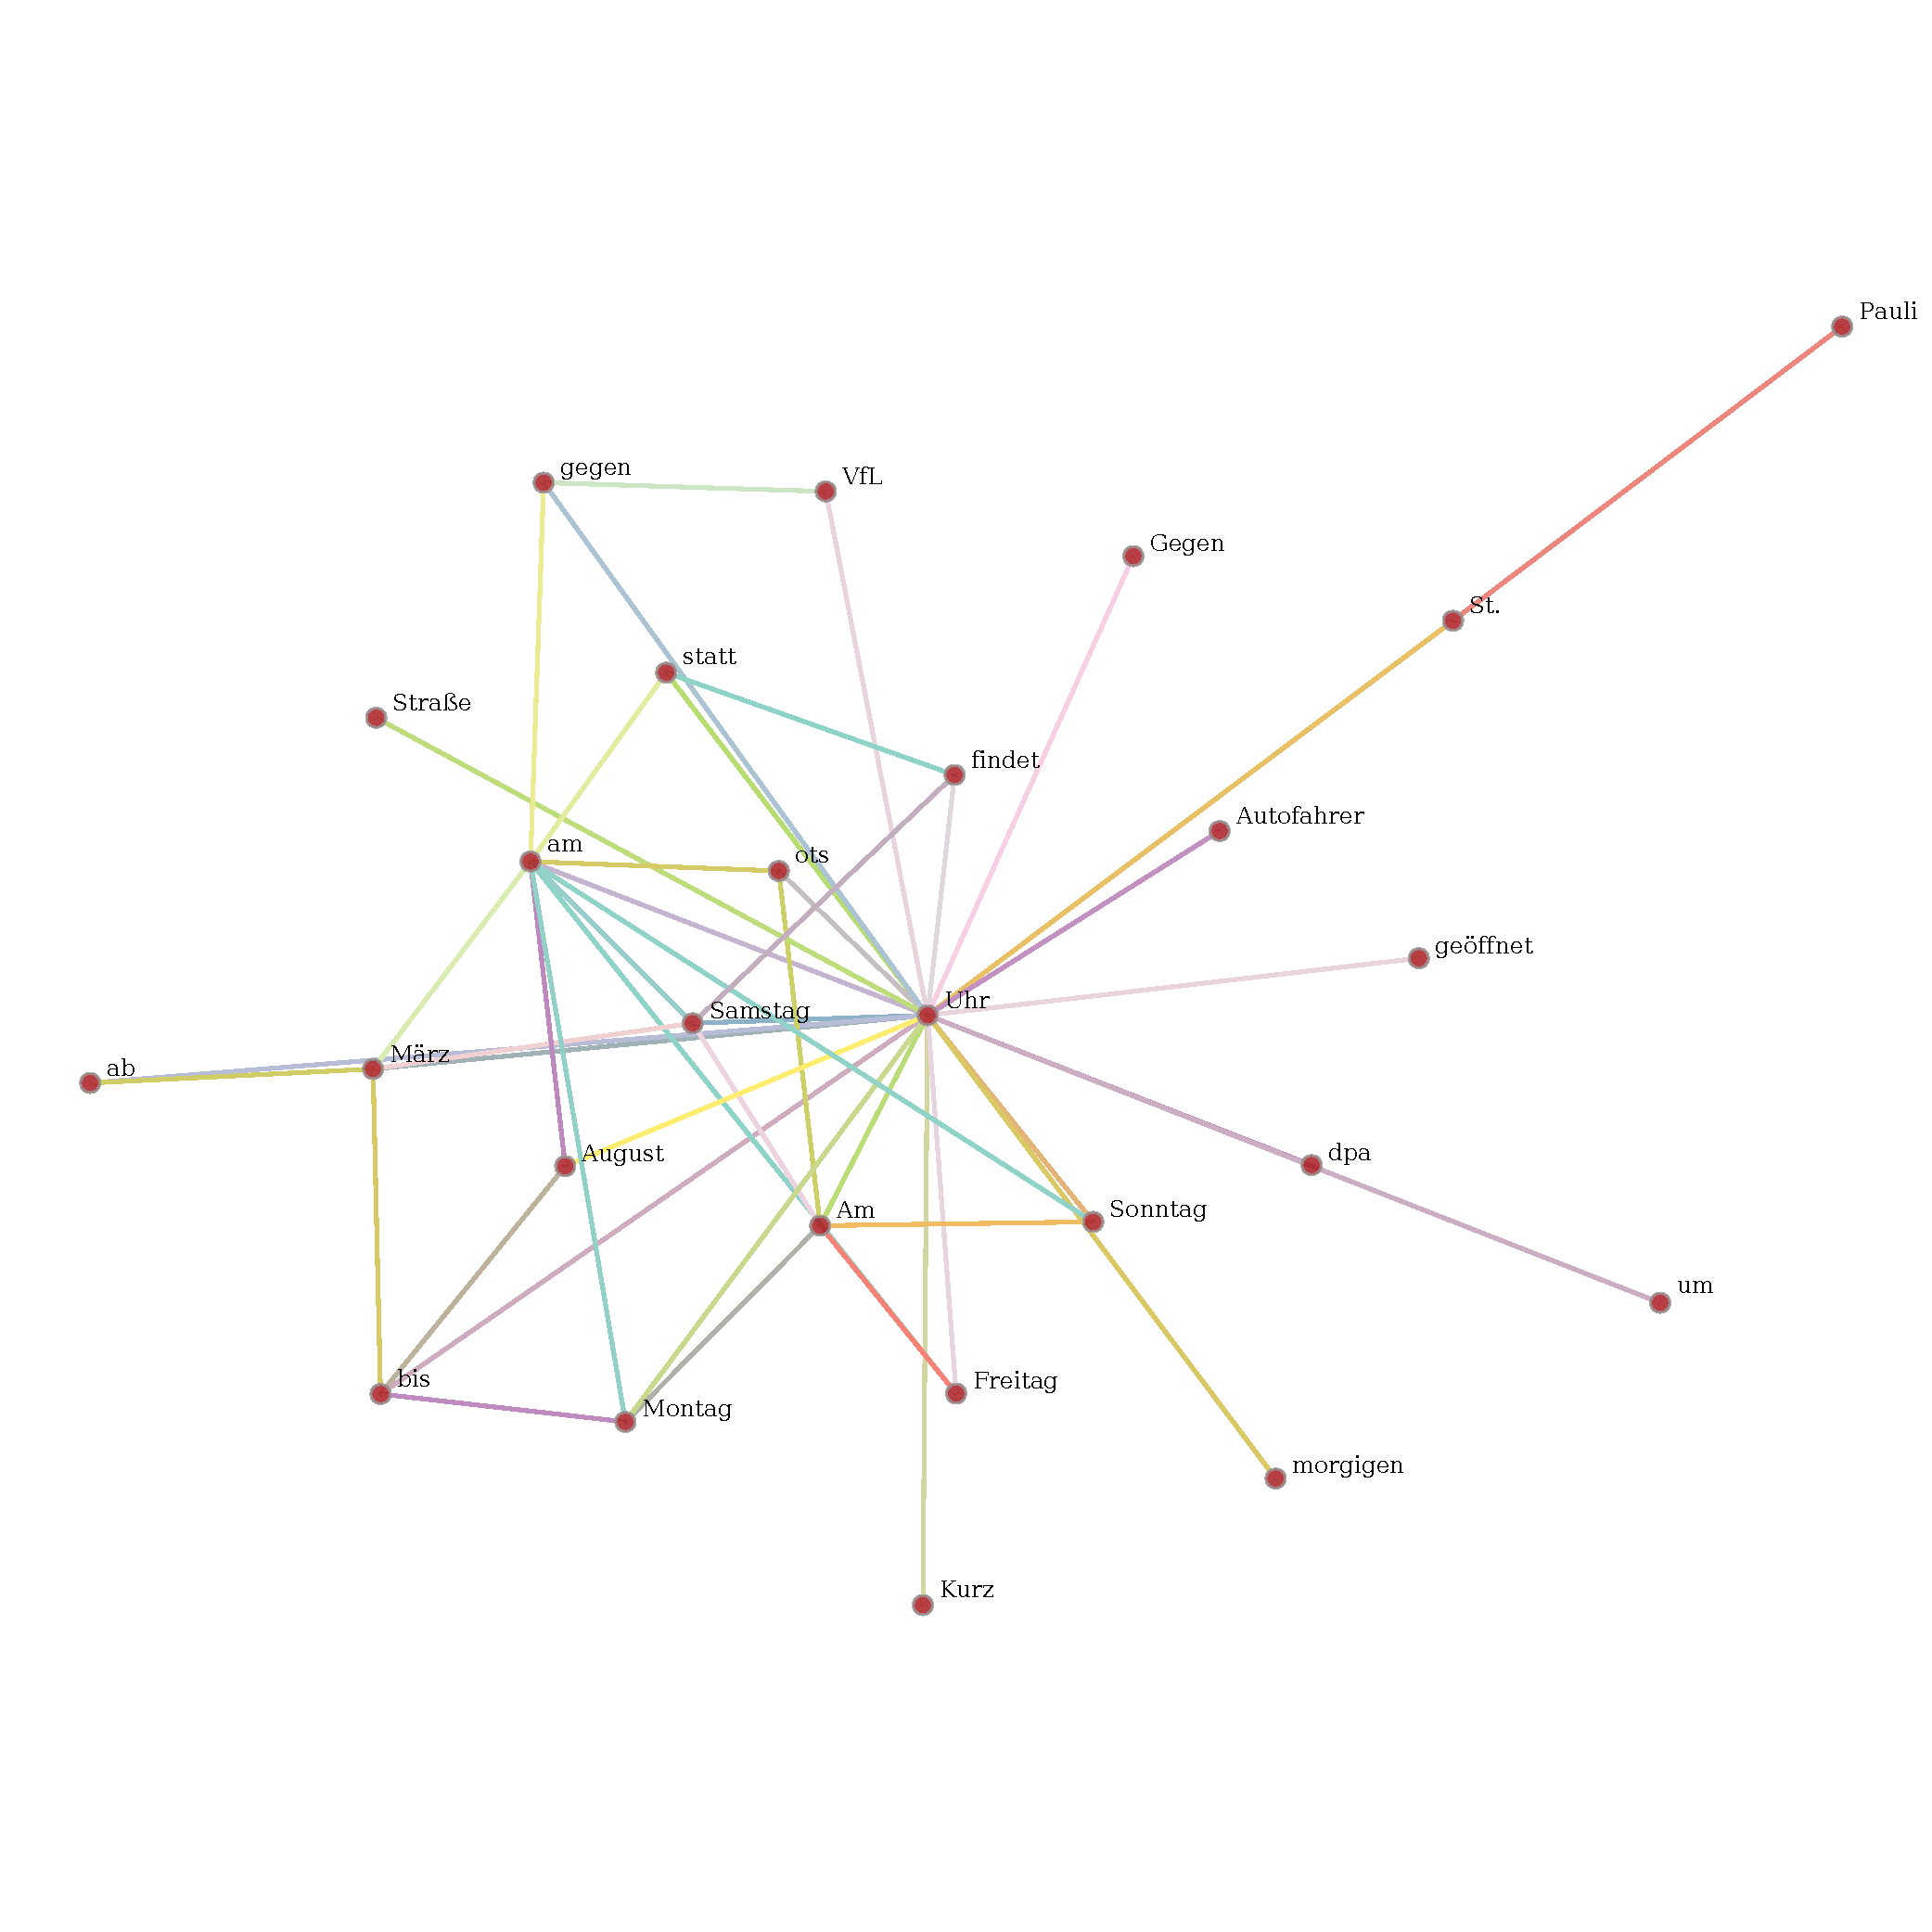
\includegraphics[scale=.4]{../../data/results/longpath_wordgraphs/den/graph_Pauli.pdf}
    \caption{Kookkurrenzgraph Pauli (Distanz 3, Schwellwert 0,1)}
    \label{fig:lp-pauli}
\end{figure}


%%%%%%%%%%%%%%%%%%%%%%%%%%%%%%%%%%%%%%%%%%%%%%%%%%%%%%%%%%%%%%%%%%%%%%%%%%%%%%%%
\pagebreak
\begin{thebibliography}{9}
% TODO:
% - remove unused citations/bibitems
% - sort remaining ones in order of appearance in the text
    \bibitem{Newman2003} M. E. J. Newman, “The Structure and Function of Complex Networks,” \emph{SIAM Review}, vol. 45, no. 2, pp. 167–256, 2003.
    \bibitem{Biemann2004} C. Biemann, S. Bordag, G. Heyer, U. Quasthoff, and C. Wolff, “Language-Independent Methods for Compiling Monolingual Lexical Data,” in \emph{Computational Linguistics and Intelligent Text Processing}, vol. 2945, A. Gelbukh, Ed. Berlin, Heidelberg: Springer Berlin Heidelberg, 2004, pp. 217–228.
    \bibitem{Hu2006} Y. Hu, “Efficient, High-Quality Force-Directed Graph Drawing,” \emph{The Mathematica Journal}, vol. 10, no. 1, pp. 37–71, 2006.
    \bibitem{Quasthoff2006}U. Quasthoff, M. Richter, and C. Biemann, “Corpus Portal for Search in Monolingual Corpora,” in \emph{Proceedings of LREC-06}, Genoa, Italy, 2006, pp. 1799–1802.
    \bibitem{Telesford2011}Q. K. Telesford, K. E. Joyce, S. Hayasaka, J. H. Burdette, and P. J. Laurienti, “The Ubiquity of Small-World Networks,” \emph{Brain Connectivity}, vol. 1, no. 5, pp. 367–375, 2011.
    \bibitem{nls_regeln} Das Netzwerk Leichte Sprache, “Die Regeln für Leichte Sprache”, 2013. \url{http://leichtesprache.org/images/Regeln_Leichte_Sprache.pdf} (zuletzt geprüft: 17. April 2015).
    \bibitem{Humphries2006}M. Humphries, K. Gurney, and T. Prescott, “The brainstem reticular formation is a small-world, not scale-free, network,” in \emph{Proceedings of the Royal Society B: Biological Sciences}, vol. 273(1585), pp. 503–511, 2006.
\end{thebibliography}

\listoftables

\listoffigures

\end{document}
